%%%%%%%%%%%%%%%%%%%%%%%%%%%%%%%%%%%%%%%%%%%%%%%%%%%% 
%%%     Language Science Press Master File       %%%
%%%         follow the instructions below        %%% 
%%%%%%%%%%%%%%%%%%%%%%%%%%%%%%%%%%%%%%%%%%%%%%%%%%%%
 
% Everything following a % is ignored
% Some lines start with %. Remove the % to include them

\documentclass[output=book,nonflat,modfonts,
  colorlinks,citecolor=brown, 
%  draft,draftmode,  
%  showindex,
%  nobabel,
 booklanguage=english,
%  multiauthors,
		  ]{langsci/langscibook}    
  
%%%%%%%%%%%%%%%%%%%%%%%%%%%%%%%%%%%%%%%%%%%%%%%%%%%% 
%%%          additional packages                 %%% 
%%%%%%%%%%%%%%%%%%%%%%%%%%%%%%%%%%%%%%%%%%%%%%%%%%%% 

\title{Representational considerations in models of language change and stability}
\author{Rebecca L. Morley}
\subtitle{}

\BackBody{Research in linguistics, as in most other scientific domains, is usually approached in a modular way – narrowing the domain of inquiry in order to allow for increased depth of study. This is necessary and productive for a topic as wide-ranging and complex as human language. However, precisely because language is a complex system, tied to perception, learning, memory, and social organization, the assumption of modularity can also be an obstacle to understanding language at a deeper level. 

The methodological focus of this work is on computational modeling, highlighting two aspects of modeling work that receive relatively little attention: the formal mapping from model to theory, and the scalability of demonstration models. A series of implemented models of sound change are analyzed in this way. As theoretical inconsistencies are discovered, possible solutions are proposed, incrementally constructing a set of sufficient properties for a working model. Because internal theoretical consistency is enforced, this model corresponds to an explanatorily adequate theory. And because explicit links between modules are required, this is a theory, not only of sound change, but of many aspects of phonological competence.}
%\dedication{Change dedication in localmetadata.tex}
\typesetter{Felix Kopecky, Rebecca L. Morley}
% \proofreader{}

\BookDOI{10.5281/zenodo.3264909}%ask coordinator for DOI
\renewcommand{\lsISBNdigital}{978-3-96110-190-0}
\renewcommand{\lsISBNhardcover}{978-3-96110-191-7}
\renewcommand{\lsSeries}{cfls} % use lowercase acronym, e.g. cfls, sidl, eotms, tgdi
\renewcommand{\lsSeriesNumber}{4} %will be assigned when the book enters the proofreading stage
\renewcommand{\lsID}{251} % contact the coordinator for the right number

% add all extra packages you need to load to this file  
\usepackage{tabularx} 
\usepackage{url} 
\urlstyle{same}

\usepackage{listings}
\lstset{basicstyle=\ttfamily,tabsize=2,breaklines=true}


%%%%%%%%%%%%%%%%%%%%%%%%%%%%%%%%%%%%%%%%%%%%%%%%%%%%
%%%                                              %%%
%%%           Examples                           %%%
%%%                                              %%%
%%%%%%%%%%%%%%%%%%%%%%%%%%%%%%%%%%%%%%%%%%%%%%%%%%%% 
%% to add additional information to the right of examples, uncomment the following line
% \usepackage{jambox}
%% if you want the source line of examples to be in italics, uncomment the following line
% \renewcommand{\exfont}{\itshape}
\usepackage{langsci-optional}
\usepackage{./langsci/styles/langsci-lgr}
 
\usepackage{multirow}
\usepackage{colortbl}
\usepackage{enumitem}

\@ifundefined{showcaptionsetup}{}{%
	\PassOptionsToPackage{caption=false}{subfig}}
\usepackage{subfig}
\makeatother

\usepackage{xunicode}
\usepackage{covington}
\usepackage{polyglossia}

\usepackage{langsci-gb4e}
%% hyphenation points for line breaks
%% Normally, automatic hyphenation in LaTeX is very good
%% If a word is mis-hyphenated, add it to this file
%%
%% add information to TeX file before \begin{document} with:
%% %% hyphenation points for line breaks
%% Normally, automatic hyphenation in LaTeX is very good
%% If a word is mis-hyphenated, add it to this file
%%
%% add information to TeX file before \begin{document} with:
%% %% hyphenation points for line breaks
%% Normally, automatic hyphenation in LaTeX is very good
%% If a word is mis-hyphenated, add it to this file
%%
%% add information to TeX file before \begin{document} with:
%% \include{localhyphenation}
\hyphenation{
Dub-lin
wheth-er
}

\hyphenation{
Dub-lin
wheth-er
}

\hyphenation{
Dub-lin
wheth-er
}

\addbibresource{localbibliography.bib}

%%%%%%%%%%%%%%%%%%%%%%%%%%%%%%%%%%%%%%%%%%%%%%%%%%%% 
%%%             Frontmatter                      %%% 
%%%%%%%%%%%%%%%%%%%%%%%%%%%%%%%%%%%%%%%%%%%%%%%%%%%% 
\begin{document} 
\newcommand{\appref}[1]{Appendix \ref{#1}}
\newcommand{\fnref}[1]{Footnote \ref{#1}} 

\newenvironment{langscibars}{\begin{axis}[ybar,xtick=data, xticklabels from table={\mydata}{pos}, 
        width  = \textwidth,
	height = .3\textheight,
    	nodes near coords, 
	xtick=data,
	x tick label style={},  
	ymin=0,
	cycle list name=langscicolors
        ]}{\end{axis}}
        
\newcommand{\langscibar}[1]{\addplot+ table [x=i, y=#1] {\mydata};\addlegendentry{#1};}

\newcommand{\langscidata}[1]{\pgfplotstableread{#1}\mydata;}

\XeTeXdashbreakstate=0 % don't allow line breaks after em/en dashes
\newcommand{\noun}[1]{\textsc{#1}}
%% Because html converters don't know tabularnewline
\providecommand{\tabularnewline}{\\}
%% A simple dot to overcome graphicx limitations
\newcommand{\lyxdot}{.}

% \bibpunct{(}{)}{,}{a}{,}{,}

\setenumerate[0]{label=(\alph*)}

\renewcommand{\multirowsetup}{\centering}
 
  
\maketitle                
\frontmatter 

\currentpdfbookmark{Contents}{name} % adds a PDF bookmark
{\sloppy\tableofcontents}
% \include{chapters/preface}
% \include{chapters/acknowledgments}
% \include{chapters/abbreviations} 
\mainmatter     
 
%%%%%%%%%%%%%%%%%%%%%%%%%%%%%%%%%%%%%%%%%%%%%%%%%%%% 
%%%             Chapters                         %%% 
%%%%%%%%%%%%%%%%%%%%%%%%%%%%%%%%%%%%%%%%%%%%%%%%%%%%

\chapter{Introduction}

Synchronic and diachronic linguistics are typically pursued as separate
disciplines, with little to no overlap. Nevertheless, it is not possible
for either to be truly agnostic about the form of the other. This
is necessarily true because synchronic theories are not theories about
attested languages, but theories about possible languages. Therefore,
any possible language, undergoing any series of diachronic changes,
must always end up as another member of the set of possible synchronic
languages. Conversely, a theory of the end state of diachronic change
is necessarily a theory of a synchronic grammar at some point in time.
The actuators of change must also be latently present in some way
within synchronic states, just as the speakers of daughter languages
must have been learners of mother languages.

In this work I will demonstrate how deeply held assumptions about
the correct representations of synchronic grammars delimit an associated
theory of diachrony, and how standard assumptions about the units
of change disallow certain synchronic states. I will argue that it
is necessary to reconsider the operative units within both domains,
and that in doing so we are likely to gain new insights into how linguistic
structures change and, by extension, how they fail to change, i.e.,
exhibit stable variation.

The goal of this work is to determine what types of mental structures
may be sufficient, and possibly, necessary in order to capture certain
linguistic phenomena at a computational level of description (in the
sense of \citet{marr1982vision}). The approach is twofold: 1) to
test a number of proposed structures and mechanisms by implementing
them in simple computational models; and 2) to test the explanatory
adequacy of a number of existing models by transforming their implementations
into theoretical constructs. The first method is likely to be familiar
to many readers; the second, however, is somewhat novel, and requires
some explanation. In the simplest terms, it is the reverse of the
first: taking implemented functions and deriving the theoretical linguistic
entity that the function implements. This requires determining whether
a specific implementational detail is incidental (with no repercussions
beyond the implementational level), or whether there are hidden ramifications
to that choice at the level of linguistic theory (the computational
level). There is a second aspect to this analysis as well. Models,
to be useful, as well as tractable, must be simplifications of what
are extremely complex systems. The simplifications, however, must
be of the right kind to ensure that the model is still informative
about the phenomenon of interest. That is, the model must be able
to “scale up”. There is no algorithm, however, by which we can
establish scalability ahead of time in building our toy models. Thus,
it is critical that any model be made consistent with what is known
more globally about the phenomenon of interest (what I will call imposing
boundary conditions), and not just the small piece it was designed
to explain. 

As a series of models are developed and tested, they will be assessed
as to whether or not they meet the relevant boundary conditions in
an internally consistent, theoretically motivated way. This higher-level
model analysis will reveal the covert representational corollaries
of various modeling choices, providing insight, in turn, into both
sufficient and necessary components of a working theory of language
stability and change. This approach is also an illustration of the
utility of an intensively fine-grained local analysis in approaching
the largest and most general of theoretical questions. Although the
phenomena modeled are phonetic and phonological ones, the methodology
is applicable to any domain of linguistics. 

This book is organized as follows. In the remainder of this chapter
the representational issues that apply in both the synchronic and
the diachronic domains are introduced. \chapref{ch:The-Exemplar-Model}
describes the basic architecture from which the models are built.
To begin with, three general types of phenomena are modeled: a gradient
context-free process, a gradient context-dependent process, and a
categorical context-dependent process. Simulations for all three demonstrate
that iterated processes without check lead to collapse, or unbounded
category shift. Furthermore, production modeled as random selection
of unnormalized perceptual inputs leads to sub-category mismatch.
\chapref{ch:The-Linguistic-Phenomena} makes explicit links
between these general model types and specific linguistic phenomena,
namely, word frequency effects, vowel lengthening, and vowel nasalization.
In \chapref{ch:Models-of-Change}, articulatory targets are introduced
to the basic model in order to check unbounded shift. A set of models
with targets of various kinds are analyzed in depth. The set is generated
by selecting parameters along two dimensions: whether production tokens
are stored or generated (\noun{state/process}); and whether more than
one level of representation is used (category/sub-category). In this
chapter it is shown that only two models from this set satisfy the
criteria of being both representationally consistent and bounded.
The possible states for each of the two models is then fully derived.
These results are related to existing models, and the types of sound
change that they are capable of capturing. In \chapref{ch:Perception-Production}
it is shown that the typical implementational simplification, in which
perception and production tokens are equated, is not only implausible,
but obscures a fundamental flaw in the mechanism for change. Iterative
change no longer follows once an explicit mapping between acoustic
values and articulatory gestures is required. \chapref{ch:Phoneme-Split}
is devoted to a type of change no previously modeled: the genesis
of a new phoneme category. Adopting a theory in which the mapping
from perception to production is taken to be inherently ambiguous,
I offer a proposal for an implemented model in which variable sub-lexical
segmentation results in mixed representations. Change in the model
is taken to be change in the distribution of already existing variants.
The work is summarized in \chapref{ch:Summary},
where other types of sound change, and future avenues of research
are briefly discussed. 

\section{Abstract representations}

One of the basic representational divisions that can be made in a
theory of cognition is between what is stored in memory versus what
is not stored, and thus, must be computed (or generated). The choice
about what aspects of a linguistic pattern to treat as stored versus
generated will determine, to quite a large extent, what we take to
be the possible dimensions of synchronic variation cross-linguistically,
as well as the possible diachronic outcomes. This will be the focus
of \chapref{ch:Models-of-Change}, where we will also see that
this choice can imply a number of other representational assumptions.
In this section, we preview that analysis by deconstructing some of
the most basic units of phonological theory.

It should be noted that mainstream synchronic linguistics is heavily
biased towards conceptualizing phenomena as generating processes:
“vowel nasalization”, “final de-voicing”, “initial
aspiration”, etc.\footnote{Even if these are merely terminological conveniences, they color the
way we think about, and model, these phenomena.}. This is directly linked to a conception of mental representations
as maximally abstract. In other words, only unpredictable information
should be stored (such as the arbitrary sound units associated with
a given lexical item), while all predictable information should be
derived. Although this view may have originated with \citet{Chomsky1968},
it has also been explicitly advocated for much more recently in various
theories of underspecification (e.g., \citealt{archangeli1988aspects,Steriade1995a}).
More commonly, however, it is an unexpressed assumption that the analysis
that maximizes the predictive power of the grammar is the preferred
one\footnote{Within Optimality Theory, this pressure is, in a sense, even stronger,
because all possible words must be filtered through the grammar (not
just the selected URs). However, Lexicon Optimization allows for known
lexical items to be generated from faithful inputs allowing for some
predictability to be retained in the lexicon (\citealt{Prince2004}:
Ch. 9). }.

For example, the pronunciation of the word “lamb” in English
can be written with the following series of phonetic symbols: {[læ̃m]},
where the diacritic over the vowel indicates nasalization. The property
of nasalization, however, is predictable in English, and only occurs
when vowels are produced in proximity to nasal consonants, like {[}m{]}.
The lexical entry for “lamb” is therefore denoted as {/læm/},
without the nasalization. Concomitantly, a pronunciation rule must
be internalized by the native English speaker, a rule that stipulates
that any vowels adjacent to nasal consonants must become nasalized.
Under this theory, the lexical item {/læm/} is first retrieved,
and then transformed to {[læ̃m]} via the application of
this rule. 

This hypothesis in fact, implies that the lexical entry is comprised
of a string of smaller units, the phonemes {/l/}, {/æ/},
and {/m/}, that are concatenated together in order to produce
the word. The currently standard view of phonological structure is
that there exists an entire hierarchy of abstract units wherein larger
units are successively built from smaller ones: phonemes from features,
syllables from phonemes, words from syllables, etc. At each level,
the units of the previous level undergo rules affecting their realization.
The unit of interest in a particular analysis will depend on the phenomenon
of interest. But that unit cannot exist independently of the rest
of the hierarchy. Consider the dual nature of the phoneme {/æ/}
as part of an abstract category {/æ/}, but also as part
of the word “lamb”. The variant, or allophone, of the phoneme
that occurs in that word is nasalized. However, the rule that nasalizes
the {/æ/} is assumed to operate at a more abstract level,
i.e., before any nasal, in any word and, in fact, to apply to any
vowel. See (\ref{allophony:nasal vowel}). 
\begin{covexample}
\emph{\label{allophony:nasal vowel}/vowel/ $\rightarrow$ {[}nasalized
vowel{]}/\_\_ {[}nasal{]}}
\end{covexample}
Many phonemes can be said to have multiple phonological allophones,
and all phonemes have at least multiple phonetic allophones. In the
word {[tʰæˑɡ˺}{]} (“tag”), for example, the first
sound can be characterized as the aspirated allophone of {/t/}
that is generated whenever a voiceless plosive occurs in the onset
of a stressed syllable; the second sound is the lengthened allophone
of {/æ/} that is generated whenever a vowel precedes a voiced
obstruent; and the third sound is the unreleased allophone of {/ɡ/}
that is generated whenever a plosive occurs in word-final position. 

A consequence of abstract representations that do not match produced
surface forms is that a normalization procedure is required on the
perception side for successful recognition and retrieval. The actually
heard {[læ̃m]} does not match the stored representation
{/læm/}, and must be converted by somehow subtracting out,
or “compensating” for, the predictable nasality. As far as I
am aware, there is no standard notation for formalizing the input
(or perception) side of the allophonic relationship. Therefore, I
use the special symbol $\hookrightarrow$ to denote the inference
of the underlying form in (\ref{Normalization}), the inverse of (\ref{allophony:nasal vowel}). 
\begin{covexamples}
\item \label{Normalization} \emph{{[}{[}nasalized vowel{]}{[}nasal{]}{]}}
$\hookrightarrow$ \emph{//vowel//nasal//}
\end{covexamples}
Once performed, the recovered form should be identical to the stored
category. Thus, from the generative perspective, category matching
is trivial, and the difficult part of speech recognition is the normalization
process. Note that the more rules there are, and the more complex
their interaction, the more complicated the normalization procedure
becomes\footnote{The real speech perception problem, of course, is much more difficult
than simply accounting for all the phonetic and phonological predictability.
There are numerous other factors that affect the realization of a
given utterance, such as vocal tract length, speaking rate, ambient
noise, speaker sex, speech community, register, etc. At minimum, normalization
of all these factors requires a complex non-linear function, and is
unlikely to have a unique solution. }. 

\section{\label{sec:Actuation-1}Actuation}

A commonly described sound change is one in which a sound that was
previously an allophone becomes a phoneme in its own right (phoneme
split). Vowel nasalization is considered to be allophonic in English,
and was also allophonic at some point in the history of French. The
allophonic rule entailed that a word like {/bɔn/} would be
pronounced as {[bɔ̃n]}. According to the classical view,
loss of nasal consonants like the one in {[bɔ̃n]}, resulted
in words like {[bɔ̃]}, where the nasalized variant was
no longer predictable (e.g., \citealt{Hajek1997a}). In theory, a
minimal pair was now possible where the only difference between the
word pairs was whether the vowel was oral or nasal, e.g., {[bɔ̃]}
versus {[bɔ]}. 

This story creates a paradox within the constraints of the representational
framework just described. If nasalization is predictable, then it
is added by rule to an abstract underlying form, such as {/bɔn/}.
If the final nasal is dropped by the speaker, then there should be
no nasalization on the vowel, and no way to arrive at a phonemically
nasalized vowel\footnote{In fact, it is possible to achieve the necessary outcome if the nasal
is dropped by the speaker only \emph{after} the allophonic rule has
been applied. This move, however, requires a theory of serially ordered
rules in the first place, and, in the second, raises other difficulties
in terms of theoretical constraints on the ordering of those rules,
and what types of rules are allowed to occur before or after others.}. If the final nasal is not dropped by the speaker, but fails to be
heard by the listener, a different problem arises. A listener provided
with the input sequence {[bɔ̃]} ought to infer, based on
their native language competence, that they failed to hear a nasal
consonant that was actually produced, given that vowels are only ever
nasalized preceding a nasal consonant. In fact, they ought to be able
to infer, based on the conversational context and their knowledge
of lexical items, that the target was “bon”, and thus correct
for any performance errors in production or perception.

The causality in this story can be reversed, where the loss of the
nasal, rather than being the actuating event, merely reveals (to the
linguist) that the nasalized vowel has already become phonemic (e.g.,
\citealt{Janda2003}). This `covert change' approach, however, merely
pushes the explanation back a step – how did the vowel become phonemically
nasal? And in either story the Actuation Problem (\citealt{Labov1968})
remains unsolved. What is required is a mechanism by which predictability
can be lost at the allophonic level. Furthermore, the mechanism itself
must be predictable; that is, it must either always apply (yet only
occasionally lead to sound change), or it must apply under specific
well-understood conditions.

\section{\label{sec:Less-abstract-Representations}Less-abstract representations}

Even within a maximally abstract system it will be necessary to deal
with multiple representational levels in a way that is obscured by
the notational conventions used above. For example, a phoneme split
was said to require predictability to be lost at the allophonic level.
But, in fact, what is really needed is the loss of predictability
at a hyper-allophonic level, such as that expressed in (\ref{allophony:nasal vowel})
– which will be symbolized as $[\tilde{V}]$ going forward. And because
neither phonemes, allophones, or hyper-allophones exist in isolation,
whatever mechanism is proposed must act through the medium of actual
words. Furthermore, sound change has been observed to be gradual from
a phonetic point of view, such that relatively small differences in
pronunciation can be seen to incrementally increase across speakers
of different ages in a “sound change in progress”. These small
differences are reflected in what may be stable differences between
different dialects, between male and female speakers, between speakers
of higher socioeconomic and lower socioeconomic status, etc.. It is
now widely accepted, in fact, that the pool of phonetic variants that
exists across a heterogeneous population of speakers provides the
basis for future sound changes (e.g., \citealt{Guy2008}).

For these reasons, an alternative framework in which mental representations
are far closer to actually produced forms, retaining significant detail
at both the acoustic and phonetic levels, has arisen in the study
of sound change. Exemplar models were first developed in the field
of psychology, in order to reflect a number of insights about human
memory and categorization. Rather than having clear, definable boundaries,
many mental categories seemed to function much more as though they
were a reflection of their current members (e.g., \citet{Rosch1977}).
Categorization of novel items was less a question of logical inference,
than of similarity to known instances. Furthermore, many dimensions
of similarity were potentially implicated, not all of which were relevant
from a taxonomic point of view (\citealt{Nosofsky1988,Luce1986}).
Within linguistics, exemplar models have been invoked to account for
a host of factors known to affect both word recognition and production,
but which are not expressable within a maximally abstract generative
framework. Among these are the pervasive effects of word frequency
(\citealt{Bybee2001}), the familiar-speaker effect in word priming,
as well as the persistence of sub-phonemic detail (\citealt{tilsen2009subphonemic}),
and the influence of socio-indexical variables on what are typically
assumed to be more abstract, grammatical levels of processing (see
\citealt{docherty2014evaluation} for review). 

The term `exemplar' is meant to indicate that representations being
stored in memory are of individual, specific experiences. For example,
each time you hear the word “lamb” over the course of your lifetime,
spoken by any of a number of different people, in any number of different
contexts, an exemplar that resides within the category associated
with the word “lamb” is created. Just as a minimal representational
framework implies the necessity of a normalization procedure, a “maximal”
representational framework suggests that normalization of the acoustic
signal may not be necessary at all. Since previous experiences of
the word “lamb” share many similarities, among them that fact
that that there is some degree of nasalization on the vowel, they
are likely to provide the closest matches to any new token that also
contains a nasalized vowel of this type. No reversal of nasalization
is required (cf. \citealt{Johnson1997a}). Classification occurs by
discovering the cloud to which a new token bears the closest over-all
similarity in this space. However, because speech is so variable,
in ways that listeners seem quite sensitive to, this mental space
is a very high-dimensional one. As a result, the similarity computation
is likely to be quite complex. 

Because the relationship between the acoustic speech signal and the
structural units of language is a non-linear, many-to-many mapping,
there must always be a theoretical trade-off of this kind. For an
easy classification algorithm, generative theory requires complex
pre-processing in the form of a normalization procedure. For little,
to no, pre-processing, exemplar theory requires a complex classification
algorithm. In the modeling work that follows we will adopt the non-trivial
assumption that classification is perfect – that all tokens are recognized
as members of their intended category. The complexity, however, will
surface in the transformation between what is perceived (and subsequently
stored), and what is produced (based on what is stored). Nominally,
all the models in this work are exemplar models. However, they are
really much more general-purpose models. In the limit, all tokens
can belong to a single category, or all categories contain a single
token each. The question of normalization will remain central because
it depends on exactly how abstract the representations are, and there
will always be a trade-off between what is stored and what is computed. 

\chapter{The basic model}\label{ch:The-Exemplar-Model}

One of the earliest \isi{exemplar} models within linguistics, \citet{Goldinger1996}
(adapting \citealt{hintzman1984minerva}), was designed to capture the
effect of past experience on current \isi{perception}. In this model, new
tokens are experienced and added to memory in the following way. First,
the n-dimensional similarity between a novel (``probe'') token and all
members of a given category is calculated. The overall degree of
similarity will determine whether a given probe is recognized or not.
The similarity matrix is, in turn, used to create an ``echo'' of the
probe: the average of the values of each stored token, along each
dimension, weighted by the similarity of that token to the probe. This echo, rather
than the probe itself, is what is then added to memory. These properties
allow the model to simulate the phenomenon whereby listeners often
mistakenly ``remember'' tokens that are particularly ``good'', or prototypical,
members of a category, even when they have never actually experienced
those tokens. Goldinger's model also introduced a \isi{production} component
– a seemingly minimal extension in which a stored echo can be selected
for ``readout''. Goldinger is explicit about assuming that the articulations
needed to produce a given auditory token can be accurately reconstructed
from the acoustics of that token (and thus directly ``read out'' from
the stored \isi{perception} token). This assumption would be implicitly
adopted in most of the work that followed. 

The standard perception-\isi{production} loop model, as well as the application
to sound change \emph{per se}, appears to have originated with \citet{Pierrehumbert2000}.
Production in this model starts with random selection from a store
of perceived tokens. Each \isi{production}, in turn, is then perceived (either
by the original speaker, or by an interlocutor with an identical \isi{exemplar}
space) and then stored. Then the process begins again. In this way,
small perturbations (noise or \isi{articulatory} biases in \isi{production}; perceptual
biases or error in \isi{perception}) accumulate in the \isi{exemplar} cloud, leading
to gradual shifts in the category as a whole. The perception-\isi{production}
loop that will form the basis for the models discussed in this book
is schematized in \figref{fig:Feedback Loop}.

\begin{figure}[H]

\begin{centering}
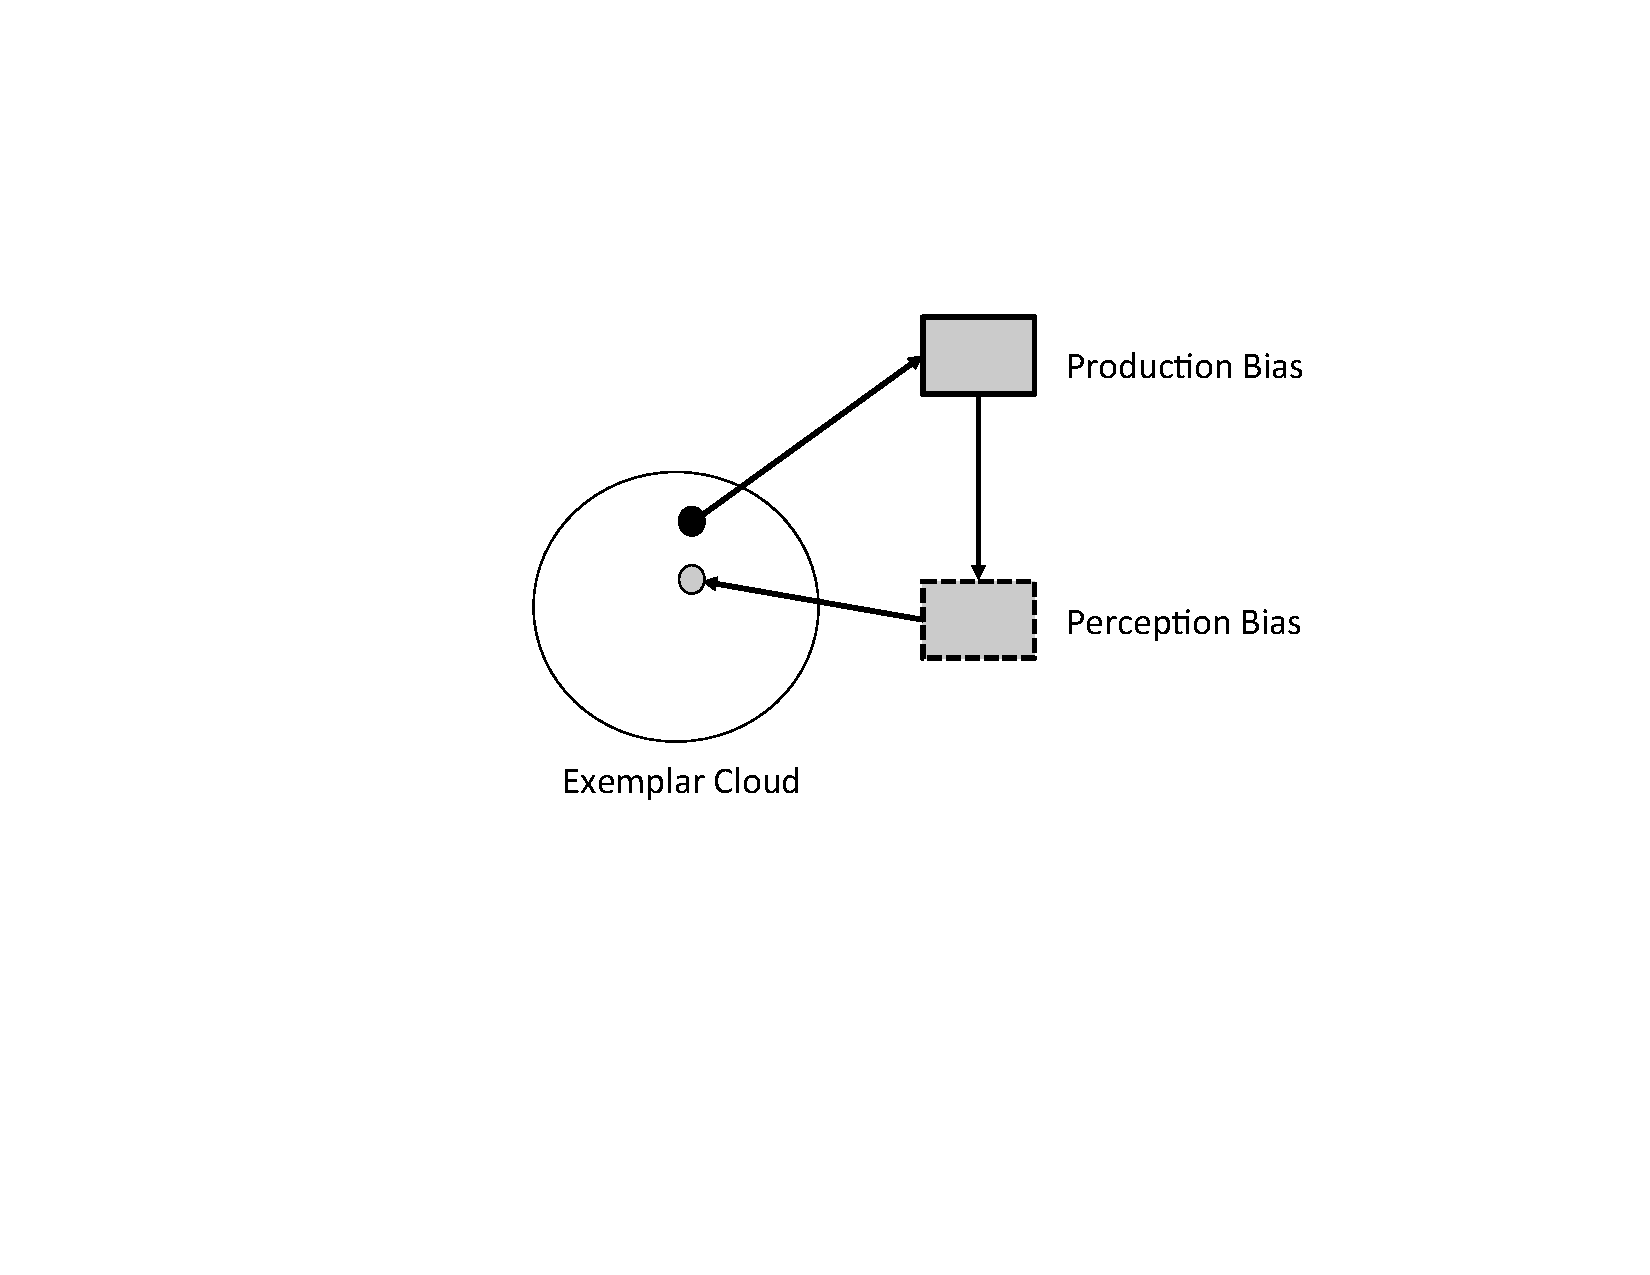
\includegraphics[scale=0.5]{figures/P-PLoop.pdf}\caption{\label{fig:Feedback Loop}Perception-Production Feedback Loop}
\par\end{centering}
\end{figure}

The basic \isi{exemplar} model includes three additional mechanisms that
are necessary for generating useful results. The first of these is
what is typically conceptualized as an error term. This allows for
variation to persist, and provides the necessary stochastic element
needed for achieving multiple outcomes. The second is \isi{entrenchment},
which prevents categories from losing cohesion and dispersing along
the dimensions of variation. The third mechanism is \isi{memory decay},
privileging more recent perceptions in memory, and preventing the
category from simply getting larger and larger. \figref{fig:Baseline-Model-Specification}
is a schematic of the basic algorithm for the models that will be
implemented and run below. Mathematical details will be provided in
the following section and the Appendices. 

\begin{figure}
\noindent\fbox{\begin{minipage}[t]{1\columnwidth - 2\fboxsep - 2\fboxrule}%
Baseline Perception-Production Model (one dimensional)
\begin{enumerate}[label=(\alph*)]
\item Initialize cloud
\begin{itemize}
\item assign values to a cloud of \emph{n} tokens (randomly generated from
a normal distribution of mean $\mu$ and variance $\sigma^{2}$)
\item assign each token an age (a time at which it was produced)
\end{itemize}
\item \label{enu:step 2}Randomly select a token for \isi{production}
\begin{itemize}
\item add the \isi{production} \isi{bias}, moving the token a small amount in the biasing
direction
\item add the error term, moving the token a small amount in either direction
\item add \isi{entrenchment}, moving the token a small amount closer to the category
mean 
\end{itemize}
\item Store
\begin{itemize}
\item add the new token value to the cloud
\item remove one of the oldest tokens from the cloud
\end{itemize}
\item Return to Step \ref{enu:step 2}
\end{enumerate}
\end{minipage}}
\caption{\label{fig:Baseline-Model-Specification}Baseline Model Specification}
\end{figure}


\section{Entrenchment}

Category consolidation, or variance reduction, has been motivated
as an effect of practice, or motor tuning (e.g. \citealp{saltzman1989dynamical}).
Implementationally, it is necessary to prevent the category expansion
in both directions that would result from consistent \isi{production} error,
and the additional expansion that would occur in the biasing direction.
The general equation for \isi{entrenchment} that will be used in this paper
is the following (based on \citealt{Pierrehumbert2000}):
\begin{equation}
E(x_{i})=\epsilon(\bar{x}-x_{i})\label{eq:Entrenchment}
\end{equation}
where $\epsilon$ is a constant between 0 and 1, $x_{i}$ is the current
location of token \emph{i} along some dimension \emph{x}, and $\overline{x}$
is the current category mean along that dimension. Figure \ref{fig:First Model param}
illustrates the evolution of a single \isi{exemplar} cloud generated from
the model outlined in \figref{fig:Baseline-Model-Specification}. In
each sub-figure the different colors indicate the same distribution
at initialization (white), and after a certain fixed number of model
iterations (black). Unless otherwise stated, all models are assumed
to be one-dimensional along \emph{x}. Individual tokens are given
as counts over successively binned \emph{x} values. 

\figref{fig:Basic-Iterative-Model} shows how the distribution as
a whole shifts in the direction of the \isi{production} \isi{bias} over time (measured
in iterations of the perception-\isi{production} loop). \figref{fig:NoEntrenchment}
shows the result of running the same model, minus the \isi{entrenchment}
term, over the same number of iterations. The biasing shift still
occurs, but with increasing variance along the biased dimension. See
Appendix \ref{chap:Appendix A} for the specific parameter values
used in these, and the following, simulations. 

\section{Memory decay}

Without \isi{memory decay}, categories can only spread without shifting.
The older the tokens, the more times, on average, they will have been
chosen as \isi{production} targets, reinforcing the initial conditions of
the cloud. Figure \ref{fig:No-memory-decay:} is an illustration of
this effect for the same model and starting conditions as the previous
two simulations, but with the \isi{memory decay} term removed. No tokens were
discarded. The skew in the direction of the \isi{production} \isi{bias} (implemented
as an incrementally decreasing function) can be seen in the left tail
of the distribution, but older tokens keep the category anchored at
the right. There are a number of ways in which a \isi{memory decay} term
can be implemented. In these and the following models, the total
number of tokens is kept constant by removing one of the oldest tokens
each time a new token is added.\footnote{There are other ways to keep the number of category members constant.
The token furthest from the mean could be discarded on each iteration,
for example. This would act to increase the \isi{entrenchment} effect, further
reducing variation. However, the purpose here is not only to keep
the number of tokens constant, but to allow a domino effect to develop
by increasing the probability that a token will be chosen again with
each biasing iteration. }

\begin{figure}[H]
    \begin{subfigure}[t]{.3\textwidth}
        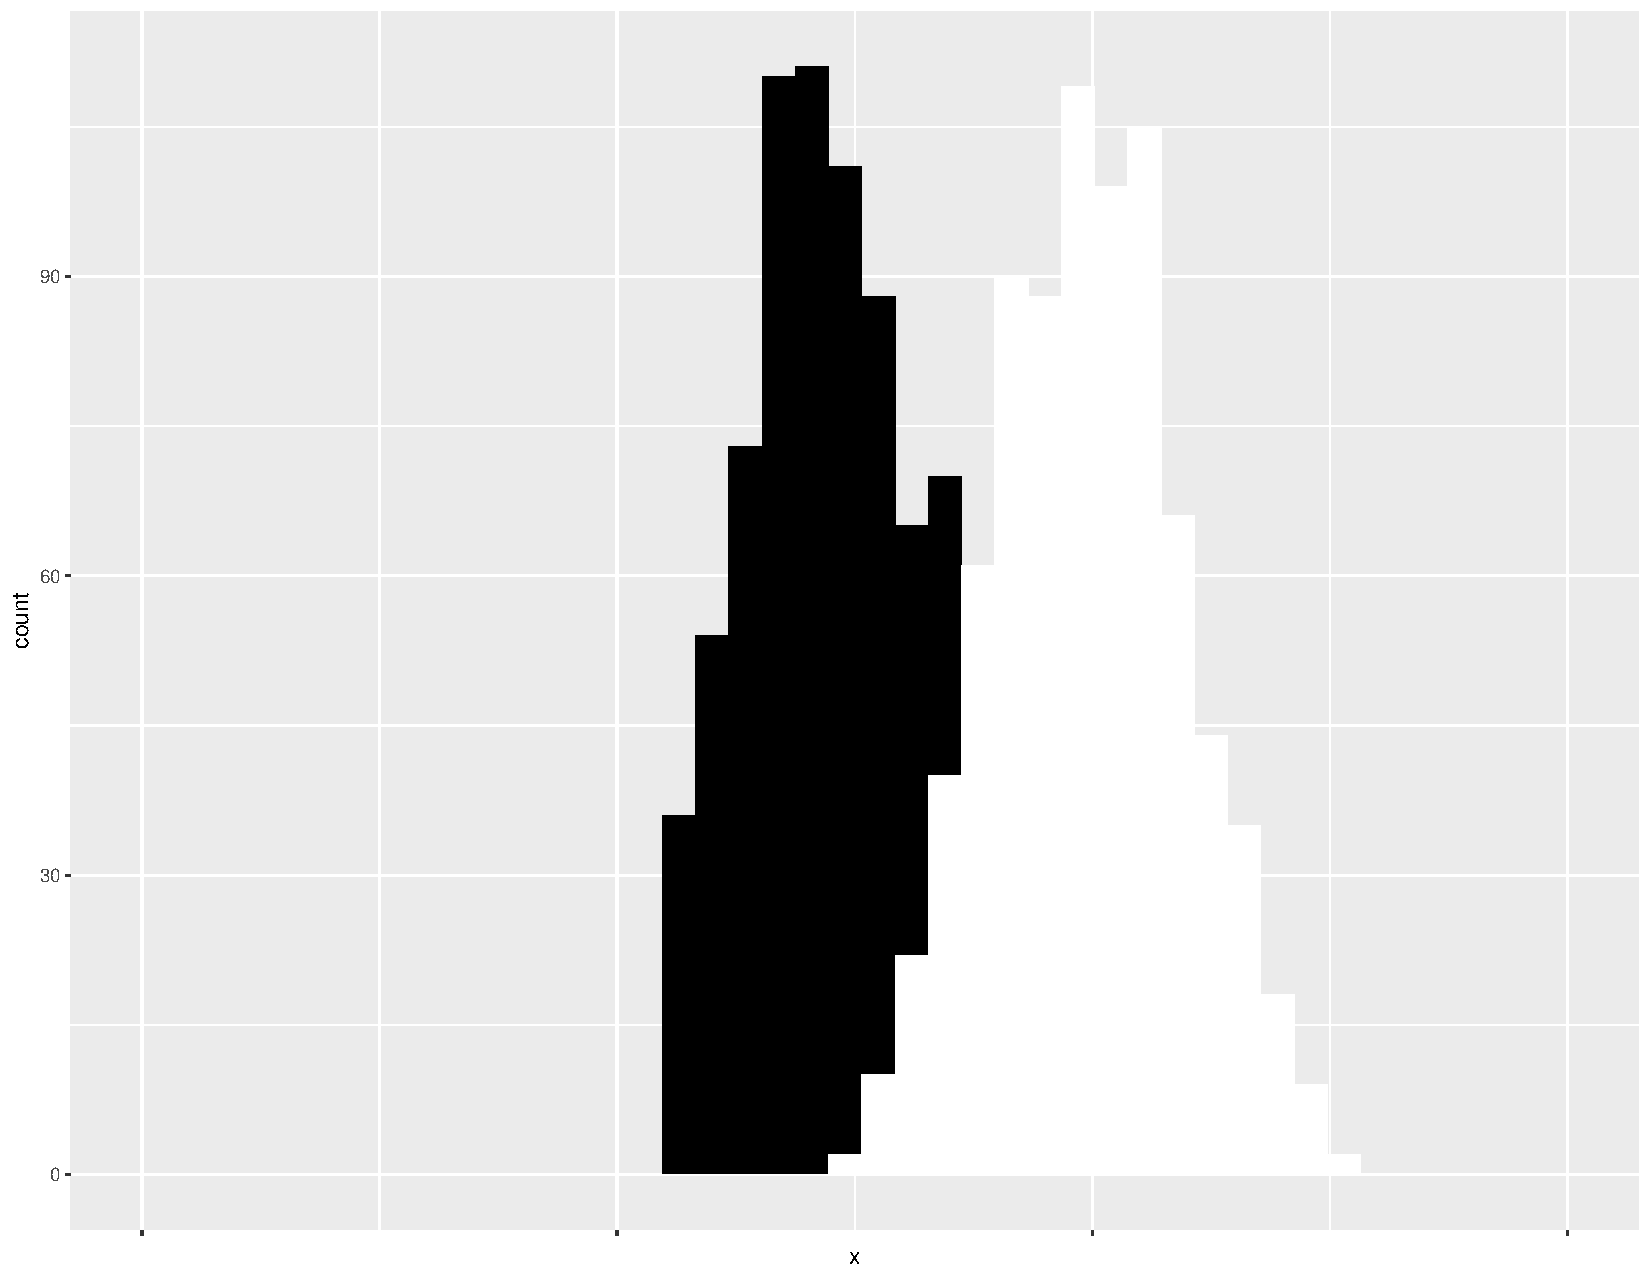
\includegraphics[width=\linewidth]{figures/8000iterwithentrenchment.pdf}
        \caption{\label{fig:Basic-Iterative-Model}All Forces}
    \end{subfigure}\hfill
    \begin{subfigure}[t]{.3\textwidth}
        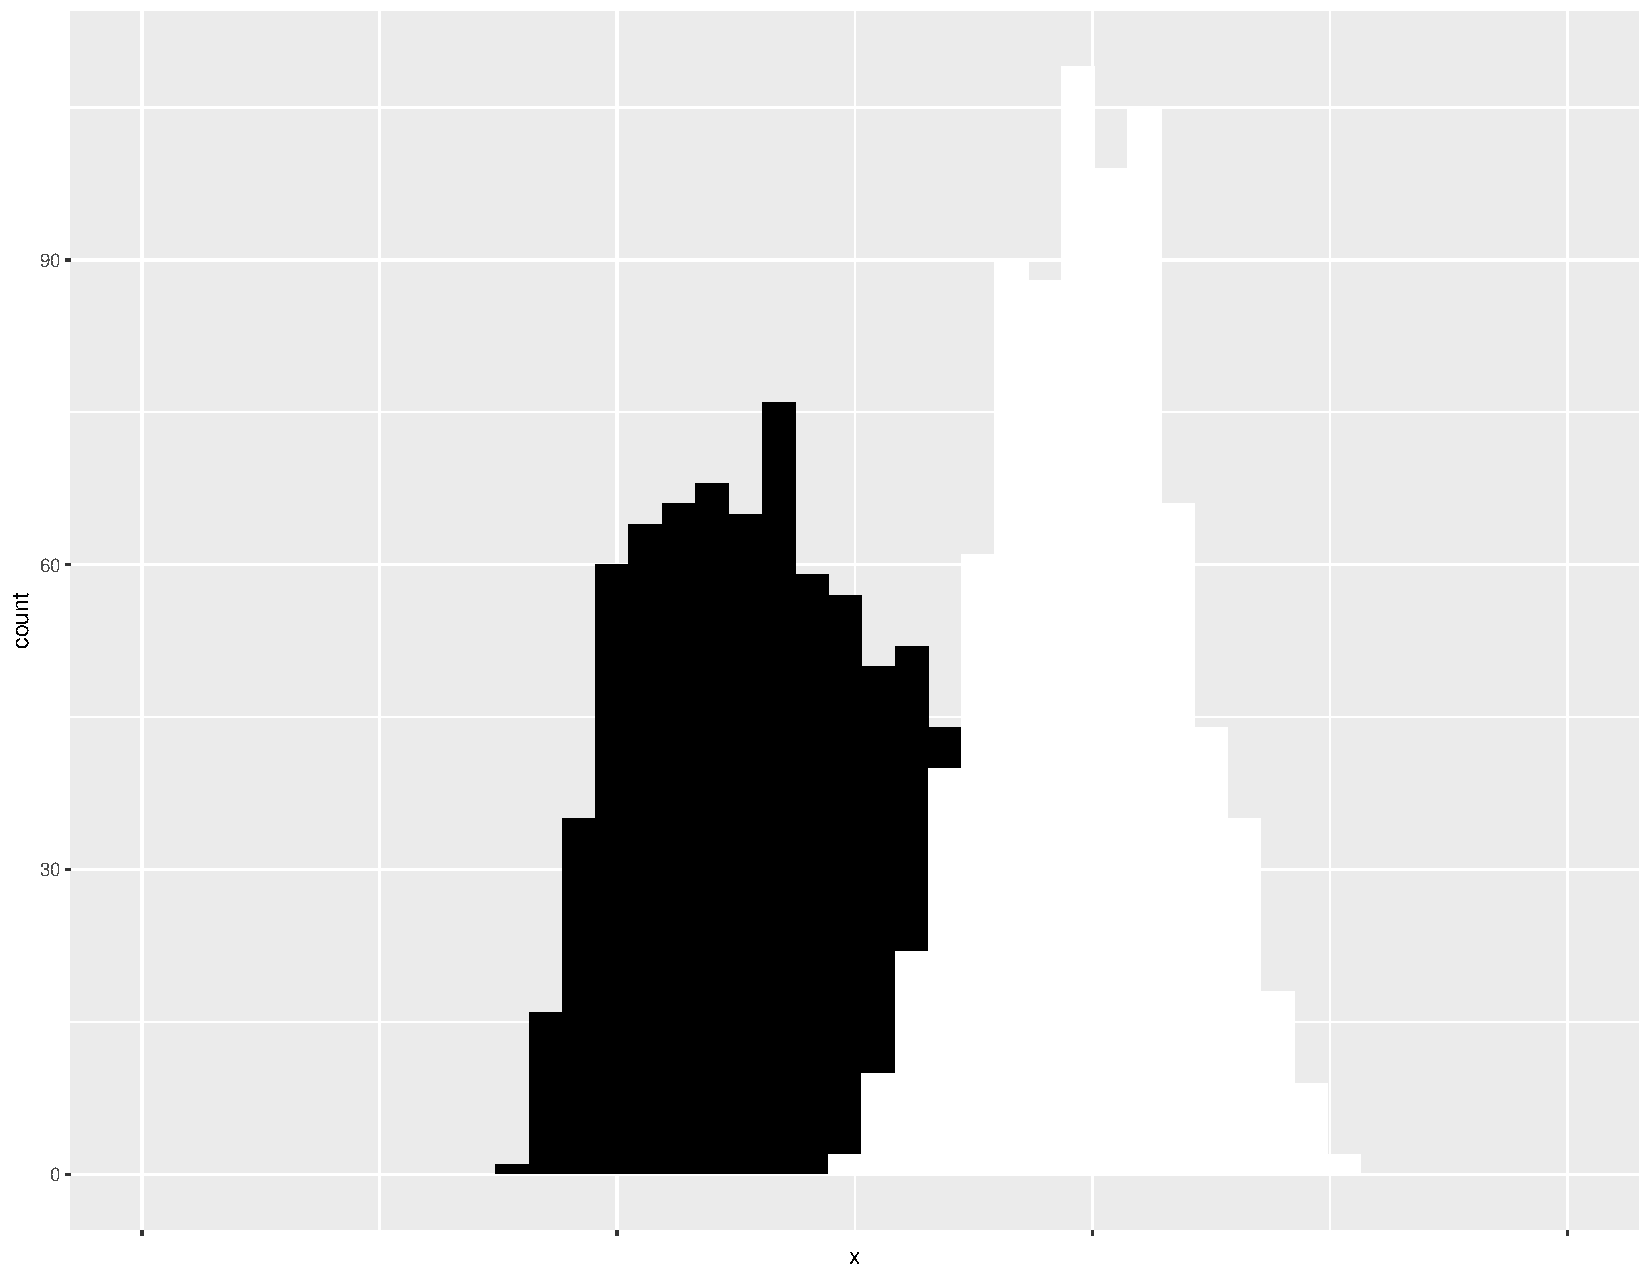
\includegraphics[width=\linewidth]{figures/8000iternoentrenchment.pdf}
        \caption{\label{fig:NoEntrenchment}Without Entrenchment}
    \end{subfigure}\hfill
    \begin{subfigure}[t]{.3\textwidth}
        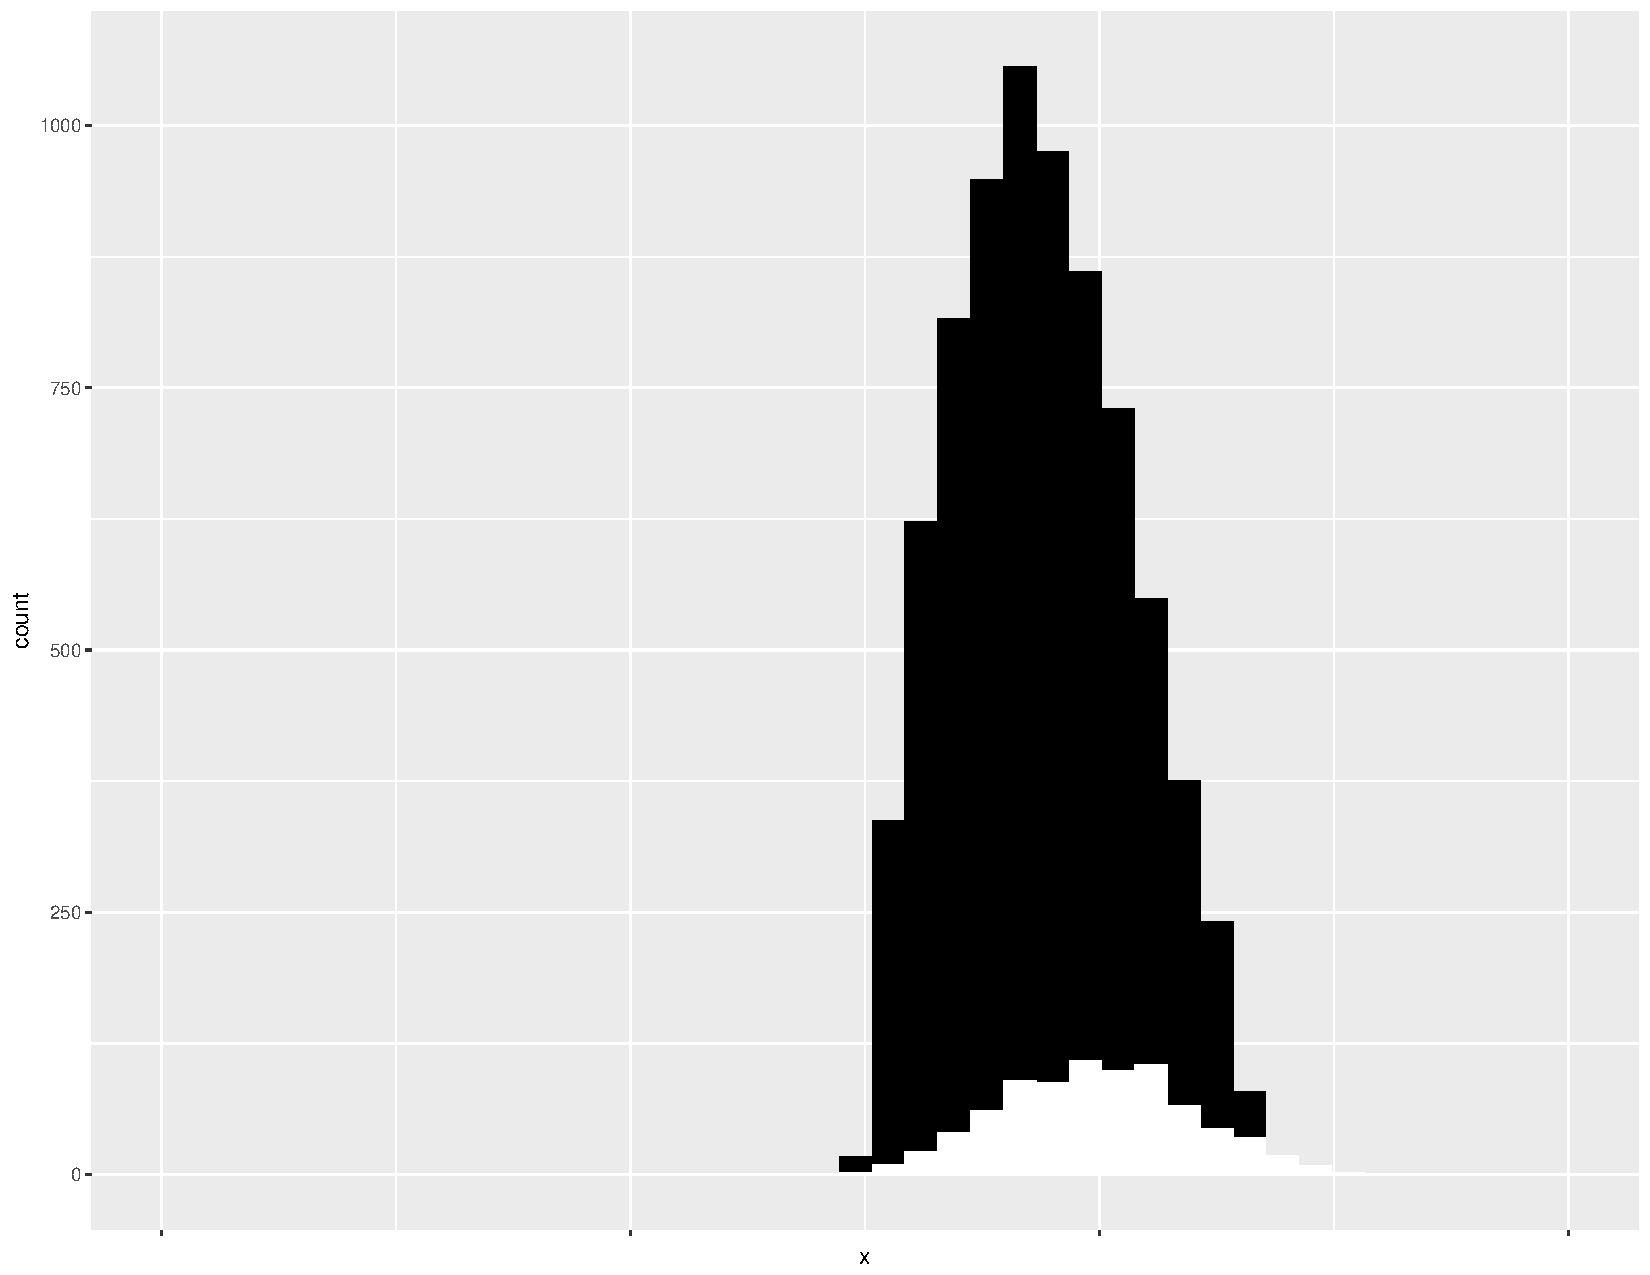
\includegraphics[width=\linewidth]{figures/8000iternomemory.pdf}
        \caption{\label{fig:No-memory-decay:}Without Memory Decay}
    \end{subfigure}
% % % \subfigure[\label{fig:Basic-Iterative-Model}All Forces]{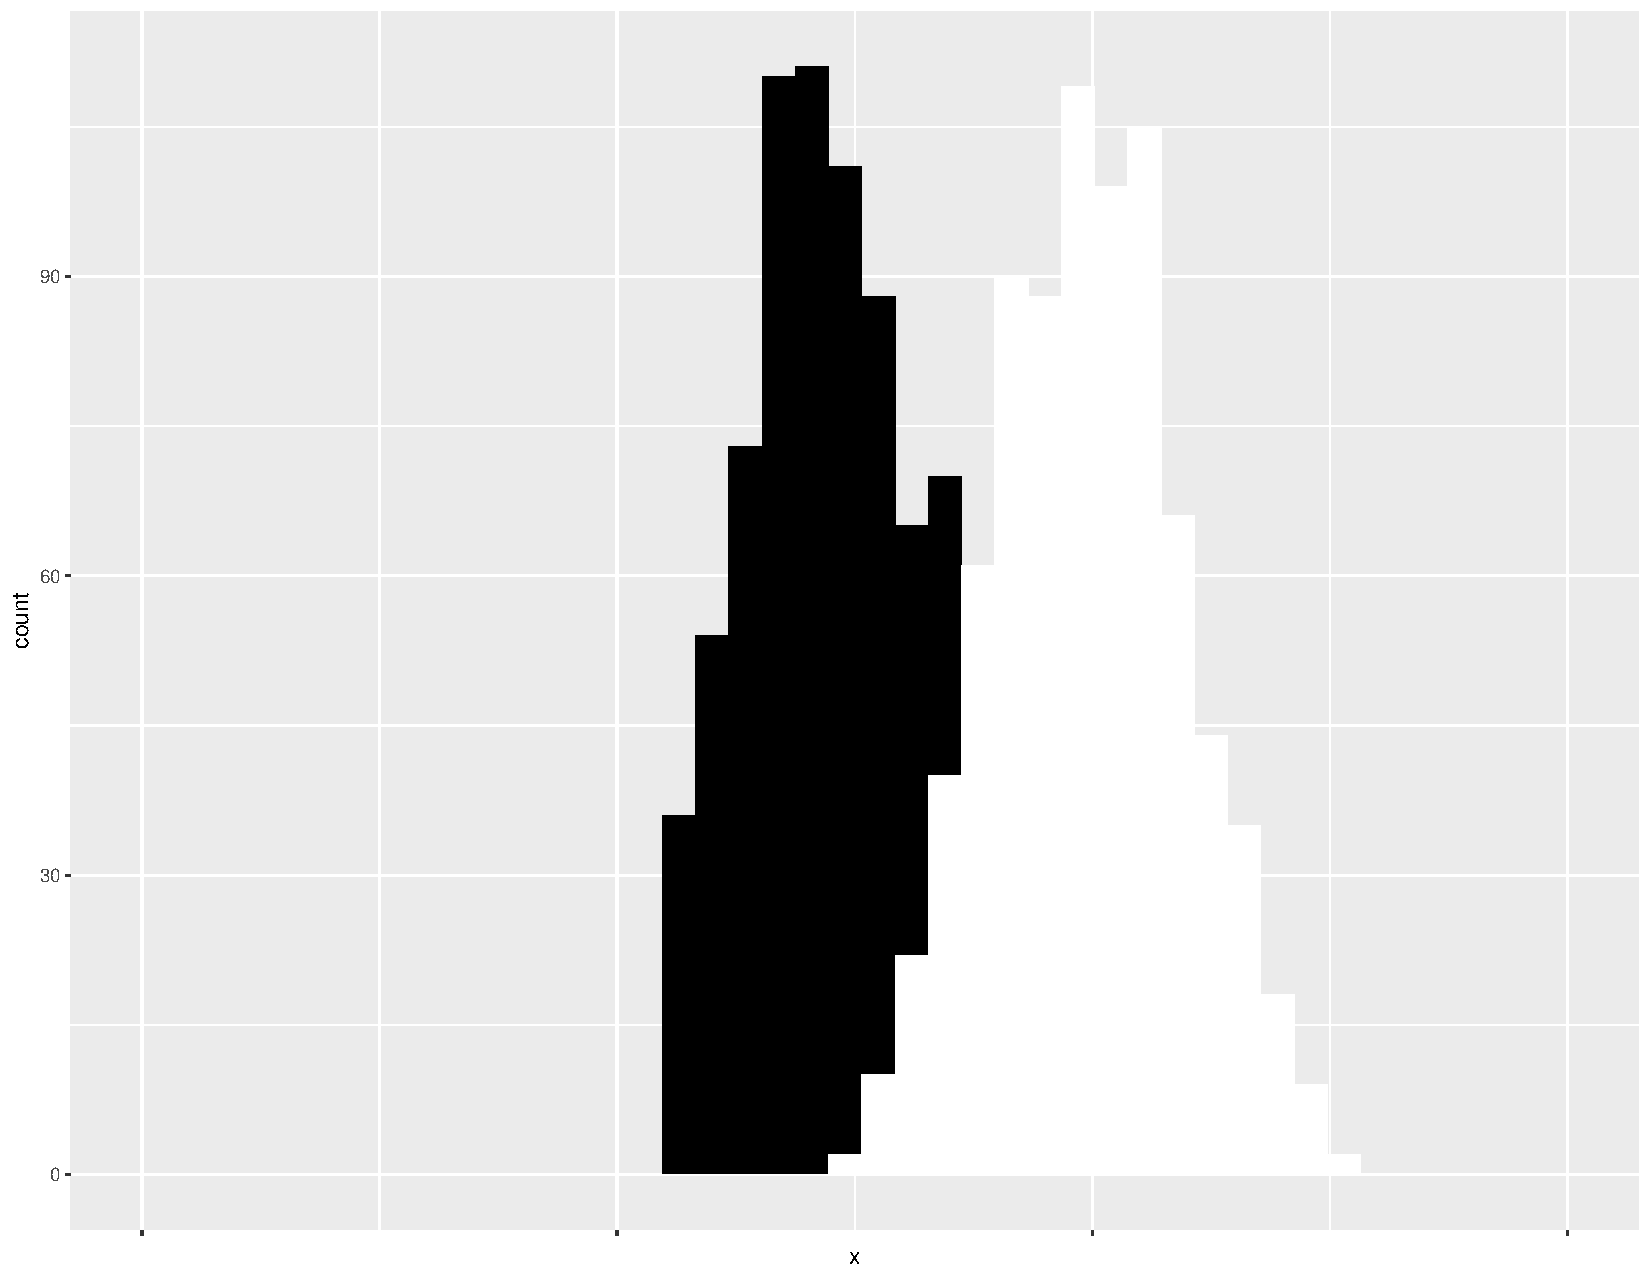
\includegraphics[width=0.25\textwidth]{figures/8000iterwithentrenchment.pdf}}\qquad
% % % \subfigure[\label{fig:NoEntrenchment}Without Entrenchment]{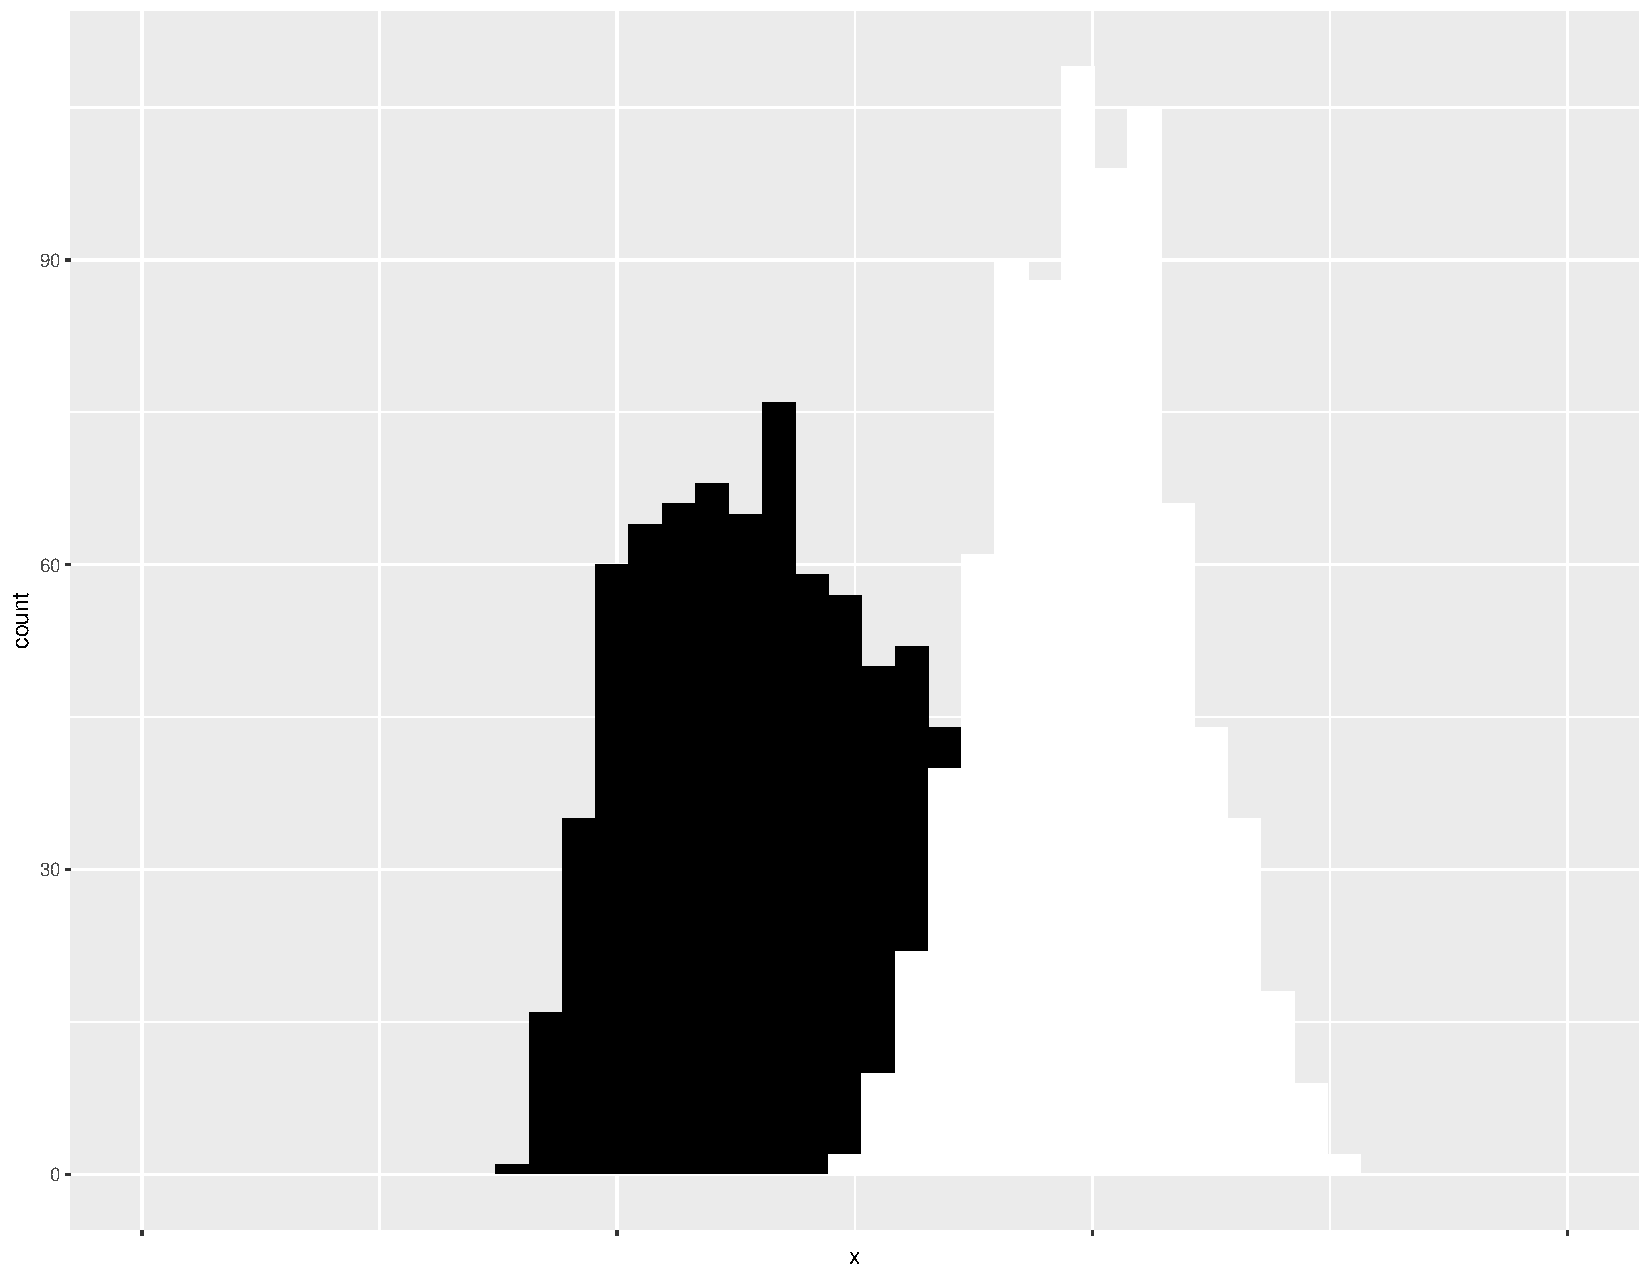
\includegraphics[width=0.25\textwidth]{figures/8000iternoentrenchment.pdf}}\qquad
% % % \subfigure[\label{fig:No-memory-decay:}Without Memory Decay]{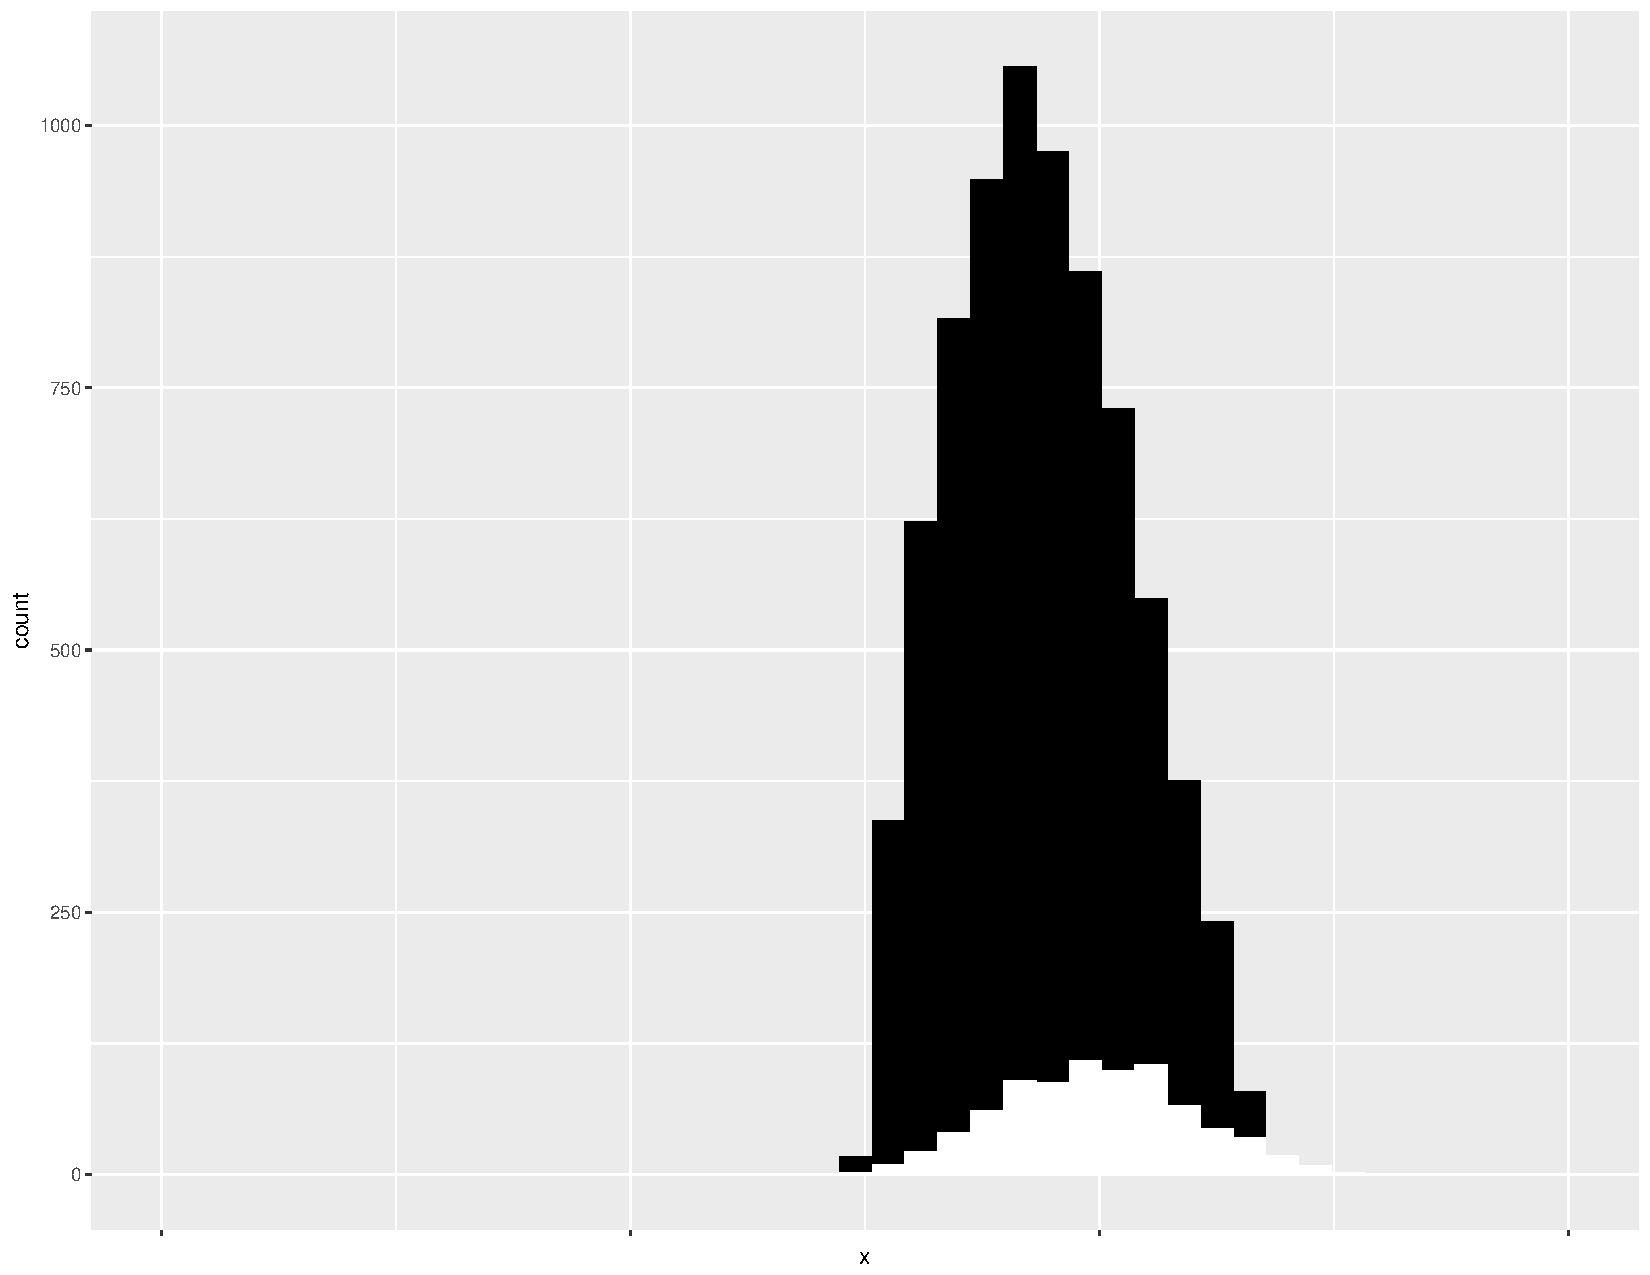
\includegraphics[width=0.25\textwidth]{figures/8000iternomemory.pdf}}
\caption{\label{fig:First Model param}Basic Iterative Model: Starting distribution
(white); Distribution after 8000 iterations (black). Note that y-axis
range in c) is about 10 times larger than in a) and b).}
\end{figure}


\section{\label{sec:Iterativity}The collapse problem}

As illustrated in \figref{fig:Basic-Iterative-Model}, the basic
\isi{exemplar} model with a single unidirectional \isi{bias} can produce cohesive
movement of an entire cloud of exemplars in the direction of the \isi{bias}.
What will be demonstrated in this section is that this shift is unbounded,
leading ultimately to category collapse and merger. This could easily
be inferred from the fact that the basic model contains only one force
that acts in a consistent direction, with nothing to oppose it. However,
it is worthwhile to actually run the simulations for a number of reasons.
Unambiguously establishing the results for general classes of phenomena
will allow us to see immediately what the model predicts for the linguistic
phenomena that map to each of those classes. Running actual simulations
will also force us to consider the question of whether \isi{exemplar} models
are to be evaluated only at convergence, and what the relationship
is between model time and real time, in terms of experiences of instances
of speech. Finally, the specific ways in which the models fail will
be informative regarding the mental representations they are meant to instantiate.

The three classes of phenomena to be modeled in this section are the
following: a context-free process; and two context-dependent processes, 
one gradient, and one categorical. For all of the three basic models,
a \isi{production} \isi{bias}, \emph{B}, will be implemented for a given token
\emph{i}, as a fixed percentage reduction ($\alpha$) in the value
of \emph{$x_{i}$} along dimension \emph{x}. See Eq. (\ref{eq:Production Bias}).\footnote{The \isi{production} \isi{bias} in \citet{Pierrehumbert2000} is a constant that
applies regardless of the current token value. Making the \isi{bias} proportional
results in less reduction for tokens that already have small values, thus
fixing the percentage of reduction, rather than the absolute value,
for all tokens.} 
\begin{equation}
B(x_{i})=-x_{i}\alpha\label{eq:Production Bias}
\end{equation}
After the \isi{production} \isi{bias} applies, the biased token will be added
back to the cloud from which it was originally drawn. It will be useful
to express the value of a given token on any iteration as a function
of the original non-biased token that gave rise to it. For one such
original token, $x_{i}$, we can label its biased daughter as $x_{i(+1)}$,
and calculate its biased value to be $x_{i}(1-\alpha)$
along dimension \emph{x}. If, on some subsequent iteration, this daughter
token $x_{i(+1)}$ is chosen for \isi{production}, it will be subject to
the same biasing force, resulting in the granddaughter, $x_{i(+2)}$,
with value $x_{i(+2)}=x_{i(+1)}(1-\alpha)=x_{i}(1-\alpha)^{2}$.
Proceeding to the general case, we can express the value of any token,
on any given model iteration, as a function of the value of its originator
token ($x_{o}$), and the number of generations, \emph{n}, by which
the current token is removed from that originator. See Eq. (\ref{eq:linear bias}). 
\begin{equation}
x_{o(+n)}=x_{o}\left(1-\alpha\right)^{n}\label{eq:linear bias}
\end{equation}


\subsection{\label{subsec:Model-1:-Context-Free}Model 1: Context-free iterativity}

In Model 1, the \isi{bias} function applies to all tokens. Therefore, the
linear \isi{bias} term in (\ref{eq:linear bias}) will cause the entire
category to shift in the biasing direction over time. The following
simulations compare the behavior of a low-\isi{frequency} category, to a
high-\isi{frequency} category, one whose tokens are produced, and thus experienced,
more often. All simulations begin with the same starting distributions:
a high-\isi{frequency} category with 800 tokens, and a low-\isi{frequency} category
with 200 tokens. Steps were taken to make the distributions of the
two categories as close as possible.\footnote{The high-\isi{frequency} category was generated by randomly sampling 800
tokens from a normal distribution with mean of $50x$ and a standard
deviation of $2x$. The low-\isi{frequency} category was then created by
sampling 200 tokens from the high-\isi{frequency} category: 50 tokens from
each quartile.} See Figure \ref{fig:Frequency Starting Dist}. 

\begin{figure}[H]
\centering{}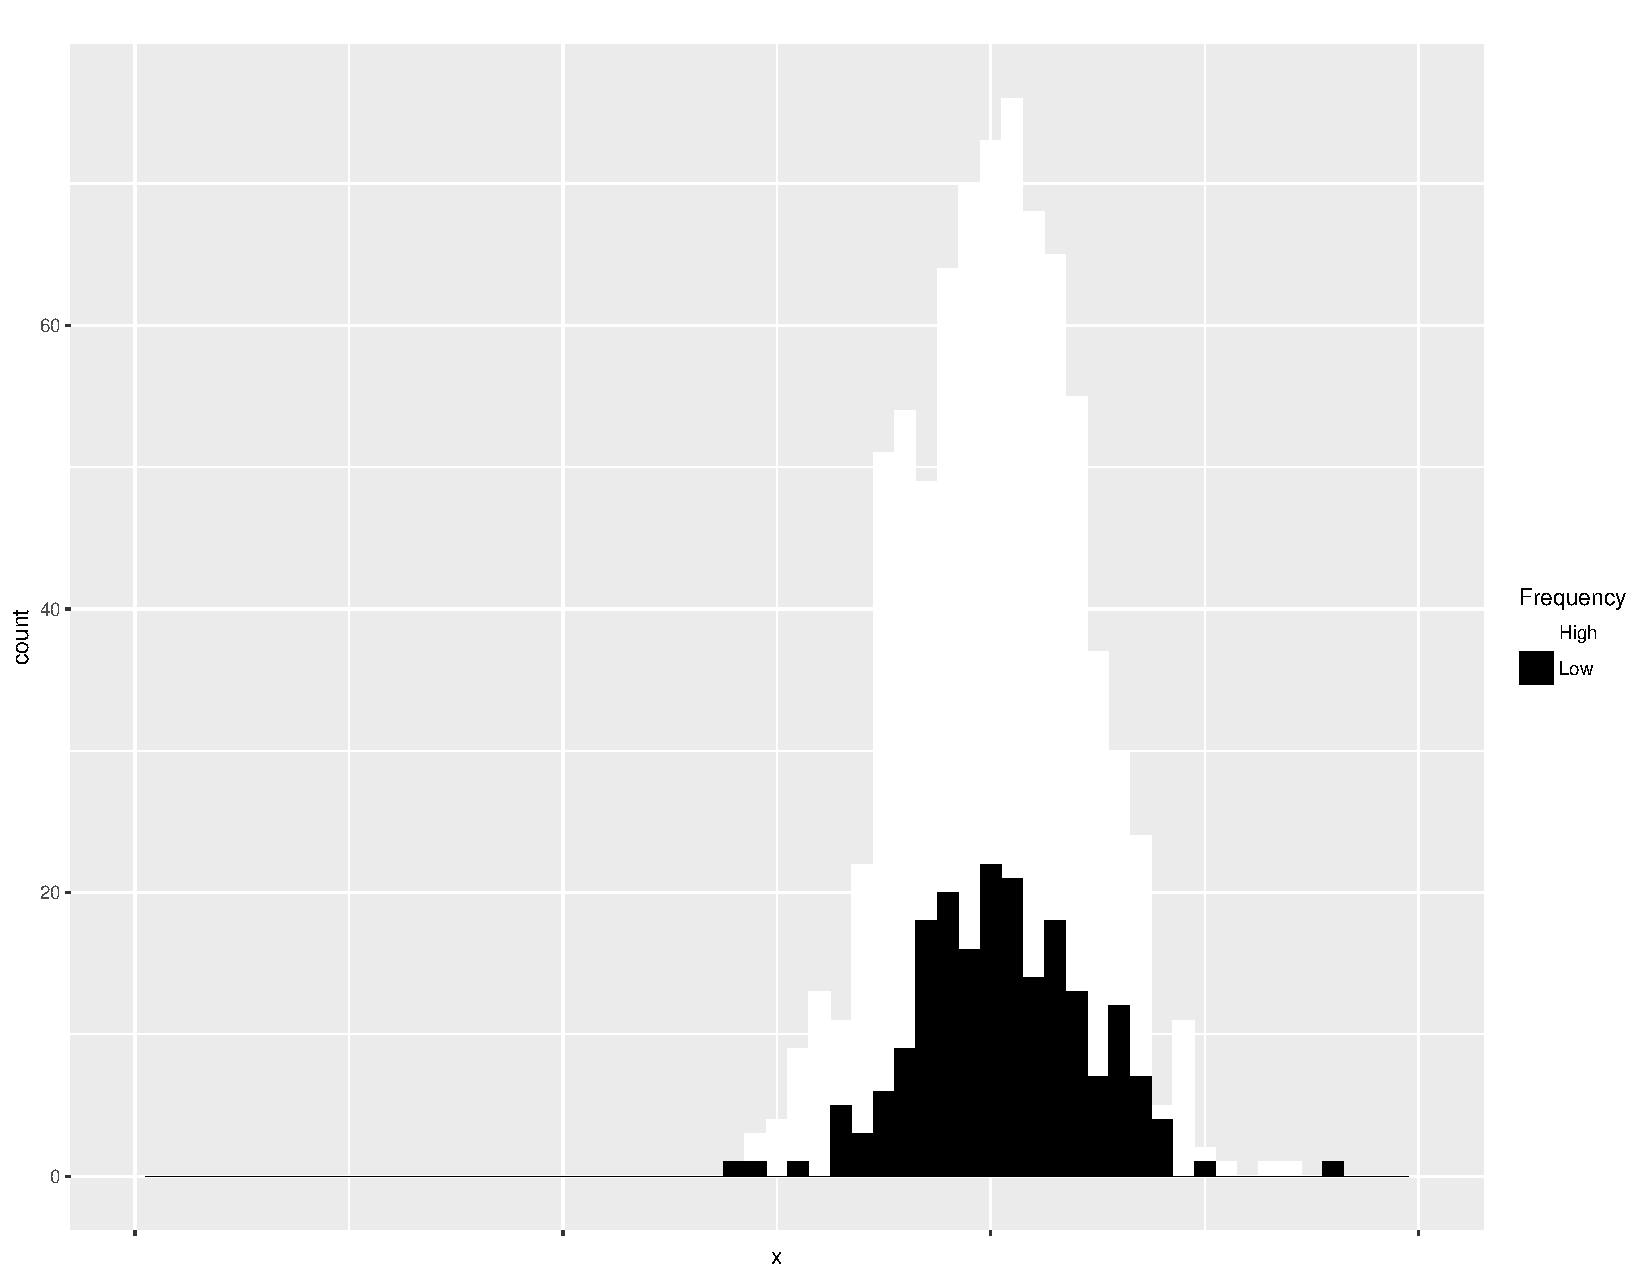
\includegraphics[scale=0.25]{figures/startCon.pdf}\caption{\label{fig:Frequency Starting Dist}Starting Distribution. White bars:
High-frequency category. Black bars: Low-frequency category.}
\end{figure}

Because these models rely on random processes, the outcome is not
guaranteed to be identical each time the model is run. To evaluate
models of this kind, one conducts a number of independent identical
``experiments'' (trials) that consist of running the model with the
same starting conditions, and the same parameters, for the same number
of iterations. Results are then averaged over the set of trials. In
the first set of simulations, 500 model trials were run for 1000 iterations
each. On each model iteration one token was produced, selected stochastically
from among all possible tokens (making it 4 times more likely to be
chosen from the high-\isi{frequency} than the low-\isi{frequency} category). That
token was biased according to Eq. (\ref{eq:Production Bias}) and
then added back to the category from which it originated. 

The mean category value along \emph{x} for each category was calculated
at the end of each of the 500 trials, and converted to a z-score.
A boxplot of the difference between the means of the two categories
on each trial is shown in \figref{fig:HvL}. In 44\% of trials the
difference was negative (low-\isi{frequency} mean larger than high-\isi{frequency}),
and in 56\% it was positive. The mean difference over all 500 trials
was close to zero: 0.031 (or 16\% of the initial distribution standard
deviation). Thus we do not see a consistent difference in the two
categories after an arbitrarily selected number of iterations. Intuitively,
we might have expected the higher-\isi{frequency} category to have moved
further along \emph{x}, and have a lower value, because tokens from
that category are produced more often, and thus multiply-biased.
However, it is also the case that, if \isi{frequency} of occurrence is expressed
in number of tokens, and sampling for \isi{production} is random, then producing
a token that had undergone biasing \emph{fewer} times is also more
likely in high than in low \isi{frequency} categories. This is simply because
there are more tokens, which lowers the probability of selecting any
individual token, and thus lowers the probability of selecting the
daughter of any individual token, relative to the low-\isi{frequency} category. 

\begin{figure}[H]
\begin{subfigure}[t]{.45\textwidth}
        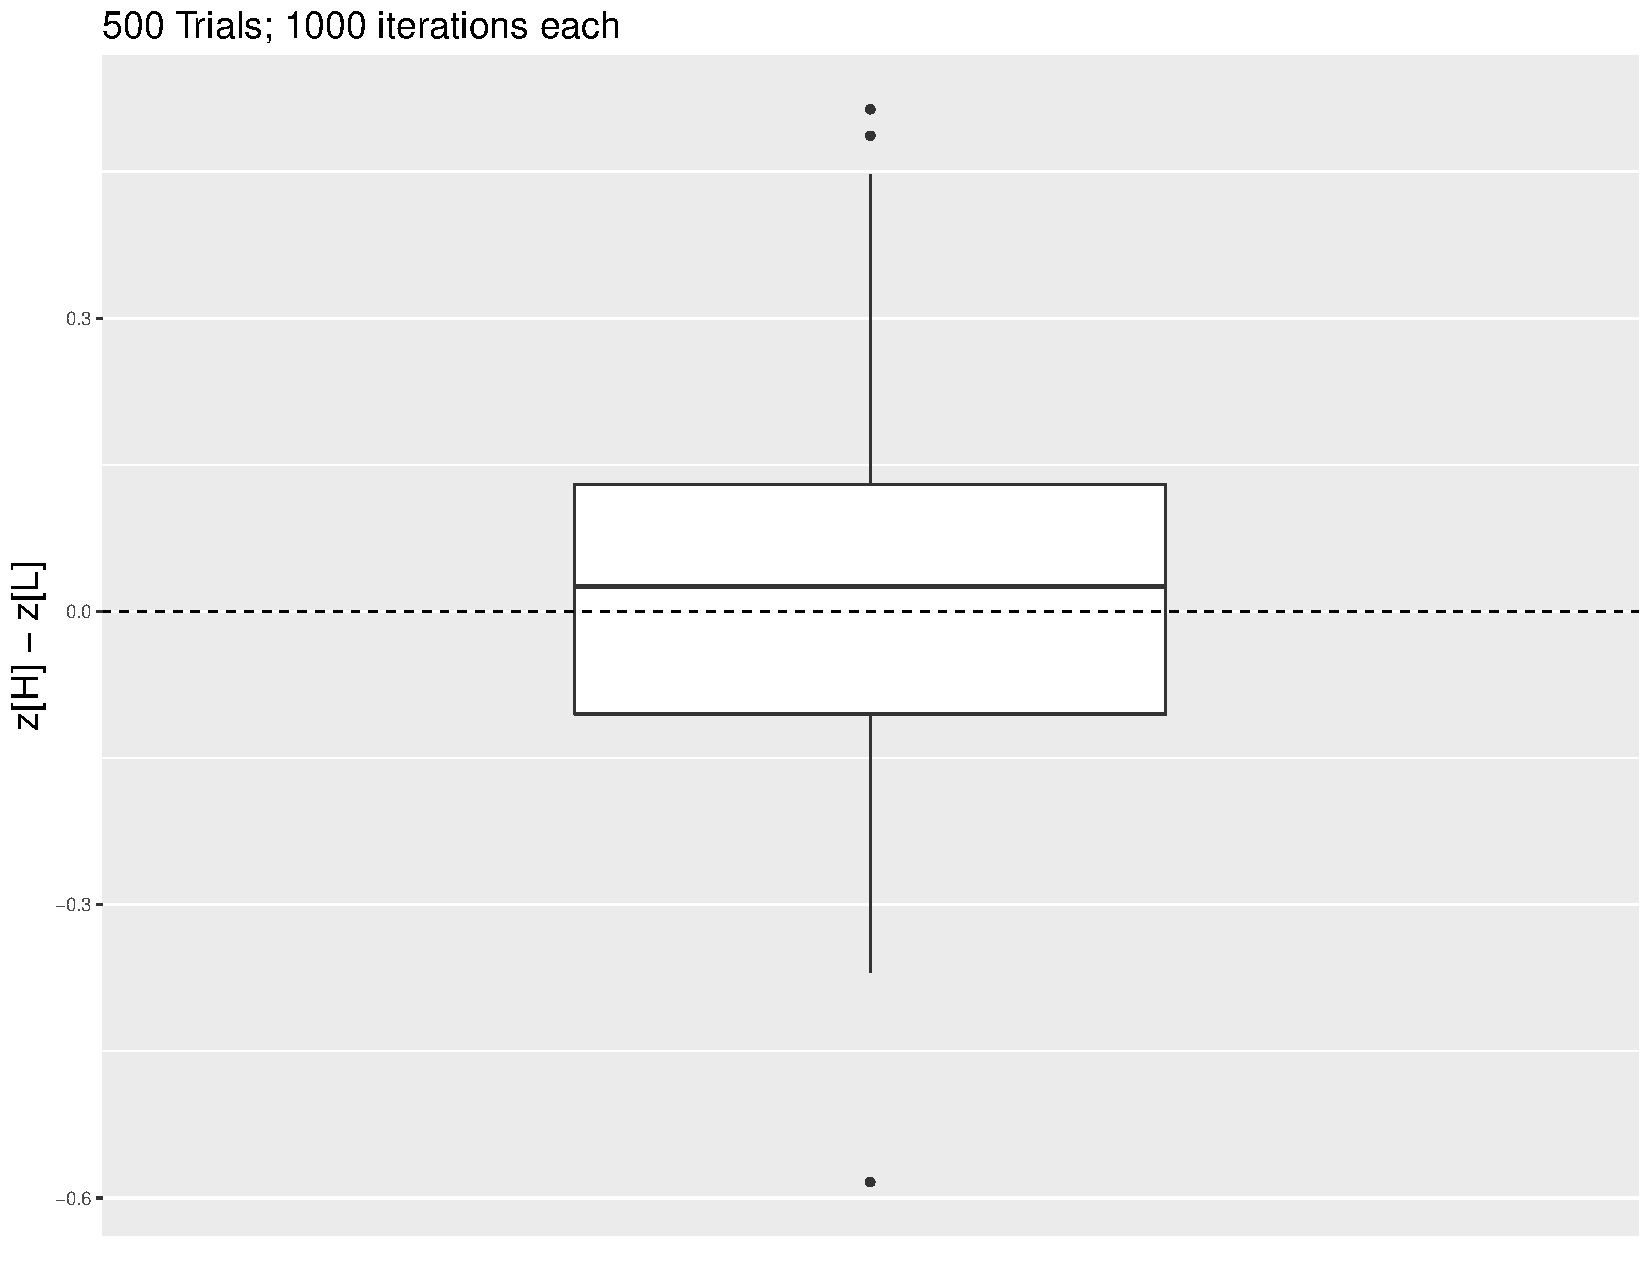
\includegraphics[width=\linewidth]{figures/FrequencyEffect.pdf}
        \caption{\label{fig:HvL}4:1 Token ratio}
    \end{subfigure}\hfill
    \begin{subfigure}[t]{.45\textwidth}
        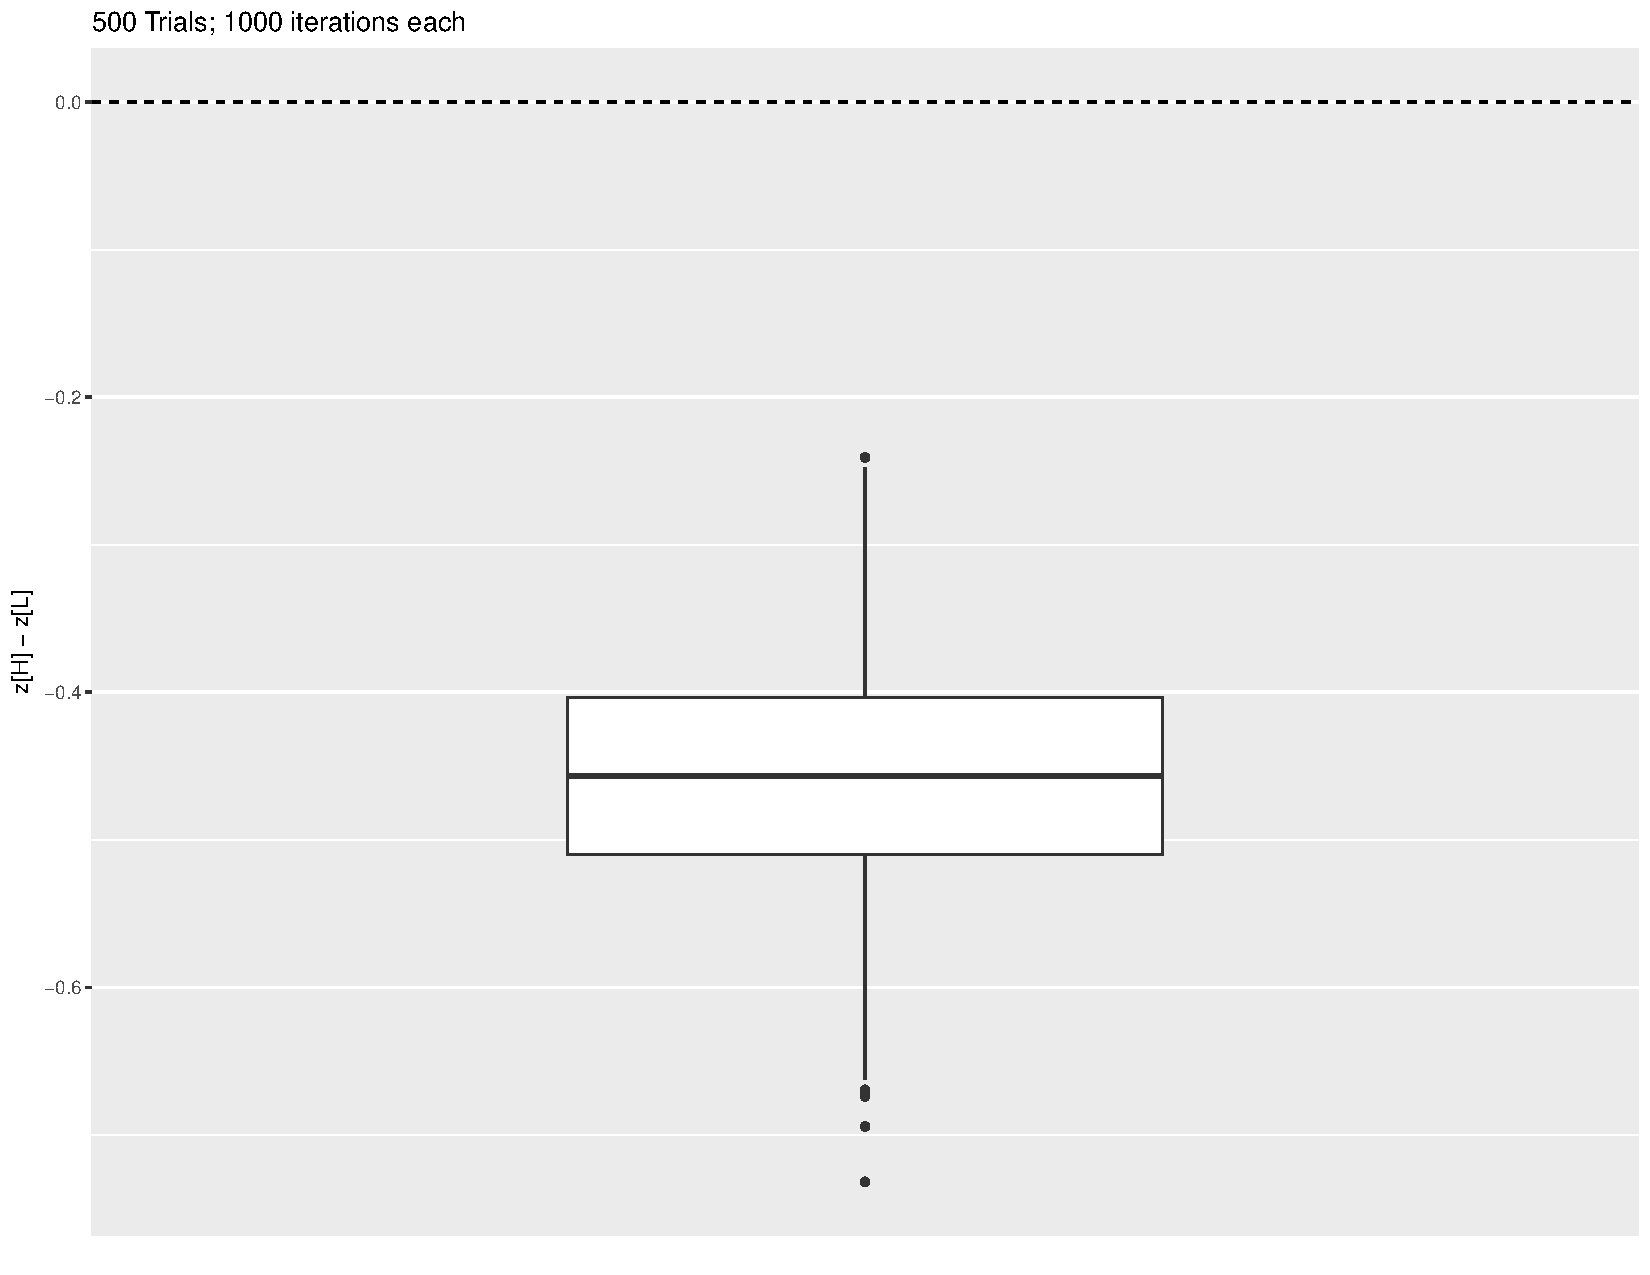
\includegraphics[width=\linewidth]{figures/FrequencyEffectEqNums.pdf}
        \caption{\label{fig:Freq.EqualTokens}1:1 Token Ratio}
    \end{subfigure}
% % \centering{}\subfloat[\label{fig:HvL}4:1 Token ratio]{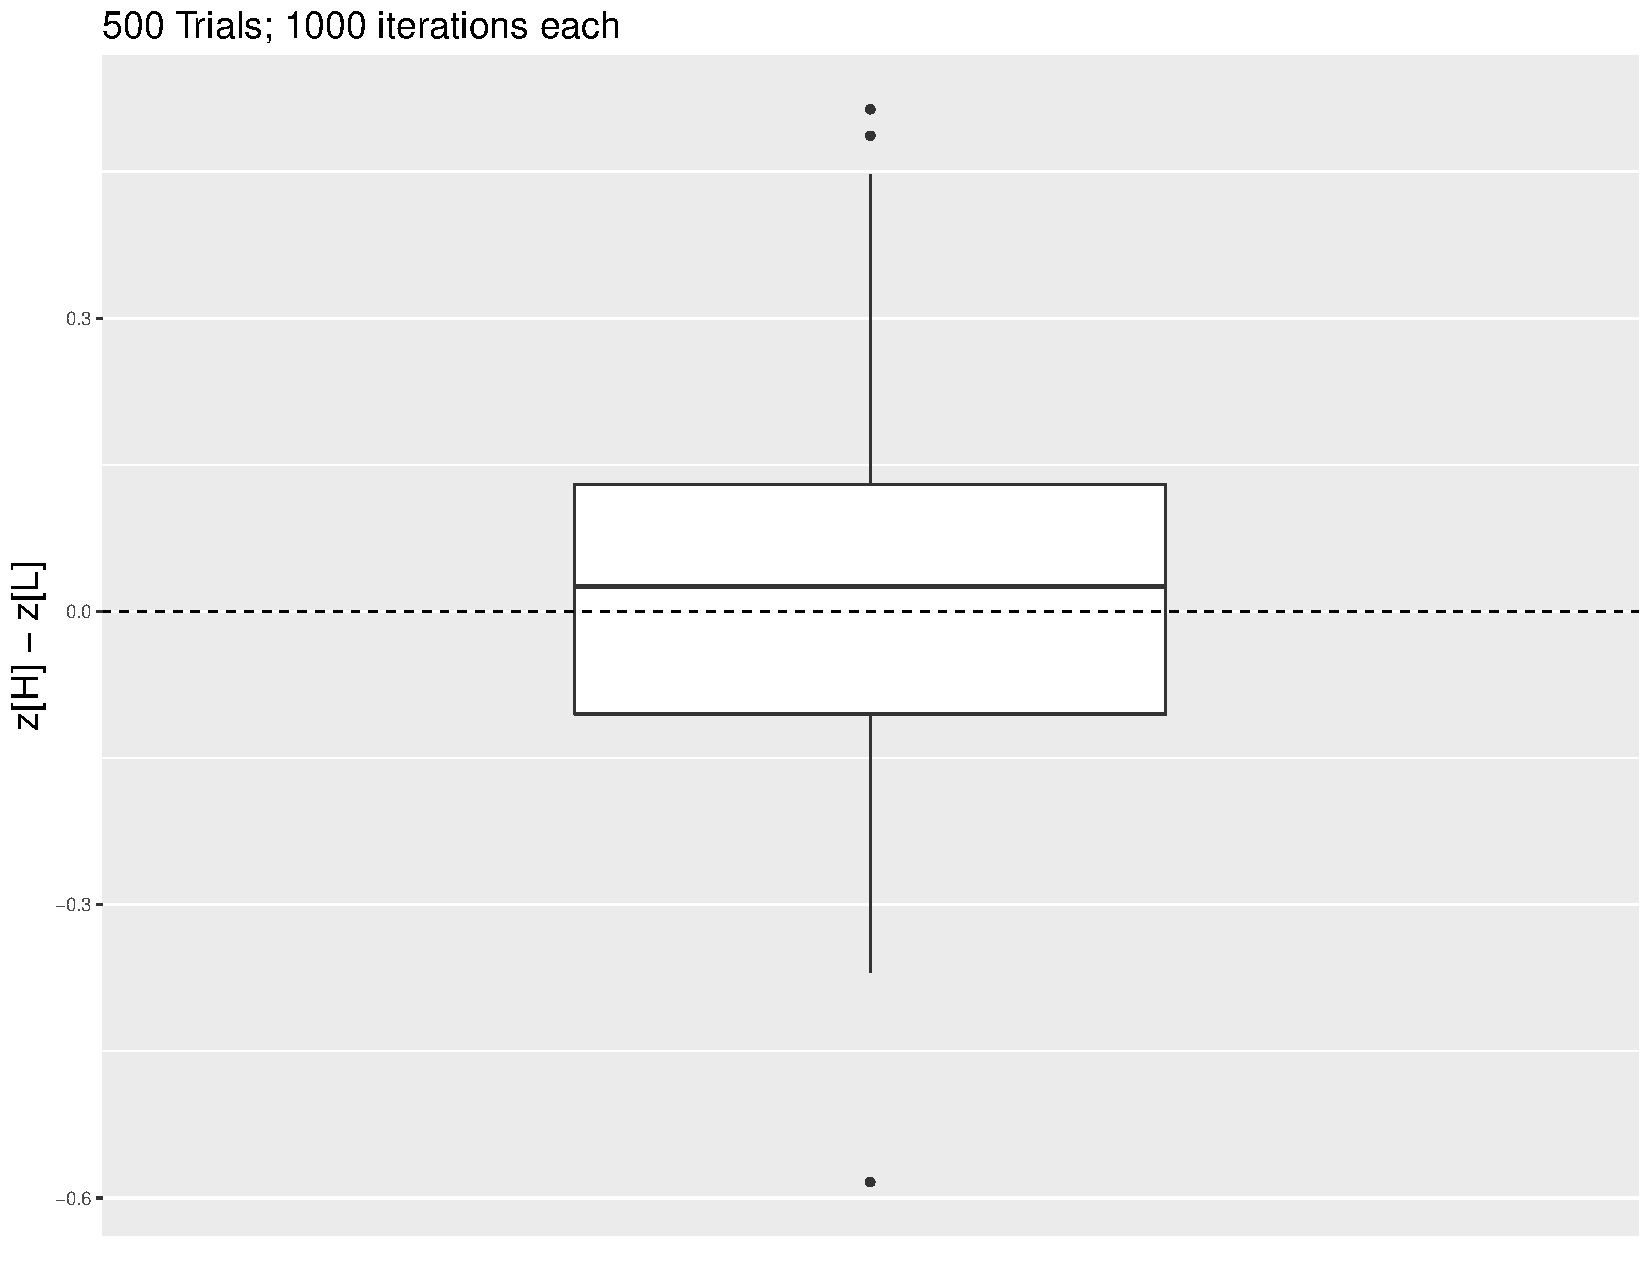
\includegraphics[width=0.3\textwidth]{figures/FrequencyEffect.pdf}}\hfill{}\subfloat[\label{fig:Freq.EqualTokens}1:1 Token Ratio]{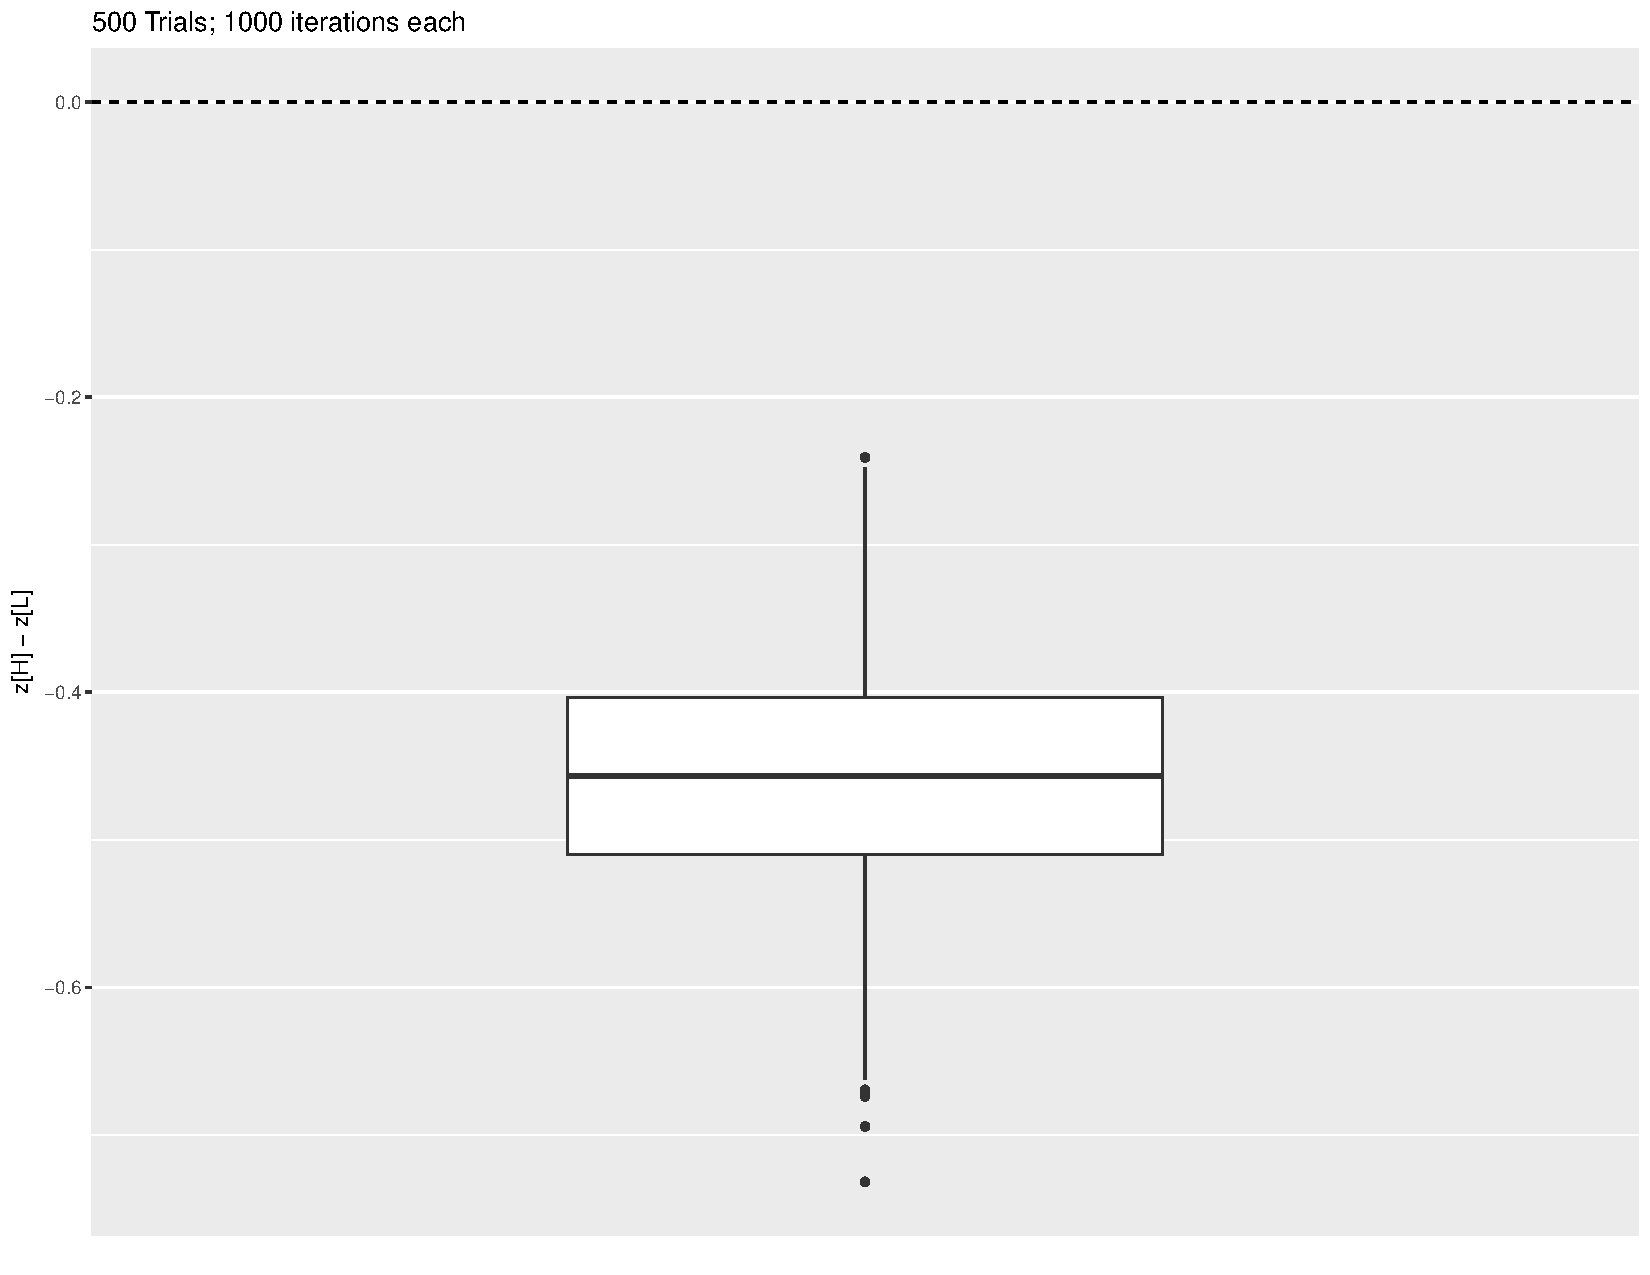
\includegraphics[width=0.3\textwidth]{figures/FrequencyEffectEqNums.pdf}}
\caption{Simulation of Iterative Biasing for H(igh) frequency category versus
L(ow) frequency category}
\end{figure}

The difference in the number of tokens in each category also results
in a difference in variance across the different trials. The variance
is larger for the lower-\isi{frequency} category due to undersampling; because
fewer tokens are produced from the low-\isi{frequency} category in a given
trial, and the tokens are selected randomly, the likelihood that the
sample will be significantly different from trial to trial is greater
(\citealt{Soskuthy} finds a similar effect using a parameterized \isi{exemplar}
model). Variance compounds over iterations, such that the variance
between independent model runs after 10,000 iterations is greater
than after 5000 iterations. \figref{fig:Frequency Catch Up} illustrates
the across-trial variance for the two categories at successive intervals,
after 500, 1000, 1500, and 2000 iterations.

\begin{figure}[H]
\centering{}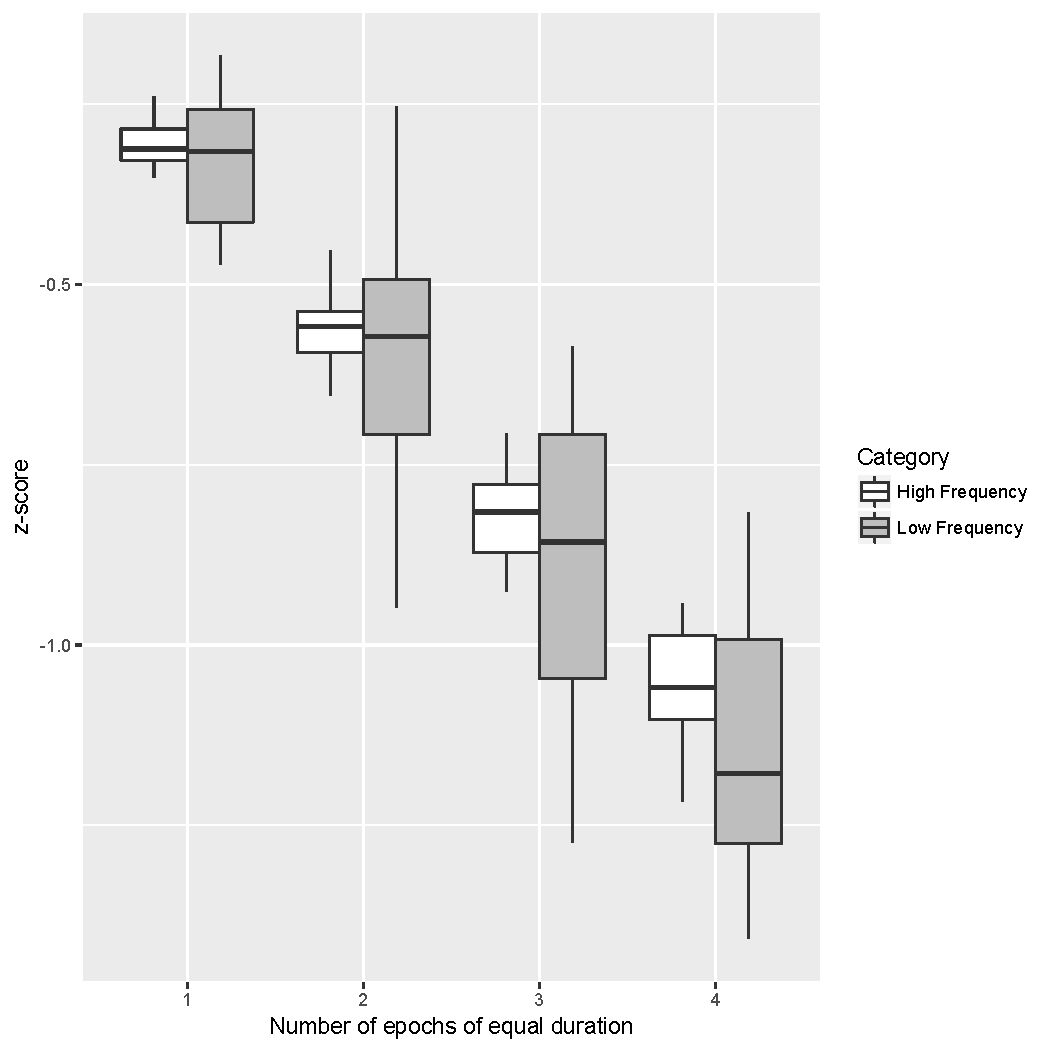
\includegraphics[width=.75\textwidth]{figures/FrequencyOverTime.pdf}\caption{\label{fig:Frequency Catch Up}Average z-scored value for High (white)
versus Low (gray) frequency categories at 4 equally spaced intervals
of model time, each 500 model iterations in duration (1 epoch). Each boxplot shows
the results of 10 independent trials at each of the successive epochs.}
\end{figure}

Different implementational choices and assumptions will produce somewhat
different results. If the two categories contain the same constant
number of tokens, but the high-\isi{frequency} category is still 4 times
more likely to be produced on any given iteration, then the high-\isi{frequency}
category will have a consistently lower value along \emph{x} than
the low-\isi{frequency} category. The results of the equal-tokens simulations are shown in \figref{fig:Freq.EqualTokens}.
This is because the \isi{inertia} from the larger number of few-times-biased
tokens is missing. These specific results also depend on the ratio
of frequencies of the two categories, as well as a number of other
parameter settings. Those dependencies will be discussed further in
Section \ref{subsec:Word-Frequency}, when this model is linked to
the linguistic phenomenon of frequency-based word reduction. For now,
we turn to the behavior of the model in the limit.

The means of both categories steadily decrease as a function of the
number of model iterations. Although the amount of biasing becomes
steadily smaller as token values become smaller, biasing is unbounded.
That is, the model does not converge on a stable state. Convergence
can be imposed by specifying a minimum value on \emph{x} beyond which
tokens cannot be reduced. This results in a skewed distribution with
a narrow peak at the threshold value and a small rightward tail due
to the normally distributed error term. The thresholded model clearly
illustrates that all categories, whether high or low \isi{frequency}, will
eventually end up at exactly the same minimum value, collapsing any
difference between them. 

\subsection{\label{sec:Context-Dependent-Iterativity}Context-dependent iterativity}

In the previous model all tokens of each category were subjected to
the same \isi{production} \isi{bias} – the context in which the tokens were produced
did not matter. The next two models are context-dependent models.
In these models the \isi{production} \isi{bias} only applies to a subset of tokens,
those produced in the biasing context. As before, \isi{production} tokens
are chosen at random; they are then produced in either a biasing or
non-biasing context, with a certain fixed probability. Regardless
of \isi{production} context, however, all tokens are added back to the same
originating category.

\subsubsection{\label{subsec:Phrase-Final Lengthening}Model 2: Gradient context-dependent bias}

Model 2 implements a gradient \isi{production} \isi{bias}, similar to the one
used in Model 1, but with an increasing, rather than decreasing, function
of $x$. On each iteration, the randomly selected token has probability
\emph{p} (< 0.5) of increasing by a fixed percentage ($\alpha$) of
its current value. As before, the category is initialized by sampling
from a normal distribution, and all tokens begin with non-biased values.
Because there is only one cloud in \isi{perception}, the only time a difference
between biased and non-biased tokens can be observed is at the moment
of \isi{production}. Therefore, model outputs will be given in terms of
an observed random sample of fixed size at some cycle, \emph{n}, of
the model.

The \isi{iterativity} of the perception-\isi{production} loop allows for tokens
to be biased multiple times, but also for tokens to remain persistently
non-biased, the more so the larger the category is in terms of stored
exemplars, and the smaller the value of \emph{p}. To understand model
behavior it is useful to think of each iteration as involving four
possible outcomes. In the first, a relatively low-valued token (the
outcome of a series of productions occurring more often in non-biasing
contexts) is chosen for \isi{production}, but this time in a biasing context,
thus increasing its value along \emph{x}. The second possibility is
that the same token is chosen for \isi{production} in a non-biasing context,
such that its value remains more or less unchanged (still relatively
low). The third and fourth possibilities involve selecting a relatively
high-valued token (the outcome of a series of productions occurring
more often in the biasing context) and either producing it in a non-biasing
context (no increase along \emph{x}), or a biasing context (additional
increase along \emph{x}). 

The last type of outcome ensures that a subset of tokens will continue
to increase without bound. Despite the fact that the second type of
outcome ensures the persistence of low-valued tokens, the category
as a whole will move unboundedly rightward along \emph{x}. This is
due to the combined effect of \isi{memory decay} and \isi{entrenchment}. For $p<0.5$,
the overall mean of the distribution will always be closer to the
lower-valued side of the distribution, and will initially act to oppose
the increase due to \isi{production} \isi{bias}. However, as higher-valued tokens
are added to the category, they seed even higher-valued daughter tokens,
generating an exponentially increasing subset of tokens. This is the
relationship expressed in Eq. (\ref{eq:linear bias}), reformulated
here, for a positive \isi{bias}, as $x_{o(+n)}=x_{o}(1+\alpha)$. As this
subset of tokens moves right, it will drag the rest of the distribution
with it. \figref{fig:End context mismatch} illustrates this effect
via comparison of the observed distribution after a model run of 1,000
iterations, versus 5,000 iterations.

\begin{figure}[H]

\begin{subfigure}[t]{.45\textwidth}
        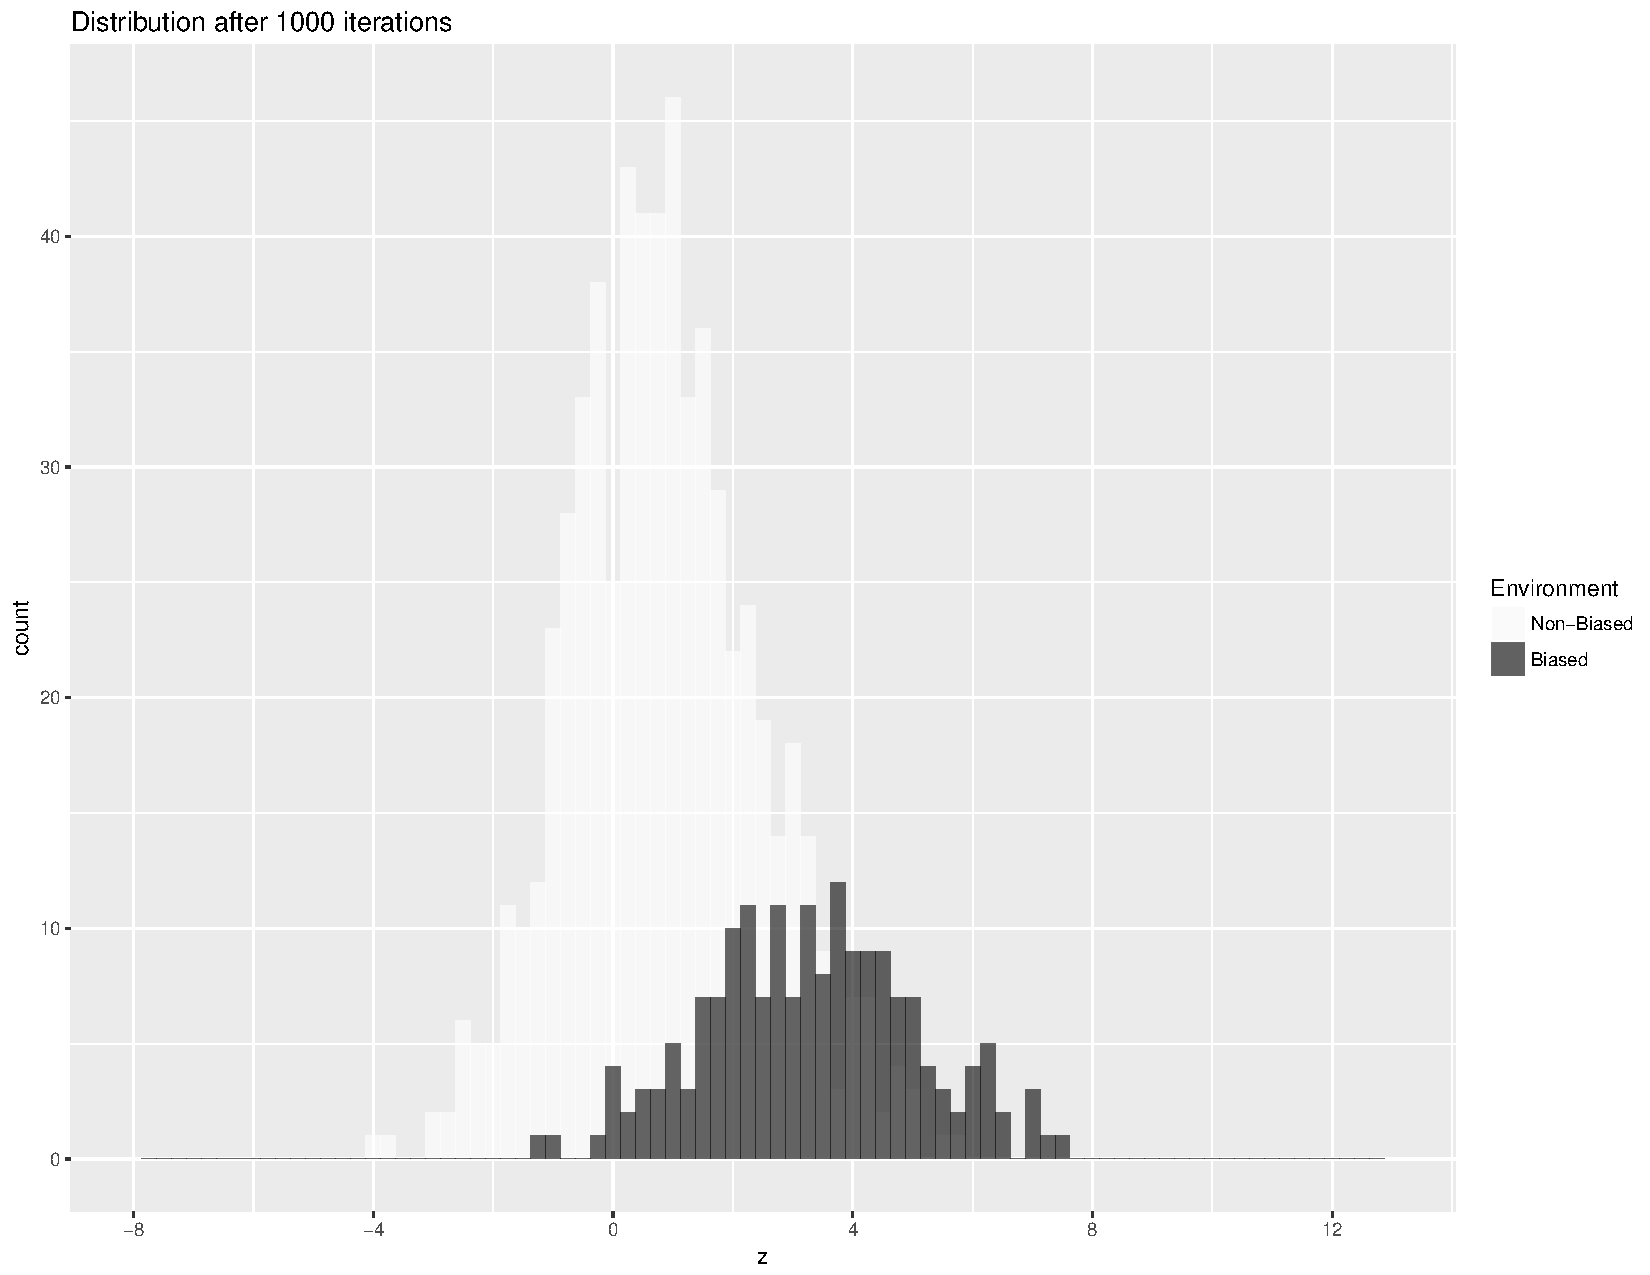
\includegraphics[width=\linewidth]{figures/1000iter.pdf}
        \caption{1000 iterations}
    \end{subfigure}\hfill
    \begin{subfigure}[t]{.45\textwidth}
        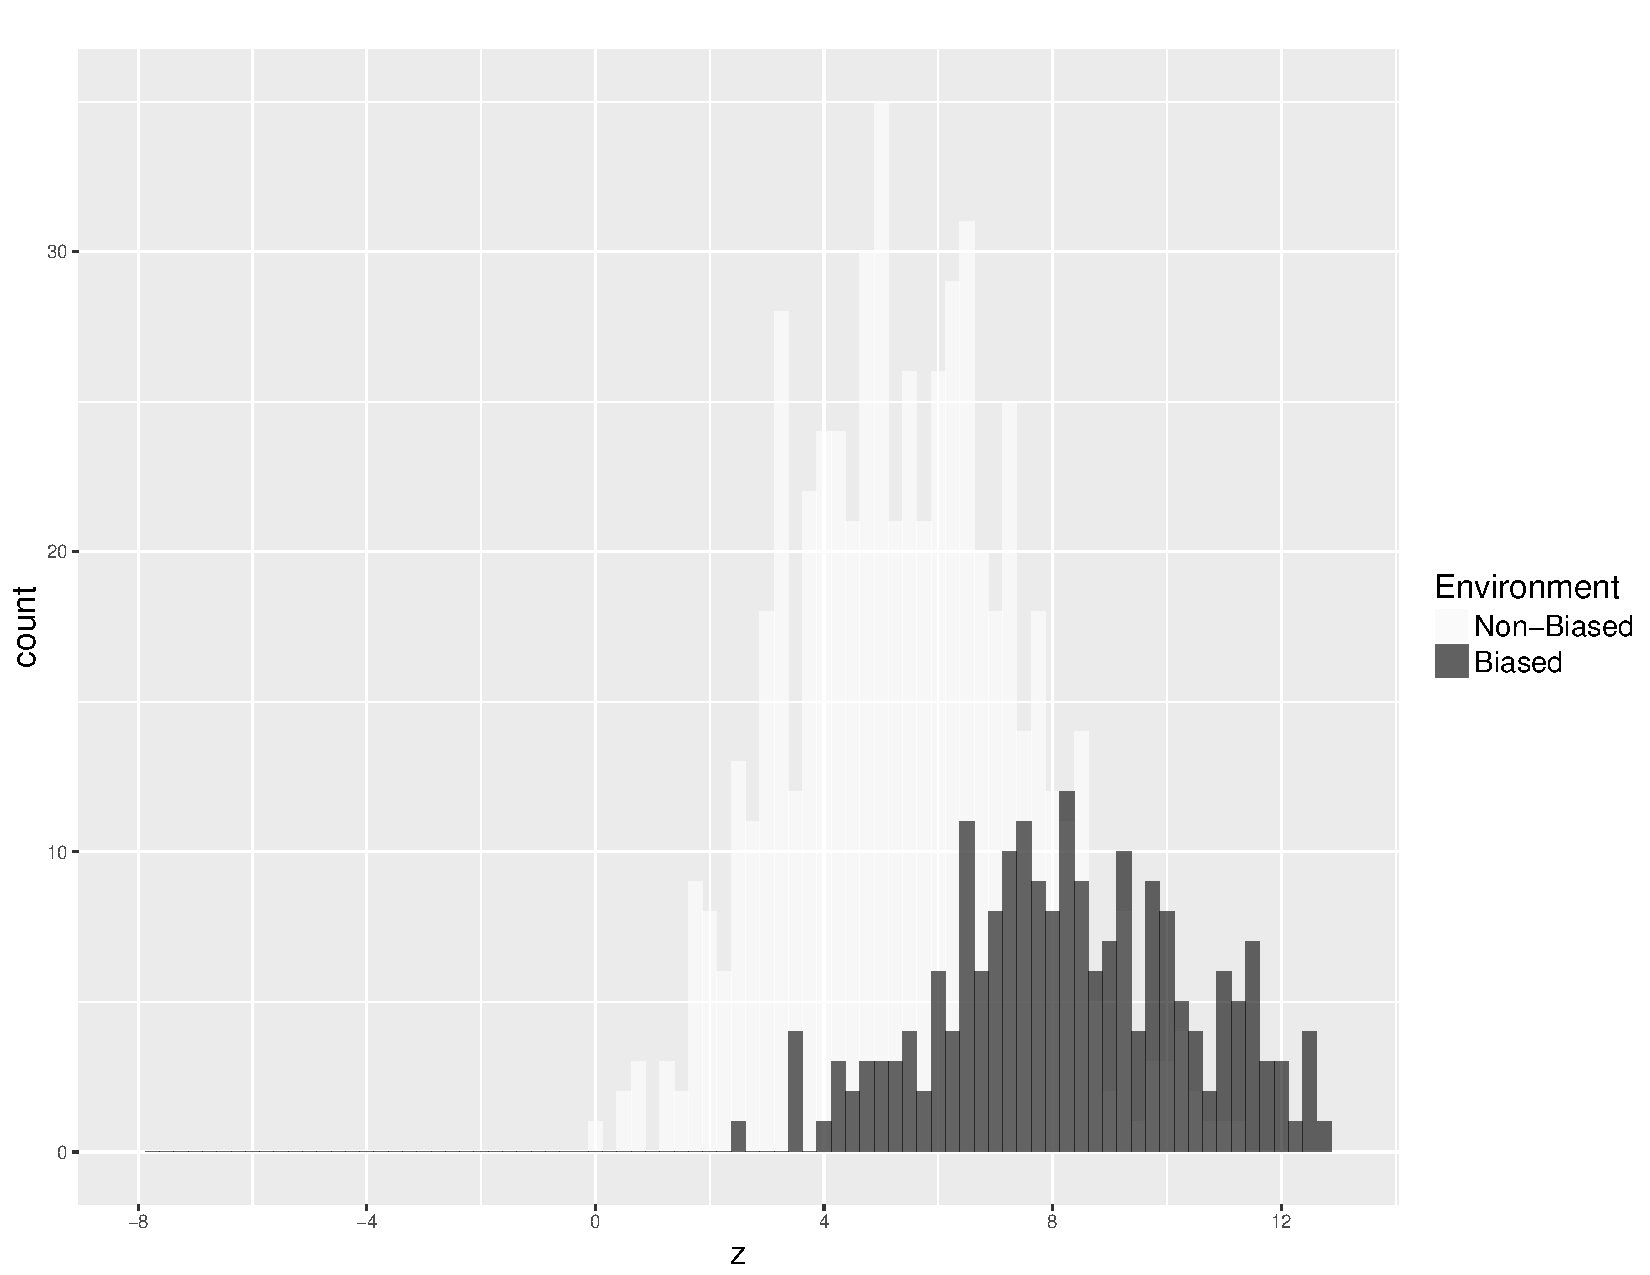
\includegraphics[width=\linewidth]{figures/5000iter.pdf}
        \caption{5000 iterations}
    \end{subfigure}
    
% % \subfloat[1000 iterations]{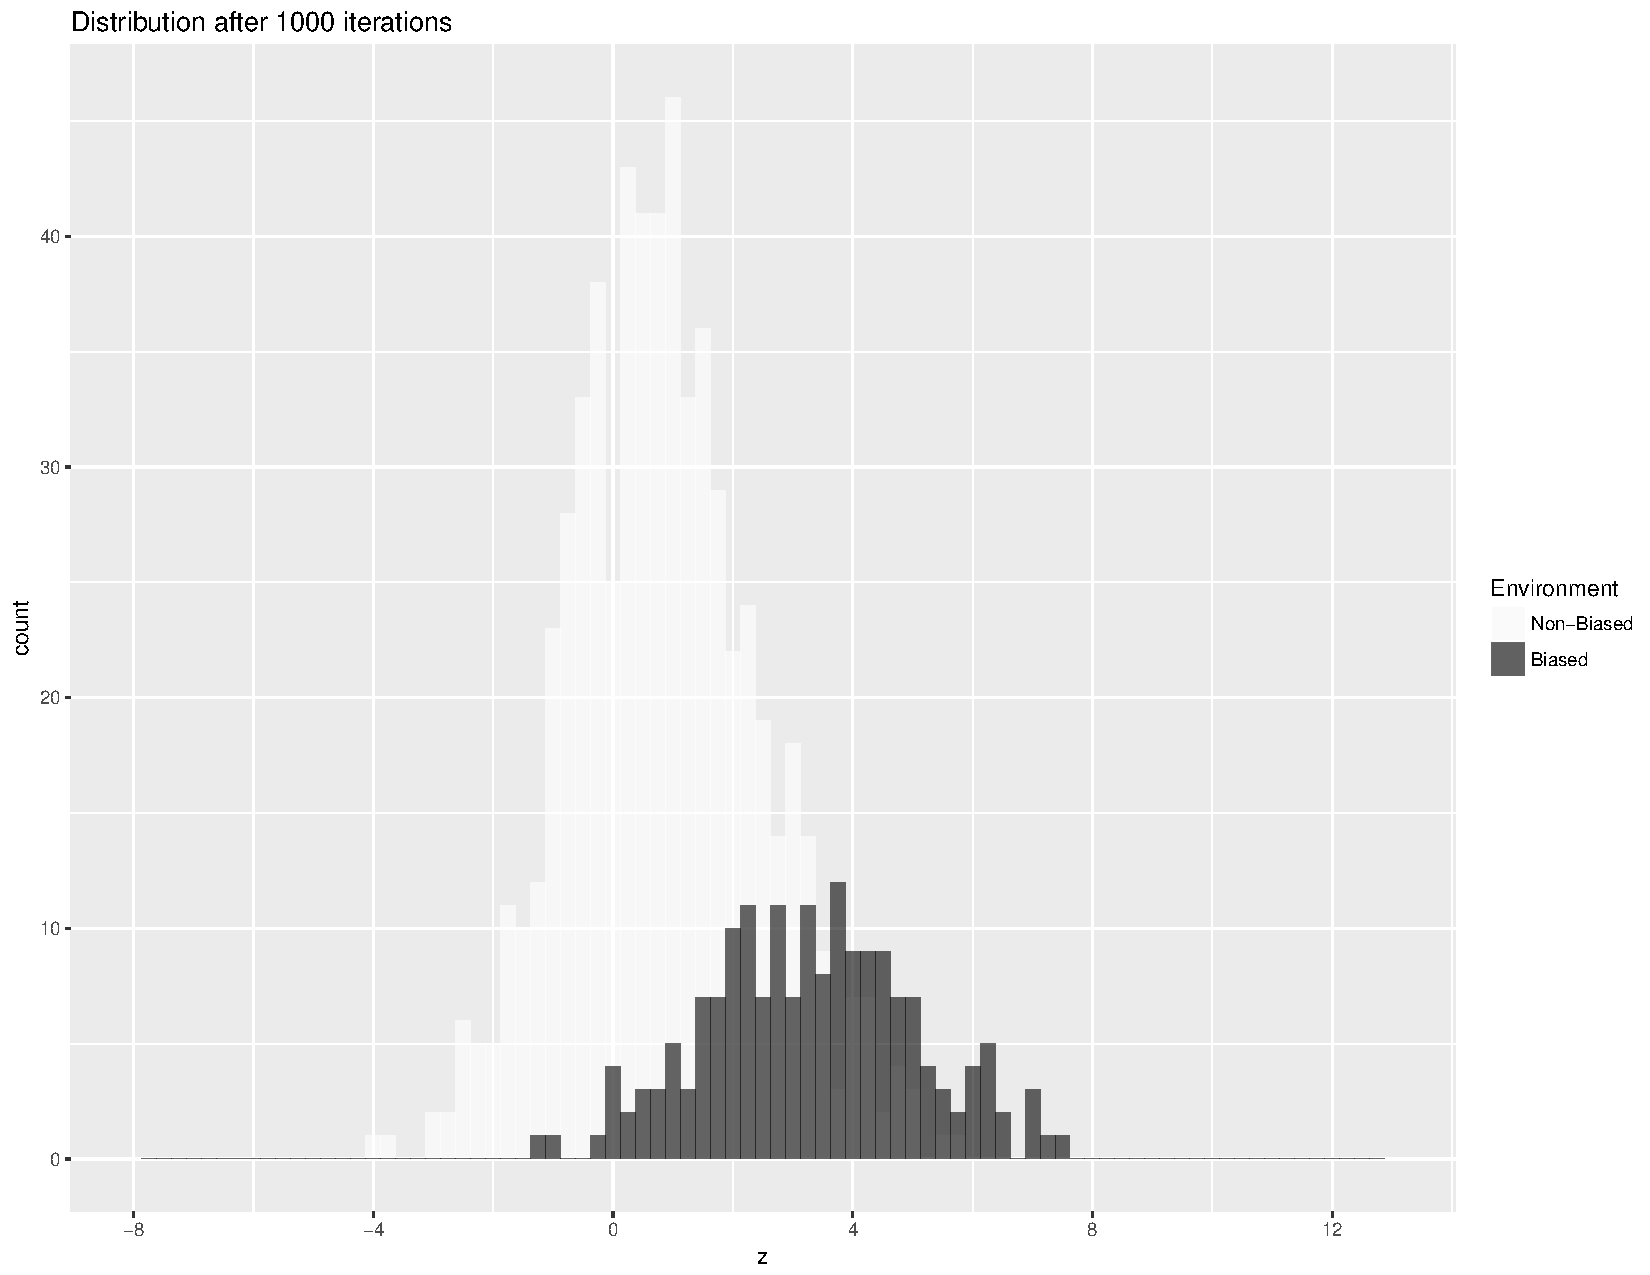
\includegraphics[width=0.3\textwidth]{figures/1000iter.pdf}}\hfill{}\subfloat[5000 iterations]{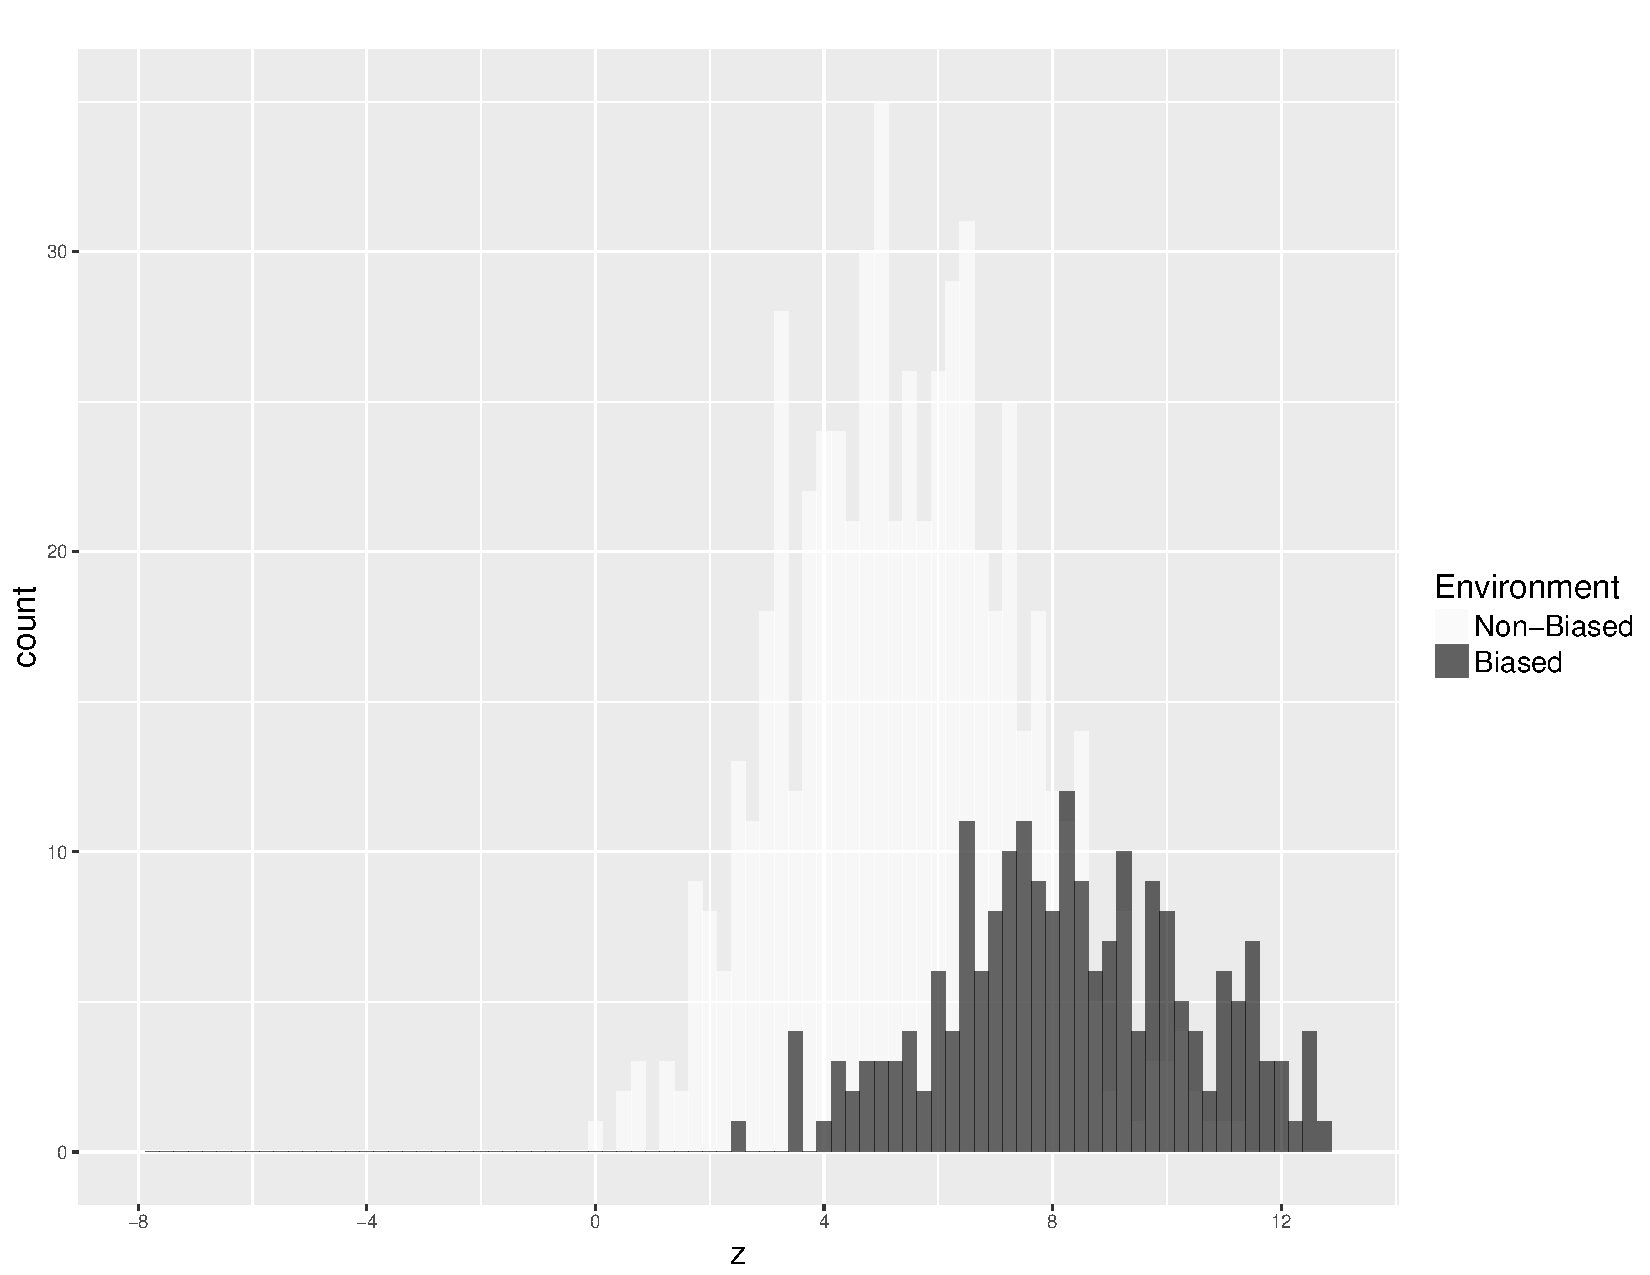
\includegraphics[width=0.3\textwidth]{figures/5000iter.pdf}}

\caption{\label{fig:End context mismatch}Observed distribution (800 tokens).
White: productions in non-biasing context. Black: productions in biasing
context.}
\end{figure}

As expected, the same unboundedness problem arises as was seen in
Model 1. With the addition of a threshold (ceiling or floor value
along \emph{x}) the sub-distributions merge, neutralizing the difference
between biased and non-biased contexts.\footnote{\citet{DBLP:journals/corr/Tupper14a} attributes a merged outcome
such as this to perfect categorization accuracy, i.e., failure to
discard ambiguous tokens. } It will also be shown that keeping all tokens in the same category,
regardless of history, results in another type of problem – what I
will call \isi{context mismatch}. Context mismatch will be discussed when
this model is linked to the linguistic phenomenon of vowel \isi{lengthening}
in Section \ref{subsec:Model-2:-Lengthening}.

\subsubsection{\label{subsec:Model-3:-Categorical}Model 3: Categorical context-dependent bias}

Model 3 implements a binary \isi{production} \isi{bias}, albeit with an error
term that maintains a small amount of variance. All tokens produced
in the biasing context are initialized with a mean at the {[}+{]} value
on dimension \emph{x}, while all tokens produced in the non-biasing
context are initialized at the {[}\textminus{]} value. See \figref{fig:binary-Starting-Distribution}.
As before, all tokens belong to the same category; the different colors
are for illustrative purposes only, allowing us to track the \isi{production}
context during the observation cycle. Because the \isi{bias} is uni-directional,
and biasing is categorical, all tokens quickly shift to the biased
{[}+{]} value. Once a token has a value of /+/ it cannot be biased
further, nor can it be ``un-biased''. This is shown in \figref{fig:binary-1000iter},
where we can see that previously biased tokens remain at {[}+{]} even
if they are subsequently produced in a non-biasing context (white
bars at {[}+{]} location). This model is, in fact, bounded, because
there is no \isi{iterativity} for the binary feature. However, like the
previous two models, it results in neutralization of the difference
between the different contexts. Binary-valued features that distinguish
between contrastive sound units within a language are widely used
in \isi{phonological} theory. This connection will be discussed when the
model is linked to the linguistic phenomenon of \isi{vowel nasalization}
in \sectref{subsec:Model-3:-Nasalization}.

\begin{figure}[H]

\begin{subfigure}[t]{.45\textwidth}
        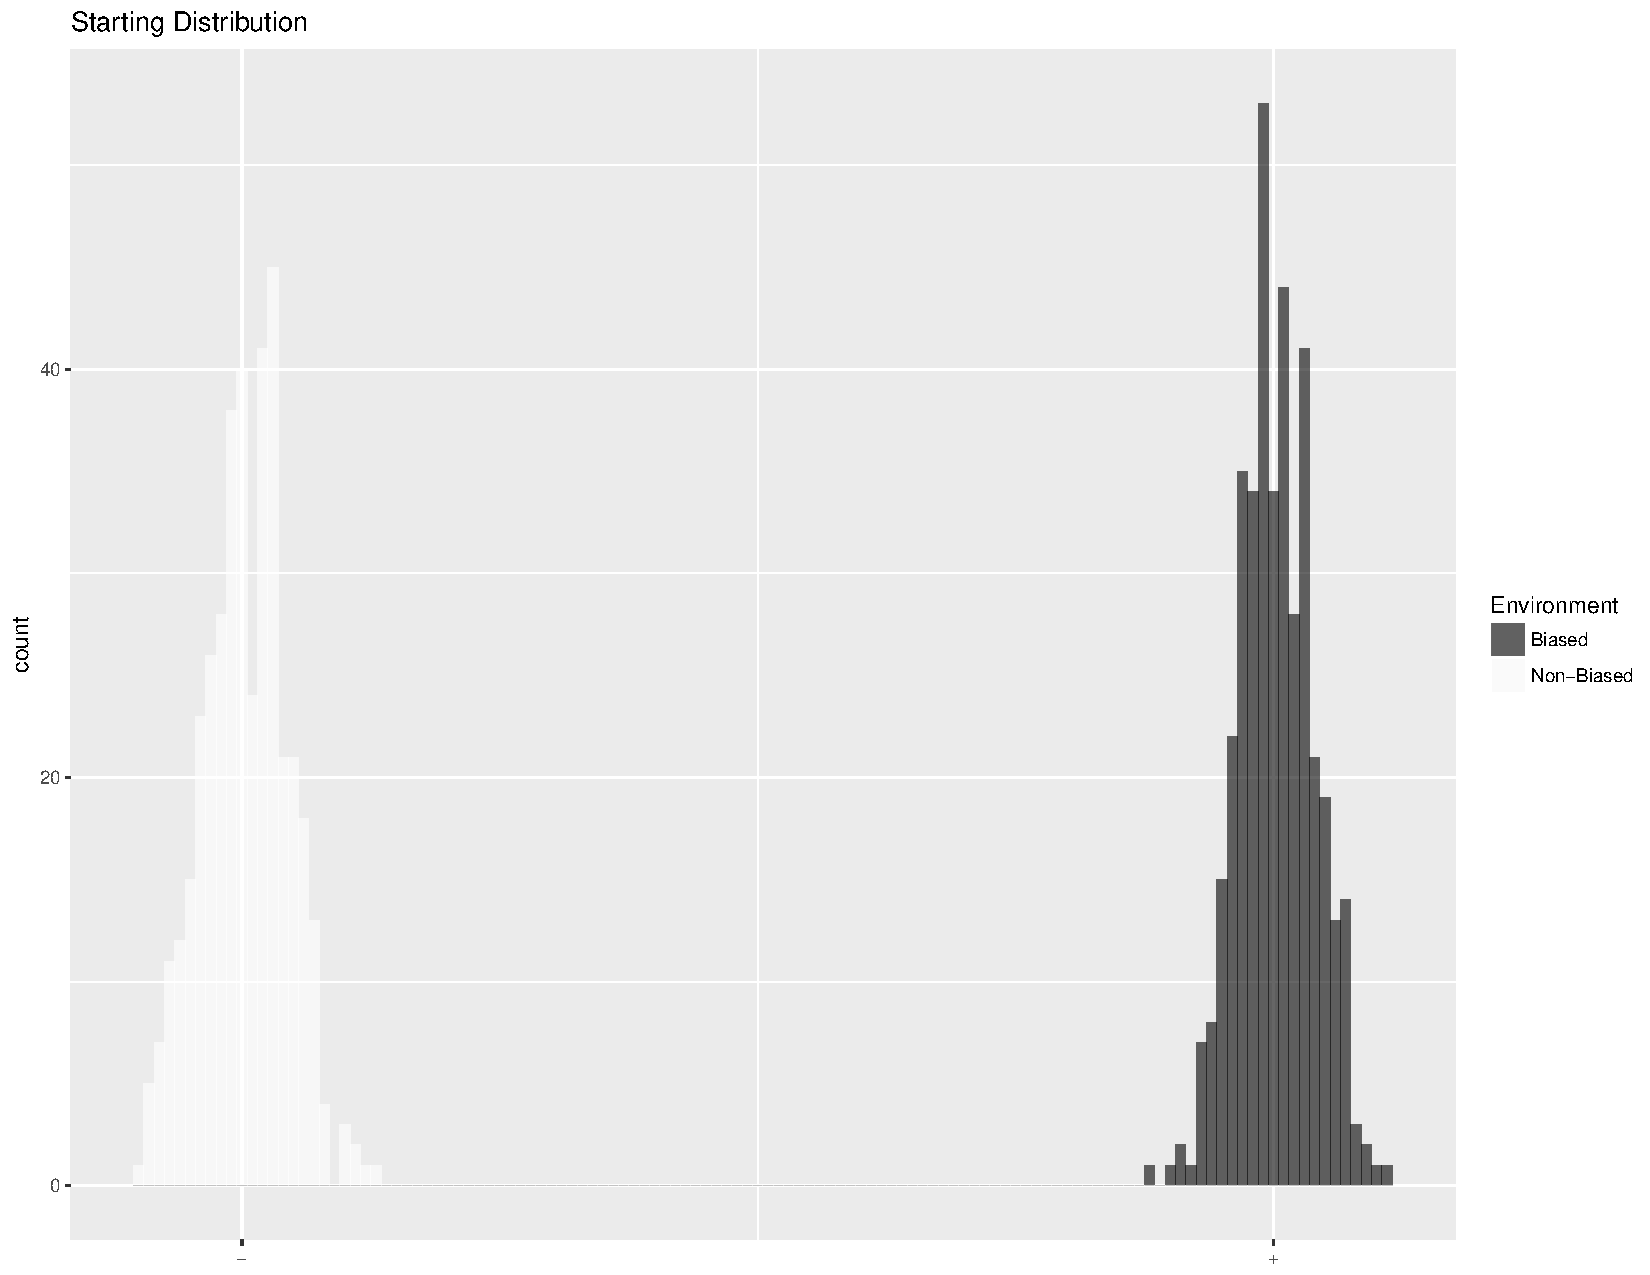
\includegraphics[width=\linewidth]{figures/NasalizationStart.pdf}
        \caption{\label{fig:binary-Starting-Distribution}Starting Distribution}
    \end{subfigure}\hfill
    \begin{subfigure}[t]{.45\textwidth}
        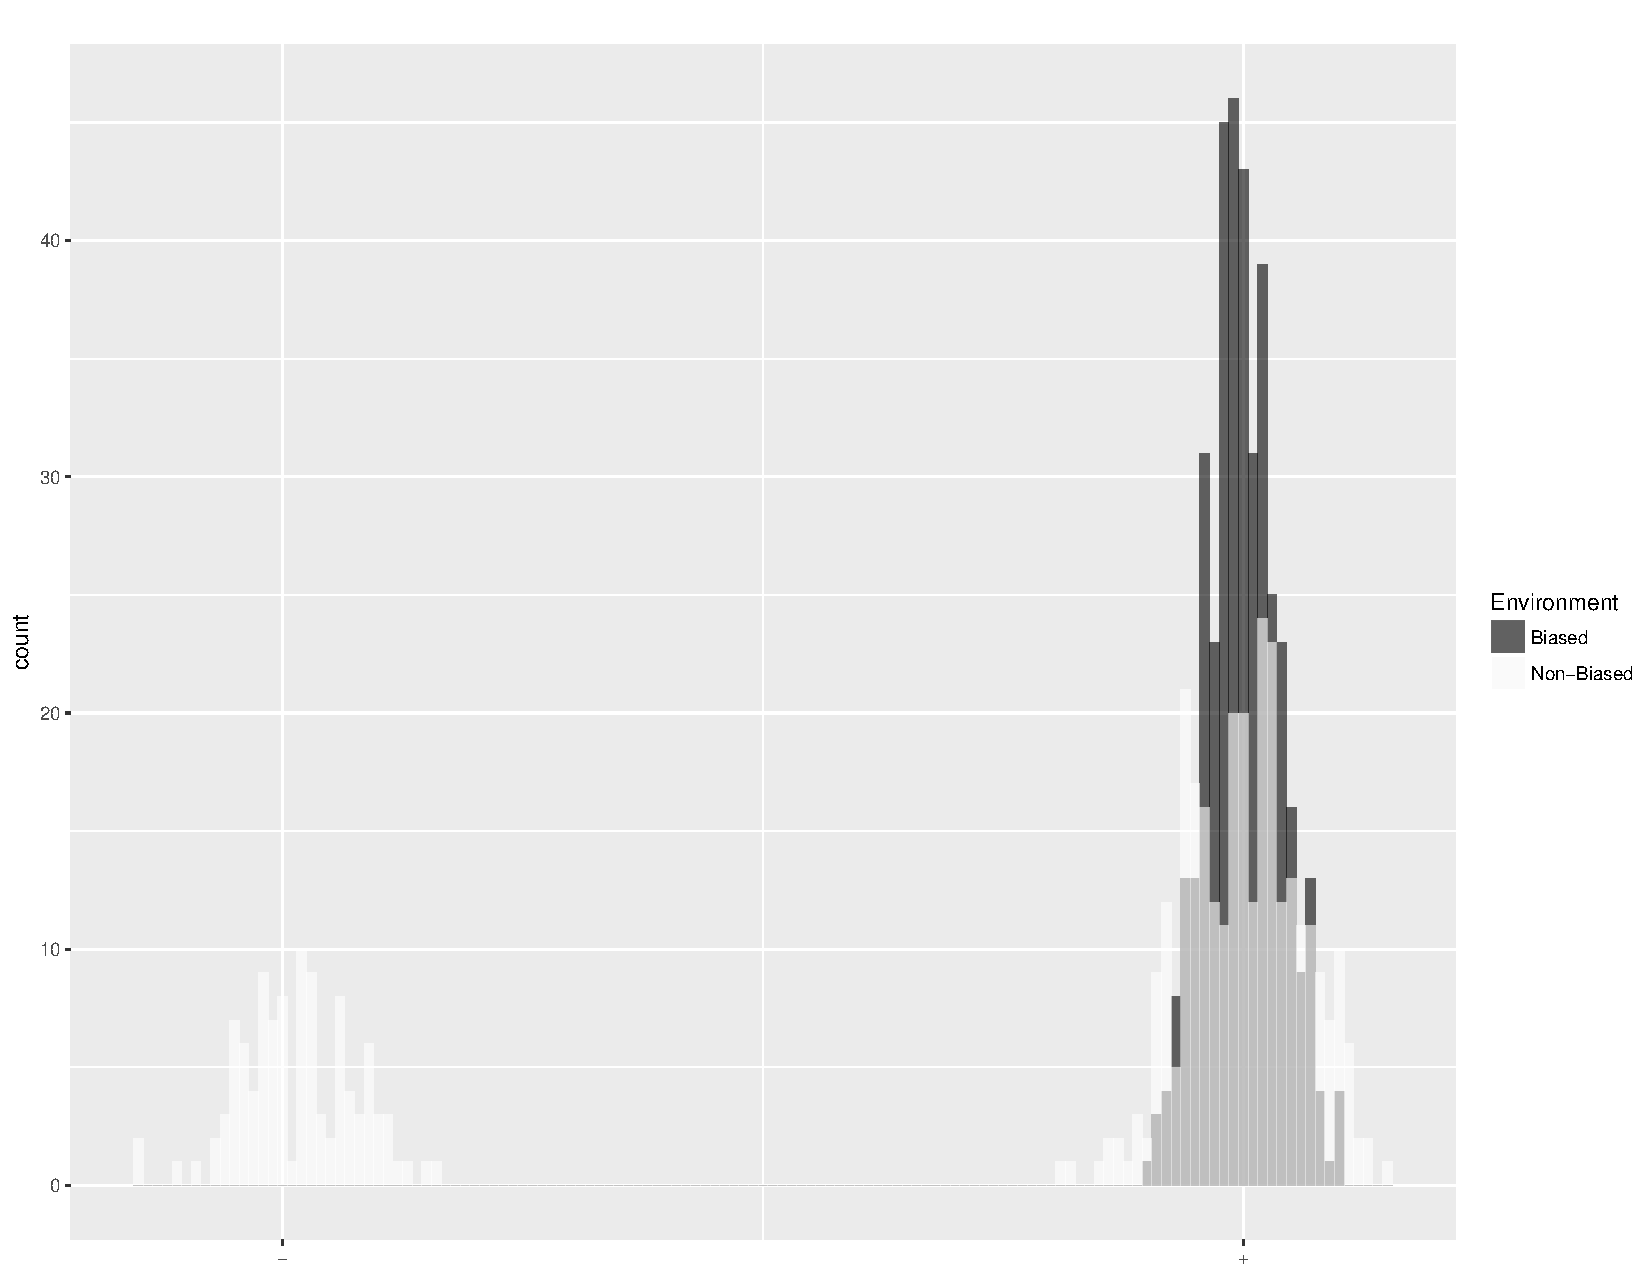
\includegraphics[width=\linewidth]{figures/Nasalization1000iter.pdf}
        \caption{\label{fig:binary-1000iter}1000 iterations}
    \end{subfigure}
% 
% \subfloat[\label{fig:binary-Starting-Distribution}Starting Distribution]{
% 
% 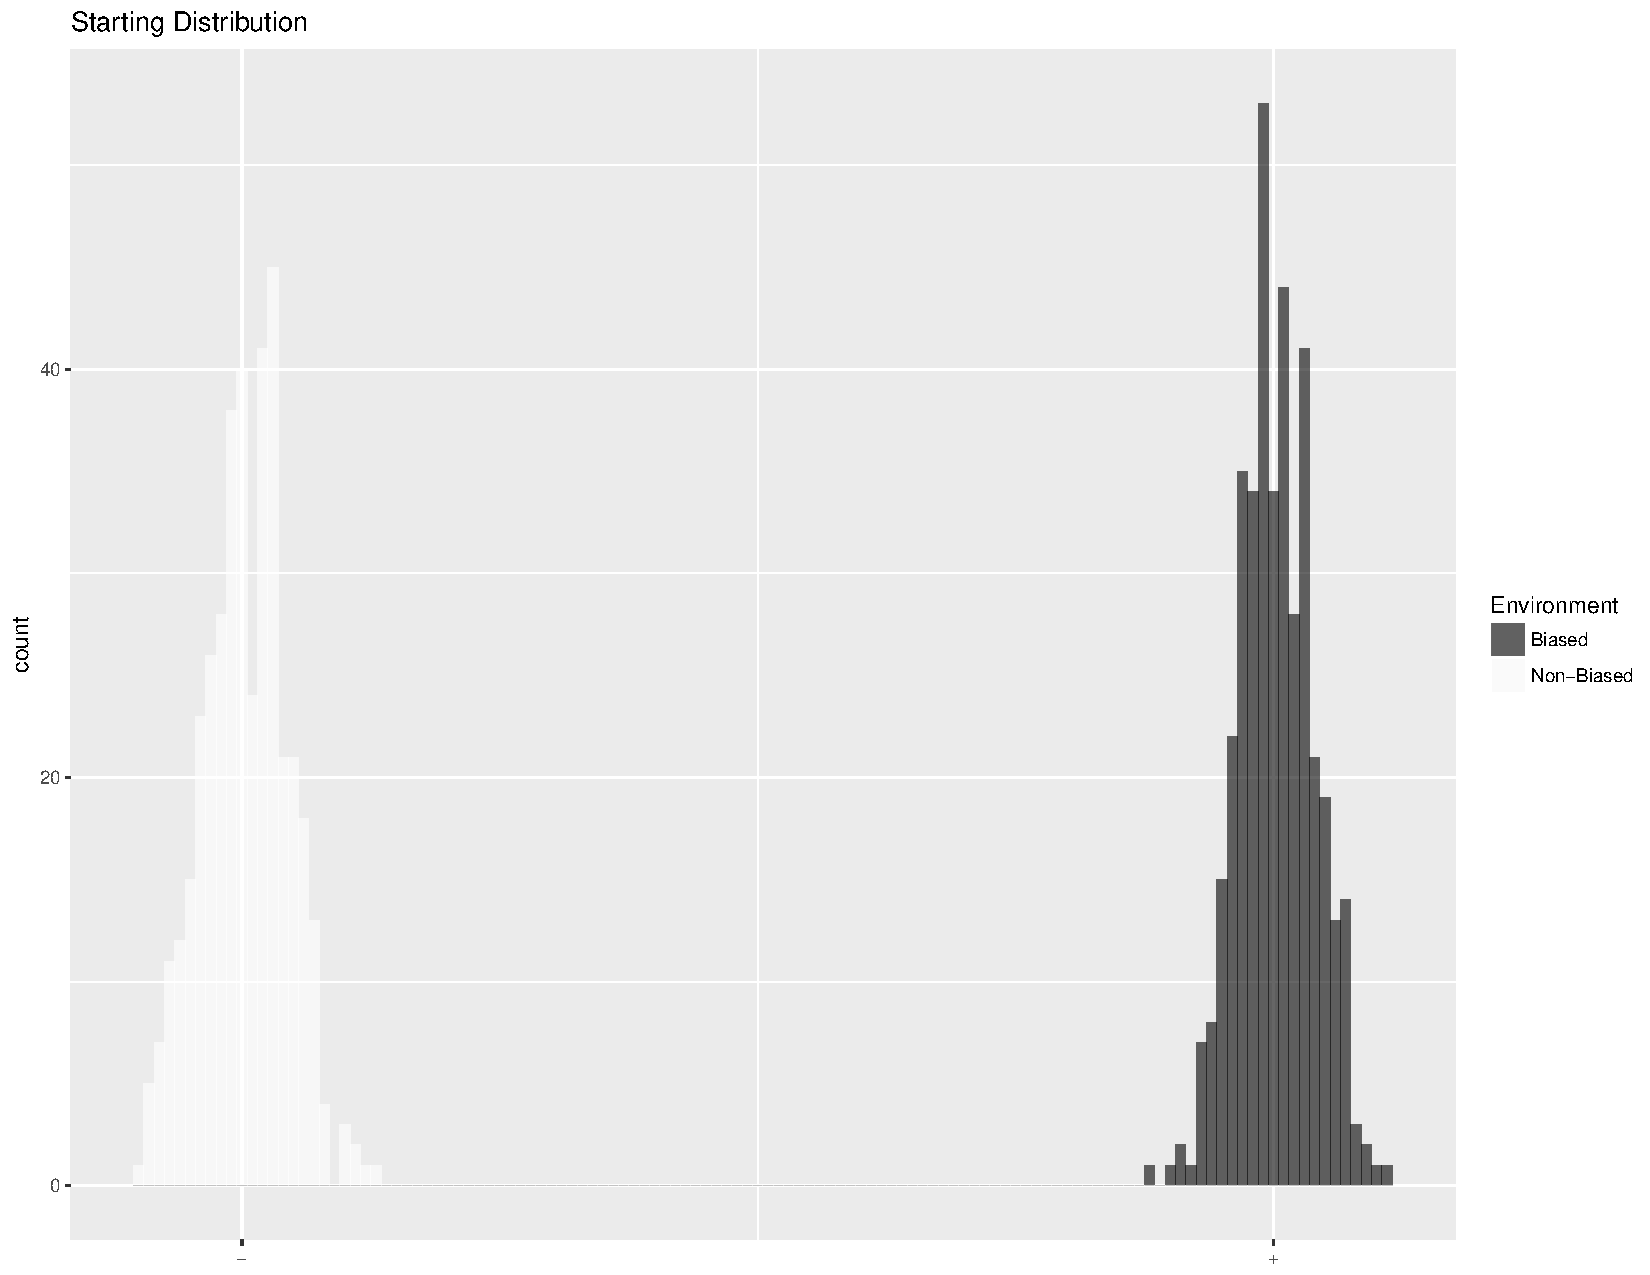
\includegraphics[width=0.3\textwidth]{figures/NasalizationStart.pdf}}\hfill{}\subfloat[\label{fig:binary-1000iter}1000 iterations]{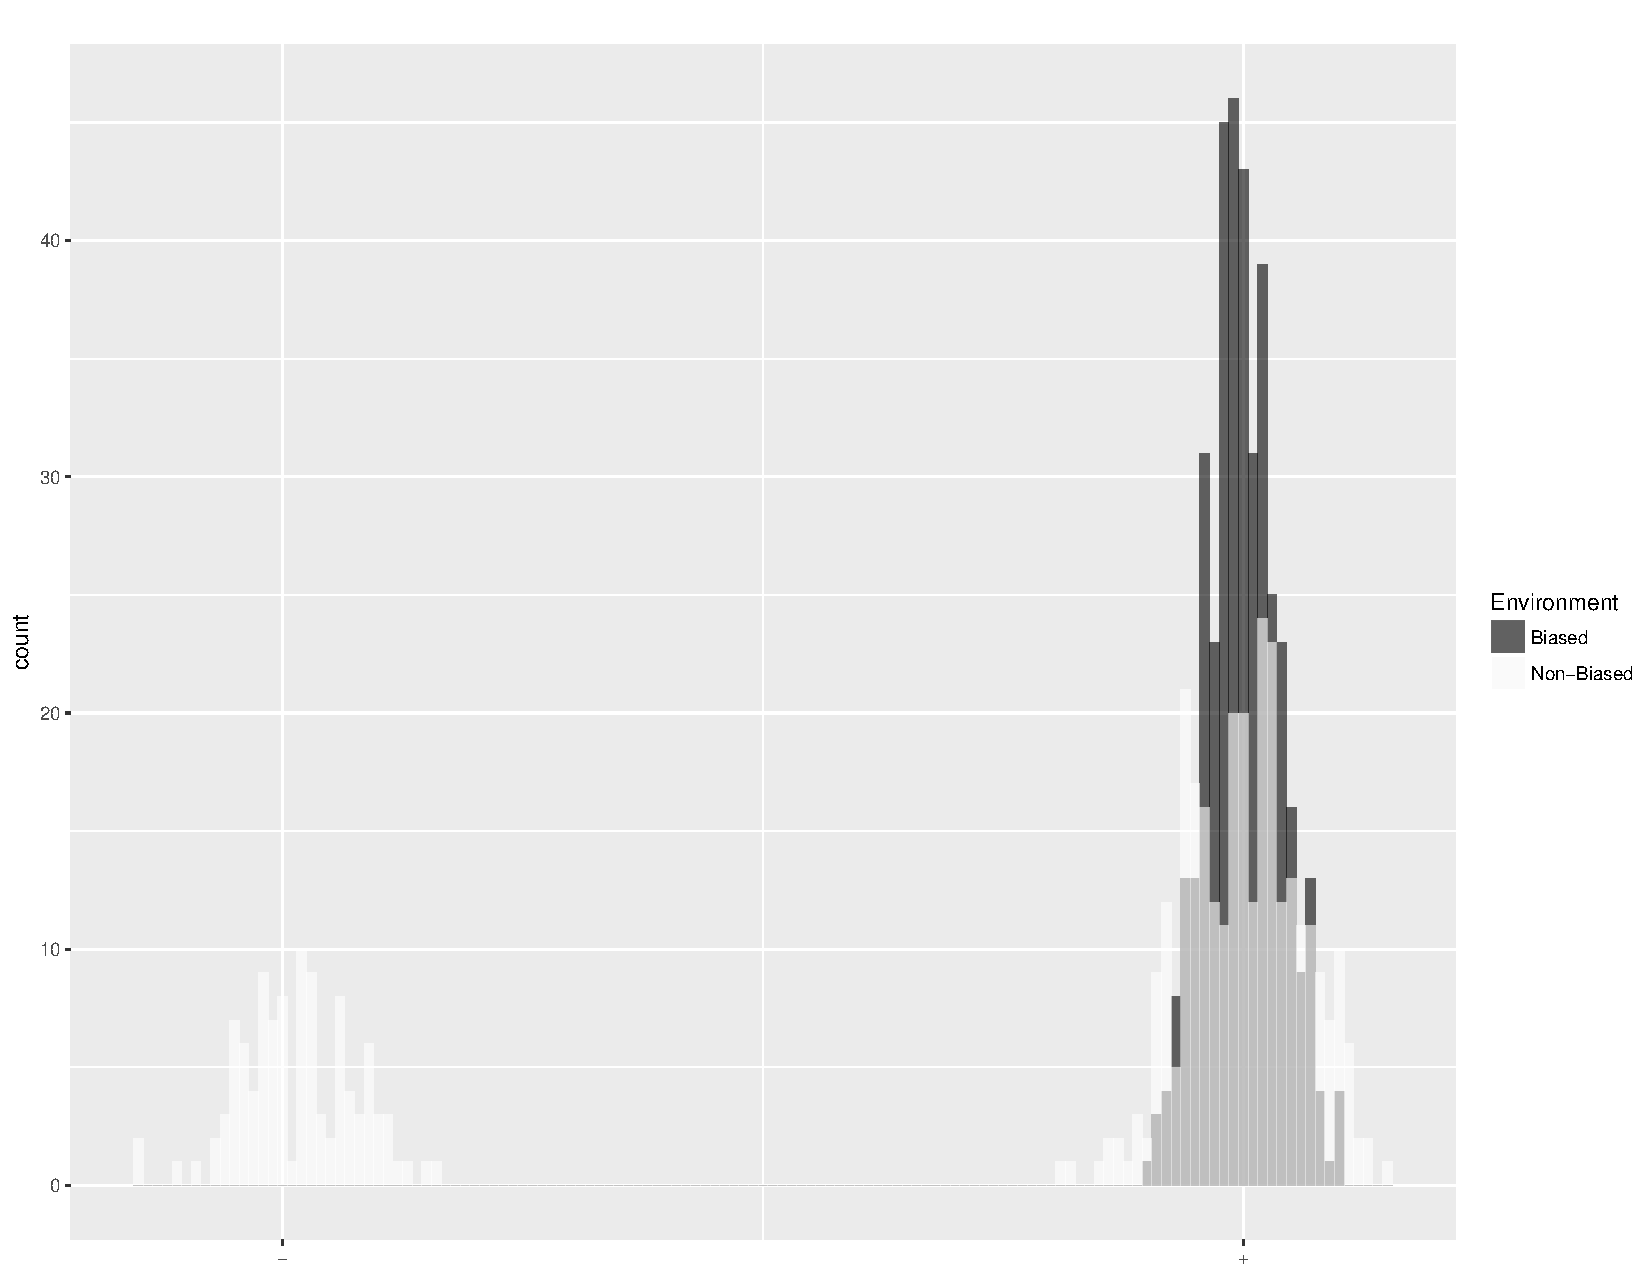
\includegraphics[width=0.3\textwidth]{figures/Nasalization1000iter.pdf}}

\caption{\label{fig:Context Mismatch Features}Quasi-binary feature. Two variants
with equal contextual frequency.}
\end{figure}

\chapter{\label{subsec:The-Linguistic-Phenomena}The Linguistic Phenomena}

The general context-free and context-dependent processes modeled in
the previous chapter will now be mapped to specific linguistic phenomena.
This chapter will show more concretely what the implementational and
conceptual issues are in developing exemplar models based on tokens
of experienced speech. We will also begin to examine the proper interpretation
of model results with respect to existing theories and, conversely,
the proper implementation of specific theoretical hypotheses within
an exemplar framework. 

\section{\label{subsec:Word-Frequency}Model 1: Word Frequency}

In laboratory speech, as well as spoken corpora, it has been repeatedly
demonstrated that words that are more commonly used are shorter in
duration than comparable words that are less common (e.g., \citealt{Bybee2001,Bybee2002,Bybee2006}).
Furthermore, it has been shown that as frequency increases, the average
duration of a given word monotonically decreases (controlling for
other factors). The diachronic counterpart of this phenomenon is the
observation that more frequent words tend to “lead sound change”,
meaning that a change that will later spread throughout all, or most,
words of a language is first observed to take place in high-frequency
words (e.g., \citealt{Phillips1984}). Such changes are often themselves
reductive in nature, either being the direct result of, or influenced
by, a reduction in the temporal, and/or spatial, extent of the articulation
of the given sounds (such as segment shortening, segment loss, assimilatory
feature changes, or feature centralization).

Competing explanations for frequency-based reduction can be separated
into listener-based and speaker-based approaches. In the former, more
reduced forms are assumed to be easier/more efficient for speakers
to produce, and are thus hypothesized to be the default production
mode. However, in the case where the meaning is unclear, or there
is greater than normal ambiguity, the speaker exerts more effort in
articulation, lengthening and strengthening speech sounds in order
to facilitate speech recognition for the listener (e.g., \citealp{Aylett2004}).
Because words that are highly predictable in context are easier to
recover, such words can be safely reduced, whereas less predictable
words must be produced more carefully. In the absence of other factors,
the marginal probability of a given word provides an estimate of its
likelihood; thus low-frequency words will be produced with less reduction
in order to facilitate their recovery relative to high-frequency words.
A speaker-based approach, on the other hand, attributes frequency
effects to automatic consequences of speech production. Either high-frequency
words have higher resting activation levels on average, leading to
faster retrieval, and thus more rapid articulation (e.g., \citeauthor{gahl2012reduce}),
or increased practice with higher-frequency words leads to greater
fluency, resulting in shorter, more efficient articulation (e.g.,
\citealt{Bybee2002}).

\citet{Pierrehumbert2000} adopts a speaker-based motivation for reduction,
modeling the effect as a production bias that shortens each token
by the same small fixed amount whenever it is produced. Although a
model containing both high and low frequency categories was not actually
implemented in \citet{Pierrehumbert2000}, the paper suggests that
this simple bias can account both for synchronic differences in word
duration, as well as reductive changes, over time. 

The more often tokens are produced from a given category, the more
chances there will be for initially unreduced tokens to be reduced
multiple times. Thus, it might seem to follow that higher-frequency
categories will shift further leftward than lower-frequency categories
over the same period of time. However, as we saw in Section \ref{subsec:Model-1:-Context-Free},
the relative average durations of a lower- and higher- frequency word
category depend on whether the number of tokens in a given category
is proportional to the frequency of that category. Furthermore, given
enough time (= number of productions), all categories will end up
at the same minimum duration. In other words, the model will converge
on this one stable state from any starting point. This is the inevitable
result of a model with an unopposed force acting, and thus is not
particularly surprising (\citet{Baker2011} make a similar observation
about gradual-accumulation theories of change in general). However,
it raises an important issue regarding the determination of synchronic
versus diachronic time in exemplar models. 

Computational models are typically only evaluated at convergence.
This is in part because there is usually no explicit theory about
how time within a model corresponds to real time (or to time in some
other model). Exemplar models, however, explicitly map iterations
to real-world events, namely, the perception and storage of speech
tokens. This requires that literally any stage of the model be a possible
synchronic state – at least an instantaneous one. This property also
makes it possible, in principle, that the state of the model at convergence
(or the fact that the model fails to converge) is irrelevant to evaluation.
This is the case if it can be shown that convergence does not occur
within the lifetime of the speaker. If the model parameters are chosen
in a specific way, collapse may be avoidable within whatever is taken
to be an average lifetime. An illustration of what is required to
determine these parameters is provided in Appendix \ref{chap:Appendix B}.
This line of enquiry uncovers a further prediction of this general
model. It must be the case that all words become more reduced over
time, regardless of the specific parameter values. 

The iterative model strongly implies that the frequency effect must
arise in the lifetime of the speaker, and only after they have had
sufficient exposure to a given (high frequency) category. We will
define this timespan as the time it takes a category of some frequency
\emph{f,} with a reduction bias of $\alpha$, to reach a degree of
reduction, $\delta_{n_{f}}$, that is expressed as a proportion of
the original duration. We will call this amount of real time an epoch,
and we will define the number of productions of category \emph{f}
during an epoch as $n_{f}$. Then, by definition: $\overline{d_{n_{f}}}=\overline{d_{0}}-\delta_{n_{f}}\overline{d_{0}}$.
Since we know that a frequency effect is observable, at minimum, in
young adults, this epoch cannot be longer than around 20 years. Unless
\emph{f }decreases drastically (in fact, we might expect it to increase
at this life stage), then multiple epochs remain in the lives of these
speakers, and a decrease comparable to the original frequency effect
should be expected to occur in each one of them. Thus, we should find
that word durations should get steadily shorter over the lifetime.
Of course, there is a hard limit on how much a word can be reduced.
If we predict that some words will hit this limit within the given
time frame then the frequency effect should actually be lost in the
subset of words that have reached this limit. Although I am not aware
of any studies that have specifically investigated these questions,
I strongly suspect that these predictions would not be borne out.

\section{\label{subsec:Model-2:-Lengthening}Model 2: Vowel Lengthening}

Context-dependence is the norm in language, especially in the domain
of sound structure. Speech sounds exist in a high-dimensional space,
and almost any change in context produces some measurable difference
in a sound's pronunciation along one of those dimensions. These effects,
however, are usually predictable, and so can be modeled using a fixed
bias. Vowel lengthening before voiced obstruents in word-final position
provides a simple instantiation of a context-dependent phenomenon
that applies to the duration dimension. It has been noted for well
over a 100 years that vowels before final voiced obstruents in English
are “very long” (\citealt{Sweet1880}: p 59), and laboratory
studies have consistently found significant vowel duration differences
between voiced-voiceless minimal pairs like “bad” and “bat”
(e.g., \citealt{peterson1960duration,chen1970vowel}). Furthermore,
perceptual experiments find that vowel duration is a sufficient cue
to the “voicing” on the final obstruent, whether that segment
is actually voiced or not (e.g., \citealt{raphael1972preceding,Klatt1976}).
As it is conventionally described, vowel lengthening is an allophonic
process whereby vowels produced in the lengthening context (before
voiced obstruents) are lengthened by some degree, while vowels not
produced in the lengthening context remain unchanged.

However, the results of the Model 2 simulation show that, over time,
“short” tokens gets longer, and “long” tokens get even
longer, and eventually all tokens are maximally long whether they're
produced in pre-voiced or pre-voiceless contexts. Furthermore, it
is not possible to guarantee, at any intermediate stage, that tokens
produced in the biasing (voiced) context will be consistently longer
than tokens produced in the non-biasing (voiceless) context. Because
of the different possible histories of each token, the single category
contains both tokens that are very long (all ancestors produced in
biasing context), and very short (all ancestors produced in non-biasing
contexts). If a particularly short token is chosen (at random) for
production in a voiced context it won't be as long, even after lengthening,
as other tokens in that context have been in the past (on previous
iterations). Likewise, if a particularly long token is chosen to be
produced in a voiceless context it will be longer than other tokens
in that context have tended to be. We know that listeners develop
expectations about what they should be hearing based on context, and
can detect when the variant differs from expectation (e.g., \citealp{krakow1988coarticulatory,gaskell1996phonological}).
This mismatch between token and context is therefore a problem for
the basic exemplar model. 

However, all these effects can be seen to arise out of the fact that
all tokens are taken from, and added back to, the same undifferentiated
cloud. If tokens of the two allophones were stored separately, then
these problems could presumably be eliminated. Let us consider what
that would entail. From the perspective of theoretical linguistics,
allophones, by definition, have no independent representational status.
They exist only at the surface, only as the realization of a phoneme
to which some rule, or process, has applied\footnote{Note that this model is entirely implemented at the phoneme level,
allowing the presumed forces to act directly on their targets. Although
exemplar models often assume a word-level representation (explicitly
or implicitly), most are actually implemented at the phoneme level,
and lack explicit mechanisms for connecting the two (although see
\citet{Wedel2008} for a model of an indirect biasing relationship).
Mechanisms such as frequency-based reduction and contrast maintenance
are defined with respect to the word level. Implementing them at the
sub-lexical level not only obscures the fact that a mapping between
the levels is necessary, but eliminates a fundamental property of
abstraction: the more abstract the unit, the larger the category,
and the more, and more varied, the tokens. The phoneme category \textipa{/æ/}
encompasses more than just tokens extracted from the words “tag”
and “tack”, but from a large number of words, such as “cat”,
“lack”, “sag”, “package”, etc. Any changes at the
level of the individual word are only one small part of what affects
the realization of a given phoneme. Thus, establishing that a phoneme-level
effect follows from a word-level interaction requires a significantly
more complex model than is usually implemented. }. We are perfectly free to adopt the hypothesis that allophones do,
in fact, have separate representational status, and create a model
in which “lengthened” allophones are only selected from the
“lengthened” (sub) category, and only “unlengthened” allophones
from the “unlengthened” (sub) category\footnote{This is implemented as the State Model in Chapter \ref{sec:Models-of-Change}}.
This would eliminate the context-mismatch problem. A paradox arises,
however, if we continue to apply the lengthening bias to the lengthened
tokens. By creating a category for these allophones we are effectively
encoding their context: this category consists of tokens that occur
before voiced obstruents. Applying lengthening to such a token implies
that the token was original unlengthened (non-biased). It also implies
that the contextual information was discarded when the token was stored,
and so must be added during production. A model with both explicit
representational structure incorporating a biasing context, and an
actual biasing process, is a strange hybrid. This incompatibility
between modeling a phenomenon as both stored \emph{and} generated
will be discussed in more depth in Chapter \ref{sec:Models-of-Change}. 

\section{\label{subsec:Model-3:-Nasalization}Model 3: Vowel Nasalization}

While phonemes are taken to be the basic phonological unit for many
purposes, most phonological rules that operate at the level of individual
phonemes, in fact, affect only a subset of that phoneme's features.
Classically, phonemes are taken to be decomposable into a universal
set of discrete features, and can be uniquely defined by a specific
matrix of values over those features. These features are usually assumed
not just to be discrete, but to be binary in nature, taking on only
one of two possible values, “+” or “-”. Thus a partial
feature matrix might consist of $\left[\begin{array}{c}
+voice\\
-nasal\\
+coronal\\
-del.rel
\end{array}\right]$, for example, which matches the phonemes /\emph{t}/, /\emph{d}/\emph{
}and /\emph{s}/, among others. Whether considered to be phonetic or
phonological, nasalization is a process that changes the $\left[-nasal\right]$
specification to $\left[+nasal\right]$. In English this rule applies
to all vowels occurring in the context of a following nasal consonant
(e.g., \textipa{[læb]} vs. \textipa{[læ̃m]}). Thus it is analogous,
in all respects other than binarity, to the vowel lengthening example
simulated in Model 2, and similarly results in context mismatch. What
Model 3 demonstrates more transparently, however, is that the eventual
outcome is neutralization of the distinction between the two allophones.
Once a given token is produced in a nasal context for the first time,
all its daughter tokens will also be nasal, even when produced in
an oral context (\textipa{[læ̃b]}). Neutralization occurs because
the process of nasalization is uni-directional; nasalized tokens produced
in oral contexts are not `oralized'. In other words, there is only
one bias, and only one biasing context, and under those circumstances
the basic exemplar model will result in biased variants in all contexts.

The nasalization rule, in addition to illustrating a binary process,
introduces a biasing dimension other then duration. This is important
because duration is significantly simpler than most phonetic variables.
Additionally, duration possesses what may be a unique property: it
is invariant under the transformation from production to perception
(in the absence of error)\footnote{There is, however, potential ambiguity in attributing duration differences
to inherent duration, versus differences in speaking rate or prosodic
contexts. See Chapter \ref{subsec:Summary-=000026-Conclusions}. }. Thus, an architecture that can derive the correct results for phonological
processes acting on duration is not guaranteed to do the same for
other phonological dimensions. 

Vowel nasalization seems to be quite well-understood, and to have
a straightforward explanation. It arises through an inherent property
of normally produced speech: coarticulation. The articulation for
the nasal consonant, which involves lowering the velum so that air
can flow through the nasal cavity, is initiated before the articulation
of the preceding vowel is fully completed. As a result, the velum
is open for some portion of the end of the vowel, meaning that nasal
airflow occurs, which, by definition, means that the vowel is partially
nasalized. The evolution from partial to full nasalization seems to
be exactly what the basic exemplar model should account for: a gradual
increase of nasalization through an iterative process in which already
nasalized (biased) tokens are subject to additional nasalization (biasing)
as produced tokens are converted into stored tokens, which are once
again converted into production tokens. Yet we have already seen that
the context-dependent version of the basic exemplar model results
in a single degenerate outcome. 

In fact, there is a deeper representational problem related to the
source of the bias. The degree of vowel nasalization corresponds more
or less directly to the extent of the vowel during which nasal airflow
is present. Thus, it is a question only of how early the velum is
lowered. For nasalization to increase incrementally, the velum lowering
must occur earlier and earlier. There is, however, no mechanism in
the basic exemplar model to accomplish this. The root of the problem
is the lack of an explicit production to perception mapping. That
mapping will be the focus of Chapter \ref{sec:Perception-Production}.
For now the focus will be on the production side, and the argument
will be that, on empirical grounds, articulatory parameters cannot
depend solely on the free evolution of perceptual categories. Chapter
\ref{sec:Models-of-Change} will also show that explicit articulatory
targets can be used to prevent the collapse and merger problem shared
by Models 1-3.
\chapter{\label{sec:Models-of-Change}Modeling Stability \& Change}

In many implemented exemplar models that include production, unbounded
iterative biasing is prevented via the elimination of tokens that
fall in the ambiguous region between two existing categories (\citealp{Wedel2004,Wedel2006,Wedel2008,Blevins2009,DBLP:journals/corr/Tupper14a}).
If the categories are taken to be words, then discarding ambiguous
tokens acts to maintain a meaning distinction that relies on a minimal
sound distinction along the given phonetic dimension. The idea that
sound changes that produce homophony are dispreferred in some way
has existed within historical linguistics for a long time (e.g., \citealt{Martinet1955}).
In recent years this notion has been revived and quantified as an
inverse correlation between the probability of a sound change that
neutralizes contrast \emph{x}, and the number of words that are differentiated
only by contrast \emph{x}. This is known as the “functional load”
of the contrast\footnote{There are many other ways one might define functional load. However,
it turns out that a simple minimal pair count seems to be the most
useful of these.} (\citealp{Surendran2006,wedel2013high}). In \citet{Wedel2008},
contrast maintenance (homophone avoidance) is implemented as a storage
probability that is proportional to goodness of fit. Tokens that are
less prototypical members of both categories have a lower probability
of being retained in either category. Thus, as ambiguous tokens are
lost, the two categories are effectively pushed apart. Functional
load can be modeled as a weighting factor in this type of model, increasing
the probability that ambiguous forms will be discarded, and effectively
strengthening the contrast maintenance effect for certain words (\citealt{Soskuthy2015}).

The existence of a second contrasting category along the biasing dimension
will prevent the biased category from moving past a certain point,
allowing the basic exemplar models of the previous chapter to converge.
The assumption of such a category, however, limits the types of sound
changes that can be modeled; in particular, a sound change in which
a new category is formed, presumably from the biased variants of an
existing category. It is exactly this change that is adopted as the
modeling gold standard in this book. Therefore, we will have to consider
what other forces can achieve stability, forces that, if general,
must be included in all models, whether they are implementationally
necessary or not\footnote{A goodness-of-fit function that doesn't directly reference contrast
is possible in this scenario. However, it will not produce the desired
effect for a single category. If prototypicality is determined by
distance from the category mean, then what is acceptable will change
as the mean of the category changes, which will occur because of the
constant phonetic bias. Therefore, the category will move unboundedly.
On the other hand, if prototypicality depends on some fixed value,
then the category will not be able to shift beyond the specified limit
of `goodness'. }. In this chapter we will analyze, in detail, the consequences of
adding production targets to the basic exemplar models of Chapter
\ref{sec:The-Exemplar-Model}. In doing so we will arrive at a subset
of models that meet the two criteria of boundedness and theoretical
coherence. The full range of possible outcomes for this set of models
will then be derived, setting the stage for an investigation of what
type of architecture would be sufficient (and possibly necessary)
to produce (under the appropriate conditions) the genesis of a new
phoneme category.

It should be noted at this point that it is widely acknowledged that
sociolinguistic factors play a central role in language change. A
class of `innovators' may be required, aided by a class of `early
adopters' in the actuation and spread of a change (\citealt{milroy1985linguistic}).
Change may require those with less social power to pay more attention
to the speech of those with more power, leading to incorrect inferences
about the source of phonetic variation (e.g., \citealt{Garrett2013}).
Change may require systematic differences between individual speakers
in their analysis of ambiguous data, the degree to which they compensate
for phonetic biases, or some other facet of speech processing (e.g.,
\citealp{Beddor2009,yu2013socio}). This paper does not explicitly
address these aspects of sound change in that it focuses on the mental
grammar of a single individual. The approach taken here, however,
is not incompatible, nor inconsistent, with a theory of sound change
that includes socio-indexical variables.

\section{Articulatory Targets}

Many of the set of proposed universal phonological features specify
articulatory parameters, such as where in the mouth the tongue tip
makes contact during the production of the sound. Explicit targets
of this kind are often assumed to be unnecessary in exemplar modeling,
where categories are taken to be emergent – dependent only the interaction
of competing forces. This assumption is aided by the practice of treating
the initial distribution of tokens as arbitrary and independent of
the model. A number of works have demonstrated that from a single
global pressure, such as avoidance of homophony, structured categories
can evolve (\citealt{Boer2000,Wedel2006,soskuthy2013phonetic}). However,
sound categories, once established, are unlikely to be determined
solely by the number of contrasts in a given language. If this were
the case, then a category would be defined only by its individual
members (the label {/p/}, for example, would be completely
arbitrary, and contain no information about the use of the lips in
the production of the sound). Furthermore, we would not expect the
consistent phonetic differences that are found in the production of
phonologically identical sounds across different languages (\citealt{Keating1985}).
Distributions would also be predicted to spread out on dimensions
lacking a contrastive segment distinction. Although there is evidence
that the absence of contrast leads to greater variation in pronunciation
along that dimension (e.g., \citealt{choi1995acoustic}), this variation
is not unlimited. \citet{Baker2011}, for example, found a number
of differences in how speakers produced American English “r”
sounds. However, those differences resulted in little to no acoustic
difference between productions. Despite the fact that English does
not contrast different types of rhotic segments, productions do not
expand to fill that large phonetic space. 

\section{\label{subsec:Soft-Targets}Soft Targets}

From a purely implementational perspective, production targets offer
a mechanism for avoiding unbounded shift and neutralization. Fixed
targets, however, will prevent any kind of change, and render the
exemplar architecture superfluous. In this section, what amounts to
a semi-fixed target is adopted: a force that acts to keep tokens at
a fixed location, but from which they can be perturbed to some degree
by the usual biasing forces. 

The semi-fixed, or “soft”, duration target is expressed in (\ref{eq:Inertia Force}),
where $\beta$ is a constant between 0 and 1 that determines the strength
of the target, and \emph{N} is the location of the target along the
biasing dimension \emph{x}. 

\begin{equation}
I(x_{i})=\beta(N-x_{i})\label{eq:Inertia Force}
\end{equation}
When the category is instantiated with a mean at \emph{N} ($z=0$),
$I(x)$ can be conceptualized as a type of inertia, acting to keep
tokens in place. The further a token moves from the target, the stronger
the force pulling it back. This has the desired effect of bounding
movement in either direction, while still allowing the category to
shift as a whole. If \emph{I} is the only force acting, then the tokens
will eventually settle at the equilibrium point \emph{N}, where the
change in \emph{$\bar{x}$} is 0. \emph{N} can also be characterized
as the optimum of a function with a positive derivative when \emph{x}
is less than \emph{N}, and a negative derivative, when \emph{x} is
greater than \emph{N}. Regardless of the location of \emph{x}, it
is always being pushed in the direction of \emph{N}. 

The Soft Target model is built directly from the gradient context-dependent
model of Chapter \ref{subsec:Model-2:-Lengthening}. Tokens selected
randomly to occur in a biasing context are subjected to a bias that
increases their value along dimension \emph{x} by a small percentage
($\alpha$) of their current value: 

\begin{equation}
L(x_{i})=\alpha x_{i}\label{eq:Lengthening Force}
\end{equation}

Figure \ref{fig:Model2:LengtheningProcess} shows the effect of adding
a soft target to Model 2. Change is constrained relative to the basic
model. This model is also theoretically interpretable; there is a
single category, with a single production target corresponding to
the non-biased segment, and the biasing process applies to all tokens
of this category with equal probability. These properties will become
important as we continue to explore the modeling space in the following
sections. 

\begin{figure}[H]
\centering{}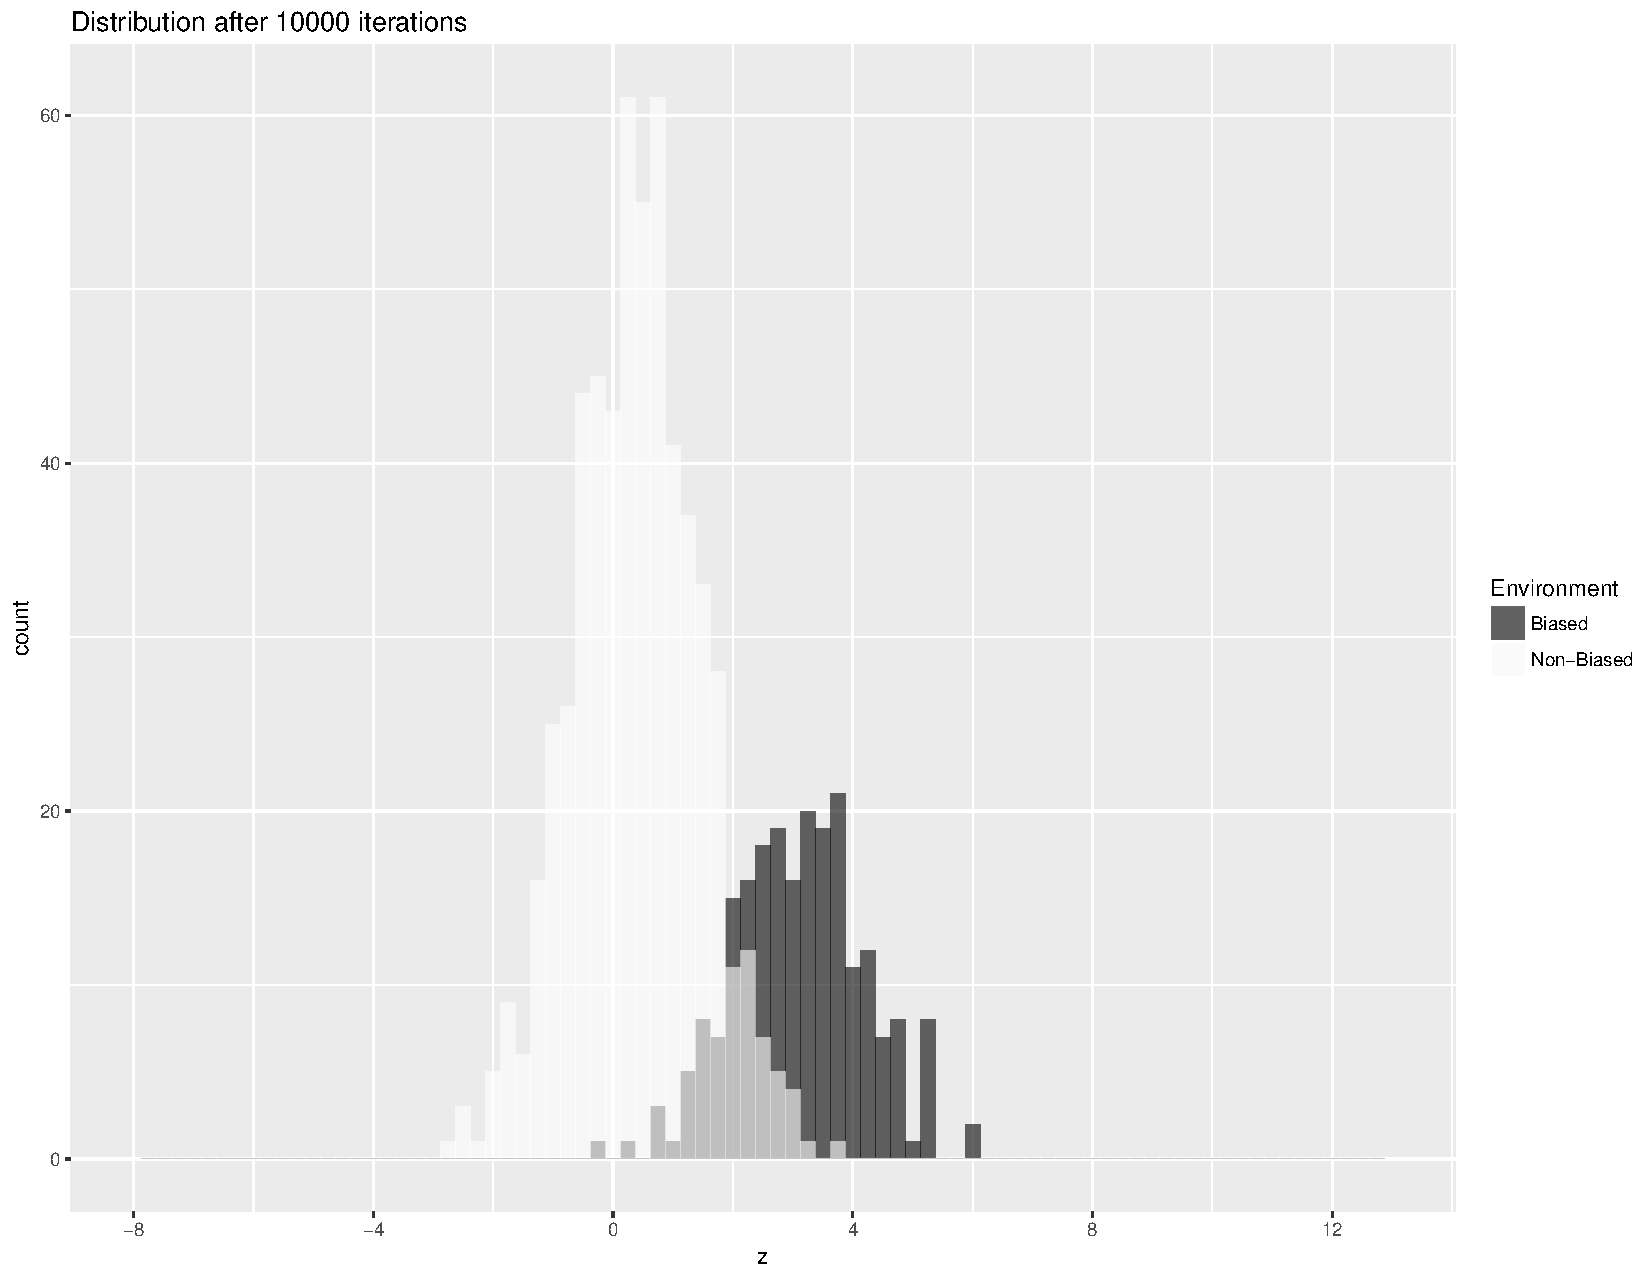
\includegraphics[scale=0.3,bb = 0 0 200 100, draft, type=eps]{BaselineModel10000iter.pdf}\caption{\label{fig:Model2:LengtheningProcess}Soft-Target Model: Increasing
bias function. Single category:Single target. White: tokens produced
in non-biasing contexts. Black: tokens produced in biasing contexts.
x-axis: z-normed \emph{x} dimension. Observation occurs after 10,000
model cycles.}
\end{figure}

For positive \emph{x}, the difference between (\ref{eq:Lengthening Force})
and (\ref{eq:Inertia Force}) is effectively between a monotonically
increasing function with an optimum at 0, and a non-monotonic function
with an optimum at \emph{N}. Theoretically speaking, however, the
former expresses a \textsc{process}, while the latter expresses a
\textsc{state} (cf. \citealt{Hyman1975}). \textsc{process }will be
taken to refer to what would be considered an allophonic rule in generative
phonology, and to which the term `lengthening' (or `shortening') can
properly apply. At the segment level (\emph{S}), the general process
model instantiates the following linguistic relationship: $/S/\rightarrow[S{}^{B}]/$\emph{\_\_B}\textsc{,
}where\emph{ B} stands for the biasing context, and $[S^{B}]$ stands
for the allophonic variant that occurs in that context. Using the
same notation, a \noun{state} model instantiates the following relationship:
$/S^{B}/\rightarrow[S{}^{B}]$ in context \emph{B}. This indicates
that $S^{B}$ is stored, or underlying, rather than generated. A given
\textsc{state} could consist of `long', or `lengthened' tokens, but
does not properly involve `lengthening'. 

\section{\label{sec:Model-Interpretation}Model Space}

The original lengthening model in Chapter \ref{subsec:Phrase-Final Lengthening}
is a \textsc{process} model. As we saw previously, a \textsc{process}
model that lacks a production target is unbounded, producing no stable
outcomes. As will be shown in Section \ref{subsec:Model-B:-Lengthening},
adding a soft target to this model will result in stable outcomes
for a certain range of parameter values. The analogous \textsc{state}
model can be created by implementing the bias term itself as a soft
target, as in (\ref{eq:Length Attractor}) (cf. \citealt{soskuthy2013phonetic}). 

\begin{equation}
L(x_{i})=\alpha(L-x_{i})\label{eq:Length Attractor}
\end{equation}
This model, with one target for non-biased tokens, and one for biased
tokens, can also be shown to produce stable outcomes. The no-target
\noun{process} model, the soft-target \noun{process} model, and the
\noun{state} model, however, differ with respect to their theoretical
consistency, and thus, linguistic interpretability. 

Model 2, from Chapter \ref{subsec:Phrase-Final Lengthening}, re-labelled
as Model A in Table \ref{tab: Model Comparison-1}, is a linguistically
interpretable model. There is a single category from which tokens
are selected at random, either to be produced in biasing contexts,
in which case they are lengthened, or to be produced in non-biasing
contexts, in which case they are unchanged. Model B, with a soft target
at the location of the non-biased, underlying category is also consistent.
All tokens feel a pull towards this underlying target, but those that
happen to be produced in a biasing context are also subject to a force
that lengthens them during production. Model C, however, the \textsc{state}
model, is not theoretically consistent. 

\begin{table}[H]
\caption{Single-Category Model Space\label{tab: Model Comparison-1}}

\noindent\begin{minipage}[t]{1\columnwidth}%
\resizebox{\textwidth}{!}{%
\begin{tabular}{|c||c||c||c||c||c||c|}
\hline 
 & \multicolumn{2}{c||}{} & \multicolumn{2}{c||}{} & Stable & Consistent\tabularnewline
\hline 
\hline 
A & \textsc{Process} & $\alpha(1+x)$ & No Target & – & N & Y\tabularnewline
\hline 
\hline 
B & \textsc{Process} & $\alpha(1+x)$ & Target & $\beta(N-x)$ & (Y) & Y\tabularnewline
\hline 
\hline 
C & \textsc{State} & $\alpha(L-x)$ & Target & $\beta(N-x)$ & Y & N\tabularnewline
\hline 
\end{tabular}

}%
\end{minipage}
\end{table}

In Model C, all tokens have a target at \emph{N}, but tokens produced
in a biasing context have an additional, conflicting target at \emph{L}.
Because there is only a single category in Model C, biased tokens
are generated from the same pool as non-biased tokens, therefore the
second target, \emph{L}, exists without an underlying category with
which that target can be associated. With the distribution initialized
at \emph{N}, the effect is for biased tokens to be moved an arbitrarily
small distance, $\alpha(L-x)$, towards that second target during
production\footnote{As a \noun{process}, incrementality has a straightforward interpretation;
a given token is shifted, or lengthened, by a fixed proportion of
its current length. But in a \textsc{state} model, in which all tokens
are initialized at one target, it is not clear what mechanism would
shift certain tokens only a small amount towards another target. Although,
superficially, this effect is similar to that of the entrenchment
force, $\varepsilon(\overline{x}-x)$, which pushes the tokens of
a given category closer together, they are different in important
ways. The use of the category mean in the entrenchment function stands
in for the sum of the forces that act between individual tokens, maintaining
category cohesion (the same effect can be achieved by averaging over
multiple tokens in production (e.g., \citealt{Pierrehumbert2000,Wedela})).
The soft target, or inertia force, on the other hand, references a
fixed target location that is specified independently of the current
distribution. }. Of the three models, only Model B is both stable (bounded), and
theoretically consistent. 

Model C, however, can be made theoretically consistent by introducing
a second level of representations. If the parent category can be split
into two sub-categories, then each target can be associated with a
different sub-category. This is Model G in Table \ref{tab: Model Comparison},
which is the 2-level model analog of Table \ref{tab: Model Comparison-1}.
The remaining models in this table are all theoretically problematic
in different ways. Model D is the two sub-category counterpart of
Model B. while Model B was theoretically consistent, the introduction
of a separate sub-category for biased tokens in Model D creates a
representational paradox: a category with no target, to which lengthening
continuously applies. Model D is also unbounded. Model E re-creates
the two-target paradox of Model C. And F is the hybrid \noun{process}+\emph{state}
model\footnote{If double specifications are possible (e.g., \textsc{process} + \textsc{state}),
then the total set of possible models includes the Single-Category
\textsc{process}+\textsc{state} model, and the set of non-biased No-Target
models, among others. However, these other models all contain a superset
of the representational inconsistencies already described, and therefore
are not included.}.

\begin{table}[H]
\caption{2-Level Model Space\label{tab: Model Comparison}}

\noindent\begin{minipage}[t]{1\columnwidth}%
\resizebox{\textwidth}{!}{%
\begin{tabular}{|c||c||c||c||c||c||c|}
\hline 
 & \multicolumn{2}{c||}{biased} & \multicolumn{2}{c||}{non-biased} & Stable & Consistent\tabularnewline
\hline 
\hline 
D & \textsc{Process} & $\alpha(1+x)$ & Target & $\beta(N-x)$ & N & N\tabularnewline
\hline 
\hline 
E & \textsc{2-State} & $\beta(N-x)$; $\alpha(L-x)$ & Target & $\beta(N-x)$ & Y & N\tabularnewline
\hline 
\hline 
F & \textsc{Process+ State} & $\alpha(1+x)$; $\alpha(L-x)$ & Target & $\beta(N-x)$ & Y & N\tabularnewline
\hline 
\hline 
G & \textsc{State} & $\alpha(L-x)$ & Target & $\beta(N-x)$ & Y & Y\tabularnewline
\hline 
\end{tabular}

}%
\end{minipage}
\end{table}

Only two viable candidates emerge from the full set of models. A pure
\textsc{process} model with a single target (B), and a pure \textsc{state}
model (G). In general terms, these results show us that \textsc{process}
and \textsc{state} models are incompatible with one another. If biased
tokens have a separate representational status, this implies that
only tokens from this sub-category should be chosen to be produced
in biased contexts. Furthermore, since the biased sub-category has
a target at \emph{L}, those tokens will already be appropriately longer
than their non-biased counterparts (with a target at \emph{N}). Therefore,
there is no motivation for lengthening them further. Effectively,
this would be equivalent to a phonological rule of the form:
\begin{covexamples}
\item \label{Process-+-State:}Process + State: $/S^{B}/\rightarrow[S{}^{B^{B}}]/$\emph{\_\_B}
\end{covexamples}
Although (\ref{Process-+-State:}) is linguistically ill-formed, it
is equivalent to the feedback loop at the heart of the basic exemplar
model\footnote{It should be noted that, as far as I am aware, no one has actually
proposed the context-dependent exemplar models in Chapter \ref{sec:The-Exemplar-Model}.
They are what I take to be the logical extension of the context-free
exemplar model of \citet{Pierrehumbert2000}.}. Cumulativity of small differences is only possible if the bias effects
in production (contextually determined allophony) are stored (\noun{state}),
rather than being stripped away during perception. Storage of allophonic
detail implies that the biasing context itself is discarded, or at
least not used to recover the underlying form. In production, however,
the \textsc{process} model requires knowledge of the context that
triggers biasing. In other words, the allophonic rule is available
in production, but not in perception\footnote{The alternative is that both the unnormalized surface forms, and their
production context are stored, or incorporated into the category label
in some way. Even if so, it is still not clear why an allophonic rule
would continue to apply. Furthermore, if prior specification of complex
sub-structure is required (and, in the limit, a unique category for
every token) the exemplar framework does not seem to offer much, if
anything, in terms of explanatory power. }. 

Another way to characterize this theoretical incompatibility is that
a \textsc{process} model implies that normalization takes place, while
a \textsc{state} model implies that it does not. Thus, inconsistency
results when either the production or perception stage of a given
model assumes normalization, while the other doesn't. In the Pure
Process Model (B), all tokens are drawn from the same distribution
in production, with a target, or underlying specification, at \emph{N}.
Lengthening applies as an allophonic rule, but in perception all tokens
are drawn back to the same underlying target at \emph{N}, whether
they are lengthened or not. Thus, the inertial force acts to partially
normalize the effect of lengthening. Complete normalization (fixed
target) would prevent change entirely. In the Pure State Model (G),
on the other hand, normalization fails to occur in the sense that
`lengthened' tokens are assigned to their own sub-category, and no
allophonic rules apply. Again, the \textsc{state} aspect is only partial.
The fact that these are sub-categories rather than completely independent
categories introduces a connection between the biased and non-biased
tokens which implies that the relationship between them is known,
and therefore, that the allophonic transformation is known. Two entirely
independent categories would preclude change entirely. 

\section{\label{sec:Model-Behavior}Consistent and Convergent Models of Sound
Change}

This section is devoted to an exhaustive analysis of the ends states
of the two theoretically consistent and bounded models: the Pure Process
Model (B), and the Pure State Model (G). These results will be provided
in the form of two parameters: the category means along the dimension
\emph{x}, and the difference between the means of the biased and non-biased
sub-distributions. Because it is not possible to guarantee that simulations
will fully sample the space of possible outcomes, stable states will
be explicitly derived as a function of model parameters. The derivation
will be given in abbreviated terms in the text, with the full details
provided in the appendices. Following \citet{soskuthy2013phonetic,Soskuthy2015},
the percentage of tokens produced in a biasing context (bias proportion)
will act as the independent variable. The term “attractor” will
also be adopted in reference to a soft target, in order to facilitate
comparison to that work. 

\subsection{\label{subsec:Lengthening-as-State}State Model: Sub-categories}

The Pure State Model contains one target for biased tokens, and a
distinct target for non-biased tokens. Figure \ref{fig:Model G} provides
an illustration of the forces acting at some model time \emph{t},
on exemplar categories modeled as Normal functions. As will be shown
below, the means of both sub-categories can be guaranteed to lie somewhere
between the two targets at \emph{N} and \emph{L}. Each sub-category
is subject to the inertia associated with its own target, acting to
pull the two apart. Membership in a superset category is implemented
via the entrenchment force, which pulls both in the direction of the
global mean, and thus towards one another\footnote{\citet{soskuthy2013phonetic} links sub-categories by applying phonetic
biasing probabilistically to both, but with the biased sub-category
more strongly weighted. }. In this illustration, the relative number of tokens produced in
biasing versus non-biasing contexts is represented by the heights
of the Normal curves. Because the proportion of biasing contexts is
less than 50\% in this example, the global mean (indicated by the
dashed line) is closer to the mean of the non-biased distribution. 

\begin{figure}[H]
\begin{centering}
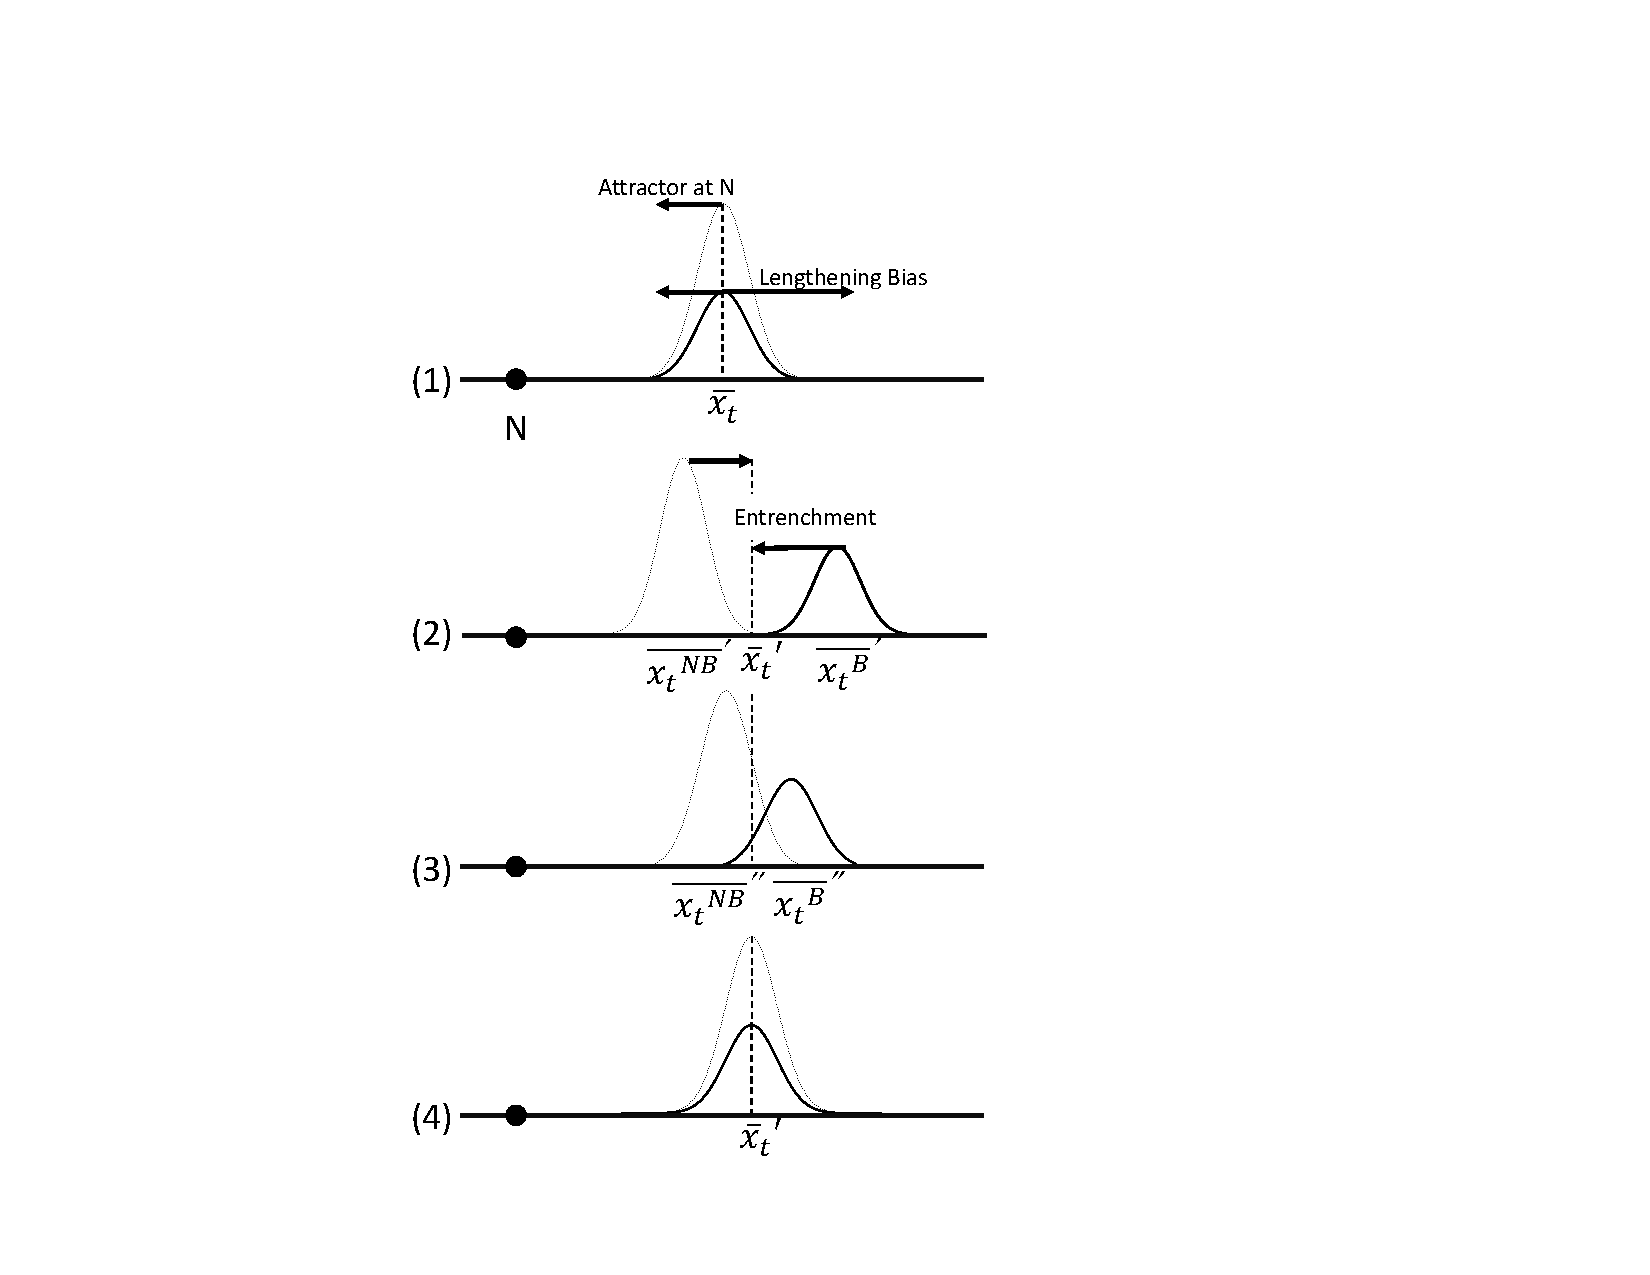
\includegraphics[scale=0.5,bb = 0 0 200 100, draft, type=eps]{Model6Behavior.pdf}\caption{\label{fig:Model G}Schematic of forces for Pure State Model}
\par\end{centering}
\end{figure}

The equations for each of the model forces have been given previously,
but are repeated here for ease of reference: (\ref{eq:Entrenchment-2})
Entrenchment, (\ref{eq:Inertia-2}) Inertia (attractor) at \emph{N},
and (\ref{eq:Length Attractor-2}) Inertia (attractor) at\emph{ L}.
A small random error term is also included in all models. 

\begin{equation}
E(x_{i})=\epsilon(\bar{x}-x_{i})\label{eq:Entrenchment-2}
\end{equation}

\begin{equation}
I(x_{i})=\beta(N-x_{i})\label{eq:Inertia-2}
\end{equation}

\begin{equation}
L(x_{i})=\alpha(L-x_{i})\label{eq:Length Attractor-2}
\end{equation}
In order to estimate the behavior of this model under various conditions
we will make the simplifying assumption that each sub-category is
specified by a Normal curve with variable mean, but fixed standard
deviation. This allows us to use the mean of each sub-category as
a proxy for its global behavior. To determine the stable model outputs,
we use the fact that forces must balance at this equilibrium point,
meaning that no further changes occur in the location of the means.
Therefore, the sum of all forces is set to zero. $\overline{x_{E}}$
is defined as the location of the global mean at equilibrium, while
$\overline{x_{E}^{B}}$ and $\overline{x_{E}^{NB}}$ are the equilibrium
means of the biased and non-biased sub-categories, respectively. 

The first step is to prove that there is no way for the mean of either
sub-category (and therefore, the global mean) to have a value less
than \emph{N}, or greater than \emph{L}. This follows from the mathematical
form of the inertial, or attractor, forces. For values greater than
the attractor location, the force is leftward, but for values smaller
than the attractor location, the force is rightward, thus always acting
to push the distribution precisely to the attractor location. If the
sub-categories were completely independent (no global entrenchment),
then they would always stabilize at their respective attractor locations.
Entrenchment allows the sub-categories to be perturbed from their
attractors, but only in the direction of the other sub-category. Thus,
we can be confident that they will end up at equilibrium somewhere
between \emph{N} and \emph{L}. The exact location will depend on the
parameters $\alpha$ (the strength of the attractor at \emph{L}),
$\beta$ (the strength of the attractor at \emph{N}), $\varepsilon$
(the strength of the entrenchment force), and $p$ (the bias proportion:
the percentage of the category consisting of biased tokens; in other
words, the percentage of tokens produced in a biasing context). 

The equilibrium location for the non-biased sub-category is determined
by the point at which global entrenchment (\ref{eq:Entrenchment})
is perfectly balanced by the attractor at \emph{N} (\ref{eq:Inertia Force}).
Using the equilibrium location of the mean to stand in for the entire
sub-category: $\beta(N-\overline{x_{E}^{NB}})+\varepsilon(\overline{x_{E}}-\overline{x_{E}^{NB}})=0$.
Therefore, $\beta(\overline{x_{E}^{NB}}-N)=\varepsilon(\overline{x_{E}}-\overline{x_{E}^{NB}})$.
For the biased distribution, it is the attractor at \emph{L} (\ref{eq:Length Attractor})
that will be balanced by global entrenchment (\ref{eq:Entrenchment}):
$\alpha(\overline{x_{E}^{B}}-L)=\varepsilon(\overline{x_{E}}-\overline{x_{E}^{B}})$.
In order to solve for the three quantities, $\overline{x_{E}^{B}}$,
$\overline{x_{E}^{NB}}$ , and $\overline{x_{E}}$ , we need a third
equation linking them. This is given by the equation that expresses
the global mean as a weighted average of the two sub-category means.

\begin{equation}
\overline{x_{E}}=(1-p)\overline{x_{E}^{NB}}+p\overline{x_{E}^{B}}\label{eq:weighted mean}
\end{equation}
We can now solve for each of the quantities in turn by substitution.
Appendix C shows the full derivation, and demonstrates that the global
mean at equilibrium, $\overline{x_{E}}$ , can be expressed in the
following terms:

\begin{equation}
\overline{x_{E}}=\frac{(1-p)\beta N(\alpha+\varepsilon)+p\alpha L(\beta+\varepsilon)}{(\beta+\varepsilon)(\alpha+\varepsilon)-(\alpha+\varepsilon)(1-p)\varepsilon-(\beta+\varepsilon)p\varepsilon}\label{eq: sub-dist}
\end{equation}
as a function of the set of model parameters ($\alpha,\beta,N,L,p$),
the location of the global mean at equilibrium. The other quantity
of interest is the distance between the sub-category means, which
can be expressed as a function of $\overline{x_{E}}$ :
\begin{equation}
\Delta\overline{x_{E}}\equiv\overline{x_{E}^{B}}-\overline{x_{E}^{NB}}=\frac{\alpha L+\varepsilon\overline{x_{E}}}{\alpha+\varepsilon}-\frac{\beta N+\varepsilon\overline{x_{E}}}{\beta+\varepsilon}\label{eq:State Model-sep}
\end{equation}
Keeping all other variables constant, we can now derive the behavior
of these two quantities as a function of the bias proportion, \emph{p}. 

The change in $\overline{x_{E}}$ that results from a change in \emph{p}
is given by taking the partial derivative of Eq. (\ref{eq: sub-dist}).
This turns out to be somewhat unwieldy to calculate in general form.
In the special case when all forces have the same strength ($\alpha=\beta=\varepsilon$),
we can show that Eq. (\ref{eq: sub-dist}) reduces to $\overline{x_{E}}=N+p(L-N)$.
Therefore, the global category mean is a positive linear function
of \emph{p}, and the change in the location of that mean is constant:
$\frac{\partial\overline{x_{E}}}{\partial p}=L-N$. 

For other cases, it's possible to determine the general behavior of
$\frac{\partial\overline{x_{E}}}{\partial p}$ even without an exact
solution. Assume that the equilibrium state for a given $p=p_{j}$
has already been determined. Now increase \emph{p} to $p_{k}$. Eq.
(\ref{eq:weighted mean}) entails that if $p_{k}>p_{j}$ (an increase
in bias proportion), then the global mean will shift closer to the
biased sub-category. Because the strength of the entrenchment force
depends on the distance from the global mean, this shift will, in
turn, cause the entrenchment force on the non-biased sub-category
to increase. Because the attractor at \emph{N} and the entrenchment
force are taken to be perfectly balanced at $p=p_{j}$, an increase
in the latter will result in a shift of the non-biased sub-category
toward the biased one. At the same time, the entrenchment force on
the biased sub-category will decrease commensurately. In this case,
a decrease in the entrenchment force causes the balance to shift in
favor of the attractor at \emph{L}, meaning the biased sub-category
will also shift in the rightward direction. Because the sub-categories
shift in the same direction, the equilibrium point for the global
mean is also guaranteed to shift in that direction, and thus to increase
as \emph{p} increases: $\frac{\partial\overline{x_{E}}}{\partial p}>0$. 

In the special case where $\alpha=\beta=\varepsilon$, we can use
the result that $\frac{\partial\overline{x_{E}}}{\partial p}=L-N$,
and determine that $\frac{\partial\Delta\overline{x_{E}}}{\partial p}=0$.
Therefore, the distance between the two sub-categories remains constant
in this case. The general form of the partial derivative of (\ref{eq:State Model-sep})
with respect to \emph{p,} $\frac{\partial\Delta\overline{x_{E}}}{\partial p}$,
can be written as a function of the partial derivative of $\overline{x_{E}}$
with respect to \emph{p} ($\frac{\partial\overline{x_{E}}}{\partial p}$):
\begin{equation}
\frac{\partial\Delta\overline{x_{E}}}{\partial p}=\frac{\partial\overline{x_{E}}}{\partial p}\varepsilon[\frac{1}{\alpha+\varepsilon}-\frac{1}{\beta+\varepsilon}]\label{eq: Model G: dsep/dp}
\end{equation}
Since we know that $\frac{\partial\overline{x_{E}}}{\partial p}$
is always positive, the sign of $\frac{\partial\Delta\overline{x_{E}}}{\partial p}$
is determined by the sign of $\frac{1}{\alpha+\varepsilon}-\frac{1}{\beta+\varepsilon}$.
The sign of $\frac{1}{\alpha+\varepsilon}-\frac{1}{\beta+\varepsilon}$
is determined by the relative sizes of the quantities $\alpha+\varepsilon$,
and $\beta+\varepsilon$. Therefore, if $\alpha>\beta$ then $\frac{\partial\Delta\overline{x_{E}}}{\partial p}<0$;
and if $\alpha>\beta$ , then $\frac{\partial\Delta\overline{x_{E}}}{\partial p}<0$.

\subsection{\label{subsec:Model-B:-Lengthening}Process Model: Single Category}

The Pure Process Model contains a single category, and a single target
for that category. Tokens are selected at random, with probability
\emph{p,} to be produced in the biasing context. This model is identical
to the Soft Target Model described in Section \ref{subsec:Soft-Targets}
(Fig. \ref{fig:Model2:LengtheningProcess}). It will be shown in this
section that the Process Model is only stable for certain parameter
values. The behavior of the global mean, and the average separation
between biased and non-biased productions, will be derived as before.
The same simplifying assumption that the category can be approximated
as a Normal distribution with fixed variance will also be made. However,
it should be noted that this assumption is less justified for the
one-category model due to the fact that biased and non-biased variants
will separate, creating a lumpier distribution, and likely an increase
in variance.

The derivational steps in this analysis are given graphically in Fig.
\ref{fig:Derivation}. Panel 1 is a snapshot of the model at some
time, \emph{$t$}, when the global mean is located at location $\overline{x_{t}}$
along \emph{x}. Both biased and non-biased tokens are sampled from
this distribution, at different rates. This relationship is indicated
by the darker normal curve (subset of tokens subjected to bias during
production) within the lighter one (subset of tokens non-biased during
production). 

\begin{figure}[H]
\centering{}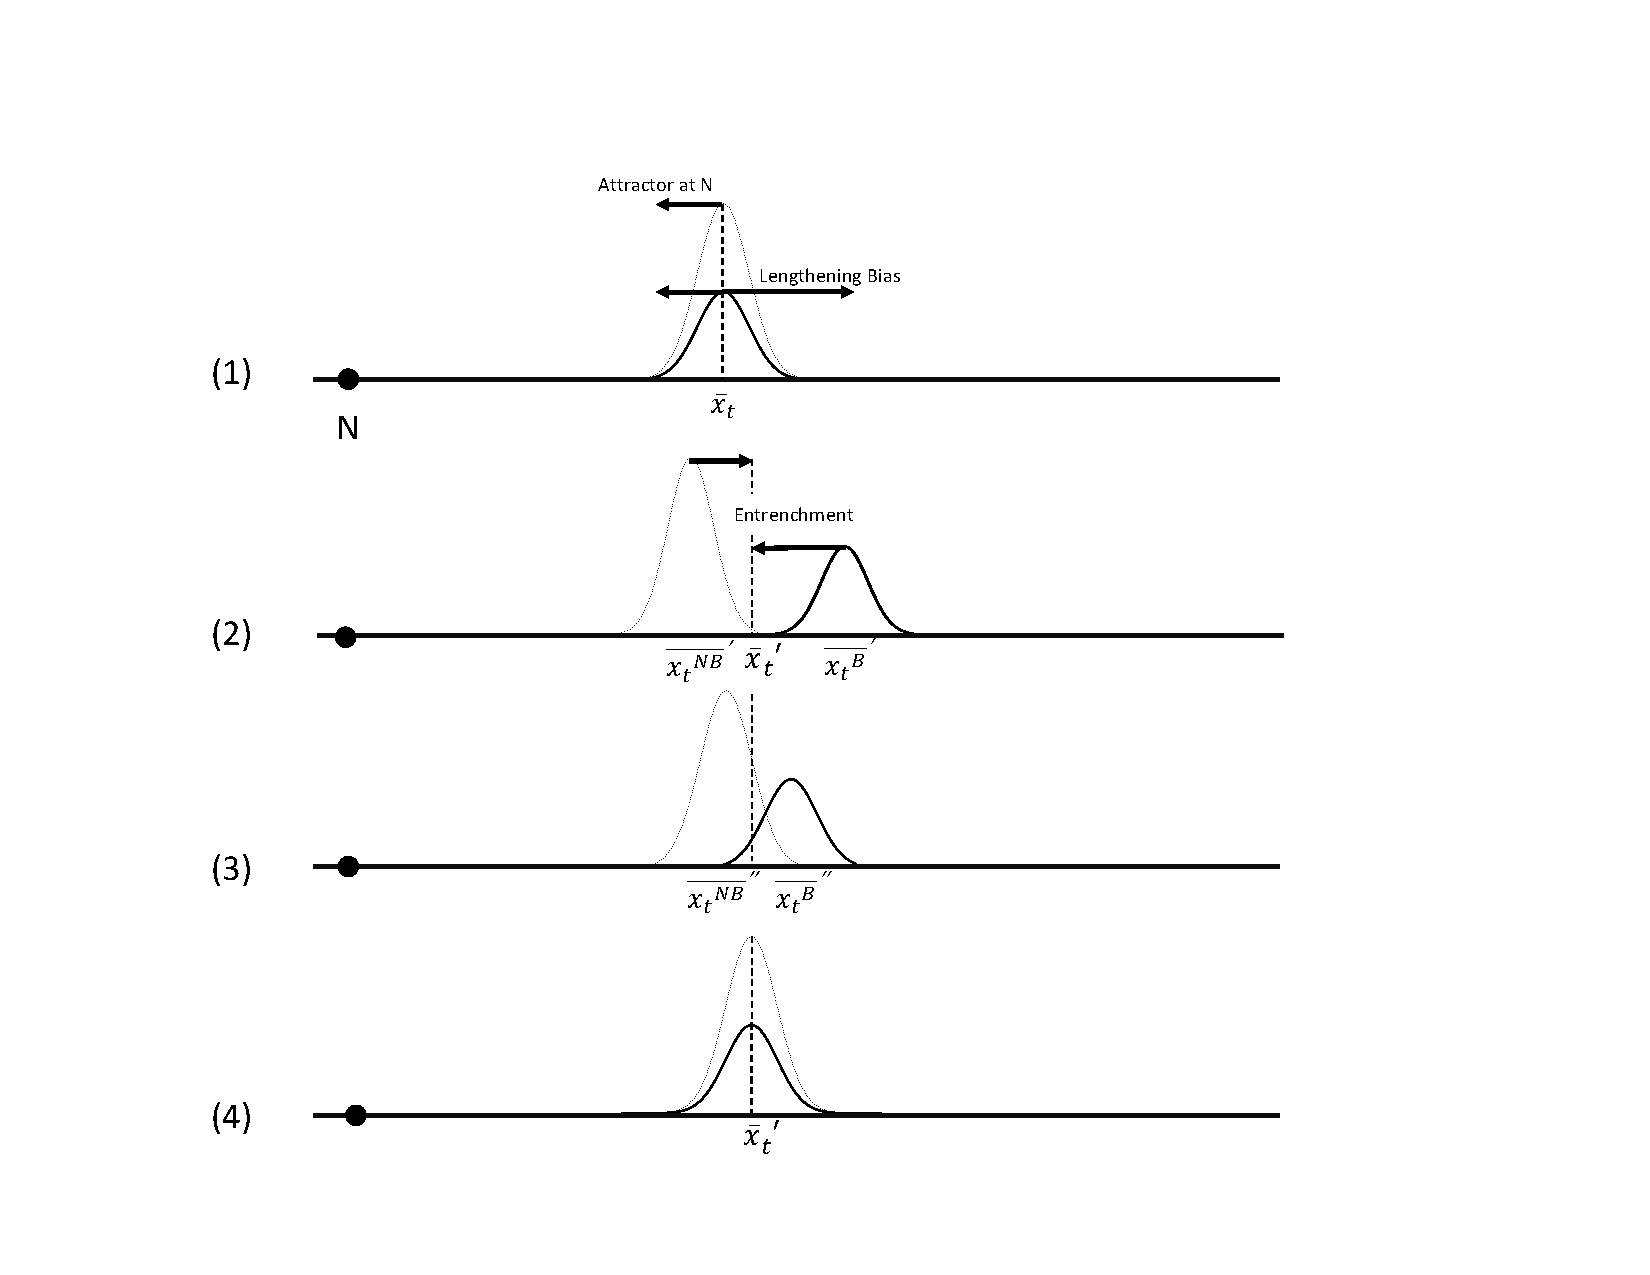
\includegraphics[width=0.75\paperwidth,bb = 0 0 200 100, draft, type=eps]{Model1Behavior.pdf}\caption{\label{fig:Derivation}Schematic of forces for \noun{process} model}
\end{figure}

The production value of any token at any time \emph{t} can be calculated,
as long as its current value, and the category mean, are known. All
tokens are subject to the attractor at \emph{N}. And all tokens are
subject to the entrenchment force acting to pull them closer to the
current category mean (which will be greater than, or equal to, \emph{N}).
Additionally, a proportion \emph{p} of randomly selected tokens undergo
a lengthening process, moving away from the rest of the distribution
during production.

Panels 2-4 of Fig.\ref{fig:Derivation} take us sequentially through
the application of forces. Panel 2 isolates the effect of applying
the attractor and lengthening forces. The attractor affects all tokens
equally, because all tokens are equally far from \emph{N} on average.
Lengthening, applied only to a subset of tokens, splits the distribution
apart. Before entrenchment applies, the mean values for the observed
productions ($\overline{x_{t}^{B}}^{\prime}$, mean of biased productions
in Panel 2; $\overline{x_{t}^{NB}}^{\prime}$ mean of non-biased productions
in Panel 2), can each be given as a function of the global mean at
time $t$, $\bar{x_{t}}$:

\begin{equation}
\overline{x_{t}^{B}}^{\prime}=\bar{x_{t}}(1+\alpha)+\beta(N-\bar{x_{t}})\label{eq:Biased}
\end{equation}

\begin{equation}
\overline{x_{t}^{NB}}^{\prime}=\bar{x_{t}}+\beta(N-\bar{x_{t}})\label{eq:Non-biased}
\end{equation}
Applying entrenchment does not affect the global mean, only the absolute
locations of the sub-distribution means, and their separation. Therefore,
the mean in Panel 3 is identical to the mean from Panel 2. This mean
($\bar{x_{t}}^{\prime}$) is given by the weighted average of the
means of the observed production variants: 

\begin{equation}
\bar{x_{t}}^{\prime}=(1-p)\overline{x_{t}^{NB}}^{\prime}+p\overline{x_{t}^{B}}^{\prime}\label{eq: G weighted mean}
\end{equation}
Equilibrium is achieved when continued iterations fail to change the
locations of the means. This means that they should be unaffected
by successive iterations of biasing. $\overline{x_{E}}^{\prime}=\overline{x_{E}}$
, $\overline{x^{B}}^{\prime}=\overline{x^{B}}$, and $\overline{x^{NB}}^{\prime}=\overline{x^{NB}}$.
Therefore, 

\begin{equation}
\overline{x_{E}}=(1-p)\overline{x_{E}^{NB}}^{\prime}+p\overline{x_{E}^{B}}^{\prime}\label{eq:equilbrium 1}
\end{equation}
and from Eq. (\ref{eq:Biased}) and (\ref{eq:Non-biased}), 

\begin{equation}
\overline{x_{E}}=(1-p)\{\overline{x_{E}}+\beta(N-\overline{x_{E}})\}+p\{\overline{x_{E}}(1+\alpha)+\beta(N-\overline{x_{E}})\}\label{eq:equilbrium 2}
\end{equation}
Solving for $\overline{x_{E}}$ gives

\begin{equation}
\overline{x_{E}}=\frac{\beta N}{\beta-p\alpha}\label{eq: lengthening process}
\end{equation}
See Appendix \ref{chap:Appendix D} for the full derivation. 

The behavior of the global mean as a function of \emph{p} will depend
on which region of parameter space we are in: $p\alpha<\beta$, or
$p\alpha>\beta$. For $p\alpha<\beta$, the denominator in (\ref{eq: lengthening process})
is positive. Therefore, as \emph{p} increases (but $p\alpha$ stays
smaller than $\beta$), the denominator decreases, and the global
mean increases ($\frac{\partial\overline{x_{E}}}{\partial p}>0$).
In the limit, as $p\alpha$ goes to $\beta$, the equilibrium mean
goes to infinity, and lengthening is unbounded. For $p\alpha>\beta$
, the denominator is negative, which also means that the mean is negative,
and the only equilibrium point is negative. Since negative duration
values aren't possible, there is no well-defined equilibrium in the
range in which $p\alpha>\beta$. The \noun{process} model is thus
only stable if the lengthening strength ($\alpha$) is not too great,
and the percentage of biasing contexts ($p$) is not too large, relative
to the attractor strength ($\beta$).

To calculate the second quantity of interest: the dependence of sub-distribution
separation on \emph{p,} the effect of entrenchment must be included.
Entrenchment acts to bring all tokens back towards the global mean
by an amount proportional to their distance from that mean (Panel
3 of Fig. \ref{fig:Derivation}): 

\begin{equation}
\overline{x^{B}}^{\prime\prime}=\overline{x^{B}}^{\prime}+\varepsilon(\overline{x}^{\prime}-\overline{x^{B}}^{\prime})\label{eq:Panel 3 biased}
\end{equation}

\begin{equation}
\overline{x^{NB}}^{\prime\prime}=\overline{x^{NB}}^{\prime}+\varepsilon(\overline{x}^{\prime}-\overline{x^{NB}}^{\prime})\label{eq:Panel 3 unbiased}
\end{equation}
The separation between the two production variants after entrenchment
applies ($\triangle\overline{x}^{\prime\prime}$) can be determined
by taking the difference between Equations (\ref{eq:Panel 3 biased})
and (\ref{eq:Panel 3 unbiased}): 

\begin{equation}
\triangle\overline{x}^{\prime\prime}\equiv\overline{x^{B}}^{\prime\prime}-\overline{x^{NB}}^{\prime\prime}=(1-\varepsilon)(\overline{x^{B}}^{\prime}-\overline{x^{NB}}^{\prime})
\end{equation}
The final separation depends only on the separation prior to the application
of entrenchment ($\triangle\overline{x}^{\prime}$ in Panel 2), and
the strength of the entrenchment term, $\varepsilon$. Because the
sub-distributions only exist at production, no cumulativity in separation
is possible (see Panel 4). Therefore, at all times \emph{t}, the separation
in Panel 2, prior to entrenchment, will always be given by the lengthening
factor: $\alpha\overline{x_{t}}$. Therefore, at equilibrium, when
$\overline{x_{t}}=\overline{x_{E}}$, the average distance between
the two production sub-distributions is given by

\begin{equation}
\varDelta\overline{x_{E}}=(1-\epsilon)(\alpha\overline{x_{E}}).\label{eq:Cat Sep}
\end{equation}
In the stable parameter range ($p\alpha>\beta$), where $\overline{x_{E}}$
increases as \emph{p} increases, the separation of the sub-distributions
also increases, but more slowly, by a factor of $(1-\epsilon)\alpha$.

\section{\label{sec:Actuation}Change between Stable States}

Most work in the exemplar framework models either change or stability,
but not both. That is to say, only one stable state is possible, and
the model either starts in that state, in which case it remains there
for all time, or inevitably arrives in that state from any other starting
conditions. In \citet{Garrett2013} there are two different modes
of processing\footnote{These are likened to “speech” and “non-speech” processing
modes (\citealt{liberman1967perception}); individual speakers may
switch between the two modes, or different speakers may operate consistently
in one or the other mode (e.g. \citealt{yu2013socio}). }, resulting in essentially two different models: one in which normalization
occurs, which is stable, and one in which normalization is “turned
off”, leading to change (the latter model is not implemented, but
would lead to unbounded shift without an additional mechanism). \citet{Kirby2014}
is similar in that two different outcomes are possible, one for a
`misparsing' mode, and one for accurate parsing (In the `misparsing'
mode, merger is prevented by a stage of hypothesis selection in which
a Bayesian learner updates phonetic cue weights so as to optimize
categorization accuracy). 

“Agent-based” models (not all implemented using exemplar representations)
use the interaction among one or more groups of speakers to be the
driving mechanism, either of the evolution of language itself, or
of the evolution of pre-existing variants (which may be parameters,
or entire grammars). Systems are taken to be stable within individual
speakers, that is, without bias. Thus there is no mechanism via which
a truly novel form can arise, only ways in which an existing distribution
can evolve within a heterogeneous population (\citealt{Niyogi1997,Boer2000,nowak2001evolution,Steels2005,baxter2006utterance,oudeyer2006self,fagyal2010centers,stanford2013revisiting,pierrehumbert2014model}).
Models that rely on simple `self-organizing' principles, such as random
selection, or mis-classification, are usually designed to demonstrate
that a single optimal state will be reached from any starting position
(\citealp{Wedela,ettlinger2007exemplar,Wedel2006,Blevins2009,DBLP:journals/corr/Tupper14a,wedel2017category}).
Some additional mechanism would be needed to change such systems further.
Effectively, actuation is achieved either through speaker contact
(in which adoption of already existing variants may occur), or by
initializing the model in an unstable state. 

As far as I am aware, \citet{soskuthy2013phonetic} and \citet{Soskuthy2015}
are unique in the literature in that they capture both change and
stability within a single model. Actuation occurs via a completely
speaker-internal mechanism that is an integral component of the model:
allophone frequency. Model 1 in Chapter \ref{subsec:Model-1:-Context-Free}
was an instantiation of frequency of use as an instigator of change,
in the successive reduction of highly frequent words. In that model,
frequency was a fixed property of a given word type. But changes in
word frequency, as well as in the relative proportion of contextual
variants, are possible for independent reasons. Words go in and out
of style, and the frequency of use of any given word is expected to
change over time. In turn, changes in frequency at the word level
also affect the frequency of occurrence of the phonemes that make
up the word. For changes that happen to affect a group of words with
the relevant allophonic environment, a change in token proportion
between multiple allophones of a given phoneme could result. 

The model of vowel lengthening in \citet{soskuthy2013phonetic} was
the basis for the gradient context-dependent model first introduced
in Chapter \ref{sec:Context-Dependent-Iterativity}. This model was
gradually developed, first into a set of possible models implementing
at least one soft target, then into a subset of those that were both
stable and theoretically consistent. The remaining two models were
then implemented with frequency of allophonic environment (bias proportion)
as the actuator of change. \citet{soskuthy2013phonetic} is actually
closest to Model E (Section \ref{sec:Model-Interpretation}), as a
two-target \noun{state} model. The vowel-level category is modeled
as a mixture of Gaussians, namely the sub-category of variants that
occur in the lengthening context, and the sub-category of variants
that occur in the non-lengthening context. Instead of global entrenchment,
the link to the superset category is implemented by applying lengthening
stochastically to tokens chosen from both sub-categories, but with
the `long' sub-category more strongly weighted. Additionally, a “centering
bias”, implemented as an attractor at \emph{N}, is used to prevent
unbounded dispersion\footnote{This is necessary to counteract the contrast maintenance pressure
that pushes categories away from one another, via elimination of ambiguous
tokens (\citet{Wedel2008} and \citet{Blevins2009}). }. The mathematical form of the attractor function is equivalent to
the soft target first introduced in Section \ref{subsec:Soft-Targets}:
an inertial force that applies when tokens are perturbed from an underlyingly
specified position, acting to pull them back towards that position.
This results, functionally, in two targets for the biased sub-category
(one at \emph{N} and one at \emph{L})\footnote{\citet{Soskuthy2015} employs a similar architecture. There is an
explicit target for only the biased sub-category, but all tokens are
affected by the same centering force. In this model, hard thresholds
at 0 and 1 act to force both distributions back towards the center,
similarly to how a target attracts tokens from either direction. These
attractors are critical to achieving stable states in both models.}. 

Sóskuthy's model therefore differs from the Pure State Model implemented
in Section \ref{subsec:Lengthening-as-State}. The actual model behavior,
however, turns out to be quite similar. As we saw in the previous
section, changes in bias proportion – how often the biasing context
occurs relative to the non-biasing context – act to shift the model
from one stable state to another. The global mean of the vowel category
always increases with increasing \emph{p}, but the separation between
the `lengthened' and `unlengthened' variants can increase, decrease,
or stay the same, depending on other model parameters\footnote{In Sóskuthy's models there is a somewhat more complex dependence on
\emph{p}. }. Under the assumption that parameter values are fixed within a given
speaker, only one of those outcomes will actually be possible for
each individual. 

\section{\label{subsec:Phoneme-Split}Phoneme Split}

Existing exemplar models of change are actually models of phonetic,
rather than phonological, change. The framework offers the possibility
that low-level synchronic variation, like phonetic nasalization, can
successively accumulate, leading to large-scale change. However, the
basic framework does not, in and of itself, offer a solution to the
actuation problem at the phonological level. We know that new phonological
categories can form over time, and this seems to happen when phonetic
allophones achieve independence from their parent categories. Thus,
the outcome in which lengthened vowels become contrastive long vowels,
and nasalized vowels become contrastive nasal vowels, is of particular
interest. It has been proposed that phoneme genesis is triggered by
a subset of phonetic variants that have shifted sufficiently far from
the rest of the distribution (\citealt{Janda2003,Janda2008}). This
is essentially what is assumed in \citet{Wedel2008}, with phonemic
contrast equated to the emergence of a bi-modal distribution. However,
as we saw in the \noun{state} model of Section \ref{subsec:Lengthening-as-State},
`long' tokens can never get longer than their attractor at \emph{L},
and the distance between the two sub-categories is similarly constrained
by the distance between the two attractors. This is problematic if
phonetic exaggeration or “enhancement” is necessary to initiate
a new phonological category. The \noun{process} model seems to offer
more potential for phonological change if lengthening can be somehow
turned off right after biased tokens achieve sufficient separation
from the non-biased part of the distribution. In fact, what is needed
to model phoneme split with the current set of models is precisely
a mechanism that will enact the necessary representational changes
needed to convert a \noun{process} model (allophony) to a \noun{state}
model (contrast)\footnote{Going from a \noun{state} to a \noun{process} model, on the other
hand, requires that independent categories become linked through the
inference of a predictable relationship between them. In one sense,
phoneme merger is clearly the opposite of phoneme split in that the
former reduces the number of independent categories, while the latter
increases them. However, phoneme merger is not equivalent to (re-)establishing
an allophonic relationship. As far as I am aware, merger is taken
to be the result of phonetic overlap among distinct categories (that
may or may not share allophones) involving the wholesale replacement
of one category with another occupying the exact same phonetic space.
A change from a \noun{state} to a \noun{process} therefore, may be
a different kind of change, and perhaps one that has no exact correspondent
in the standard taxonomy of sound change. This is an intriguing avenue
for future work.}.

In addition to the question of how the transition from \noun{process
}to\noun{ state} can occur, there is the separate question of the
level at which the \noun{state} is specified. Features, such as {[}\emph{voice}{]},
or {[}\emph{nasal}{]}, are usually considered to be the universal
atoms from which all phonemes are constructed. However, a given rule,
or process, acts over some set of phonemes within a given language.
Each individual phoneme consists of a unique matrix of feature values,
but the phoneme class is specified by the subset of feature values
that all members share (comprising a natural class). In principle,
any combination of feature values for any subset of features could
be a natural class that is linguistically relevant in some language.
Yet the number of such classes that are actually used, or active,
within a given language is much smaller. Furthermore, the existence,
or activity, of a particular natural class within a language is identified
only by the fact that all and only the phonemes that belong to that
class behave identically with respect to some rule. It is uncontroversial
that the rule must be learned by the speaker of the language, and
therefore, which natural class is associated with the rule must also
be learned. Thus, it is not unlikely that the natural class itself
is learned, or formed, at the time the rule is learned. This view
is further supported by the possible existence of “unnatural”
classes (e.g., \citealt{Mielke2008}).

In the case of vowel lengthening, the relevant class of segments that
undergo the rule consists of the natural class that specifies all
and only vowels. The class of segments that act as the trigger, or
environment, for the rule is the set of all non-continuant non-nasal
voiced segments. In both the \noun{state} and \noun{process} models
this sub-category is explicitly represented, and in fact, the models
are initialized with this representation\footnote{It is worth noting that {[}\emph{vowels before everything else}{]}
does not actually comprise a natural class due to its disjoint nature,
consisting of the union of the following natural classes: {[}\emph{vowels
before continuant}s{]}, {[}\emph{vowels before nasals}{]}, and {[}\emph{vowels
before voiceless non-continuants}{]}. In descriptions of the phenomenon,
the comparison class is typically non-continuants that are voiceless,
and this is likely to be assumed as the relevant second sub-category
for modeling purposes.}. This assumption begs the sound change question to a large extent.
If there was a prior period in which no rule of vowel lengthening
existed, then the more interesting question might be where it came
from in the first place. In other words, how did precisely this natural
class, this sub-category of phonological units, become linguistically
active in this language. But because this is the starting point for
these models, there is no mechanism for generating new allophonic
relationships, or for eliminating them altogether\footnote{Treating sub-categorization as a phonetic, rather than a phonemic,
distinction does not solve this problem if the necessary structure
is still stipulated, and the prior existence of the allophonic rule
is assumed (e.g. \citealp{dillon2013single}).}. 

How abstract categories are formed in the first place, and how many,
with what kinds of sub-structures, are questions that are far from
being definitively answered (see, among others, \citet{Peperkamp2006,dillon2013single,feldman2009learning,mcmurray2011information,goldsmith2009learning}).
It is reasonable to expect that greater knowledge of how categories
are formed will lead to greater insight into how sound changes occur,
and what kinds of sound changes are possible. It is beyond the scope
of this paper to propose a general theory of category formation. However,
in the next chapter, we will explore some models in which the basic
units to which forces apply are distinct from the featural description
of the linguistic phenomenon. In Chapters \ref{sec:Perception-Production}
and \ref{chap:Phoneme-Split} we will also modify, or replace, many
of the assumptions explicitly laid out in Chapters 1- \ref{sec:Models-of-Change},
including the very definition of phoneme split.

\chapter{The Relationship between Perception and Production}\label{ch:Perception-Production}

In the models examined to this point, the tokens of perception have
been assumed to be identical to the tokens of production. This assumption
obscures the fact that targets in production are necessary in order
for sounds to be produced at all, i.e., that read-out of a stored
set of acoustic values is not possible. It also conflates biases that
act in production, with those that act in perception, requiring them
to act on the same units. Furthermore, this assumption requires that
complex articulatory dynamics be uniquely and transparently realized
acoustically. For a dimension like segment duration, this assumption
may not be too unreasonable. However, the correspondence between articulation
and acoustics is well known to be a many-to-many mapping. Invariant
cues to abstract phonemes have failed to be discovered in either domain. 

Starting at least with \citet{Goldinger1996}, it has been assumed
that experienced exemplars are stored as motor plans without intermediate
processing. While this may be adopted largely as an implementational
convenience, it is based on the assumption that the true details of
the mapping will not significantly affect the mechanism of change,
or the model outcomes (see \citealt{Pierrehumbert2000}). Perhaps
the most critical assumption is that they will not affect the feedback
loop that is the driving mechanism of such models. However, as this
chapter will demonstrate, a non-trivial perception to production mapping
is not just an additive factor that can be slotted into existing models,
but a shift in perspective that affects all aspects of modeling, up
to and including what we take to be the source of sound change itself.
The following sections will make these ramifications explicit for
three cases representing three different types of phonetic bias (two
of which have been previously modeled): vowel lengthening (duration-based
targets); vowel nasalization (sequencing of different articulators);
and velar palatalization (sequencing of different targets for the
same articulator). 

\section{Duration-based Targets}

The lack of motivation for a process by which a production, at some
random point along the relevant dimension, is moved only a small amount
towards its target, was mentioned briefly in \sectref{sec:Model-Interpretation}.
Failure to completely achieve a target may not seem paradoxical at
first glance, because it suggests a well-known articulatory phenomenon,
known as “undershoot”, in which targets fail to be completely
achieved (e.g., \citealt{Lindblom1963}). But this is not an equivalent
process\footnote{The centering bias in \citet{Wedel2008} is characterized as a “lenition
bias towards the center of each segment dimension”. Because Wedel's
categories lack underlying targets (they are randomly generated and
evolve as poor, or ambiguous, tokens are discarded), his lenition
bias is the mechanism that prevents categories from dispersing indefinitely.
For a two-dimensional phonetic vowel space composed of the first and
second formant frequencies, a centralizing bias is fairly consistent
with undershoot. However, this bias is implemented as a fixed attractor
location, rather than a process that shifts the vowel formants a small
amount towards the center of formant space on each production. This
suggests that there is a target, or ideal, vowel location from which
all vowels are perturbed by other forces. }.

Undershoot can occur if over-all speech rate is rapid, not allowing
enough time to overcome the inertia inherent in the physical articulators,
or if sequential targets involving the same articulator (e.g., tongue
body) are far apart in the mouth. A duration target, however, cannot
be undershot in the same way. In the first place, segment duration
\emph{per se} is not specified on individual articulators or their
configurations. Furthermore, duration is not absolute. Thus, although
a faster speaking rate will lead to shorter vowel durations, it will
also shorten all segments in all contexts, meaning that the relative
difference between vowel durations in pre-voiced versus pre-voiceless
contexts will not necessarily be affected (unless duration values
are at floor or ceiling). A speaking rate transformation effectively
changes the location of the target itself in absolute terms; it does
not affect the speaker's ability to reach that target for any given
token. Length-based features are arguably better modeled by targets
that are a function of speaking rate. 

With respect to the effect of frequency on duration, the mechanism,
and its interaction with speaking rate, remains somewhat unclear.
In models of frequency effects, speaking rate does not seem to be
considered. Yet the parallels between the two are clear. The conceptualization
of frequency of use as repeated practice suggests that there exists
a maximally fluent, or optimal, production target. While increased
frequency should not reduce any word below that target, increased
speaking rate might. If frequency of use translates to higher resting
activation, on the other hand, and higher resting activation leads
to faster production, successive shortening should only occur if listeners
fail to normalize for speaking rate; and if they fail to normalize
for speaking rate, then the stored distribution will reflect the typical
variance in speaking rate. This issue will be taken up in Chapter
\ref{ch:Phoneme-Split}, with two different implementations of the
frequency effect.

\section{Coordination of Independent Articulators}

In the vowel nasalization example of \sectref{subsec:Model-3:-Nasalization}
it was assumed that nasalization occurred when a given vowel token
was produced adjacent to a nasal consonant, transforming from completely
oral ($[-nasal]$), to completely nasal ($[+nasal${]}). This simulation
was useful for illustrating the context mismatch that would result
from nasalized tokens being produced in a non-nasal context (which
occurs whether nasality is considered binary or not). Our current
purpose, however, is to consider how an articulatory phenomenon like
nasality could be modeled iteratively with the classic perception-production
loop. 

In most exemplar models `phonetic bias' is taken to apply without
limit, and without regard to input values. That is, lengthening will
occur regardless of how long the vowel already is, provided it occurs
in a pre-voiced context. For the phenomenon of vowel nasalization
this requires some partial nasalization that applies whenever a vowel
is produced preceding a nasal consonant, a partial nasalization that
is additive in nature. This is schematized in (\ref{Ex: Iterative Nasality}). 
\begin{covexample}
\label{Ex: Iterative Nasality}$\textit{Nasalization}(V)\rightarrow V^{+N}$

$\textit{Nasalization}(V^{+N})\rightarrow V^{+2N}$

$\textit{Nasalization}(V^{+2N})\rightarrow V^{+3N}$
\end{covexample}
But this type of acoustic cumulativity is only possible under a very
specific, and unlikely, production model. 

As first described in \sectref{subsec:Model-3:-Nasalization},
phonetic vowel nasalization is the product of the coarticulation that
occurs throughout normal speech. Sounds are not produced in strict
sequence but overlap considerably with their neighbors. In the case
of a vowel-nasal sequence, the velum, or soft palate, is raised in
anticipation of the nasal segment before the vowel gesture has completed,
resulting in airflow through the nasal cavity during at least part
of the vowel's production. To represent the articulatory side of this
phenomenon, and draw a clear distinction between perceived tokens
and their correspondents in production, we will make use of the representational
tools of Articulatory Phonology (AP) (\citealt{Browman1986,Browman1990}). 

In AP, the abstract representational units of speech are taken to
be analogous to musical scores, which indicate the coordination and
ordering of a series of physical movements (articulatory gestures).
Those gestures involve a set of active articulators – the tongue,
velum, glottis, etc. – usually in relation to a set of passive articulator
locations – the teeth, lips, hard palate, etc. Scores consist of a
series of target locations for each active articulator (e.g., the
alveolar ridge behind the teeth), and timing relations between those
movements (e.g., begin movement of tongue tip at midpoint of open
glottis gesture). \figref{fig:Normal nasalization} depicts a gestural
score for nasal coarticulation, based on the specific sequence {/æm/}.
Time is represented along the x-axis, and the active articulators
are shown on the y-axis (TB=Tongue Body; VEL=velum). The box adjacent
to each active articulator represents the time span during which that
articulator is activated: gradually moving towards it target position,
then away to a subsequent target, or resting state. The interval during
which the boxes overlap indicates the period when the two articulators
are active at the same time. This overlap, indicated by the space
between the dotted lines in \figref{fig:Normal nasalization}, is
the source of the vowel nasalization of interest. 

\begin{figure}[H]
\begin{subfigure}[t]{.3\textwidth}
        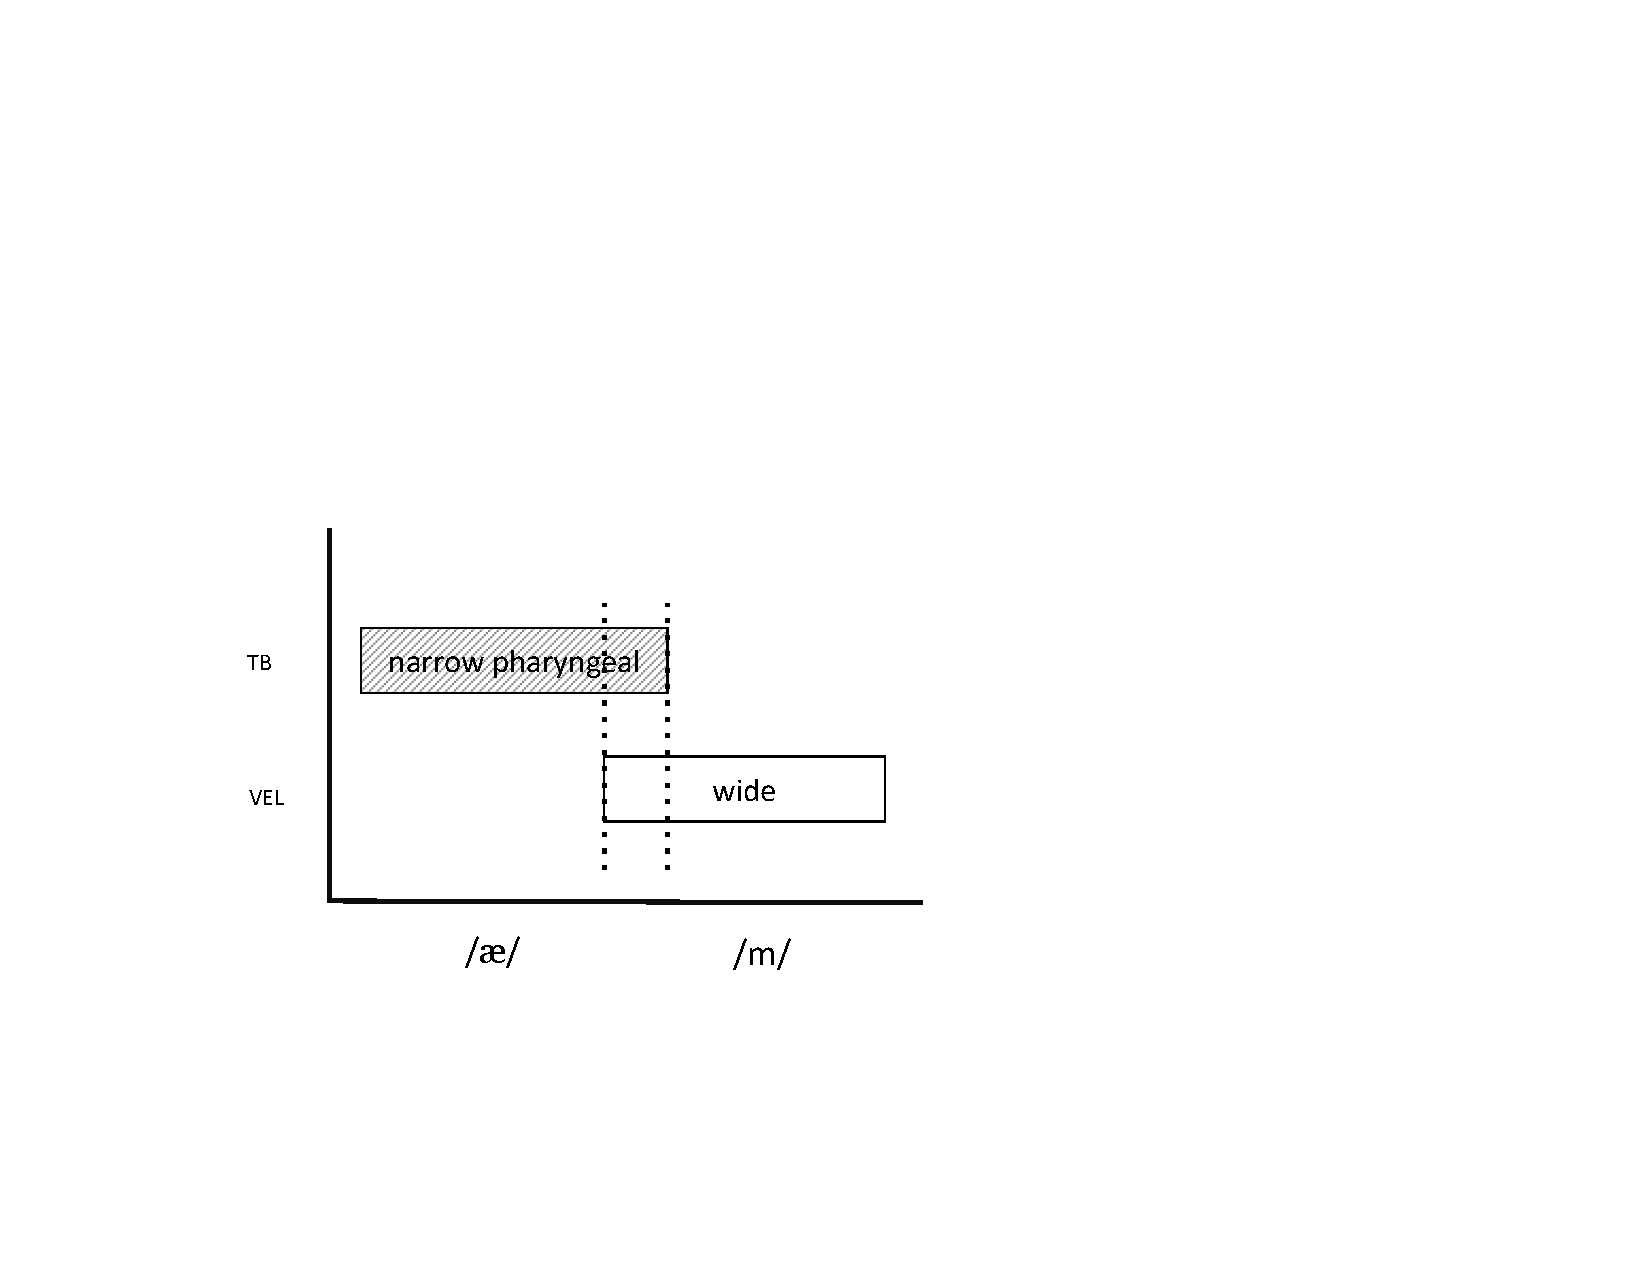
\includegraphics[width=\linewidth]{figures/nasalization1.pdf}
        \caption{\label{fig:Normal nasalization}Nasalization of underlyingly oral vowel token}
    \end{subfigure}\hfill
    \begin{subfigure}[t]{.3\textwidth}
        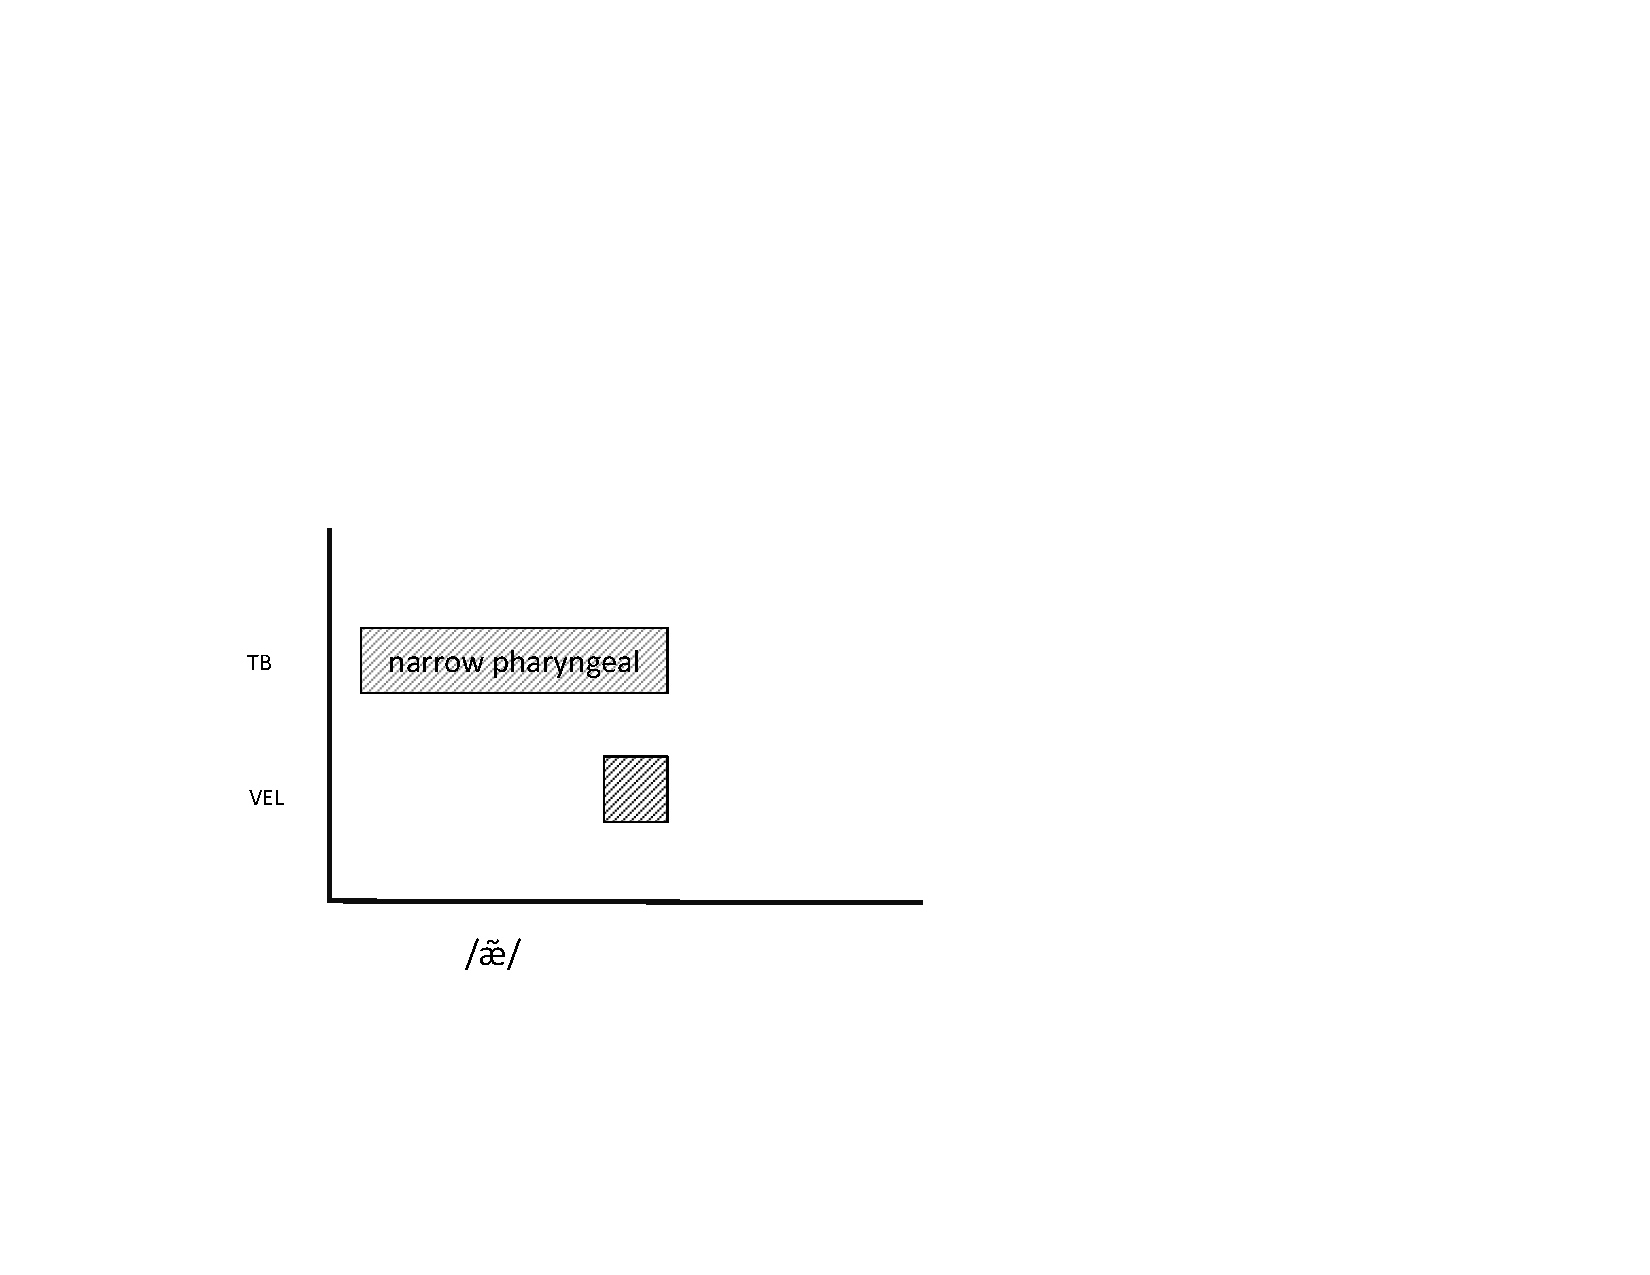
\includegraphics[width=\linewidth]{figures/nasalization2.pdf}
        \caption{\label{fig:nasalized vowel}Underlyingly nasalized vowel token (unnormalized)}
    \end{subfigure}\hfill
    \begin{subfigure}[t]{.3\textwidth}
        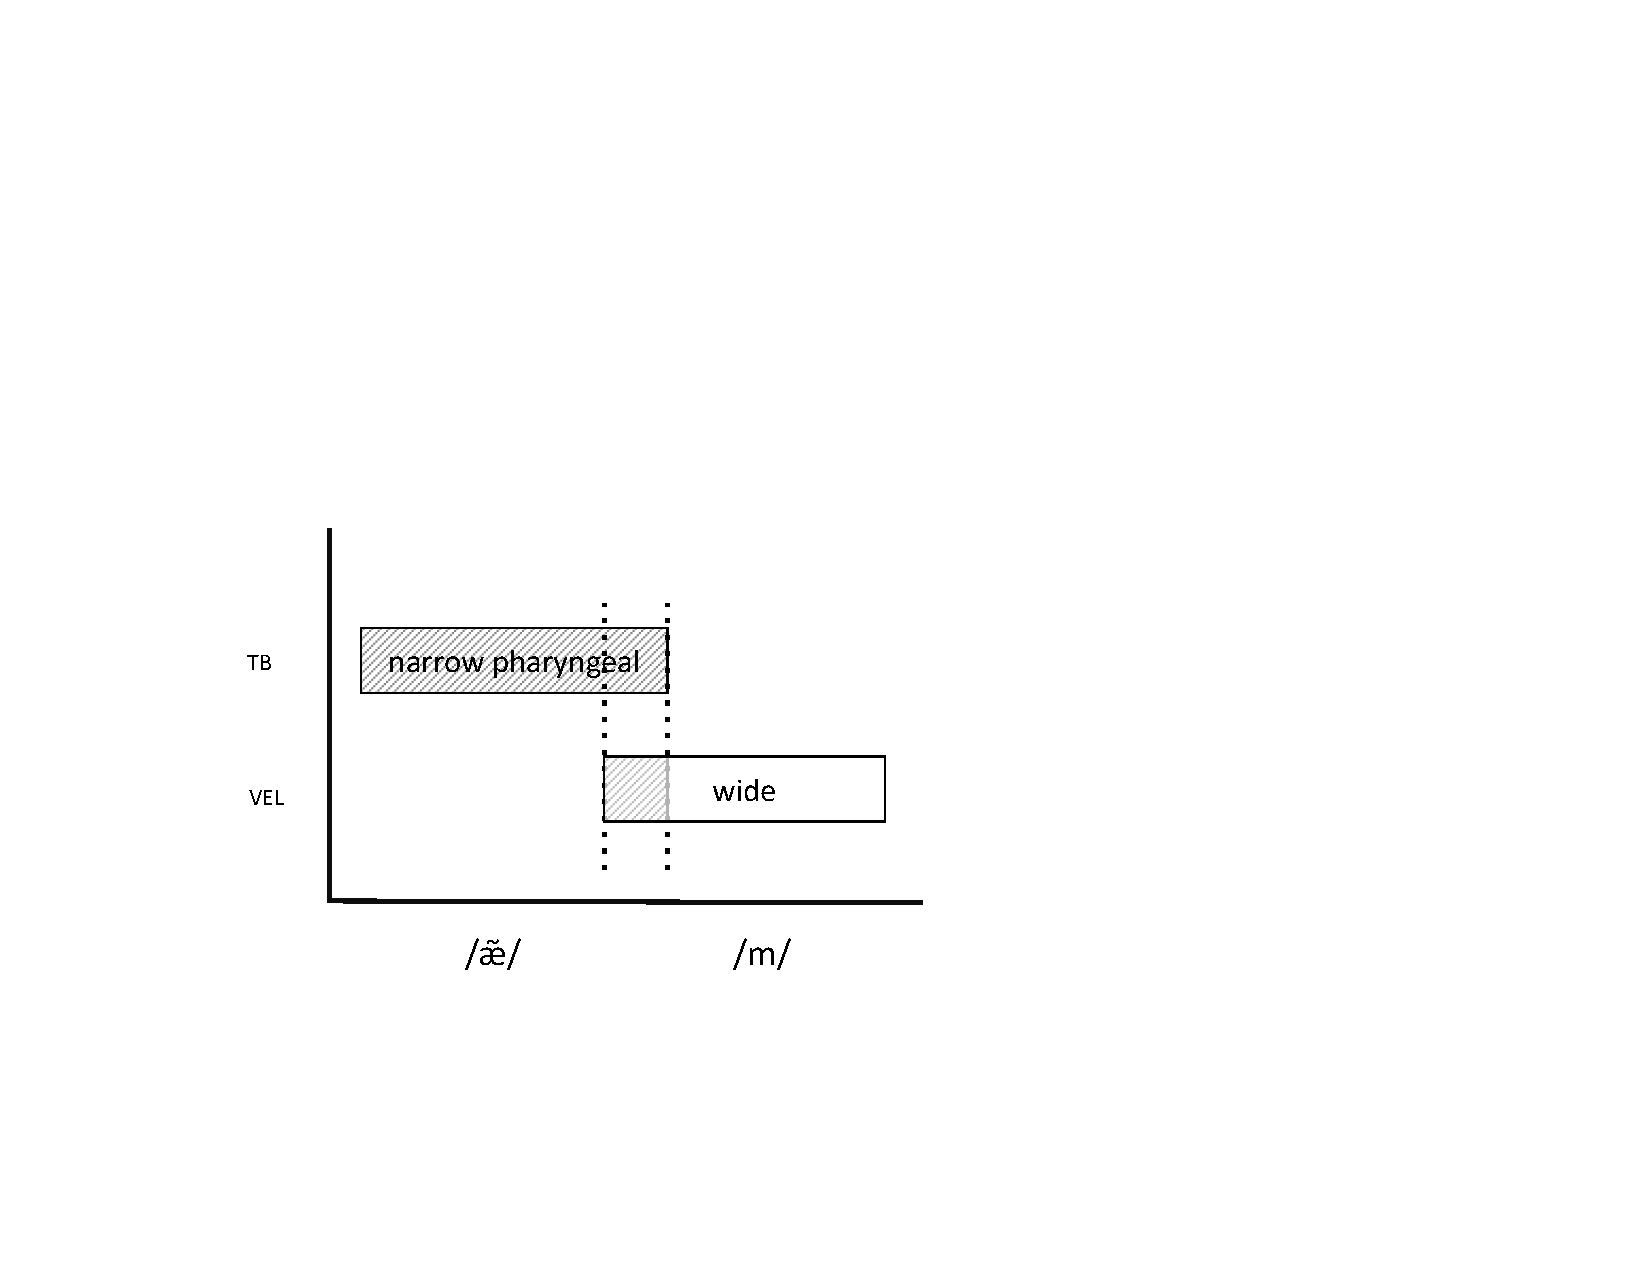
\includegraphics[width=\linewidth]{figures/nasalization3.pdf}
        \caption{\label{fig:extra nasalization}Nasalization of underlyingly nasal vowel token}
    \end{subfigure}
    
% % \subfloat[\label{fig:Normal nasalization}Nasalization of underlyingly oral
% % vowel token ]{\includegraphics[width=0.25\textwidth]{figures/nasalization̘1.pdf}}\hfill{}\subfloat[\label{fig:nasalized vowel}Underlyingly nasalized vowel token (unnormalized)]{\includegraphics[width=0.25\textwidth]{figures/nasalization̘2.pdf}}\hfill{}\subfloat[\label{fig:extra nasalization}Nasalization of underlyingly nasal
% % vowel token]{\includegraphics[width=0.25\textwidth]{figures/nasalization̘3.pdf}}

\caption{\label{fig:Coarticulation}Coarticulation involving different articulators}
\end{figure}

The gestural score indicated in \figref{fig:Normal nasalization}
produces the acoustic realization {[æ̃m]}. The vocalic
portion of this token, if stored without normalization, is represented
by {/æ̃/}. The two different types of brackets are used
here in exactly their usual sense: square brackets indicate a surface
form, an instance of speech, while forward slashes indicate an underlying
form, a form used to generate a speech act. Before such an acoustic
token can be produced, however, it must be converted to an articulatory
representation. This is shown in Fig. (\ref{fig:nasalized vowel}).
Note that, despite the fact that the nasalization is now a property
of the vowel itself, the same two articulatory gestures are still
required in production.

At some still later model cycle, when the token represented in (\ref{fig:nasalized vowel})
is chosen for production in the identical nasal context, the combined
articulatory score is realized as \figref{fig:extra nasalization}.
Under error-free perception and production, the velum gesture associated
with the vowel (indicated by diagonal fill lines), and the velum gesture
associated with the nasal will overlap completely. And because there
is only one velum, there will be only one velum gesture. Acoustically,
this will result in exactly the same amount of nasality on the vowel
as before ({[æ̃]}). The feedback loop is, in fact, halted
after a single iteration. The only way that the vowel could become
successively more nasalized is if the velum were to begin raising
earlier and earlier in time – in other words, if a successive change
in the timing relationship were to occur\footnote{Differences in the amount of velar opening and degree of velar airflow
can be found among different types of nasalized vowels (\citealt{bell1993understanding,hajek2000vowel}).
But this is a property of a given vowel. There is no reason for the
greater degree of velar opening for a low vowel, for example, to be
increased further each time that vowel is produced preceding a nasal.}. But a change of this nature requires independent motivation. In
other words, the iterative result does not come for free when the
acoustic-articulatory mapping is no longer an identity relation. 

\section{\label{sec:Competing-targets}Competing Targets for the Same Articulator}

The final case of perception-to-production mapping considered here
is one that contains conflicting consecutive specifications for a
single articulator. A common phenomenon of this type is palatalization,
which involves the tongue shifting towards the hard palate (either
forward or backward) due to the influence of a following or preceding
segment (\citealt{Guion1998,Keating1993}). Palatalization often occurs
in sequences of obstruent consonants and high vowels. For example,
in the articulation of the sequence {/ki/}, the articulatory
target of the {/k/} is the velum, or soft palate, where the
tongue body makes contact, briefly creating a complete closure in
the oral cavity. The articulatory target for the vowel is closer to
the hard palate, where the tongue body should reach its highest point,
but without making contact. As a result of the upcoming tongue body
specification for the {/i/}, the tongue position for the
{/k/} is shifted forwards – away from the soft palate, and
towards the hard palate. The result is a “blend”, something
that is in between where the two gestures would be in isolation (\citealt{Browman1986,Zsiga2000}). 

The blended production for the palatalized velar is depicted in Fig.
\ref{fig:/k+i}. At the bottom of the figure, the boxes represent
temporal extent as before, this time of the single Tongue Body articulator.
Diagonal fill lines represent the duration when the {/k/}
target is active, and the semi-opaque white, the duration of the active
{/i/} articulation. Above, the trajectory of the highest
point of the tongue body relative to the two target locations is indicated
by the dotted line. The tongue body is assumed to start from a resting
position that places its highest point somewhere in between the hard
and soft palates. With the start of the {/k/} gesture, movement
of the tongue body is initiated towards the soft palate. However,
because the gesture of the following {/i/} is anticipated,
a shift in direction takes place before this target is reached, causing
both targets to be only partially achieved (The solid curves indicate
the target trajectories for each segment in isolation). 

\begin{figure}[H]

\begin{subfigure}[t]{.45\textwidth}
        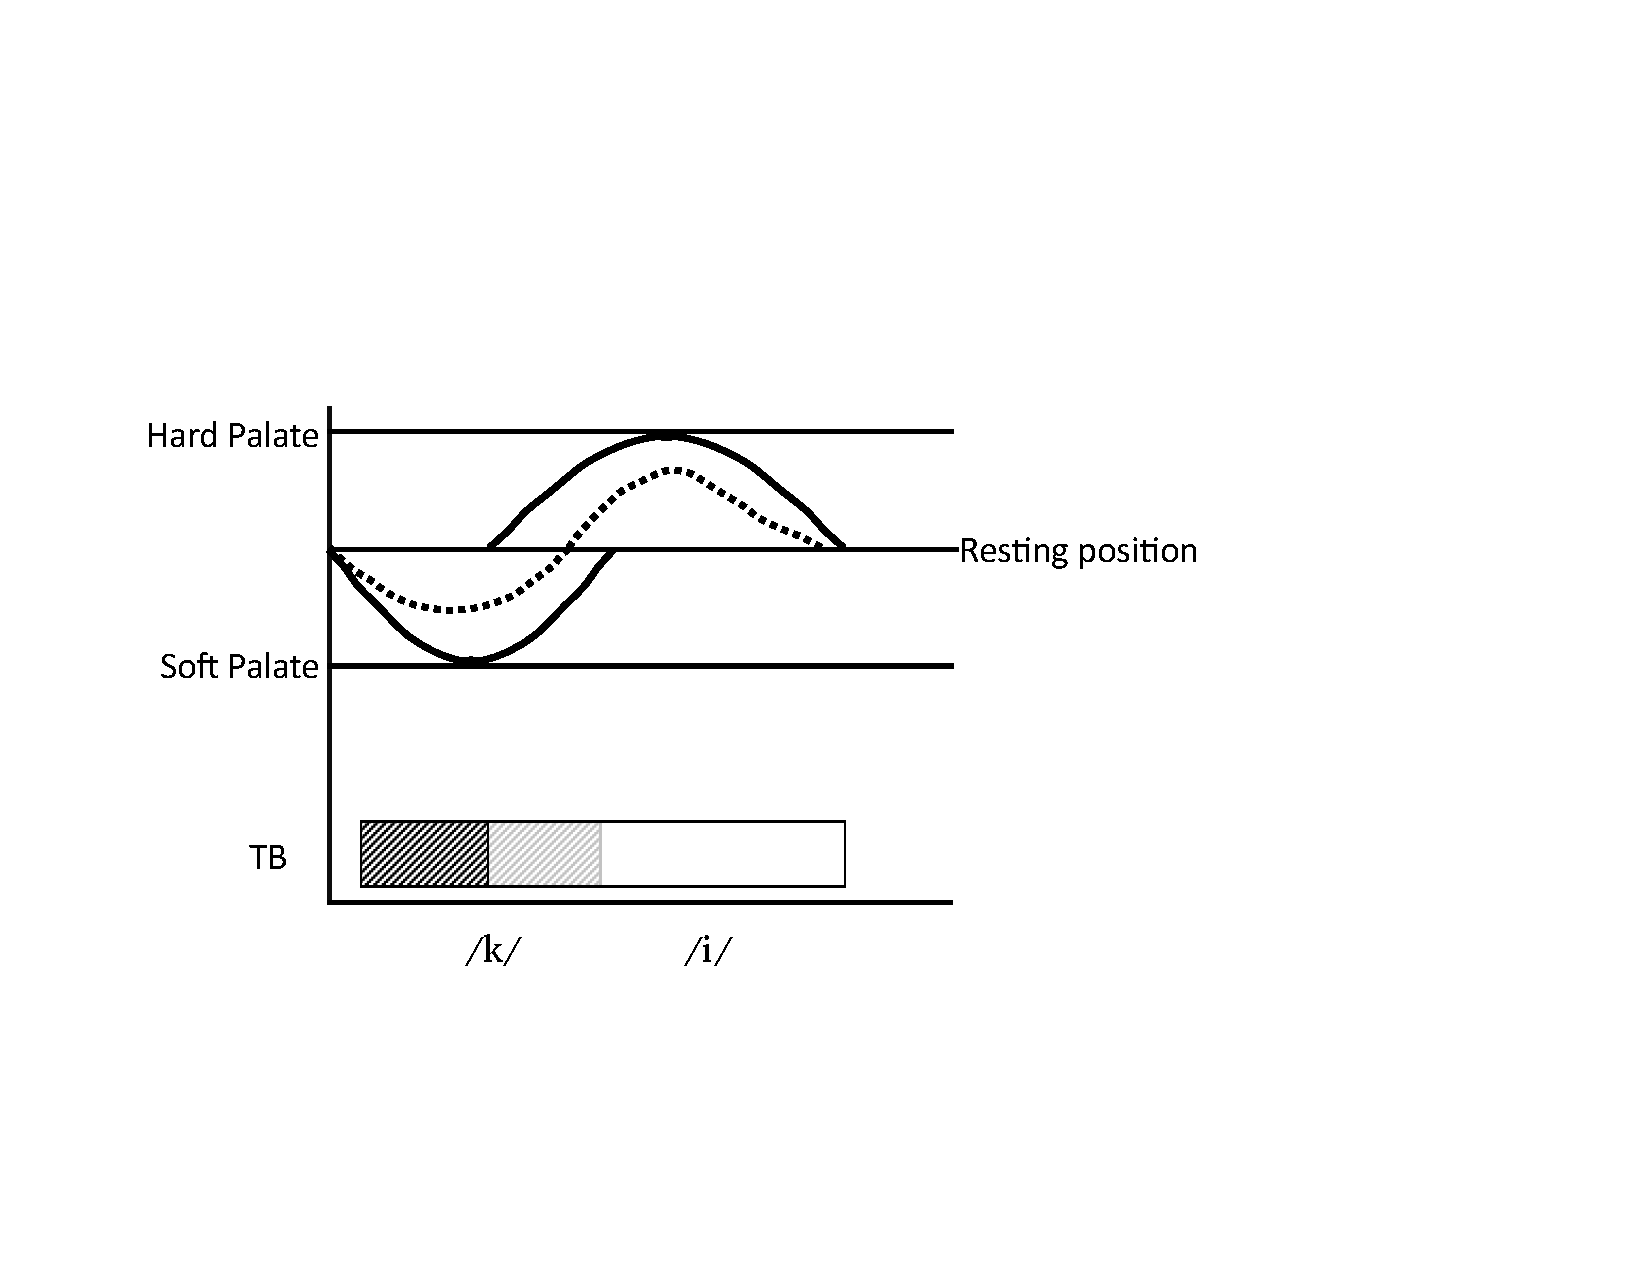
\includegraphics[width=\linewidth]{figures/palatalizationa.pdf}
        \caption{\label{fig:/k+i}/k+i/}
    \end{subfigure}\hfill
    \begin{subfigure}[t]{.45\textwidth}
        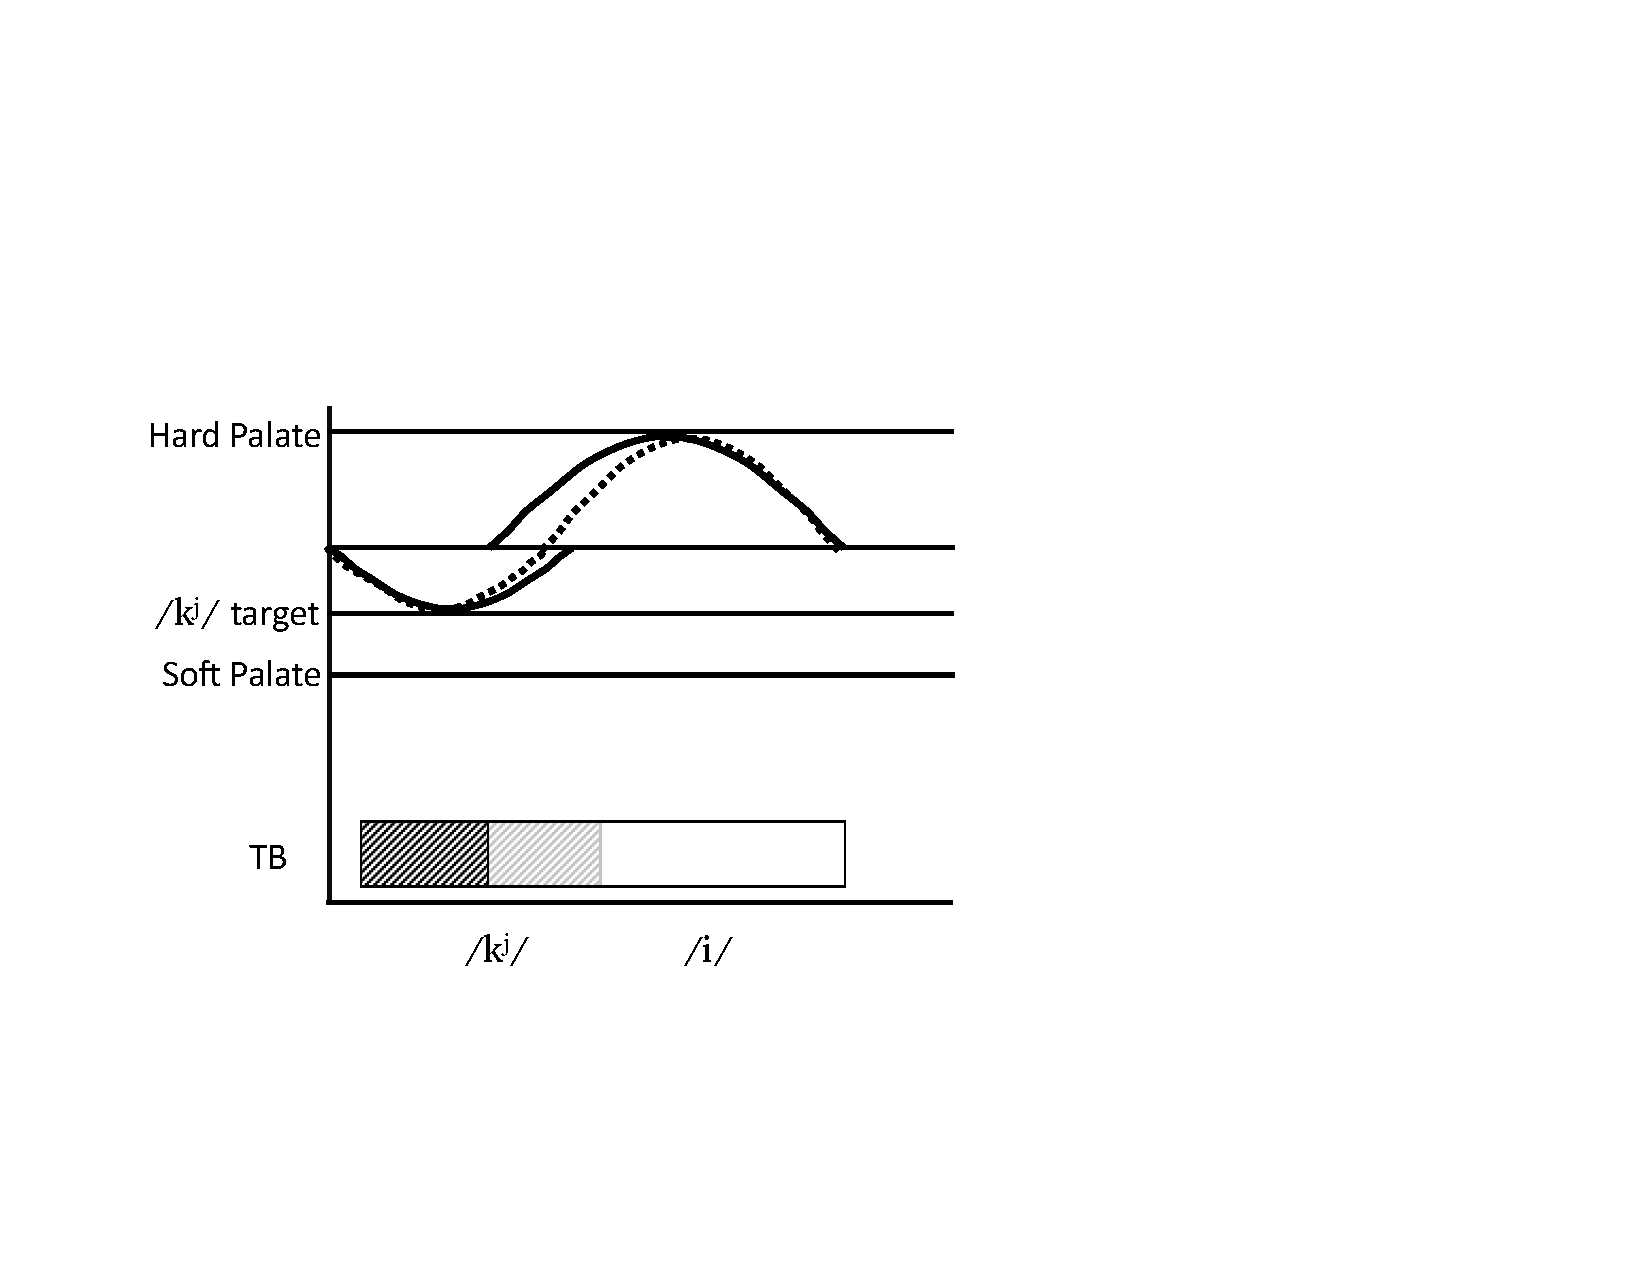
\includegraphics[width=\linewidth]{figures/palatalizationb.pdf}
        \caption{\label{fig:/k=0002B2+i/} {/kʲ+i/}}
    \end{subfigure}
    
    
% % \subfloat[\label{fig:/k+i}/k+i/]{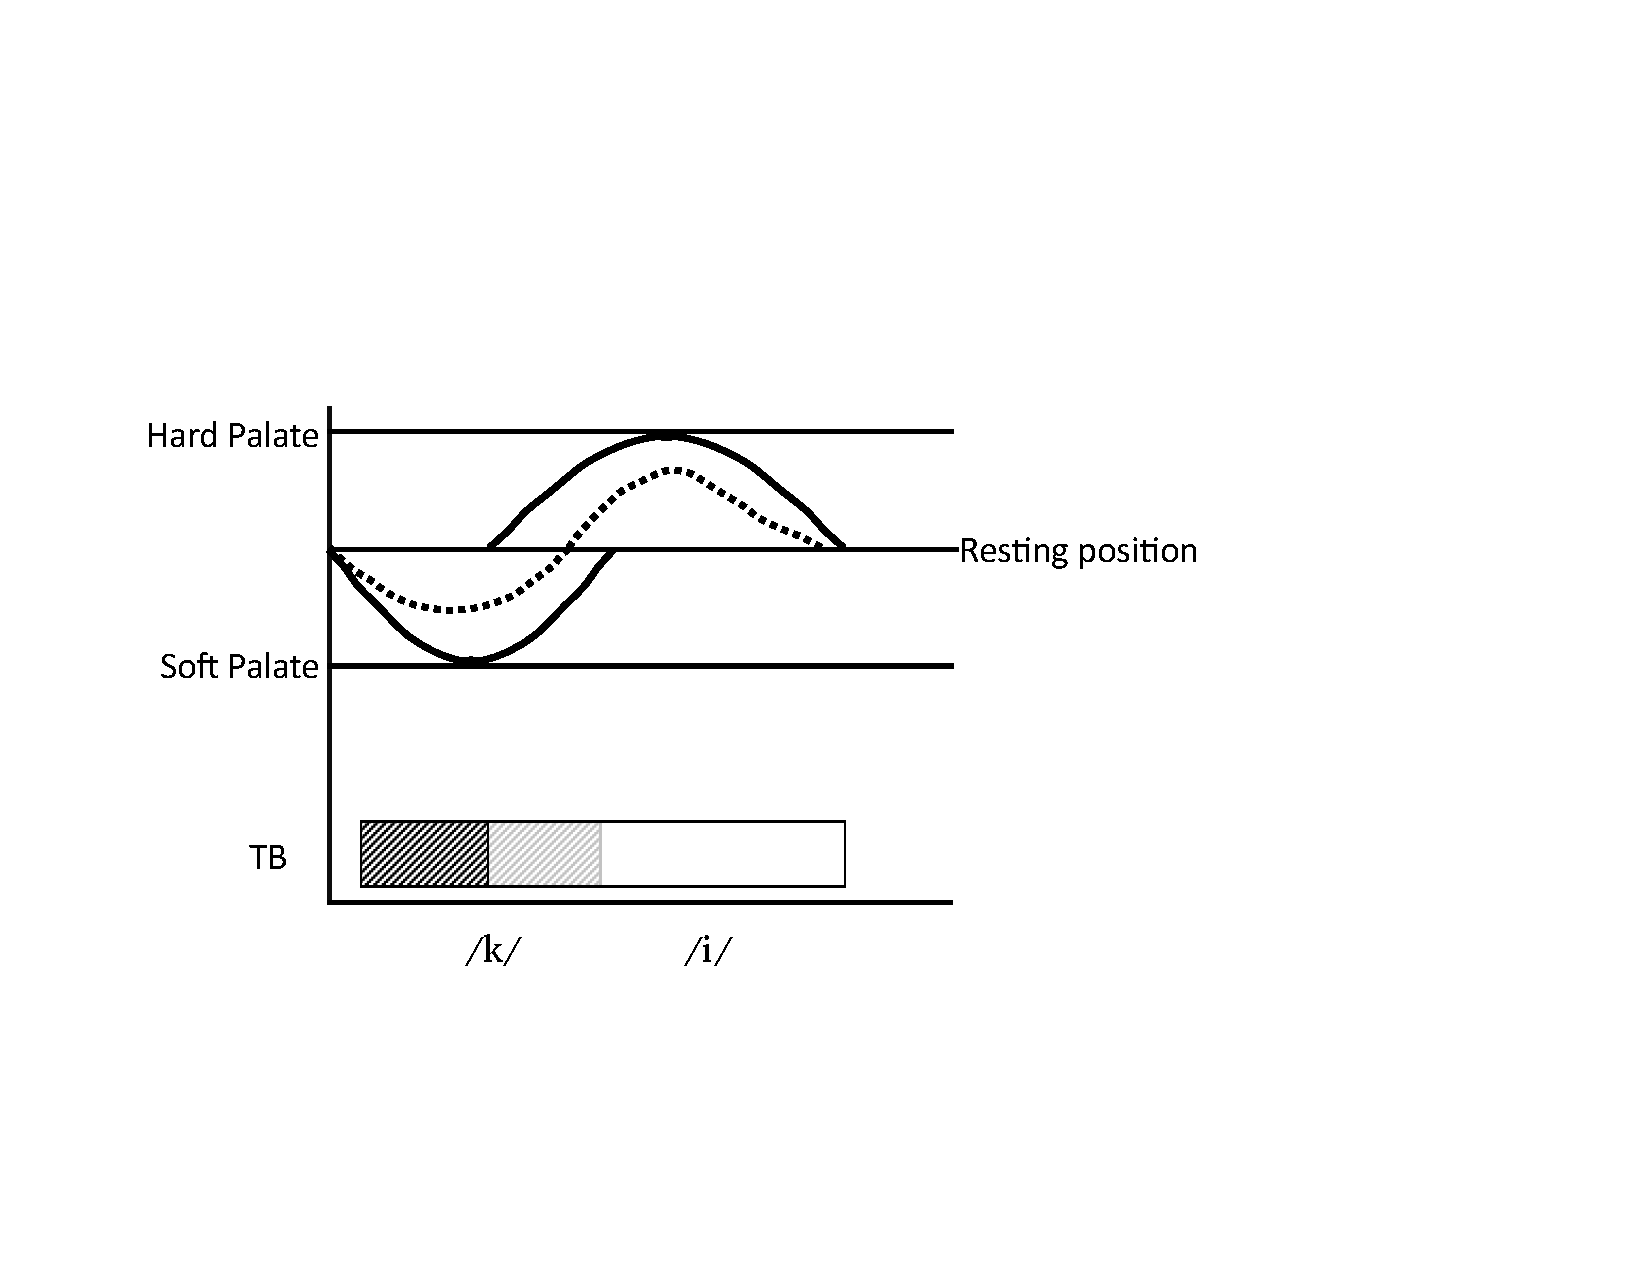
\includegraphics[width=0.4\textwidth]{figures/palatalizationa.pdf}}\hfill{}\subfloat[\label{fig:/k=0002B2+i/} {/kʲ+i/}]{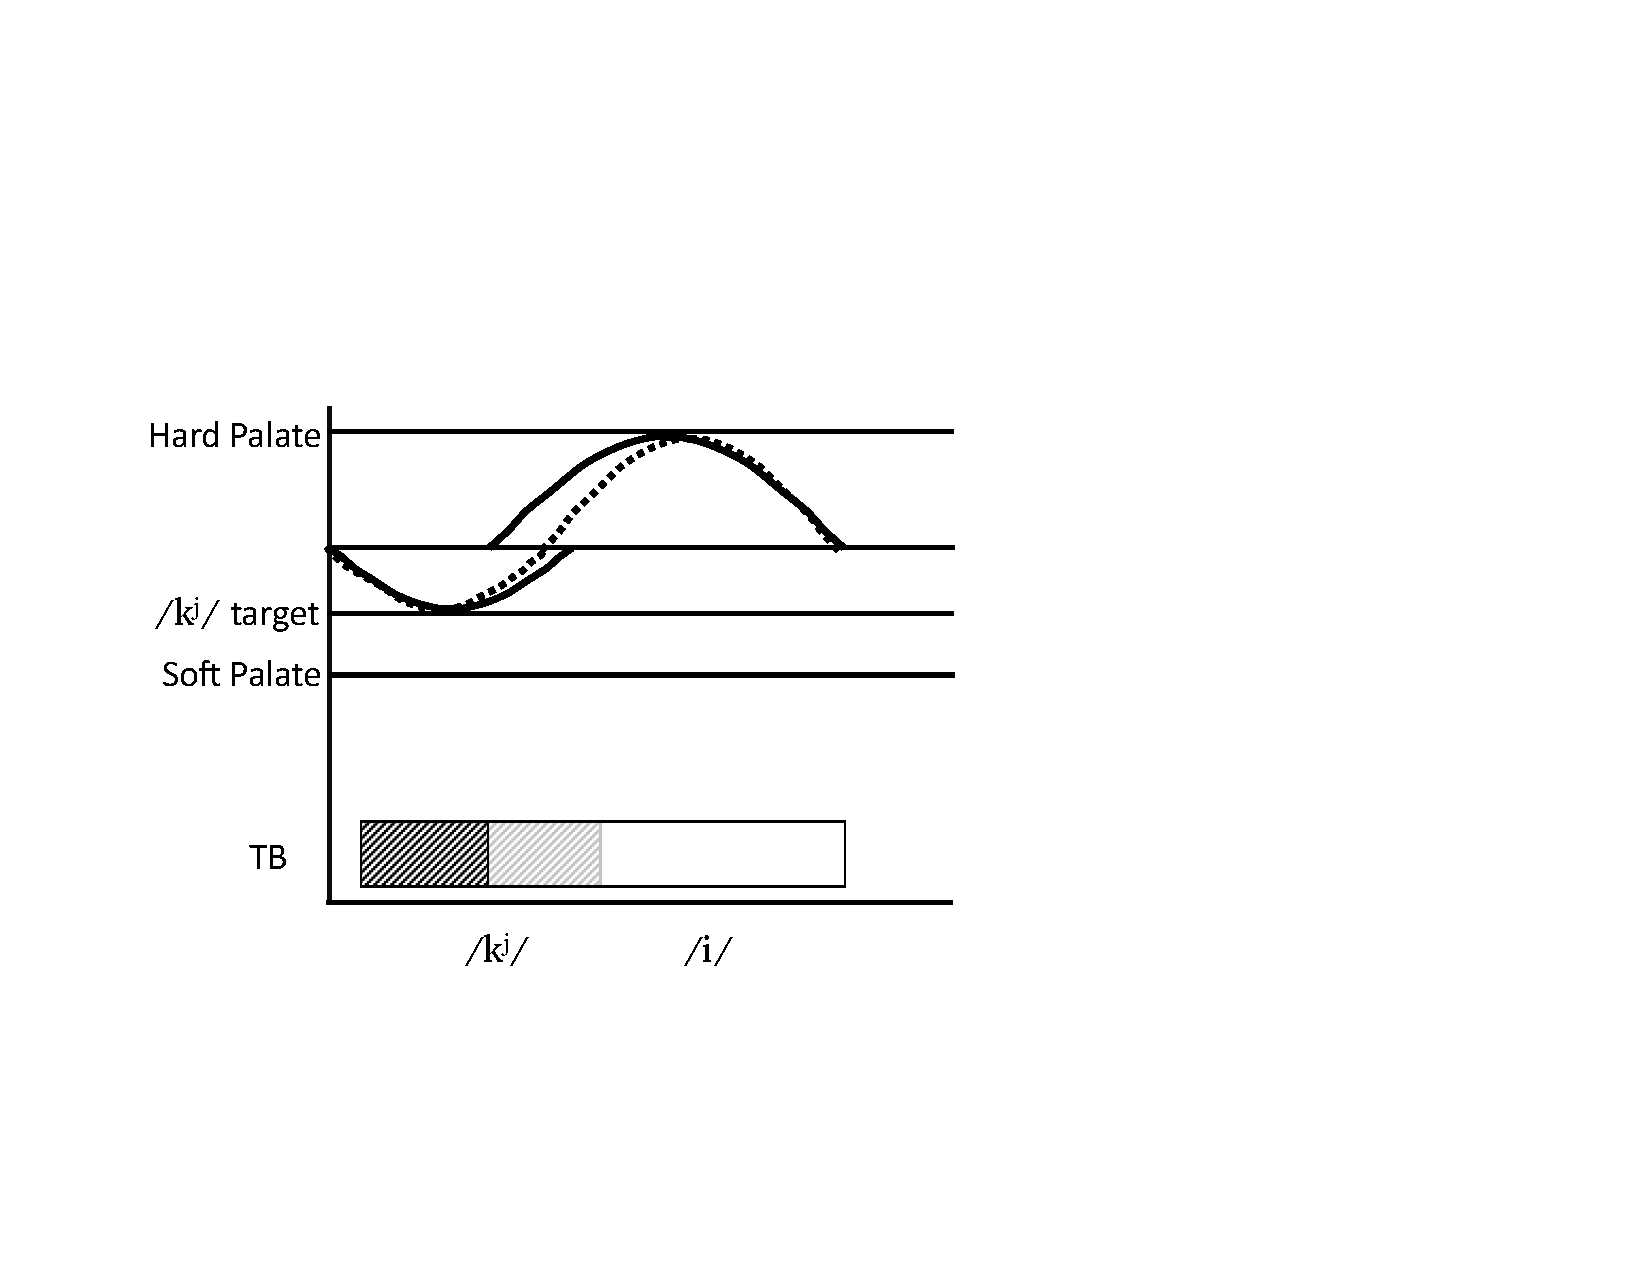
\includegraphics[width=0.4\textwidth]{figures/palatalizationb.pdf}}

\caption{Coarticulation involving the same articulator. The dark solid lines
represent the trajectories of each segment in isolation. The dotted
line represents the actual trajectory. The Tongue Body (TB) is taken
to start and finish in a resting position in between the two targets. }
\end{figure}

We will take the acoustic counterpart to this production token to
correspond to a partially palatalized k ({[kʲ]}), {[i]}
sequence. The articulatory representation associated with the acoustic
representation {/kʲ/} contains a TB gesture located at the
minimum of the dotted curve in \figref{fig:/k+i}. On a subsequent
production cycle in which this token is produced in the context of
a following {/i/} ({/kʲ+i/}), the “palatalizing
bias” will result in something like the dotted curve in \figref{fig:/k=0002B2+i/}.
Effectively, the strength of the bias has been reduced. This is because
the amount of bias depends on the distance between the two targets,
and the target of the {/kʲ/} is closer to the target of
the {/i/}. In fact, it may now be possible to reach both
targets via a slight modification in the gestural timing. In other
words, there is no clear necessity of (continuously) shifting the
target location for the obstruent closer to the hard palate, resulting
in successively more palatalized tokens. 

There is actually more than one plausible acoustic interpretation
of the output of \figref{fig:/k+i}, and thus more than one articulatory
mapping for tokens derived from the original production of the {/k+i/}
sequence. The target locations of both the consonant and the vowel
may be altered, or the perceived boundary between the two segments
may be shifted, or both. \figref{fig:Palatalizationc} depicts a
scenario in which the entire sequence has been stored as an exemplar
of the original {/k/} category: a composite segment consisting
of two sequenced targets\footnote{Using the IPA to represent acoustic correspondents is not ideal, due
not only to the conflation of acoustic and articulatory information,
but because it is not fine-grained enough to capture all the relevant
differences among the gestural scores. The composite analysis could
alternatively be represented as {/kʲ/} (as opposed to the
original {/kʲ/+/i/}). A change in both targets might look
like {/kʲ/+/ɪ/}. Other possibilities include: {/k/+/j/+/i/},
{/k/+/j/} , {/k͡j/}.}. This particular type of mapping is of considerable interest because
it is not structure-preserving at the phoneme level. If the perception
to production mapping itself might be the cause of the loss or the
gain of a phoneme, then phoneme split may be possible without an independent
change that eliminates conditioning context – may, in fact, follow
directly from a merger of the allophone with the allophonic context. 

\begin{figure}[H]
\centering{}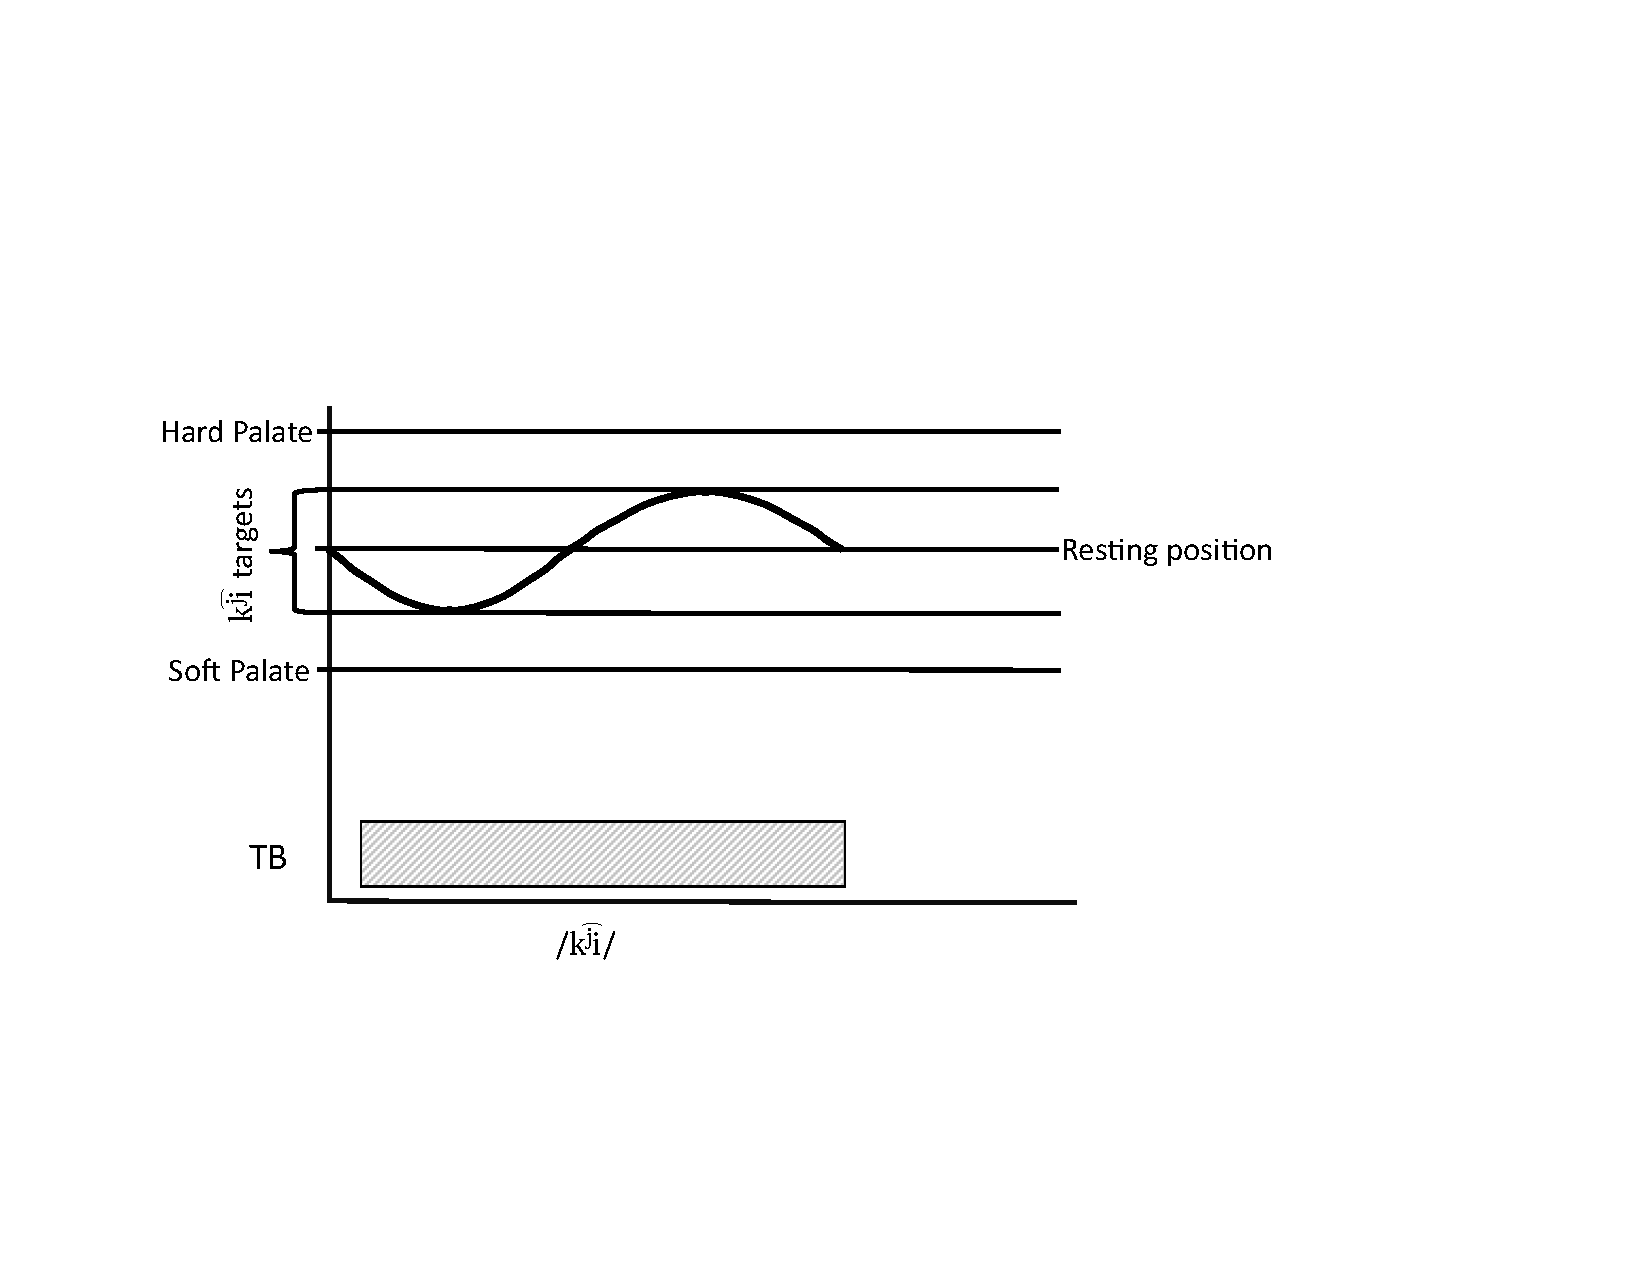
\includegraphics[width=\textwidth]{figures/palatalizationc.pdf}\caption{\label{fig:Palatalizationc}Possible production token derived from
perception token {[}{kʲi}{]}}
\end{figure}


\section{\label{subsec:Misperception-=000026-Misarticulation}Misperception
\& Misarticulation}

A well-established tradition in laboratory phonology attributes phonetic
and phonological sound change to mishearing and misspeaking on the
part of individual speakers and listeners (\citet{Ohala1980,Ohala1981,ohala1983origin,Ohala1990}).
Many such changes are traced to coarticulation in production, which
can create perceptual ambiguity, and the possibility that what the
listener recovers is not what the speaker intended. In certain theories
of change, the rarity of sound change is attributed to the fact that
most speech takes place in a mode where speakers provide sufficient
cues for listeners, and listeners accurately reverse the effects of
coarticulation. Only rarely do listeners switch to a `non-speech'
mode, in which they take the perceived forms at face value, or randomly
decide to keep a poor category exemplar, rather than discard it (e.g.,
\citealp{lindblom1990explaining,Garrett2013}). In other theories,
discrepancies between speaker and listener are more common, and the
rarity of language-wide change is attributed to the listener's access
to other sources of information about the `correct' form of a word
(and/or the low likelihood of other speakers adopting and spreading
an individual's novel variant (e.g., \citealt{Ohala1980})). 

Perception biases emerge when segment \emph{x} is more likely to be
misheard as segment \emph{y}, than segment \emph{y} to be misheard
as segment \emph{x}. Production biases, in some cases, can be attributed
to the masking of overlapping articulatory gestures in rapid or casual
speech. These biases are of the same kind as those adopted in the
preceding models. Yet a fundamental aspect of the nature of these
misanalyses has been lost in implementation. Even in models that explicitly
invoke the Evolutionary Phonology framework (see \citealt{Blevins2004}),
the mechanism is typically realized at a very coarse grain\footnote{Although \citet{Boer2000} uses a non-trivial mapping from acoustic
data to production targets, it is not a model of sound change, but
of structure emergence in vowel systems. In a similar type of model,
\citet{oudeyer2006self} relies on the same units (neurons) being
used in perception and production. However, this mapping is mediated
by the distributed nature of the representations (over a network of
neurons), and the fact that neurons are `tuned' by experienced input,
via a non-linear activation function. }. For example, the model in \citet{wedel2017category} (also described
in \citet{Blevins2009}) is driven by misperception error (or “variant
trading”); this occurs as a binary decision between neighboring
lexical categories. As already discussed, \citet{Garrett2013} implement
an all-or-nothing normalization mechanism\footnote{Although they make an explicit distinction between a word-level perceptual
token space, and a segment-level production token space, no transformation
algorithm is provided. They also suggest that the articulatory `speech'
mode is sometimes available for perception, so the exact relationship
between the two `modes' of processing is somewhat unclear. In practice,
the models seem to be implemented using a single abstract phonetic
dimension.}. In \citet{Kirby2014}, `misparsing' is more gradient; for any given
token, a random amount of the target segment may be mis-attributed
to the preceding segment. However, the misparsing doesn't depend on
the phonetic properties of the input, and different outcomes are only
possible by `turning off' the misparsing. \citet{morley2014implications}
uses a bi-directional misperception term in a model of velar palatalization,
but misperception only applies to feature parsing, and is segment
preserving. 

In the next chapter a new model of vowel nasalization is developed,
guided by the goal of avoiding the theoretical and implementational
pitfalls laid out in this, and preceding, chapters. This model will
contain an explicit perception-to-production analysis stage in which 

\chapter{Phoneme split}\label{ch:Phoneme-Split}

In this chapter we will develop a model of phoneme split, or genesis,
using the phenomenon of vowel nasalization as a case study. The model
will be based on the analyses of the preceding chapters: the metric
of success will be representational consistency and stability, with
the ability to achieve multiple stable states under different parameter
settings. The relevant parameters will also be required to serve as
testable hypotheses about possible actuation mechanisms. The first
of two model variants, the No-Phoneme Model, will contain explicit
representations only at the word level, and will be used primarily
to illustrate a particular implementation of the frequency effect.
The subsequent model, the Multiple-Parse Model, will add a sub-lexical
level of analysis. The major innovation of this model will be an explicit,
non-one-to-one, perception-to-production mapping in which the likelihood
of a given analysis depends on the phonetic properties of the input.
Additionally, no analysis is taken to be more ``correct'' than any other,
just as the set of possible sub-lexical units is not taken to be determined
ahead of time.

\section{Representations I}

It has been well-established in both perception and production that
there is a negative correlation between degree of vowel nasalization and strength
of nasal consonant (e.g. \citealt{kawasaki1978perceived,cohn1990phonetic}).
This is consistent with the hypothesis that the final nasal is more
likely to be lost, the more nasalized the preceding vowel becomes.
A possible explanation can be found in a listener-oriented theory
of change, where speakers strive to preserve acoustic cues for ease
of listener comprehension. Strong nasal cues on the vowel predict
the upcoming nasal, which means that speakers may expend less effort
to preserve the actual nasal, allowing it to erode. As with other
proposals, the question that still remains to be answered is how the
vowel came to have such strong nasal cues in the first place (presumably
stronger than the typical range of phonetic nasalization observed
cross-linguistically). 

A different perspective will be adopted here, building on the observation
of \citet{Beddor2009} that the negative correlation between vowel
nasality and consonant nasality follows directly from a single articulatory
parameter: the degree of overlap of the vowel and nasal gestures.
The more overlap, the greater the extent of nasalization on the vowel,
and the shorter the duration of the purely consonantal nasal, and
vice versa (see \figref{fig:Normal nasalization}). It will be assumed
that successful production requires stored articulatory targets, and
that these must be inferred from acoustic inputs. For simplicity,
only a single word type will be modeled, that consisting of a tongue
body gesture followed by a velum gesture (e.g. “am”). The production-perception
mapping will take place over three phonetic variables: duration of
tongue body gesture, duration of velum gesture, and duration of gestural
overlap $(x^{V},x^{N},x^{O})$. Categorization will occur at the level
of the word, and does not require decomposition into phonemes. Thus,
these models will not assume that there exists an allophonic process
of vowel nasalization. The initial distributions for all tokens will
be generated by independent sampling from three separate normal distributions,
corresponding to $x^{V}$, $x^{N}$, and $x^{O}$, respectively. 

In \chapref{ch:Models-of-Change} we saw that (soft) targets
were needed to constrain the basic exemplar model of change. What
this did was effectively force an independent production component
into a model which otherwise equated acoustic and articulatory representations.
In the current set of models this is not necessary, implementationally,
or conceptually, because each acoustic token has its own production
target. This is depicted schematically in \figref{fig:P-toP-mapping},
where stored articulatory parameters (represented by temporally overlapping
articulatory gestures) are realized as acoustic tokens during production
(dark patterned rectangles representing sound frequency information
over time), and acoustic tokens are, in their turn, transformed into
stored articulatory parameters during perception. At the word level,
this is a \noun{state} model; the articulatory variables are stored
without normalization. At the gestural level, however, there is the
possibility of an implicit \noun{process} model in the fact that the
overlap dimension represents the concatenation of two units, as well
as the source of nasalization. We will return to this point below.

\begin{figure}[H]

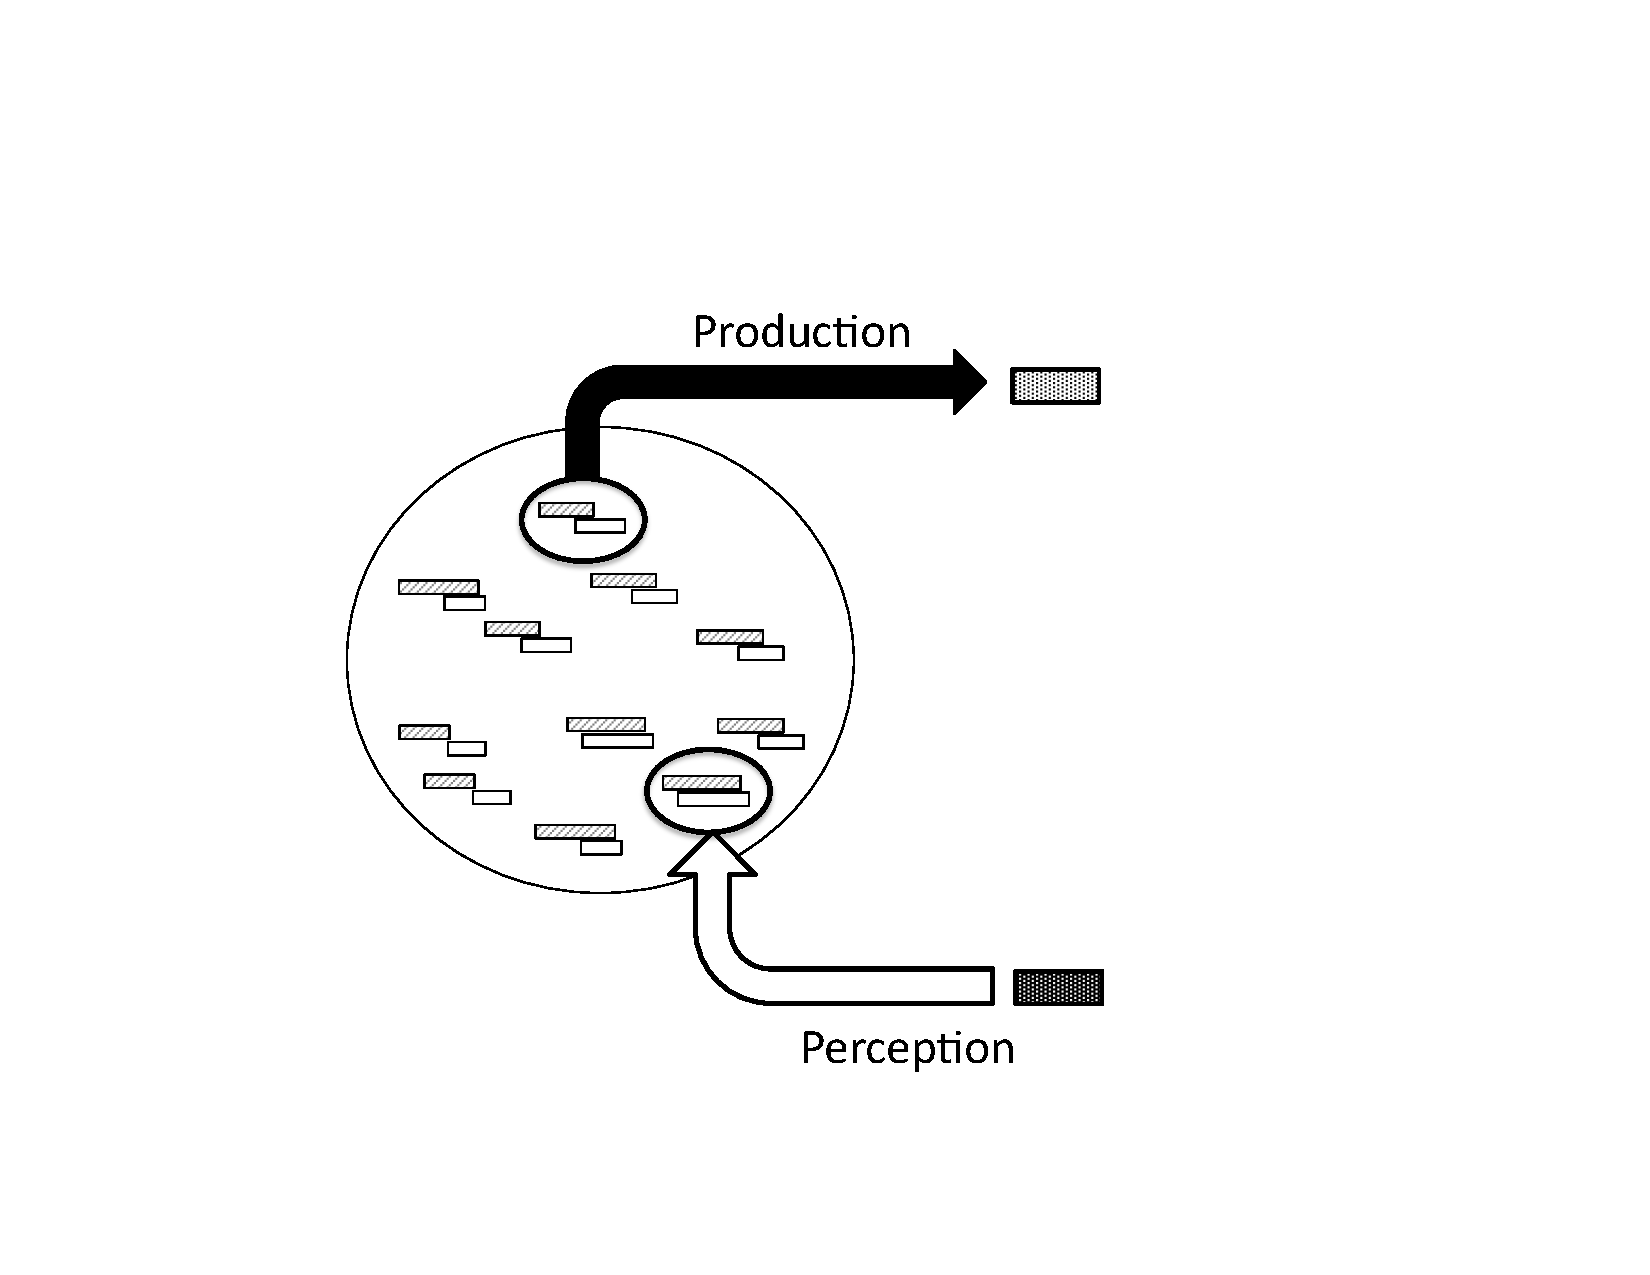
\includegraphics[width=0.45\textwidth]{figures/SeparateReps.pdf}\caption{\label{fig:P-toP-mapping}Graphical depiction of an explicit mapping
between articulatory representations and acoustic representations }

\end{figure}

As \sectref{sec:Model-Behavior} showed, the two-attractor (\noun{state}
model) had a limited range of output states: the entire distribution
always stabilizes at some point intermediate between the two attractors.
Furthermore, that model contained no mechanism for changing the attractor
locations, or introducing new attractors. The current model effectively
explodes the number of attractors (or underlying representations)
to the number of tokens within a category. This allows for more complex
model dynamics. It also allows for changes to occur to the attractors
themselves, via independent forces that act, not at the level of the
word (or at the level of the phoneme), but at the level of the gestural
variables. Individual tokens of a given word category can thus be
altered, with the possibility, but not the guarantee, that such changes
can spread throughout the entire distribution of tokens.

\section{\label{sec:Frequency-I}Frequency I}

The first iteration of the phoneme-split model uses a frequency-based
attractor as the actuator of change. Based on the assumption that
frequency-based reduction is the result of increased fluency, and
that to be fluent is to produce some (nearly) ideal balance of efficiency
and intelligibility, an optimal degree of gestural overlap, \emph{T},
is defined. Relative word frequency is implemented as a parameter
($\beta$; $0<\beta<1$) that controls the degree to which each token
of the category is shifted towards the target, \emph{T}, during production.
Thus, for a stored production token consisting of the duration triple
$(x_{i}^{V},x_{i}^{N},x_{i}^{O})$, a fluency effect applies to the
ultimate realization of $x_{i}^{O}$, the gestural overlap value,
in the following way: 
\begin{equation}
\textit{Fluency}:x_{i}^{O^{\prime}}=x_{i}^{O}+\beta(T-x_{i}^{O})\label{eq:Frequency attractor}
\end{equation}
Because the absolute duration of the optimal gestural overlap will
depend on the durations of the gestures for each specific token, $T$
is expressed as a function of $x_{i}^{N}$. In the case where $T=x_{i}^{N}$,
the fluency pressure always acts to increase $x_{i}^{O}$ (as long
as $x_{i}^{O}\neq x_{i}^{N}$), because the duration of overlap can
never be larger than the duration of the nasal gesture (assuming also
that $x_{i}^{V}$ is always greater than $x_{i}^{N}$). 

\section{Speaking rate}

As has already been demonstrated several times, a single attractor
results in a single possible outcome. With only the frequency attractor
acting on productions, maximal fluency is the only possible outcome,
regardless of the value of $\beta$. Implementationally, a force is
needed to counter-act the fluency effect. For a fluency target at
maximal overlap, that opposing force must act to decrease overlap.
However, in the general case, it may be desirable to include a force
that can either increase or decrease the relevant parameter values.
In fact, regardless of the implementational requirements for a successful
model, there are clear theoretical reasons to include a bi-directional
force affecting articulatory durations. 

Changes in speaking rate, of course, strongly influence the absolute
duration of speech sounds. Furthermore, there are similarities between
the reduction effects observed in fast speech, and those observed
with high-frequency words. Therefore, whatever drives changes in speaking
rate is clearly relevant in a model of change in which duration plays
a role. Equally important is the fact that changes in speaking rate
are not all increases in speed, and the effect of slowed speech in
potentially disrupting cumulative change cannot be selectively ignored. 

Changes in speaking rate have been shown to affect both the absolute
duration as well as the timing between sequential speech units (\citealt{stetson1928motor,Hardcastle1985}),
and therefore are taken to affect all of $(x^{V},x^{N},x^{O})$ in
the phoneme-split model. I will adopt the view here that changes in
speaking rate are governed by forces largely external to the mechanisms
of sound change, and that changes in rate can therefore be modeled
as a stochastic process.\footnote{There is a strand of research that assumes that changes in speaking
rate, specifically decreases in speaking rate, are driven by a desire
to enhance or exaggerate a given phonological contrast (e.g. \citealt{beckman2011rate}).
Although slowed speaking rate often occurs under conditions in which
speakers are deliberately hyper-articulating their speech, I assume
that decreases in speaking rate can also occur independently; that
is, that speakers can control their rate of speech, e.g. when asked
to match the beat of a metronome, without consciously trying to produce
more intelligible speech.}

Changes in speaking rate, affecting word duration, are modeled in
the following way. At production, a value is randomly selected from
a normal distribution centered about 0. This value represents the
force (\emph{E}) that will act on that token: either to expand it
(if positive), or to compress it (if negative). Expansion results
in longer words, corresponding to slower speaking rates, and compression
results in shorter words, corresponding to faster speaking rates.
Each articulatory parameter is independently subjected to this force.
The degree to which a given gesture is actually expanded or compressed
depends on how inherently elastic it is. This elasticity is implemented
as a parameter that controls the steepness of a logistic curve. For
example, the effect of force \emph{E} acting on the overlap variable
($x^{O}$) is given in Equation (\ref{eq:Speaking rate transform}): 
\begin{equation}
\textit{SpeakingRate}:x_{i}^{O^{\prime\prime}}=\frac{A}{(1+e^{kE})}\label{eq:Speaking rate transform}
\end{equation}
\emph{A} is a normalization factor, and is set to $2x_{i}^{Z^{\prime}}$
for all variables (\emph{Z}). This has the effect of making the adjusted
length depend on the current length, with $E=0$ resulting in no change.
Note that for decreases in speaking rate, overlap should decrease
– pulling the two gestures apart, and thus lengthening the word –, while for increases in speaking rate, overlap should increase. Therefore,
the dependence of overlap on expansion degree is expressed as a positive
exponential, while the dependence of the other two duration parameters
is expressed as a negative exponential. For these simulations all
three articulatory variables were set to the same elasticity ($k=1$). 

\section{\label{sec:No-Phoneme-Phoneme-Split-Model}No-Phoneme Phoneme-Split Model}

In order to understand the behavior of the phoneme-split models, we
first create a version with only the speaking rate mechanism included.
Figure \ref{fig:SpeakingRateOnly} shows the outcome that the speaking
rate distribution (\emph{E} distribution) selects for, given a particular
starting distribution of tokens. The three articulatory parameters
are plotted separately, in different colors. This model also assumes
error-free mapping of acoustics to articulation, outside of a small
error term in production. Entrenchment and memory decay apply as in
previous models.

\begin{figure}[h]
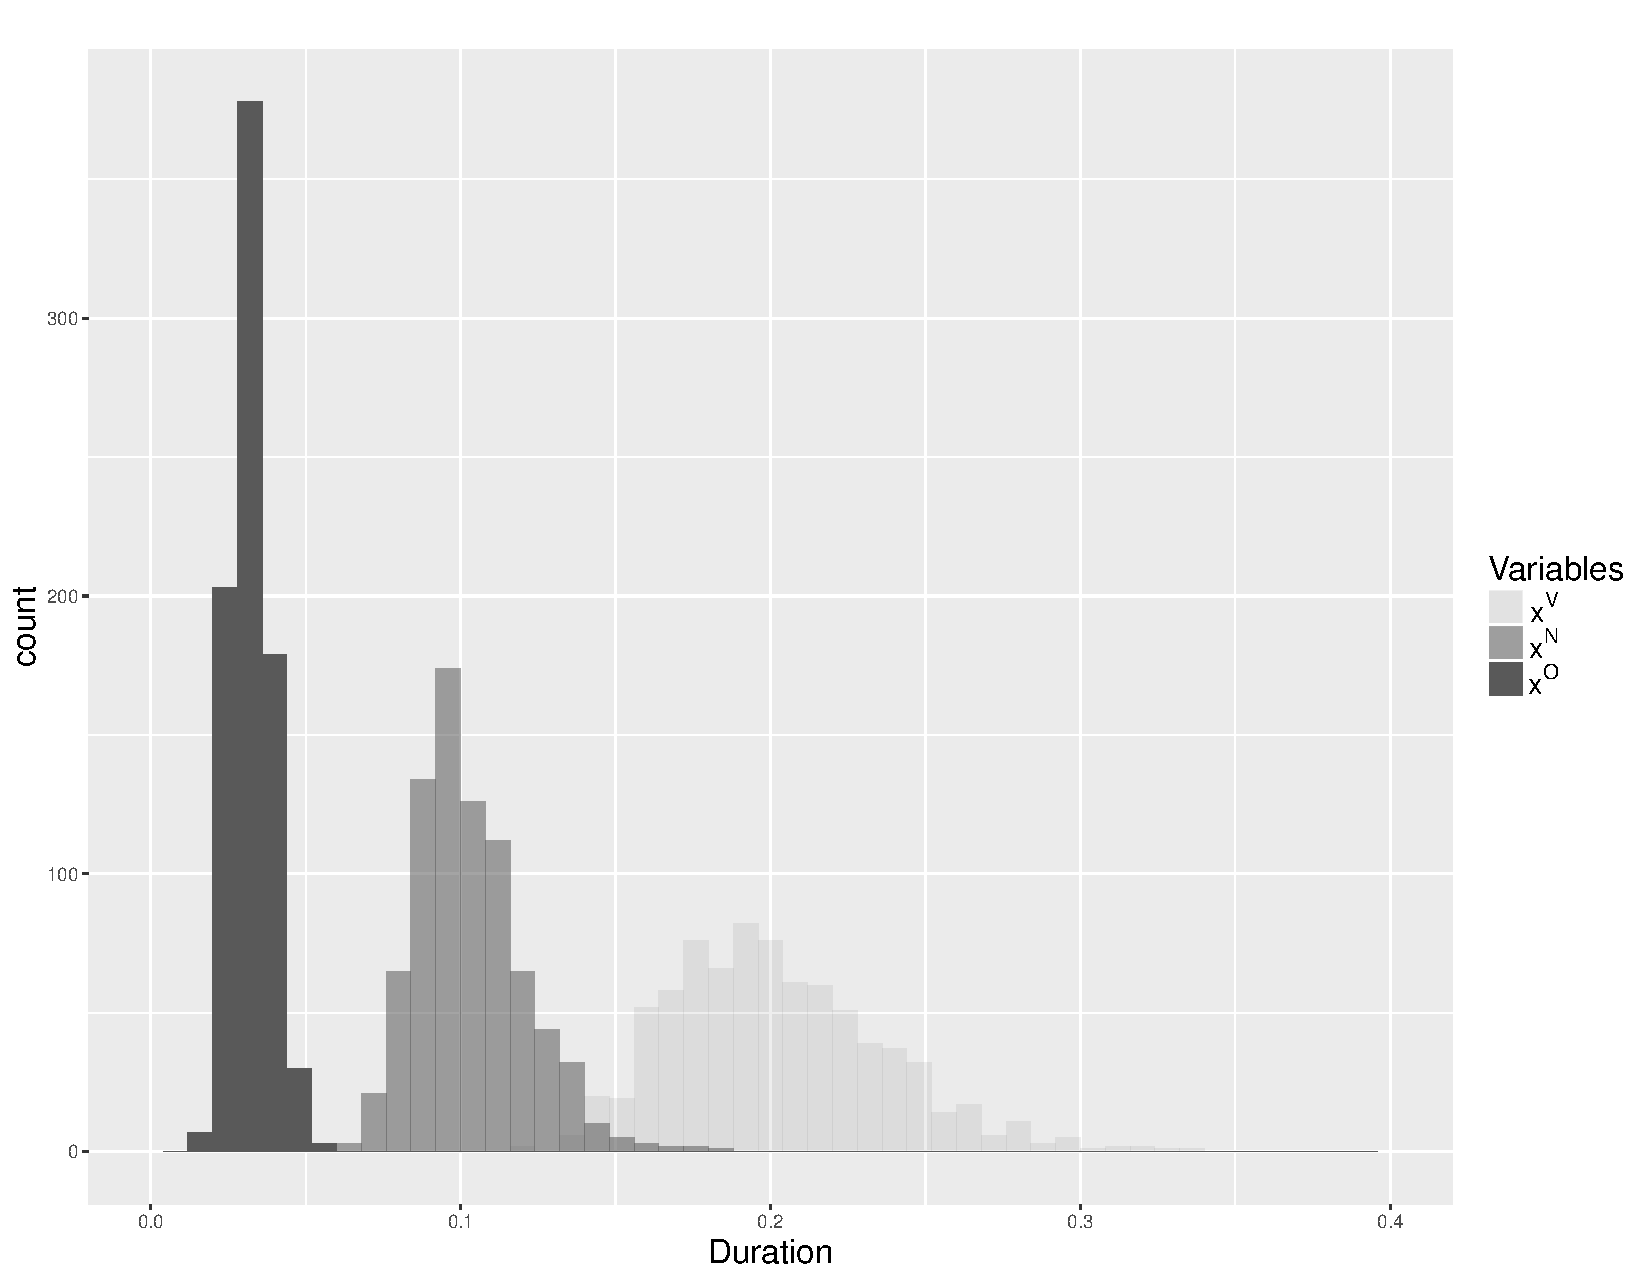
\includegraphics[width=0.6\textwidth]{figures/SpeakingRateI10000.pdf}\caption{\label{fig:SpeakingRateOnly}Phoneme-Split Model: Speaking rate only}
\end{figure}

With appropriately chosen constants, the speaking rate force is capable
of disrupting the influence of the frequency-based attractor. This
allows the equilibrium state of the model to vary as a function of
word frequency ($\beta$). For $T=x_{i}^{N}$, the fluency effect
acts consistently to increase gestural overlap ($T=x_{i}^{N}$). If
it is too weak ($\beta$ too small), then the speaking rate equilibrium
shown in Figure \ref{fig:SpeakingRateOnly} prevails. If it is strong
enough, then it is able to shift the overlap distribution to larger
values (rightward). This is possible because the speaking rate transform
depends on the current value of the overlap parameter for any given
token (expressed in the variable \emph{A} of Eq. \ref{eq:Speaking rate transform}).
Figure \ref{fig:NasalizationModel1} shows the output of the model
with both speaking rate and frequency bias, run for three different
values of $\beta$. Note that the number of model iterations is essentially
arbitrary. Because the number is large (10,000), there is a reasonable
expectation that a stable state has been reached, but no tests of
convergence were performed. In this section we are more concerned
with the qualitative behavior of the model, and comparisons in which
all but one aspect of the simulations are kept constant.

\begin{figure}[h]

\begin{subfigure}[t]{.3\textwidth}
        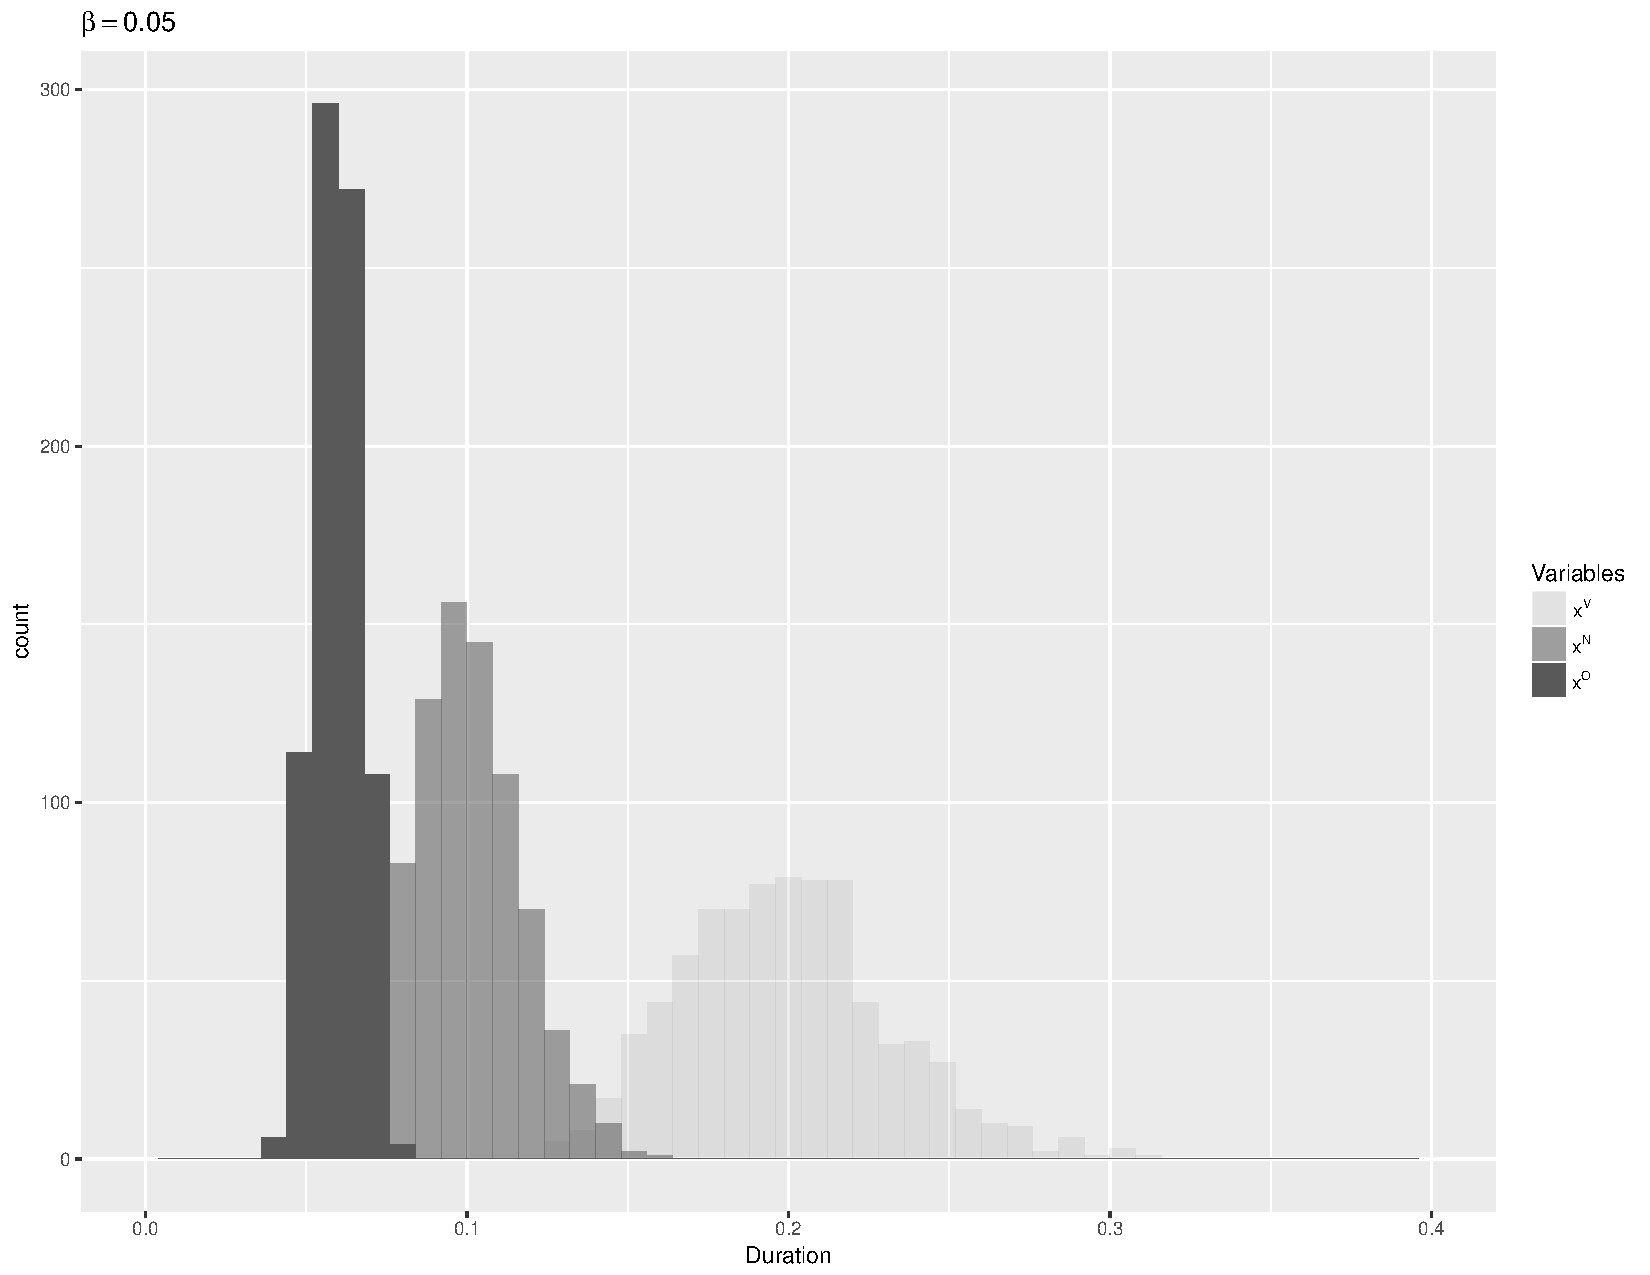
\includegraphics[width=\linewidth]{figures/SpeakingRateFrequencybeta05.pdf}
        \caption{Low-frequency word ($\beta=.05$)}
    \end{subfigure}\hfill
    \begin{subfigure}[t]{.3\textwidth}
        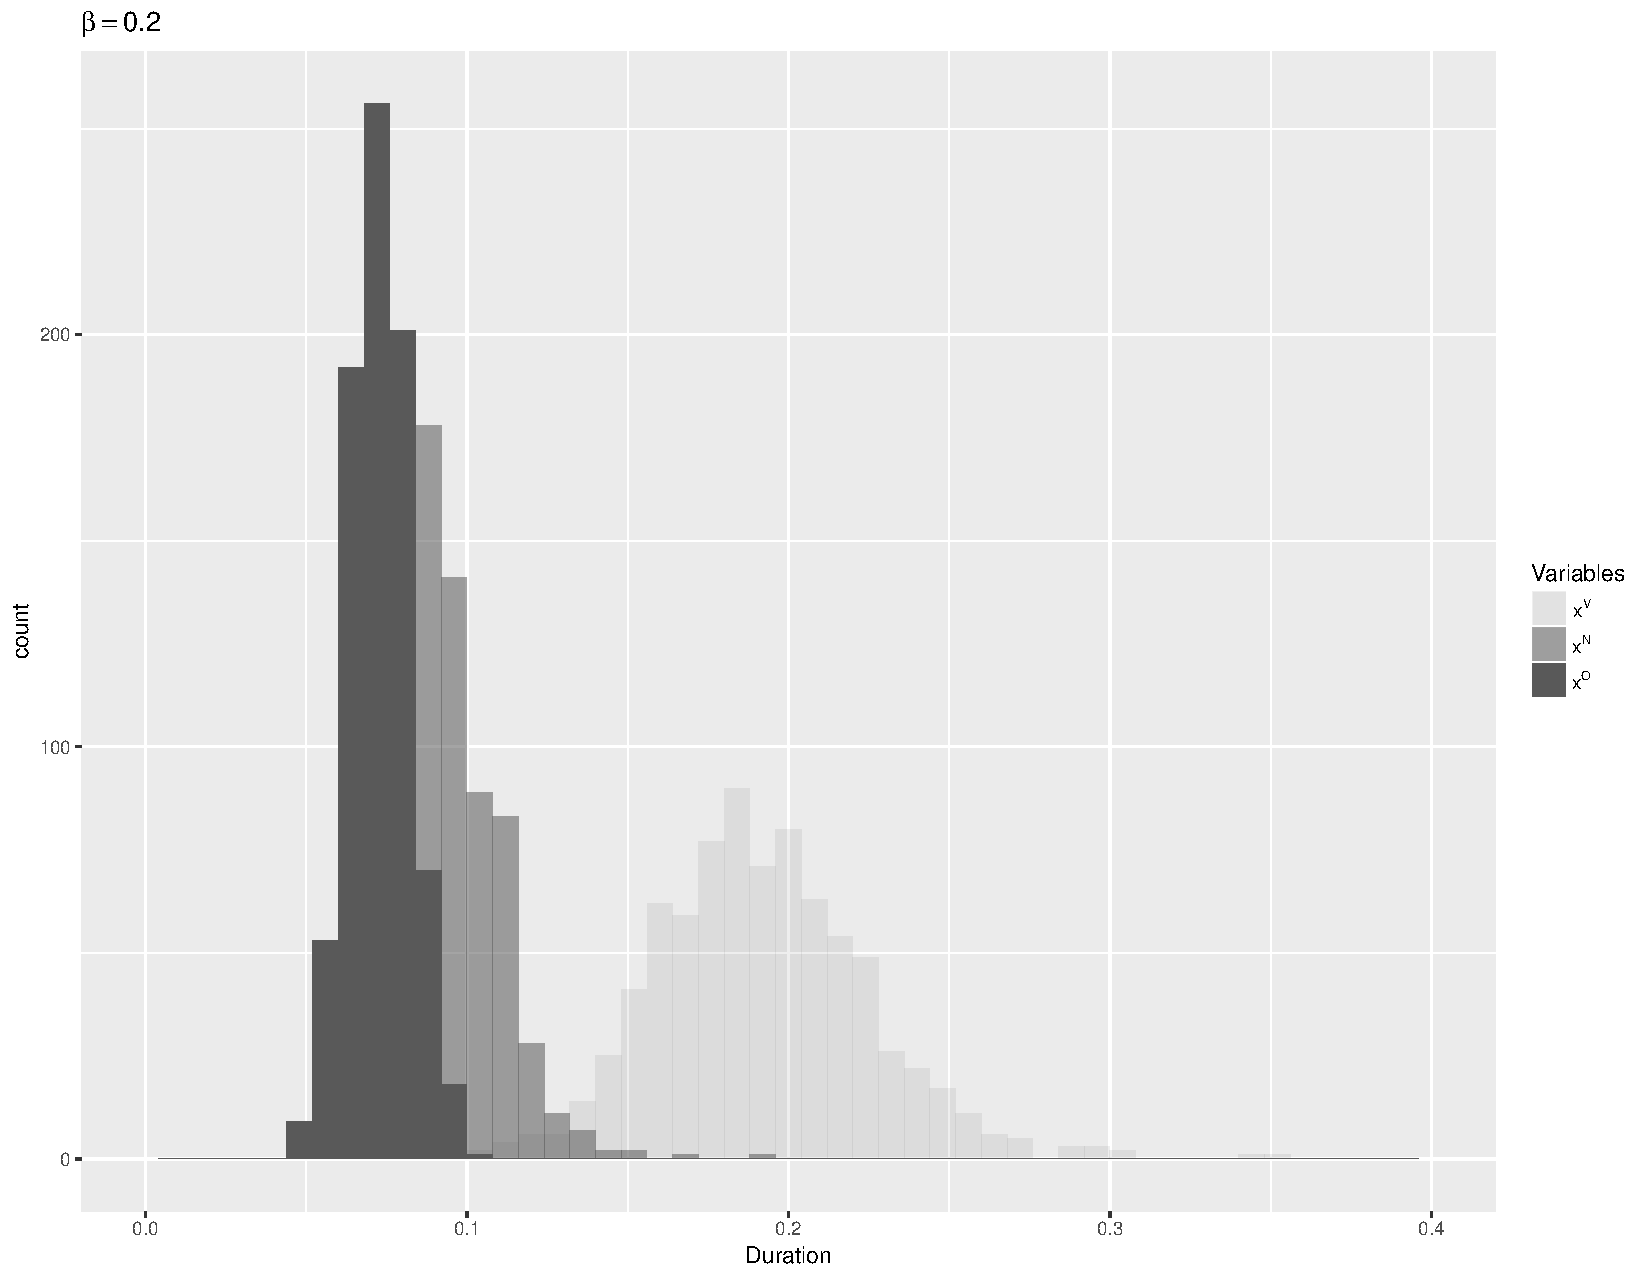
\includegraphics[width=\linewidth]{figures/SpeakingRateFrequencybeta2.pdf}
        \caption{Mid-frequency word ($\beta=.2$)}
    \end{subfigure}\hfill
    \begin{subfigure}[t]{.3\textwidth}
        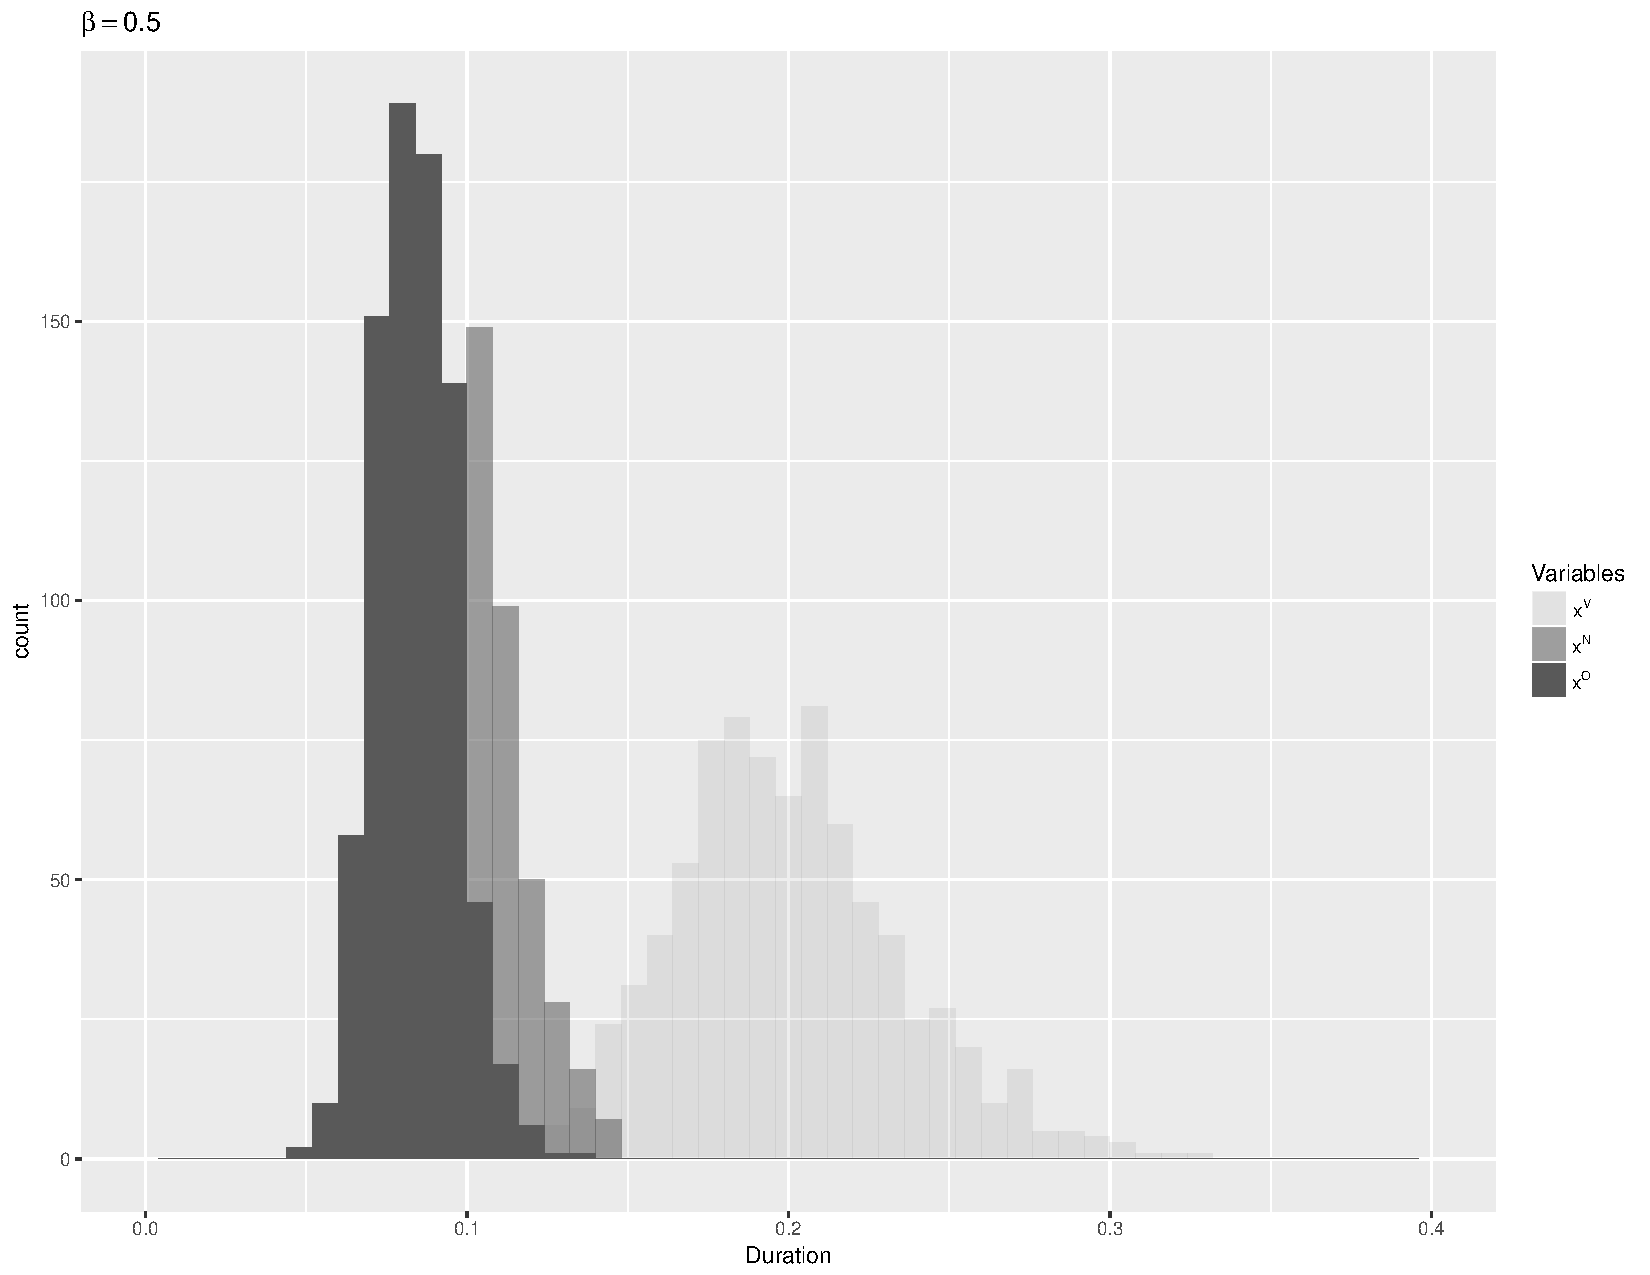
\includegraphics[width=\linewidth]{figures/SpeakingRateFrequencybeta5.pdf}
        \caption{High-frequency word ($\beta=.5$)}
    \end{subfigure}

% % % \subfloat[Low-frequency word ($\beta=.05$)]{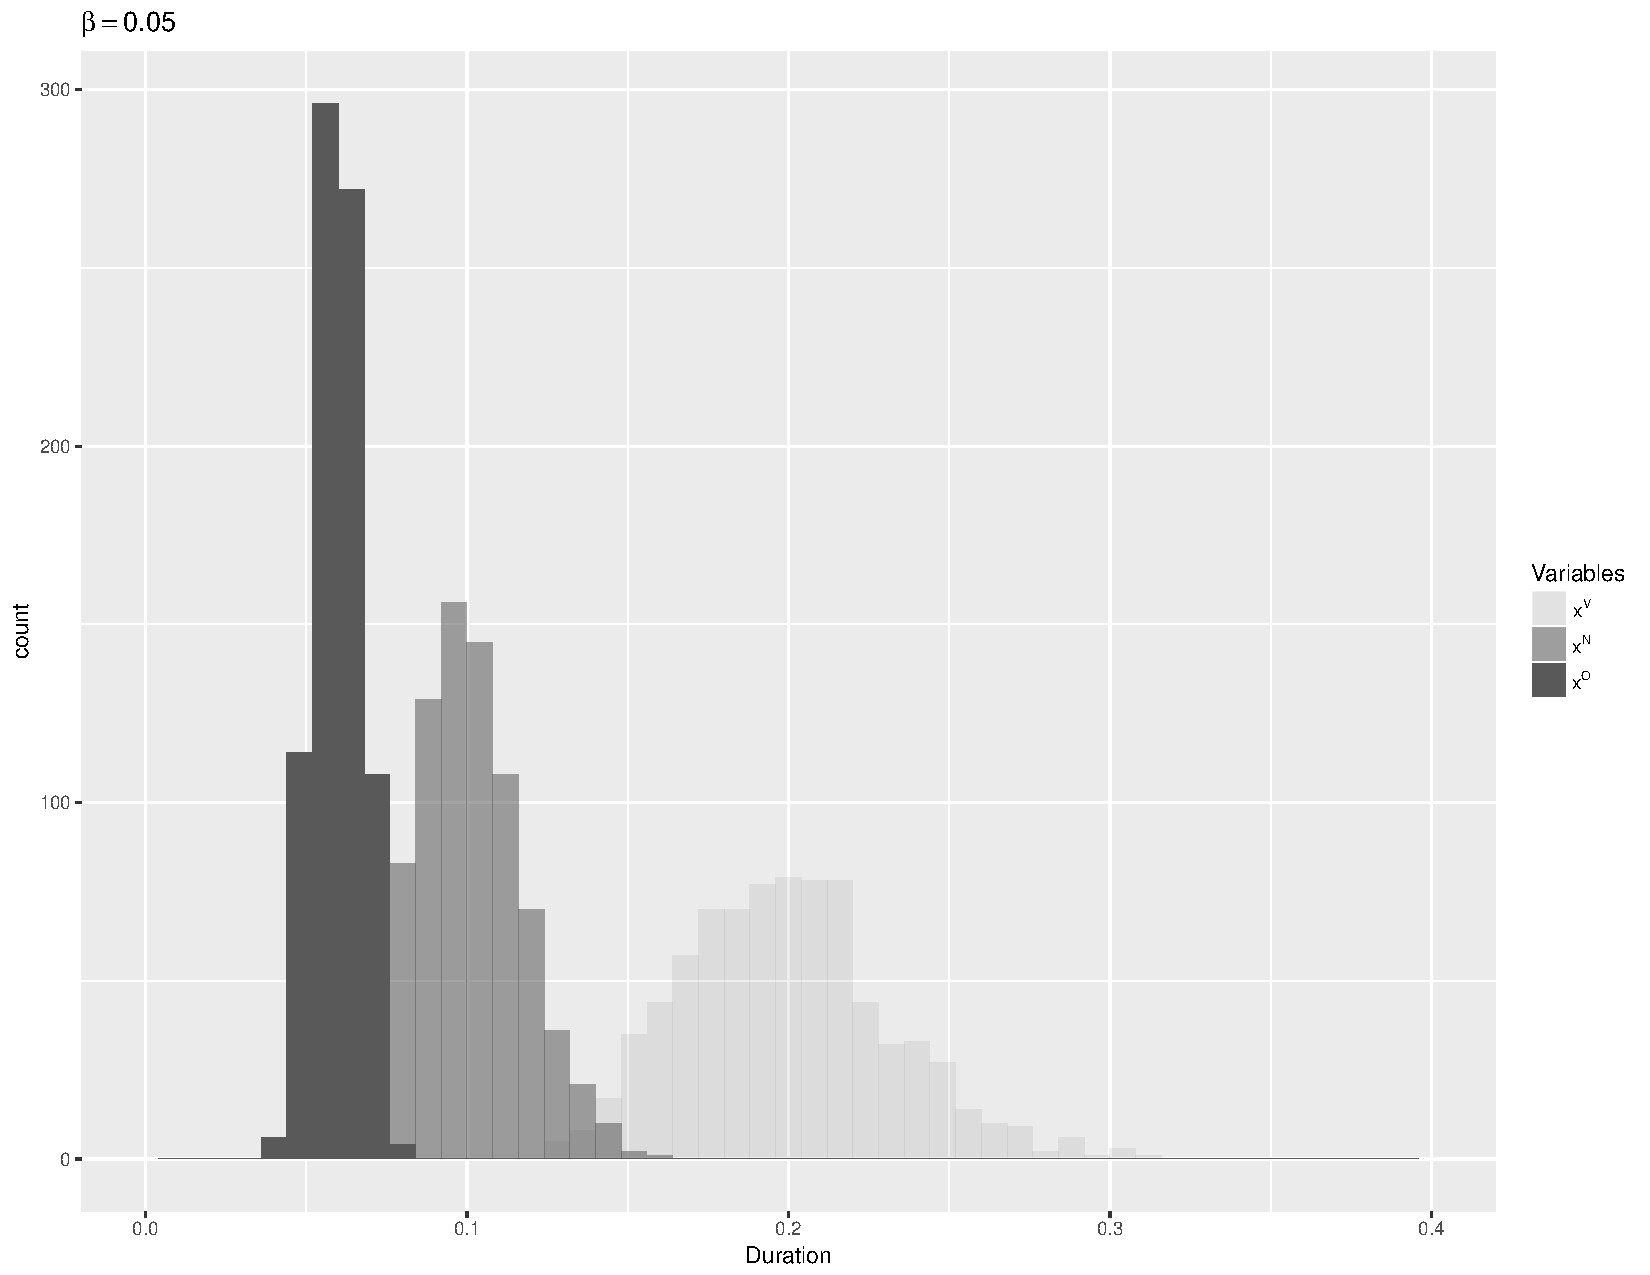
\includegraphics[width=0.25\textwidth]{figures/SpeakingRateFrequencybeta05.pdf}}
% % % \subfloat[Mid-frequency word ($\beta=.2$)]{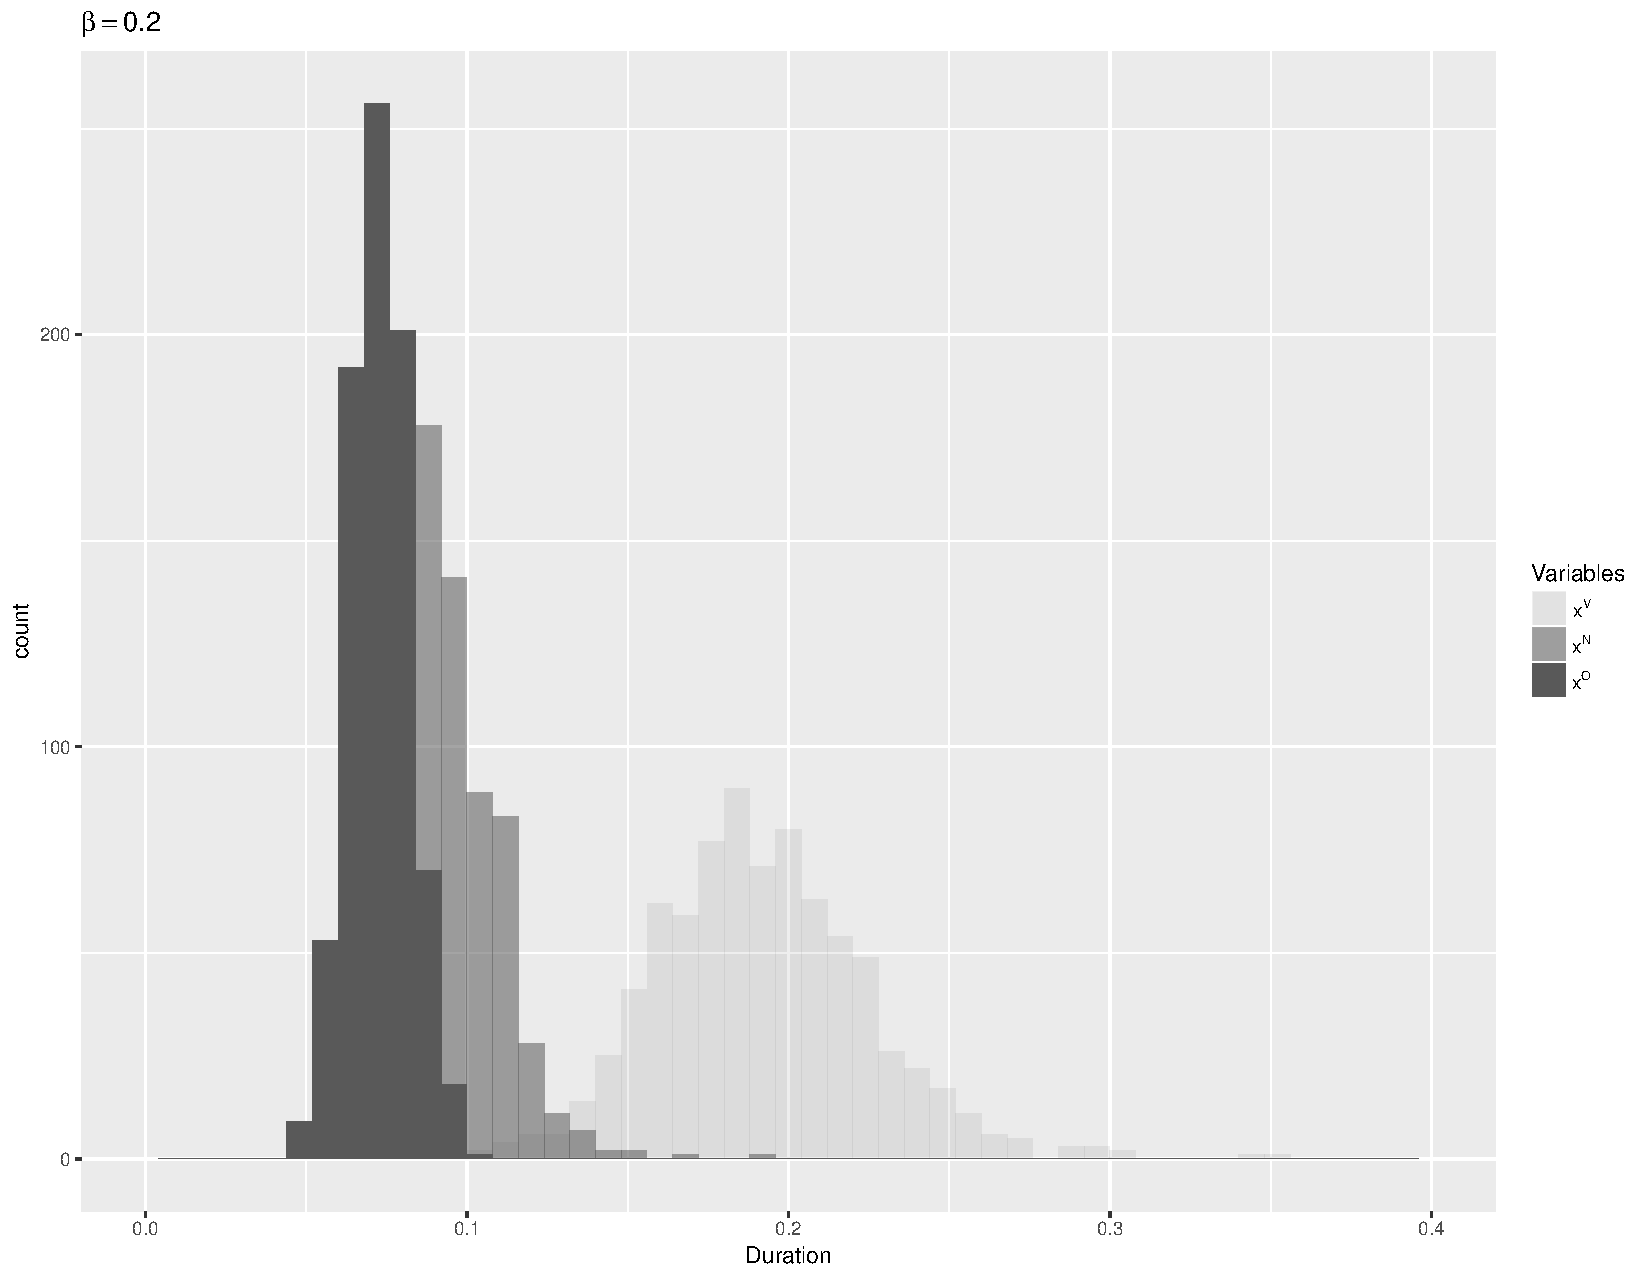
\includegraphics[width=0.25\textwidth]{figures/SpeakingRateFrequencybeta2.pdf}}
% % % \subfloat[High-frequency word ($\beta=.5$)]{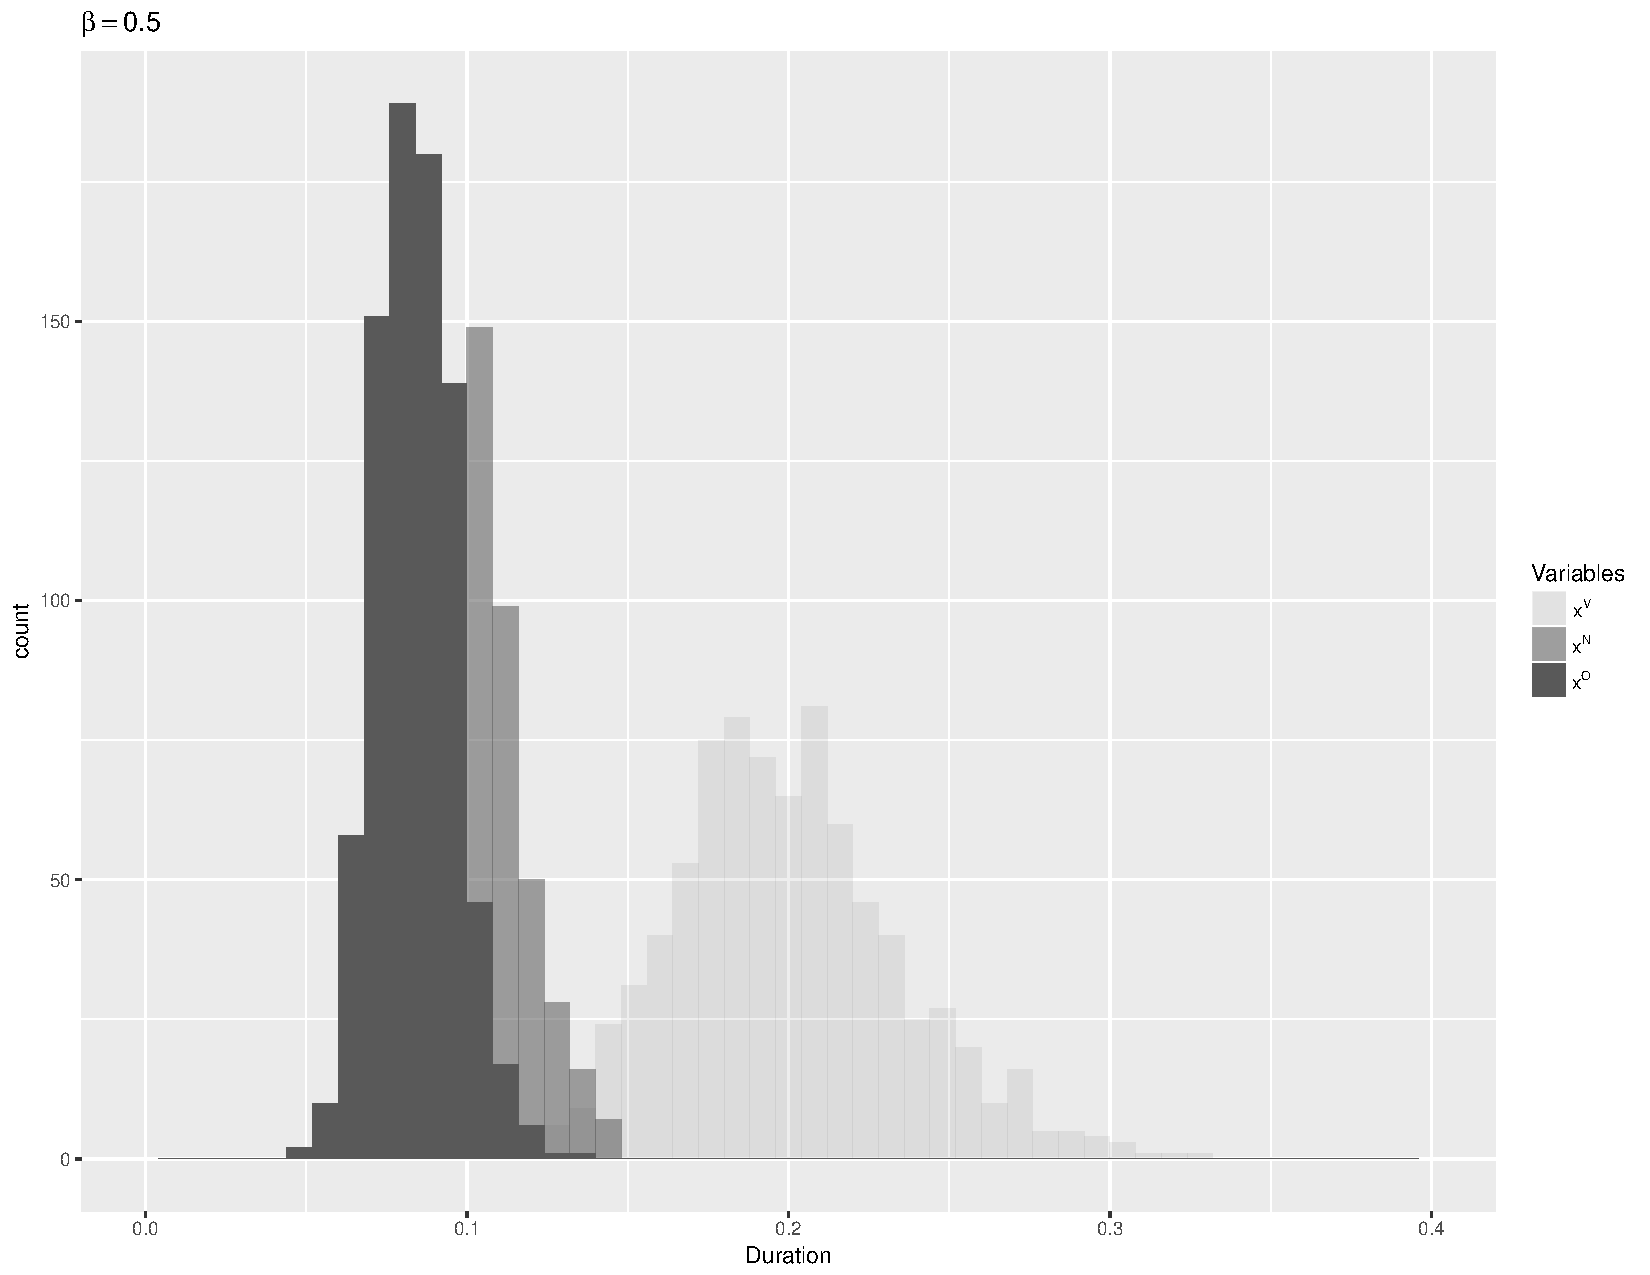
\includegraphics[width=0.25\textwidth]{figures/SpeakingRateFrequencybeta5.pdf}}


\caption{\label{fig:NasalizationModel1}No-Phoneme Phoneme-Split Model (Frequency
Attractor). Each model run for 10,000 cycles with identical starting conditions. }
\end{figure}

The No-Phoneme Phoneme-Split model predicts that words with higher
frequencies should be produced, on average, with vowels that are more
nasalized (larger degree of overlap between gestures), than lower
frequency words. It also shows that it is possible to achieve stable
phonetic change from a change in word frequency. The model implements
a theory of nasal vowel genesis as an emergent property of gradient
effects acting directly on articulatory parameters. Only in the special
case where overlap is roughly equivalent to nasal duration, would
the data likely be analyzed (by a linguist) as the result of phoneme
split. This state in the model, however, has no special status. And
distributions that appear intermediate with regard to the average
ratio of overlap duration to velum gesture duration can be stable.
Conceptualizing phoneme split in this way allows us to avoid the actuation
paradox that requires the loss of the conditioning environment, but
the retention of the conditioned allophone (see \sectref{sec:Actuation-1}).
In fact, as there are no phoneme-level representations in this model,
there are no allophones, and no conditioning environments, in the
classical sense. Therefore, this model is also a demonstration that
phoneme-level representations are not necessary (nor is any misperception/misarticulation
pressure of the kind discussed in the previous chapter), to achieve
a working model with the generally correct behavior. 

The source of the nasalization effect in this model is the coordination
between the tongue body and velum gestures. This parameter, however,
is part of the underlying specification of each word token. The No-Phoneme
model is thus a \noun{state} model. Arguably, a \noun{state} model
represents a change that has already taken place, in which a process
of nasalization has been reinterpreted as a static property of a unitary
representation. In the next sections we will turn to a \noun{process}
model of vowel nasalization, returning to the misperception/misarticulation
actuation mechanism. This will also involve introducing a sub-lexical
level of representation, and revisiting the implementation of word
frequency.

\section{Parsing and misparsing}

In order to recover the meaning of a given speech signal, it is necessary,
at minimum, to identify the individual lexical items present. This,
in turn, requires determining where one word ends and the next begins.
The highly context-sensitive nature of acoustic cues, as well as the
lack of consistent silence, or other markers, of the boundaries between
words or sounds, make this a computationally difficult task. And this
is not just an acquisition problem. Signal parsing, or segmentation,
is something that must be carried out every time speech is perceived. 

That segmentation of some kind must also take place at the sub-lexical
level is evidenced by a large literature on what are known as “trading
relations”, in which the value along a given phonetic dimension
that separates two members of a phonemic contrast is shown to vary
depending on the values of the other phonetic cues present. And those
other cues that influence the boundary location are not just those
that occur within the segment itself. For example, a given phone ({[t]})
may be ambiguous as to whether it belongs with a preceding or following
word (e.g. “great ship” {[}{ɡɹe͡ɪt}\#{ʃɪp}{]}
versus “gray chip” {[}{ɡɹe͡ɪ}\#{t͡ʃɪp}{]}),
and the actual word sequence that is heard will depend on the durations
of the surrounding segments; longer durations of {[e͡ɪ]}
increase the likelihood of “gray” over “great”, while
shorter durations of {[ʃ]} increase the likelihood of “chip”
over “ship”. An acoustic cue (such as silence itself) may also
be ambiguous as to whether it originates from a phoneme ({/t/})
or a break between words (“great ship” versus “gray ship”
{[}{ɡɹe͡ɪ}\#{ʃɪp}{]}; longer durations of silence
increase the likelihood of “great” over “gray” (\citealt{repp1978perceptual}).
An acoustic feature may also be ambiguous as to whether it belongs
to a preceding segment, a following segment, or both ({[}{ɹa͡ɪpbɛɹiz}{]}
as either “right berries” or “ripe berries” \citealt{Gow2003}). 

In all of the preceding examples the ambiguity exists because of the
existence of multiple real-word alternatives. Without those alternatives,
or competitors, phonetically ambiguous input quickly becomes perceptually
unambiguous (e.g. \citealp{warren1970perceptual,ganong1980phonetic}).
The strong susceptibility of low-level perception to high-level expectations
also speaks to the amount of noise, or essentially unpredictable variability,
in the acoustic realization of a given abstract category. Speech perception
involves the complex integration of multiple cues, each of which,
in isolation, may be relatively uninformative, in order to arrive
at a single parse, a single percept, of what is heard. This percept
is presumably the best alternative among those available to the listener
(see \citet{davis2007hearing} for a review of the literature). Although
speech perception appears extremely robust due to the fact that the
meaning intended by the speaker is usually recoverable by the listener,
that robustness is a property of the entire set of cues available,
not of acoustic features alone, and certainly not of individual acoustic
features. Rather than conceptualizing sound change as the relatively
rare event in which the listener mishears, or the speaker misspeaks,
it may be the case that what we typically think of as the “changed”
variants are already present within the distribution of stored tokens,
as one of multiple possible parses of each inherently ambiguous input
signal.

\section{Multiple parses}

The classical way in which sound change is conceptualized is based
on the assumption that there exists a unique, correct, sub-lexical
representation for each word. It is meaningless to speak of phoneme-level
“errors” unless this is the case. Consider the following hypothetical
example (where \emph{$x>y$} indicates an historical change from \emph{x}
to \emph{y}):
\begin{covexamples}
\item \label{anpa>ampa}\emph{anpa \textgreater{} ampa}
\end{covexamples}
(\ref{anpa>ampa}) is a common type of change known as nasal place
assimilation. In this example, the coronal feature of the nasal $/n/$
is assimilated to (or replaced by) the labial feature of the following
$/p/$. Speakers of a language that undergoes this change presumably
had an earlier allophonic rule specifying that $/n/$'s preceding
stops take on the place features of that stop. Therefore, the change
could only have occurred if they uncharacteristically failed to account
for this rule, or they made the “wrong” choice for a production
that was especially strongly assimilated. In either case, listeners
are assumed to parse their acoustic input into a sequence of discrete
phones, deciding for each segment whether to normalize or accept at
face value. Thus, for a change from \emph{/anpa/} to \emph{/ampa/}
to have actually occurred in the way it is denoted here, it must be
the case that listeners used to routinely segment continuous acoustic
tokens of this word into the sequence of units \emph{/a/}, \emph{/n/},
\emph{/p/}, \emph{/a/}, until they switched to segmenting
those tokens into the sequence \emph{/a/}, \emph{/m/}, \emph{/p/},
\emph{/a/}. 

Of course, we know that a discrete series of abstract symbols (either
\emph{[anpa]} or \emph{[ampa]}) is not present in the acoustic
signal in any objective sense. The abstract notation also implies
that this change occurs once, simultaneously, for all words, and for
all word tokens. However, adopting the hypothesis that multiple experienced
instances of speech are stored implies that change would have to occur
over individual tokens. In fact, the multiple-parse hypothesis is
a logical consequence of the basic tenet of the exemplar framework.
The conflation of perception and production that we saw in the exemplar models of Chapters~\ref{ch:The-Exemplar-Model} and~\ref{ch:Models-of-Change}
is borrowed directly from the standard generative notation. Once a
transformation from perceptual tokens to production tokens is required,
it becomes clear that 1) parsing is necessary in the first place,
and 2) it must occur for each experienced token. Recognizing
that acoustic tokens are inherently ambiguous with respect to their
decomposition into discrete units suggests, in turn, that variable
parses might be the norm rather than the exception.\footnote{This is closely related to the proposal that stored lexical items
can have more than one representation (see, e.g. \citealp{hooper1976word,Janda2008,Bybee2001}).
Split representations are also assumed to be the outcome of discontinuous
articulatory change in the model of \citet{Garrett2013}.} 

In the nasal assimilation example, there are two obvious alternative
parses, differing in whether they contain the phoneme $/n/$ or $/m/$,
thus the word-level category “anpa” is hypothesized to be composed
of at least some tokens specified with production targets for $/n/$,
and some for $/m/$. However, additional possible parses exist if
we do not assume the available phoneme inventory \emph{a priori}.
In fact, if we allow all universally possible segments into the analysis
space, then we avoid the actuation paradox of the classical diachronic
approach. As the next section will show, this re-framing of the change
question allows synchronic variation to be linked to diachronic change
in a way that is not dependent on either stopping or starting the
model at a critical point in time. 

\section{Representations II}

The Multiple-Parse model adds a \noun{process} component to the No-Phoneme
model. The process is implemented at the level of the articulatory
gesture, but conceptually requires the existence of abstract categories
intermediate between the word and the gesture. As before, the change
occurs in the distribution of variants that already exist, rather
than in the genesis of entirely novel forms. This aspect bears some
similarity to the proposal in \citet{Baker2011}, based on misanalysis
of the signal, but the current model is not abrupt, nor does it require
“extreme” variants to be adopted.

The conversion from perception to production is the locus of sub-lexical
parsing, mapping every continuous acoustic token into a series of
categorical units. In principle, these units can consist of any contiguous
set as long as it is phonetically plausible, and exhaustively parses
the input signal. However, in the case of vowel nasalization, we will
be concerned with two particular possibilities: the one-sublexical-unit
analysis, and the two-sublexical-unit analysis. These are of special
interest, of course, because they bear considerable similarity to
the classical analyses of the phenomenon before change (two units),
and after change (one unit). However, it is important to be very careful
in how these units are described, because the traditional notational
system essentially forces an analysis more general than the
word level. In order not to assume generalization, and remain representationally
consistent, the following notation will be adopted for the two sub-lexical
parses of the word in question (“am”): $/\tilde{V}_{am}/$ (Analysis
1), and $/V_{am}/+/N_{am}/$ (Analysis 2). The desired implication
is that only after generalization across multiple words could something
similar to the abstract categories $/\widetilde{V}/$ and $/V/+/N/$
arise.

For the articulatory parameters already defined, a single-unit parse
means that all three values will be stored on the production side.
$/\tilde{V}_{am}/$ is a 3-dimensional cloud, and entrenchment applies
over each dimension. Note that this is what was assumed for all tokens
in the No-Phoneme Model, which therefore implicitly assumed a single-unit
analysis. The two-unit parse, however, is explicitly a \noun{process}
analysis, entailing that one token is drawn from a one-dimensional
\emph{$/V_{am}/$} cloud, one from a one-dimensional \emph{$/N_{am}/$}
cloud, with concatenation occurring at the time of production. In
other words, the overlap between the two gestures is not stored, but
determined online. 

\section{Multiple-Parse Phoneme-Split Model}

Either analysis is possible for any given token, but, critically,
depends on the acoustic properties of that token. In this set of simulations
it will be assumed that word-level categorization is correct, and
that the three duration quantities ($x_{i}^{V},x_{i}^{N},x_{i}^{O}$)
are accurately recovered in perception, although this is not critical.\footnote{If the error term is symmetrical, then it will have no qualitative
effect on the model dynamics.} Analysis 1, the single-segment analysis, is more likely to be selected,
the more highly overlapped the gestures that produced that token,
while Analysis 2, the 2-segments-in-sequence analysis, is more likely
for less overlapped gestures. The specific dependence is on the quantity
$Q_{i}={x_{i}^{O}}/{x_{i}^{N}}$. Larger values of $x_{i}^{O}$
lead to larger values of $Q_{i}$, as do smaller values of $x_{i}^{N}$.
Selecting for large \emph{Q} thus selects both for larger overlap
and shorter word durations. That duration should correlate with number
of constituents is a reasonable hypothesis. It can also be hypothesized
that articulatory gestures will tend to be more tightly coordinated
within, than across, segments, if shared constituency promotes greater
merger.\footnote{I am not aware of evidence for this specific relationship, but there
is evidence for different types of gestural coordination across different
domains: between the onset and nucleus of a syllable, versus the nucleus
and coda (\citealt{Browman1988,byrd1996influences}); and within,
versus across, morpheme boundaries (\citealt{Cho2001}).} The probability of Analysis 1, $P(a=1)$, depends on \emph{Q} in
the following way (\ref{eq:segmentation-1}).
\begin{equation}
P(a=1)=Ae^{-b(1-Q)}-C\label{eq:segmentation-1}
\end{equation}
Probability increases with increasing \emph{Q} because of the negative
exponential in (\ref{eq:segmentation-1}). The largest possible value
for \emph{Q} is 1, therefore $1-Q$ is always positive. When $Q=1$
, $P(a=1)$ reaches its maximum at $A-C$. How quickly the probability
decreases as a function of decreasing \emph{Q} is controlled by the
variable \emph{b. }The larger \emph{b}, the larger the negative exponential,
and the more quickly $P(a=1)$ decreases, selecting for larger mean
\emph{Q} values (and fewer tokens). See Appendix \ref{chap:Appendix E}
for additional details.

If Analysis 1 is chosen in perception, based on the value of $P(a=1)$,
then all three values of the token are stored. If Analysis 2 is chosen,
then the duration of the tongue body gesture ($x_{i}^{V}$), and the
duration of the velum gesture ($x_{i}^{N}$), are each stored in separate
categories, and the overlap value is discarded. Figure \ref{fig:MultiParse-Reps}
provides a schematic depiction of these relationships. Note that the
dimensions are not accurately represented here; two dimensions are
used for all categories to make the membership relationships easier
to see. Individual tokens are drawn as schematic gestural scores:
extent represents time, and fill type represents active articulator.
Where the two bars appear together, horizontal alignment indicates the stored gestural overlap parameter. The thin
lines drawn between tokens of different sub-categories indicate that
they are stored together, and will be produced together. However, overlap must
be determined separately because it is not stored as part of the experienced token. Entrenchment happens only
within individual sub-lexical categories.\footnote{If entrenchment at the word level is added it will have the effect
of pushing values back towards the means of the Analysis 2 categories,
since the model is initialized with those values, and the Analysis 2
parse is always more likely.}

\begin{figure}[h]

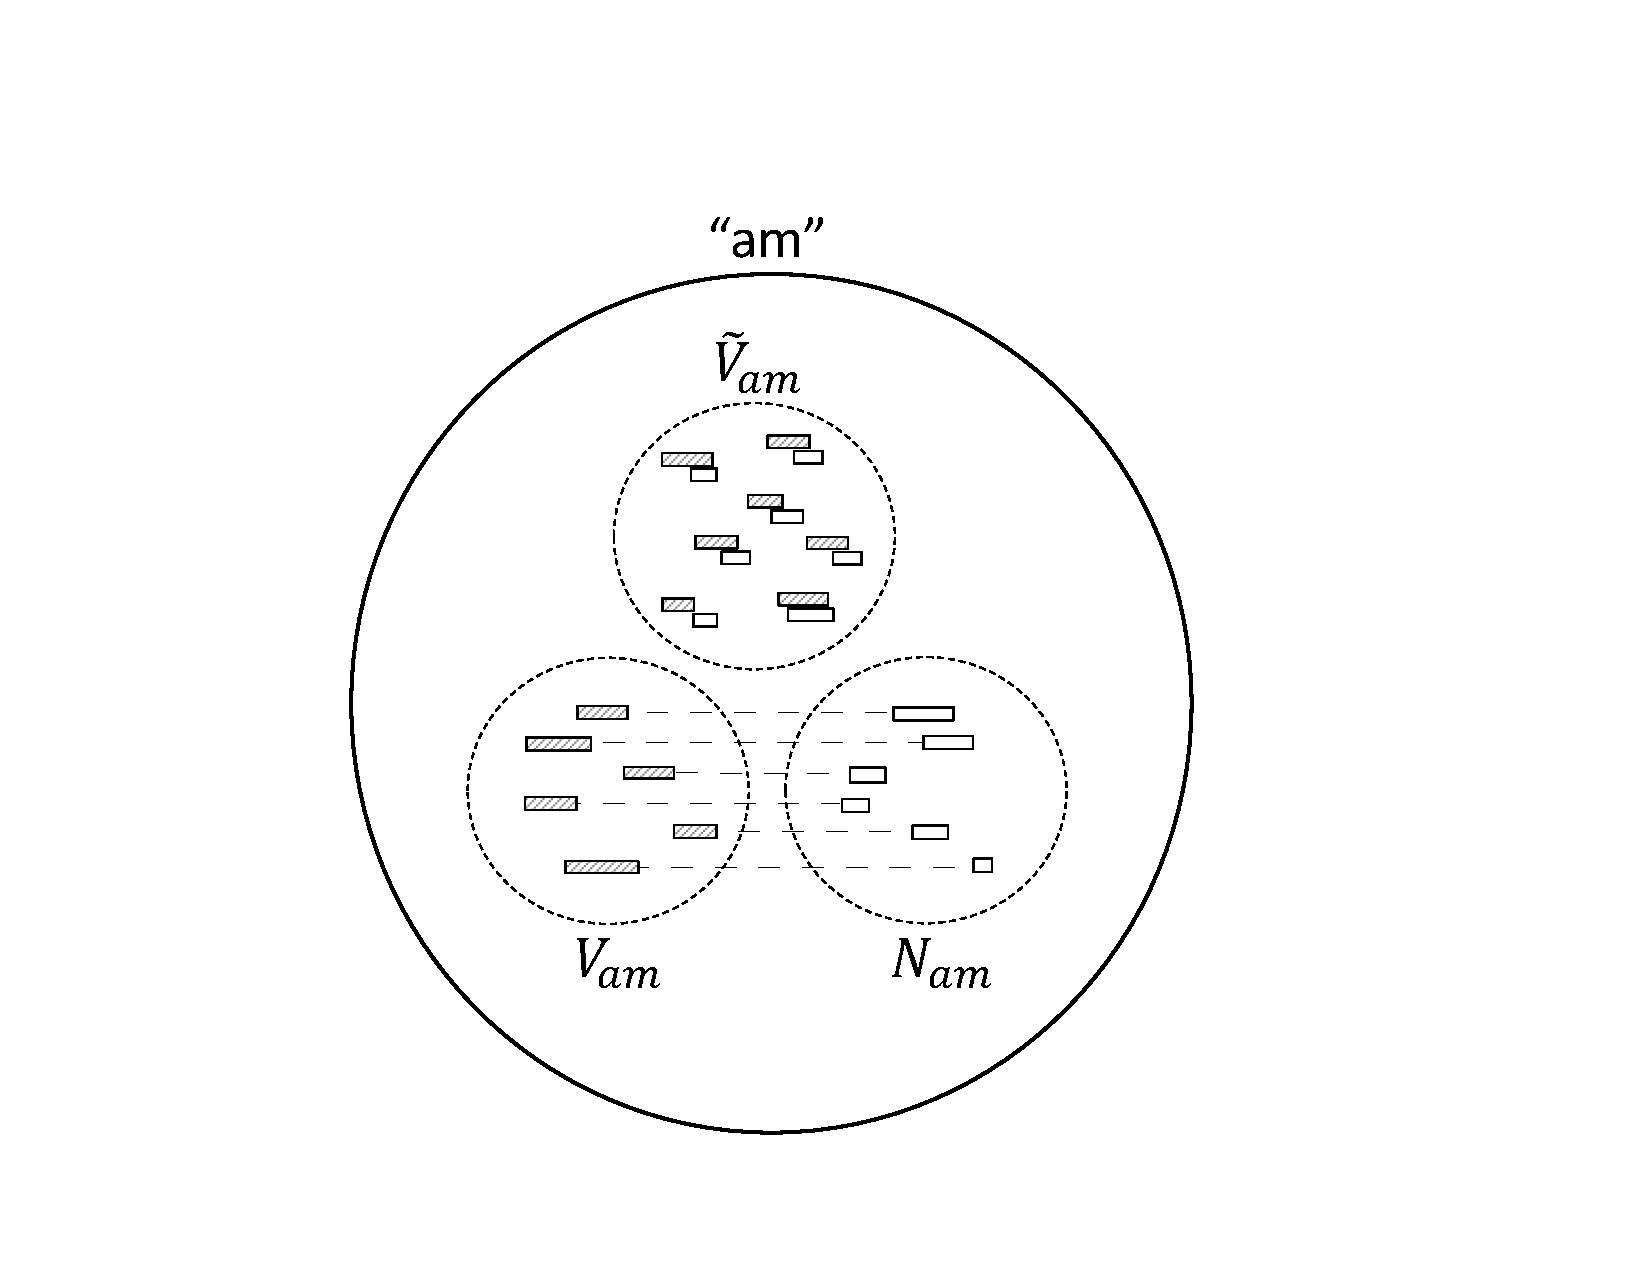
\includegraphics[width=0.6\textwidth]{figures/MultiParseModel.pdf}\caption{\label{fig:MultiParse-Reps}Schematic depiction of the relationships
between the word-level category (“am”) and the sub-lexical level
categories of its constituents. Production-side representations.}

\end{figure}

Tokens are chosen randomly for production from among all stored values.
Once selected, the token is subject to the same speaking rate transformation
used in the No-Phoneme model. The overlap degree for an Analysis-2
token defaults to a fixed percentage of the current average value
of $x^{N}$ (with some variance). There is no phonetic bias in this
model. The selection bias that drives the feedback loop resides in
the choice of underlying analysis – the parsing of the input signal.
Equation~\ref{eq:segmentation-1} selects for large values of $x^{O}$,
and for small values of $x^{N}$, both of which will increase the
size of \emph{Q}, and thus increase the probability of Analysis 1.
There is no cumulativity such that these values grow more extreme,
but there is a constant pressure to sort tokens with the largest overlap
proportion into this sub-lexical category. Thus, if an independent
mechanism resulted in an increase in \emph{Q} for some tokens, those
tokens would raise the average \emph{Q} value of the $/\tilde{V}_{am}/$
sub-category.

A mechanism that shortens word duration will have this effect: shortening
$x^{N}$ (and $x^{V}$), and lengthening $x^{O}$. If higher frequency
is taken to result in faster productions, then an increase in frequency
will lead both to more $/\tilde{V}_{am}/$ categorizations, and to a higher \emph{Q} value for the category on average. For the simulations
reported below, frequency was implemented as a negative perturbation
to the mean value of the expansion force distribution. As a result,
higher frequency (higher resting activation) results in shorter words,
and thus shorter tongue body and velum gestures (and longer overlap)
under all speaking rates. This implementation will be discussed in
more detail in the following section. 

Figure \ref{fig:Multiple-Parse-Results} shows the model results as
a function of frequency. Each point is the result of running the model
for 10,000 iterations. Mean values for the three duration parameters,
as well as the proportion overlap (\emph{Q}) are given for each of
the categories - Panel 1: word-level; Panel 2: Analysis 1 tokens; Panel
3: Analysis 2 tokens. Note that the overlap proportion in Panel 3
shows the constraint that overlap proportion stay fixed with respect
to $\overline{x^{N}}$. Whereas, in Panel 2, as resting activation
(frequency) increases, the proportion overlap increases. Because the
number of tokens parsed into the $/\tilde{V}_{am}/$ category also
increases with increasing resting activation (from approximately 31\%
to 50\%), the overlap proportion increases for the word-level category
as a whole (Panel 1). 

\begin{figure}[h]
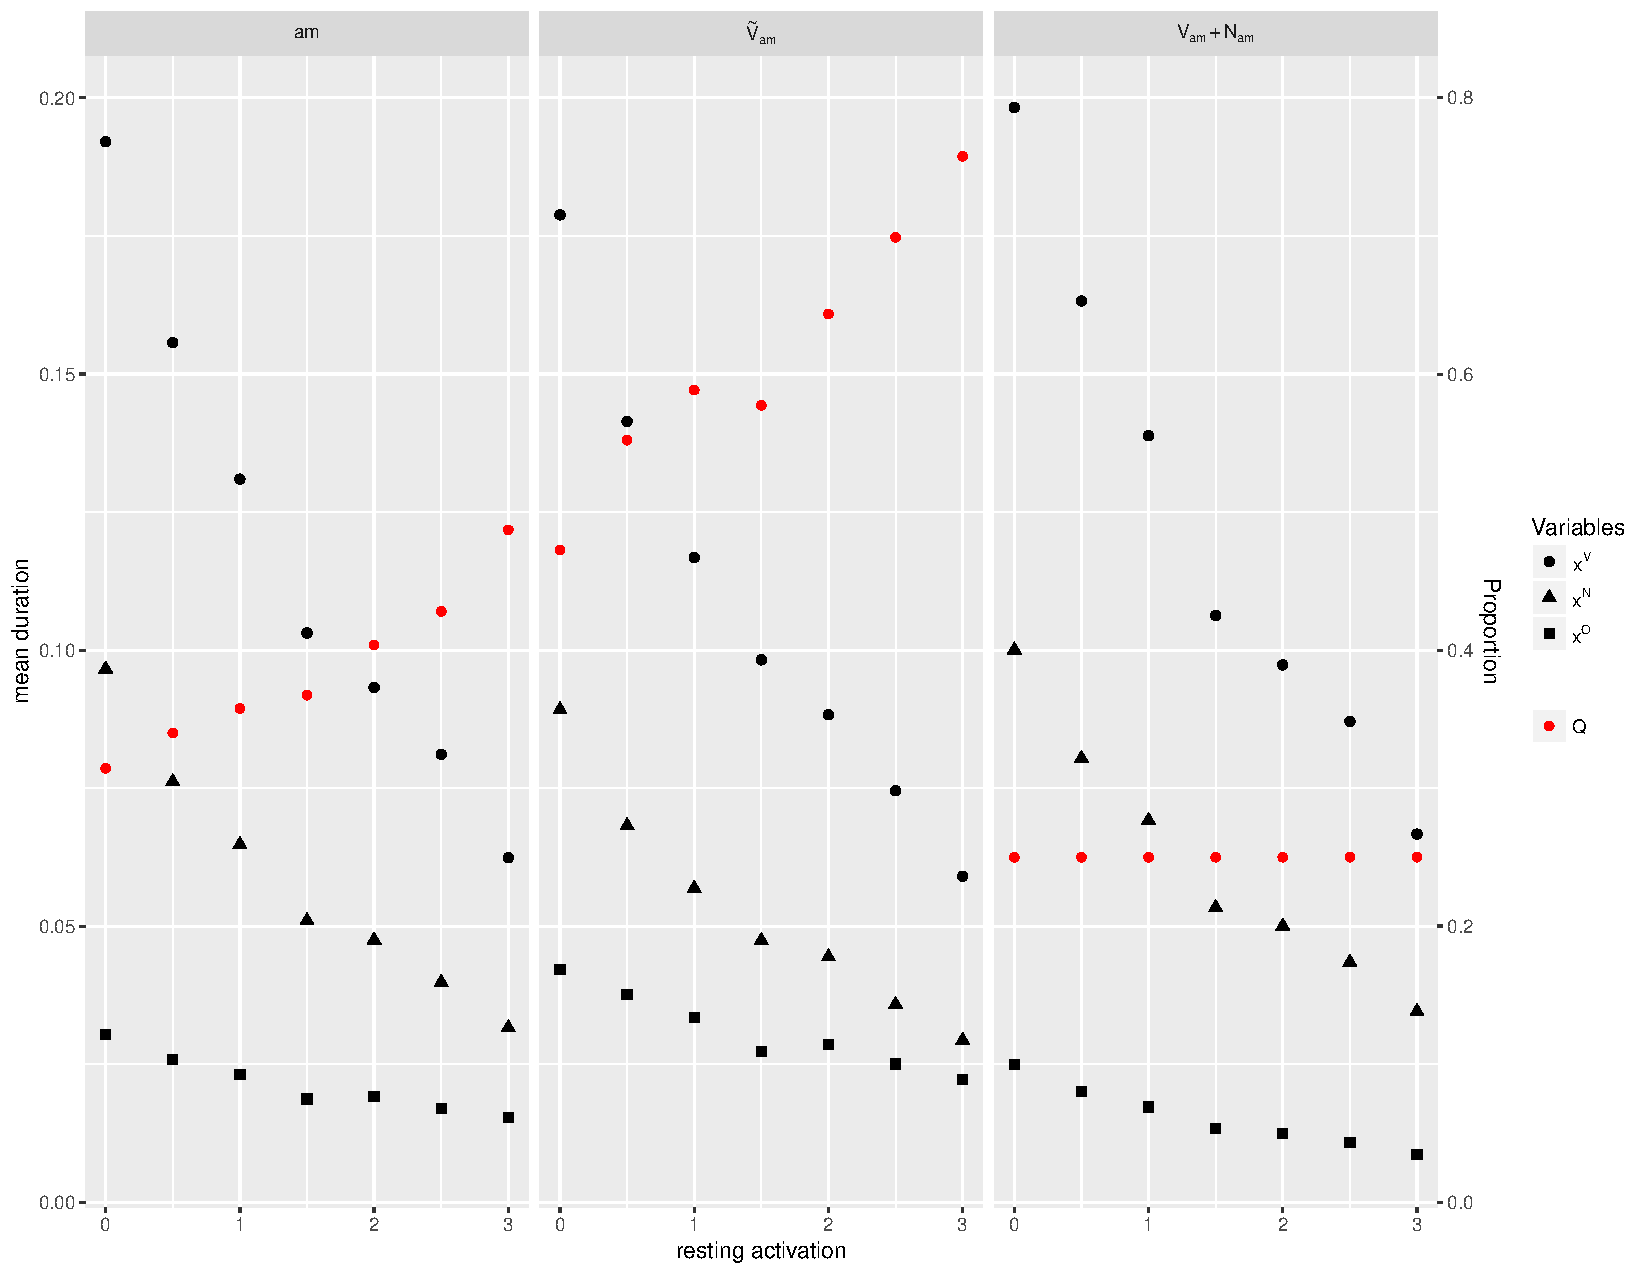
\includegraphics[width=.70\textwidth]{figures/MultipleParseResults.pdf}
\caption{\label{fig:Multiple-Parse-Results}Multiple-Parse Model: Results as
a function of resting activation (word frequency). Each point corresponds
to the mean after 10,000 model iterations. Mean articulatory durations
are plotted in black. Proportion overlap ($Q={\overline{x^{O}}}/{\overline{x^{N}}}$)
is plotted in red. Panel 1: all word tokens; Panel 2: Analysis-1 tokens
only; Panel 3: Analysis-2 tokens only.}
\end{figure}


\section{\label{sec:Frequency-II}Frequency II}

In the No-Phoneme Phoneme-Split model, frequency was implemented as
a fixed attractor on overlap duration (Section \ref{sec:Frequency-I}).
The assumption was that there existed an optimal (most fluent) production
of a given word with precisely the degree of gestural overlap given
by the attractor target. At the same time, in order to generate productions
that more closely resembled nasal vowels, it was necessary to set
the target quite high – in the reported simulations it was set to
the entire duration of the accompanying velum gesture. However, it
is not clear why the optimal production of the 2-gesture word should
exhibit such a large degree of overlap. And, in general, there is
no clear reason for greater practice, or increased fluency, to always
result in shortened, or reduced, articulations, especially to the
point where distinctiveness may be lost at the word and/or phoneme
level. Yet this seems to be the case with frequency effects. It has
been shown, for example, that individual segments within high-frequency
words are shorter, and that they are more likely to exhibit “deletions”
(dropping, or masking of a consonant, or unstressed vowel, e.g.
\citealt{Bell2003,Raymond2006,Bybee2008}). The realizations of segments
in higher-frequency words tend also to be less extreme, or more “centralized”,
perhaps failing to reach the usual articulatory target (e.g. \citealt{munson2004effect,Scarborough2004,gahl2008time}).

The listener-based account of frequency effects explains these phenomena
as a consequence of contextual predictability. It is actually the
less predictable, less easy to access, more confusable, forms that
are produced with particular care (hyper-articulated) by the speaker
in order to aid intelligibility (e.g. \citealt{Aylett2004}). In
the absence of that pressure, articulations are reduced to the degree
possible, facilitating the task of the speaker. Factors that have
been shown to affect predictability, as well as word form, include
sentence, or discourse, context, bigram frequency, and unigram frequency,
among others. Nevertheless, there are a number of results that are
not compatible with a strictly listener-based theory, studies that
have shown that speakers do not always alter their productions in
such a way as to facilitate listener comprehension (see \citealt{turnbull2015assessing}
for a review of the literature).

As mentioned briefly in \sectref{subsec:Word-Frequency}, the
speaker-based approach attributes frequency effects to automatic production-side
mechanisms. This is usually couched in terms of activation levels,
within some kind of lexical network model where different representations
“compete” in both perception and production (e.g. \citealp{mcclelland1981interactive,Dell1986}).
In terms of word retrieval, the successful candidate is the one that
achieves a given threshold of activation first. Every time a word
is accessed, or produced, it is activated to this level. Repeated
activations, within some time period, are taken to result in some
level of residual activation that persists even when the word is not
selected. This “resting” activation level is naturally higher
in higher frequency words, giving them a head start against lower-frequency
competitors. 

The resting-activation account is in line with results establishing
that higher-frequency words are produced earlier than lower-frequency
ones in a variety of tasks, such as picture naming, and word or sentence
reading – even with delays. Higher-frequency words also lead to faster
response times in lexical decision and other speeded response tasks,
as well as to greater accuracy in word recognition (e.g. \citealt{howes1951visual,balota1985locus,Luce1986,Marslen-Wilson1990}).
However, it is not at all obvious that higher resting activation alone
can account for articulatory or temporal reduction (hypo-articulation).

In fact, it has been argued \emph{both} that a higher activation level
should lead to hyper-articulation (e.g. \citealt{Baese-Berk2009}),
and that it should lead to hypo-articulation (e.g. \citealt{gahl2012reduce}).\footnote{Note that different results were obtained in these studies, one based
on laboratory data, and one on conversational corpus data.} In works that adopt the latter position, the connection seems to
be assumed. For example, \citet[79]{gahl2012reduce}
write that “Production-based accounts ... would lead one to expect
that words that are retrieved quickly tend to be phonetically reduced
– \emph{provided that fast retrieval speed translates into fast production
speed”} (emphasis mine).

The fact that there does not appear to be a well-worked out mechanism
for this result raises the possibility that we have yet to find the
right model for frequency. Empirically, however, the correlation between
shorter/faster productions and higher word frequency seems quite robust.
In the Multiple-Parse Model, a frequency-based increase in production
speed is taken to be an additive effect, acting to effectively shift
the speaking rate distribution. If we continue to assume that speaking
rate acts independently of other model forces, then words will continue
to be pulled in both directions, expanding or compressing in turn.
Subject to the same large positive force, both low and high frequency
words will be produced more slowly, and will thus be longer than if
no force had applied. However, the high-frequency word will be somewhat
shorter than its low frequency counterpart, due to the difference
in its resting state. The same will be found under compression (unless
floor is reached).

The dependence on frequency (resting activation) in Figure \ref{fig:Multiple-Parse-Results}
shows the effect of progressively shifting the speaking rate distribution;
shorter average word durations result in shorter $x^{N}$, and longer
$x^{O}$, and thus lead to a greater proportion of Analysis 1 tokens.\footnote{Because the duration of overlap cannot exceed the length of the shortest
gesture, the longest \emph{absolute} overlap durations can only occur
with the longest word tokens, thus there is also some selection pressure
towards longer $x^{N}$ inherent in the $x^{O}$ measure. Reducing
the length of $x^{N}$ will therefore eliminate some of the largest
$x^{O}$ tokens.} This shift is not unbounded, because speaking rate is a bi-directional
force; high-frequency words can also be lengthened, just not lengthened
quite as much as their lower-frequency counterparts. Note that the
frequency effect in this model acts on all tokens, both stored and
generated. In the latter case, we must assume that some type of motor
plan involving the concatenation of $/V_{am}/$ and $/N_{am}/$ is
associated with a resting activation value that affects the duration
of the resulting word. 

\section{Actuation}

As in the No-Phoneme Phoneme Split model, there is no single moment
at which a sound change occurs in the Multiple-Parse Phoneme-Split
Model. Every instance of perception involves a decision about parsing
which is based on existing synchronic variation. And every available
parse is a possibility at any time, for any token; it is the probabilities
of those parses which change over time. Although the nasal vowel parse
is assumed in the sense that it is one possible analysis for a given
token, this model, in fact, avoids many limiting assumptions about
the nature of sound change inherent to the classical view. For example,
the \emph{/V+N/} analysis is not privileged, beyond having a higher
probability of selection, given the starting distribution. Additional
analyses can be added to the set of parsing hypotheses, if motivated
by general-purpose properties of speech perception. It is consistently
the word level at which all forces act in this model, and at the level
of articulatory gesture that changes are realized. In particular,
this model does not rely on the allophonic level at which the synchronic
rule, and the diachronic change, are assumed to occur. As a result,
the normalization/lack of normalization question becomes a basic element
of speech processing: the analysis that must occur when perceptual
values are transformed into production values. 

If classification occurs at the word level, and words have articulatory
representations something like gestural scores, then it is not necessary
to first identify a series of abstract phonemes in order to identify
individual words. Thus, the problem of “compensating” for (the
feature of) nasalization at the level of the phoneme disappears. The
ambiguity remains regarding the proper articulatory realization of
a given acoustic input, but there is no longer a unique, correct sub-lexical
analysis. The possible analyses available to the listener, based on
their phonetic experience, should always include, at minimum, both
the “normalized” option, as well as the “unnormalized”
one.

In the specific simulations reported in the previous section, the
average percentage of the velum lowering gesture that occurred simultaneously
with the tongue body gesture varied from 30\%, for the lowest-frequency
word, to about 50\% for the highest-frequency word. It was also the
case that absolute gesture durations were considerably shorter
at higher frequencies. These results describe a diachronic change
under the scenario in which a single word comes to be used more, or
less, frequently over time. Under the scenario in which frequencies
are fixed, but there exists a set of words with a range of different
frequencies, these results describe a synchronic distribution. The
model thus generates at least two testable predictions: 1) that a
difference in the degree of vowel nasalization should be observed
across words of different frequencies (provided the relevant phonological
context is sufficiently similar among those words), and 2) that the
highest-frequency words should approximate the degree of vowel nasalization
observed in languages that are described as having phonemically nasal
vowels. In other words, no exaggeration, or enhancement, of the effect
is required in this model. Lexicon-wide change is assumed to start
with change at the individual word level.

It is widely acknowledged that change (of certain kinds, at least)
happens on a word by word basis (e.g. \citealt{Phillips1984,Bybee2002,Pierrehumbert2002}),
and that some words can be ``further along'' in the change than others.
With regards to nasalized vowels in particular, \citet{malecot1960vowel}
offers evidence that the distinction between English words like “cap”
and “camp” is primarily that between a nasal and oral vowel
({[kæp]} vs. {[kæ̃p]}), rather than the presence
versus absence of a nasal consonant ({[kæp]} vs. {[kæ̃mp]}).
The English segmental inventory is not usually analyzed as containing
an abstract nasal vowel (although see \citealt{Sole1992} for an argument
that nasal vowels are phonologically specified). Nevertheless, individual
tokens, or individual words, or even classes of words, may have phonetic
realizations that are indistinguishable from those generated from
an underlying nasal vowel. 

\chapter{Discussion \& conclusions}\label{ch:Summary}

The aim of \chapref{ch:Phoneme-Split} was to develop an explanatory
model of a specific type of sound change: \isi{phoneme split}, or \isi{phoneme}
genesis. Yet, in the course of developing that model, the change being
modeled itself underwent a certain kind of transformation. When \isi{phoneme}
split was first introduced in \sectref{sec:Actuation-1} it was
described as \isi{allophone} becoming \isi{phoneme}. The implication, particularly
in the case of \isi{vowel nasalization}, was that a completely new \isi{phoneme}
category had to be created, something that had not been previously
modeled. The classical representations for the \isi{synchronic} and diachronic
rules are given below.
\begin{covexample}
\label{allophonic rule}$/V/\rightarrow[\tilde{V}]/$\_\_$N$
\end{covexample}
\begin{covsubexamples}
\item \label{split-1}$/VN/>/\tilde{V}/$
\item \label{split-2}$[\tilde{V}]>/\tilde{V}/$
\end{covsubexamples}
In scenario (\ref{split-1}), the loss of the nasal context \emph{(N)}
is the precipitating event, critical to the emergence of the \isi{phoneme}.
In scenario (\ref{split-2}) the loss of the nasal context is irrelevant;
the \isi{phoneme} arises through some other mechanism.

Immediately, the \isi{actuation} problem arises – the problem of determining
why \isi{phoneme split} sometimes happens and sometimes does not (\citealt{Labov1968}).
If the conditioning context can be lost without \isi{phoneme genesis}, then
it cannot be the loss alone that creates the \isi{phoneme} (\ref{split-1}).
But if the loss of context is irrelevant and coincidental, then contextually
predictable phonemes are possible and we have no way to determine, or predict, the status of such sounds (\ref{split-2}).

The solution to this impasse suggested by the Multiple-Parse
Model is that phonemes are nothing other than hypotheses made by individual
listener/speakers about how to break up word-level units, hypotheses
that may change from moment to moment and from token to token. Once
such a hypothesis is made it acquires its own representational reality
– at least for that listener/speaker. Because \isi{allophonic} relationships only
exist as corollaries of a given phonemic analysis, they are automatically
generated under one hypothesis, and automatically missing under the
other. 

However, even under the “\isi{allophonic}” analysis, allophones never
actually surface in this model. The process that generates what linguists
would label as an \isi{allophone} does not occur at the same representational
level as the \isi{phoneme}; it occurs in the region shared between two adjacent
phonemes.\footnote{Incidentally, this reveals another hidden assumption of the generative
notation: the fact that coarticulation appears to only affect one
of the segments involved. Nasalization occurs on the vowel, but vocalization
should also occur on the nasal. This \isi{bias} is most likely based in
\isi{perception}, but articulation-wise, the \isi{allophonic} relationship may
be relatively symmetric.} It is predictable in the sense that \isi{nasality} is predictable when
the \isi{velum} is lowered. But it is meaningless to talk about bigram predictability
– the predictability of \isi{vowel nasality} from the subsequent nasal –
because the listener does not hear a sequence of phones. Under one
\isi{parsing} of the input, \isi{nasality} will be attributed to \isi{gestural}
overlap between adjacent phonemes, under another it will be attributed
to \isi{gestural} overlap within a single \isi{phoneme}. In either case it will
be entirely predictable. 

The sound change in question, therefore, does not actually involve
the generation of a new \isi{phoneme} category. If we assume that all possible
hypotheses are entertained for all ambiguous inputs, then all phonemes
exist at all times, and it is only their probabilities that might
change over time.\footnote{This does not preclude the merger of \isi{phonetic} values in the pronunciation
of two sounds that were previously distinct (e.g. the so-called PIN/PEN
merger in certain dialects of American English).} This reframing avoids the representational paradoxes discussed
earlier. Actuation now pertains to factors that affect the probability
distribution over the hypothesis space. Such factors are likely to
be numerous, and undoubtedly include aspects of language processing
not explored here. In the same vein, the \isi{vowel nasalization} model
is not to be taken as applicable to all types of sound change, nor
even as a model of all aspects of \isi{vowel nasalization} change. In
the next two sections some other factors are briefly discussed, along
with possible extensions of the current work.

\section{Additional implications \& future work}

The Multiple-Parse Model is a model of the internal dynamics of a
single word category in isolation. In this model the assumption is
that \isi{sub-lexical} categories are derived from words, rather than the
other way around (see, e.g. \citealp{beckman2000ontogeny}). Once
such categories arise, however, they are expected to exert influence
in the other direction (English orthography is likely to produce a
similar effect). Even without the influence of explicit \isi{phoneme} categories,
we expect word-level representations to be linked in some way that
reflects their similarity to each other. Therefore, the evolution of a given
word cannot truly occur in isolation. 

Sound change is typically taken to refer to change at the \isi{phoneme} level.
In the Multiple-Parse Model change is taken to occur at a less abstract
level: \isi{sub-lexical}, but specific to an individual word. I assume that
a generalization stage is necessary, likely requiring multiple, semi-independent
changes at the word level.\footnote{Not to mention the spread of change to all members of a speech community, which I assume is another necessary stage of change, but well beyond the scope of the present work.} The dynamics of such a model are not trivial, and require, among
other constraints, that the phoneme-to-word feedback \isi{bias} be strong
enough to allow generalization to occur across all words containing
that \isi{phoneme}, but not so strong as to prevent changes at the level
of the individual word. 

One interesting consequence of adopting the position that word categories
precede \isi{phoneme} categories, is that \isi{phonetic} regularities must begin
as \noun{states} (stored \isi{articulatory} variables), rather than \noun{processes}
(the result of combining two or more linguistic units), in the infant
learner. Processes are potentially inferred gradually, over sufficient
amounts of variable data (e.g. \citealp{goodman1997inseparability}),
but individual \noun{state} representations might persist, as \noun{process}
ones do in the simulations of the previous section. 

The opposite course of development might be expected to occur in the
domain of morphology, where explicit concatenation requires a \noun{process}
model, but \noun{state} analyses become available over time. In fact,
the “competition” between the Analysis-1 \isi{parse} and the Analysis-2 \isi{parse} bears a high degree of similarity to dual-route theories of
morphology (e.g. \citealt{caramazza1988lexical,frauenfelder1992constraining}).
Classically, transparent morphological alternations are assumed to
be rule-based, analogously to \isi{allophonic} alternations. However, it
is evident from the historical record that morphological affixations
that were once productive can fall out of use, resulting in a few
artifactual forms that are unlikely to be decomposed into their constituents
by modern speakers. Additionally, some highly frequent forms, although
transparently decomposable, may behave as though they have unique
lexical entries (e.g. \citealt{baayen1997singulars}. \footnote{See \citealt{levelt1999theory}
for a review of frequency-based storage, and \citealt{burani1987representation,baayen1993frequency}
for further discussion of factors affecting morphological storage).}
This parallelism does not seem to be coincidental, and is especially
relevant to \isi{allophonic} alternations that occur precisely at morpheme
boundaries.

Morphophonological alternations are, in fact, often taken to comprise
the best evidence of an active \isi{phonological} rule. This is because
the morphological process involved is assumed to be productive. That
is, it is assumed to be a \noun{process}. Yet, the change that led
to the \isi{phonological} alternation may only have come about due to representations
becoming more \noun{state}-like, as is implied by the behavior of
the Multiple-Parse Model. If this is on the right track, then truly
\isi{phonological}, truly productive alternations may only arise when \noun{state}
and \noun{process} representations are balanced in such a way as to
preserve this tension. Determining the necessary conditions for this
to happen presents an interesting area for future research.

\section{Types of sound change}

In the modeling of sound change, the term “\isi{phonetic} \isi{bias}” seems
to have been used as a cover term to refer to phonetically-based sound
change of more or less any kind. Thus it has been (or can be) applied
to word reduction, vowel \isi{lengthening}, \isi{vowel nasalization}, and nasal
\isi{place assimilation} (or loss), among others. However, there is no \emph{a priori}
reason to expect all phonetically-based sound change to operate in
the same way. And part of an ultimate theory of sound change
will include a taxonomy both of the source of a given change, as well
as its \isi{actuation} mechanism. 

The Multiple-Parse Model of \isi{vowel nasalization} presented in \chapref{ch:Phoneme-Split} is based on the hypothesis that coarticulatory \isi{nasalization}
is \emph{not} best analyzed as a \isi{phonetic} \isi{bias}; that is, as a constant
pressure acting in a fixed direction. Instead, the source of \isi{nasalization}
is taken to be an inherent property of motor planning involving the
temporal overlap between adjacent \isi{articulatory} gestures. Synchronically,
overlap degree is assumed to vary as a function of \isi{speaking rate},
among potentially many factors, all of them contributing to a stable
distribution with a certain degree of variance. In the implemented
model, a change in the \isi{resting activation} of a word-level category
acts to shift both the absolute durations of the \isi{articulatory} parameters,
as well as the proportion of overlap. Words become shorter, with a
higher degree of overlap, as \isi{resting activation} increases. This follows
from the assumption that activation level directly affects not only
the speed with which words are accessed and initiated, but also the
speed at which articulation unfolds. The utility of this model is
only as good as this assumption, and will need to be revised if our
understanding of the \isi{frequency} effect changes.\footnote{The correlation between \isi{speaking rate} and degree of coarticulation,
as well as the correlation between word-\isi{frequency} and degree of coarticulation,
appear to be quite robust. It is less clear, however, what the exact
mechanism is that mediates between activation level and degree of
coarticulation. Without this link, we run the risk of modeling an
epiphenomenon, rather than the phenomenon itself.} However, \isi{actuation} is achievable by any mechanism that can shift
the overlap distribution as a whole.

The Multiple-Parse Model, of course, is meant to be not just a model
of \isi{vowel nasalization}, but of all linguistic phenomena that are functionally
equivalent to \isi{vowel nasalization}. Establishing this class is not trivial,
and I will only hypothesize here that phenomena involving \isi{articulatory}
overlap, \isi{articulatory} blending, and \isi{articulatory} masking will generally
be possible to model in this way. True \isi{phonetic} biases can also be
incorporated into the general model. Consonants occurring before other
consonants (rather than vowels) can be considered to be in a perceptually
disadvantaged position. This is especially true for stops, since most
of the cues to their identity actually occur in the transitions to
a following vowel (e.g. \citealt{liberman1954role}), but likely
holds to some extent for most consonants. Articulatorily, the \isi{velum}
gesture attributed to the nasal in a word like “camp” will be
overlapped to some extent not only with the preceding vowel, but also
with the following consonant. The overlap with the preceding vowel
is highly audible, while the overlap with the following stop is much
less so, due to the complete closure in the oral cavity. The stop
context, relative to a vowel context (such as in the word “camo”),
can be thought of as biasing for nasal deletion (or a nasal vowel).
This can be implemented as a factor that raises the probability of
the single-segment \isi{parse}.\footnote{In fact, the word-final context modeled in \chapref{ch:Phoneme-Split}
does not constitute a homogeneous \isi{phonetic} environment. Unless the
\isi{target} word is in absolute phrase-final position it will be followed
by another word, beginning with either a consonant or a vowel. Because
the two different possibilities consist of different perceptual environments,
segment loss might only occur in the former, resulting in a type of
liaison (e.g. \citealt{Tranel1981}). There is also some evidence
to suggest that changes restricted to specific words can be attributed
to their historically higher occurrence rates in the perceptually
disadvantaged environment (e.g. \citealt{brown2012discourse})}

Velar \isi{palatalization} was briefly discussed in \sectref{sec:Competing-targets}
as an example of gesture blending. Faster productions will result
in more overlap between consonant and vowel, which should merge the
two gestures more completely, as well as render the combined \isi{production}
shorter. Both \isi{phonetic} properties should lead to an increase in the
probability of the single-segment analysis. The many different ways
in which \isi{palatalization} can be realized in different languages (e.g.
{k\textgreater t͡ʃ}, {k\textgreater kʲ}, {kj\textgreater kʲ},
etc.) suggests a number of possible influencing factors, as well
as an inherently larger space of possible parses. One such \isi{parse} results
in a two-segment analysis, with an intermediate tongue position for
the consonantal gesture (see \figref{fig:/k=0002B2+i/}); another
results in a single-segment analysis with a complex two-\isi{target} gesture
(see \figref{fig:Palatalizationc}). Perceptual asymmetries have
been found with respect to the rate of misidentification of {[}ki{]}
sequences in noise and fast speech (as {[}ti{]} and {[t͡ʃi]},
most commonly) suggesting that \isi{phonetic} \isi{bias} plays a role in this
change (\citealt{Guion1998,Chang2001}).

In contrast, the phenomenon of vowel \isi{lengthening} (\sectref{subsec:Model-2:-Lengthening})
does not appear to be the direct result of overlap, blending, or masking.
There is, however, no consensus in the literature regarding the \isi{phonetic}
source of this effect. In fact, there is not even agreement about
whether the process is one of \isi{lengthening} before \isi{voiced} obstruents,
or shortening before \isi{voiceless} ones (\citealt{gimson1970introduction,wells1982accents}).
Of the hypotheses proposed, most have an \isi{articulatory} basis (e.g.
\citealt{belasco1958variations,delattre1962some,chen1970vowel,lisker1974explaining,Klatt1976,moreton2004realization,schwartz2010phonology}),
but auditory/perceptual accounts have been offered as well (e.g.
\citealt{lisker1957closure,javkin1977phonetic,Kluender1988}). None
of these have been firmly established empirically, and strong arguments
have been made against many of them. Without some idea of what the
mechanism for the actual increase (or decrease) in \isi{length} is, it is
not possible to produce an insightful model. Work in progress suggests,
in fact, that the apparent \isi{lengthening} effect may be epiphenomenal:
the result of partial temporal compensation, resulting from an upper
limit on the duration of \isi{voiced} obstruents (Morley \& Smith \emph{in
prep.}). If this is correct then it suggests another type of \isi{misparsing}
that can occur when multiple sources affect the same \isi{phonetic} dimension
in roughly the same way. In the case of vowel \isi{length}, contributing
sources include phrase-final \isi{lengthening}, \isi{lengthening} due to slowed
\isi{speaking rate}, and greater \isi{length} due to an inherently longer vowel,
creating ambiguity as to how the observed duration should be attributed.\footnote{This theory requires that some type of \isi{normalization} be carried out
– even if it is just a comparison between neighboring segments. If
pure duration is the dimension of contrast, then it is hard to see
how segments could be classified as ``long'' or ``short'' unless speaking
rate, at minimum, is taken into account.}

Other kinds of change, such as transphonologization, or chain shifting,
suggest yet other potential sources, but it is beyond the scope
of this book to speculate about their exact nature. However, given
a hypothesis regarding the source of the phenomenon and the representational
level at which it acts, it is possible to create an implemented model.
Such a model may, or may not, bear much resemblance to those proposed
in this work, yet the basic questions about the relationship between
theory and model, and between model and implementation will remain
the same. 

\section{Summary \& conclusions}

Computational models allow us to run experiments with language that
are not possible in the real world, such as those at the timescale
of diachronic change. They present a powerful and useful tool for making
explicit tests of our current theories. Computational models can be
used to establish existence proofs, demonstrating that it is possible
to solve a problem in a particular way. On the flip side, modeling requires extensive simplification of the complex factors
at play in language use and comprehension and there is never any
guarantee that the simplifications have not altered the problem to
the point that the results no longer shed light on the phenomenon
of interest. Implemented models are often tailored to specific problems,
and may prove to be inconsistent with other known aspects of language.
In order to get a model to run, there are various implementational
choices that must be made, choices that may, in fact, contain hidden
theoretical assumptions. Thus, the interpretation of modeling results,
just like the interpretation of the more traditional type of experimental
results, must include serious consideration of potential confounds. 

The purpose of the present work has been to bring the theoretical
issues to the fore via explicit links between different implementational
approaches and the types of representational structures they embody.
In this way a number of representational inconsistencies, or paradoxes,
were uncovered. The more transparent of these were the cases in which
tokens were assigned two different underlying representations, or
where an explicitly separate (i.e. stored) category was also subject
to a process, giving the phenomenon a hybrid \noun{state-process}
status. In fact, there may be a paradox lurking in applying a process
(e.g. knowing that tokens should be lengthened in a particular context)
but failing to account for the effects of that process (\isi{lengthening})
when adding the produced token back to the perceptual \isi{exemplar} cloud. 

Two apparent successes of the basic iterative \isi{exemplar} model – accounting
for frequency-based \isi{lenition}, and \isi{phonetic} similarity effects – were
called into question. \sectref{subsec:Model-1:-Context-Free}
demonstrated that, depending on the specifics of how word \isi{frequency}
is represented, successive reduction of tokens does not necessarily
produce the observed negative correlation between \isi{frequency} and word
\isi{length}. Retention of fine-grained \isi{phonetic} detail (without retention
of \isi{production} context) was shown to actually disrupt predictable \isi{phonetic}
\isi{allophony}. Depending on other representational decisions, the result
was either a single variant that occurred in all contexts, multiple
variants that occurred unpredictably, or a continuously moving \isi{target}
(\sectref{sec:Context-Dependent-Iterativity}). 

Developing \isi{exemplar} models that make the right kinds of predictions
requires some force for constraining the powerful \isi{iterativity} mechanism
of the perception-\isi{production} feedback loop. This is often accomplished
in practice by filtering out tokens that fall between two existing,
contrastive categories. But in the absence of contrast, something
else is required to keep the categories bounded. There seems to be
a common misconception that \isi{exemplar} models do not require underlying
representations, or targets. But models may in fact implement what
amounts functionally to a soft \isi{target}, or attractor, even if it is
not identified as such (\sectref{subsec:Soft-Targets}). Such
a \isi{target} may, in fact, be necessary to produce bounded behavior.

Furthermore, the standard assumption of an identity mapping between
\isi{perception} and \isi{production} obscures the complexity of the speech processing
problem. In fact, differences between what speakers intend to produce,
and what listeners perceive, are likely to play a large role in diachronic
change that arises from \isi{synchronic variation}, the very thing these
models are trying to explain. Nor is it the case that iterative application
of an articulation-based \isi{bias} (such as anticipatory feature spread)
can be assumed to lead to cumulativity on the acoustic side (Chapter
\ref{ch:Perception-Production}). To produce the type of gradual
increase that is desired, a change in the relative timing of articulators
may be required. The explanation as to why such a change would occur
is the answer to the \isi{actuation} question itself.

A proposal was offered in \chapref{ch:Phoneme-Split} for one
way to account for \isi{phoneme genesis} arising from \isi{allophonic} split.
The model was designed in a way that prioritized representational
consistency, capturing both change and stability, and implementing
a plausible mechanism for change at both local and global scales.
The “correct” \isi{sub-lexical} representations were not assumed,
and therefore, neither was the \isi{allophonic} rule (or \isi{production} \isi{bias}).
Instead, the equivalent of an \isi{articulatory} representation was decided
independently for each token. Feedback occurred in the dependence
of the \isi{parsing} probabilities on the values of the \isi{articulatory} parameters.
In the reported simulations there was only one choice to be made by
the speaker/listener, whether to store or generate the degree of overlap
between the two \isi{articulatory} gestures. Stability was achieved by a
general-purpose force (\isi{speaking rate}), acting bi-directionally, to
both lengthen and shorten tokens. Different stable states resulted
from different \isi{resting activation} levels, which affected the rapidity
with which the words were produced. This result hinged on two properties
of the model: the dependence of the \isi{speaking rate} effect on word duration
(longer tokens were lengthened more than shorter tokens for the same
decrease in rate), and the implementation of \isi{resting activation} as
a shift in the mean of the \isi{speaking rate} distribution. Numerous other
implementational choices are possible, but only a small fraction of
them lead to a theoretically coherent, cognitively plausible, empirically
adequate outcome. Thus, the existence proof embodied in the Multiple-Parse
Model has merit in and of itself. The results also raise the possibility
that certain consistently intractable problems in the study of change
and \isi{actuation} may be artifacts of the overt and covert assumptions
of the traditional notational system.

On the one hand, the work in this book represents relatively minor
variations on existing proposals and models: the basic \isi{exemplar} architecture
in which \isi{sub-phonemic} detail is retained; the role of word \isi{frequency}
in sound change; ambiguity in surface forms as the driver of variation;
etc. Its primary innovation may be in bringing together and explicitly
implementing those elements. Yet, the result is a radical re-conceptualization
of basic \isi{phonological} tenets. I have suggested that 1) \isi{phoneme split} is neither \isi{phoneme}
creation, nor \isi{allophone} loss, 2) neither \isi{allophonic} rules
nor phonemic inventories actually exist as traditionally described, and 3) \isi{phonological}
rules as we typically understand them may only arise under restricted
conditions, requiring morphological antecedents and a more explicit
stage of learner generalization. This conceptual shift was largely
a consequence of forcing diachronic and \isi{synchronic} representations
to match, revealing that questions about how sound categories change
are really questions about what sound categories are – how they are
mentally represented –, and that neither question can be adequately
answered without the other.
  

\appendix
\numberwithin{equation}{section}
\numberwithin{table}{section}
\numberwithin{figure}{section}
% \chapter{\label{chap:Appendix A}Model parameters: Chapters 1--4}

For each of the basic exemplar models for which simulations were run,
the following parameter values were used:

\begin{table}[H]\footnotesize
\caption{Simulation parameter values}
\begin{tabular}{lS[table-format=1.1]cS[table-format=1.1]S[table-format=1.1]S[table-format=1.1]cc}
\lsptoprule
 & {$\varepsilon$} & {$\sigma_{\text{error}}$} & $\alpha$ & {p} & {$\beta$} & $\sigma$ & N\tabularnewline
\midrule
Baseline Model (\chapref{ch:The-Exemplar-Model}) & (.3) & $\sigma$ & .1 & – & – & 2 & –\tabularnewline
Model 1: Context-Free (\sectref{subsec:Model-1:-Context-Free}) & .3 & $\sigma$ & .5$\sigma$ & – & – & 2 & –\tabularnewline
Model 2: Context-Dep. (Gradient) (\sectref{subsec:Phrase-Final Lengthening}) & .3 & $\sigma$ & .1 & .25 & – & 2 & –\tabularnewline
Model 3: Context-Dep. (Discrete) (\sectref{subsec:Model-3:-Categorical}) & .3 & $\sigma$ & – & .5 & – & 2 & –\tabularnewline
Soft-Target Model (\sectref{subsec:Soft-Targets}) & .3 & $\sigma$ & .1 & .25 & .6 & 2 & 50\tabularnewline
\lspbottomrule
\end{tabular}

\end{table}


\chapter{\label{chap:Appendix B}The frequency effect}

This material is supplemental to Chapters \ref{subsec:Model-1:-Context-Free}
and \ref{subsec:Word-Frequency} of the main text.

The iterative model implies that the frequency effect must arise in
the lifetime of the speaker, and only after they have had sufficient
exposure to a given (high frequency) category. This may happen very
quickly. However, the less time it takes, the more opportunities there
will be for lower-frequency categories to “catch up”. Therefore,
in order to give the best chance to the basic model, we will assume
the largest possible time period in which the effect could arise:
the age of the experimental population for which frequency effects
are found. As the pool of participants for psychology and linguistics
experiments is most often university undergraduates, we will take
20 years to be the maximum amount of time necessary to produce a reduction
in duration comparable to what has been reported in the literature.

We don't know how many model iterations correspond to 20 years. But
we will define the number of productions during this time, for a word
of frequency, \emph{f}, as $n_{f}$, and the proportion by which it
is reduced, as $\delta_{n_{f}}$, from an initial average duration
of $\overline{d_{0}}$. This period of time will be called an epoch
(\emph{e}). 

\begin{equation}
\overline{d_{n_{f}}}=\overline{d_{0}}-\delta_{n_{f}}\overline{d_{0}}\label{eq:epoch-dur}
\end{equation}
To simplify the problem, we will consider a scenario in which there
is only a single token belonging to each category, located at the
category mean, which is replaced, each time production occurs, by
a token reduced by a fixed proportion of the current duration. With
this simplification all categories will reduce faster, since it is
always the most reduced token that is chosen in production. However,
since all measures are comparisons between categories of different
frequencies (rather than absolute values), this should not affect
the result. Low and high frequency categories are also of exactly
the same size token-wise in this simplified scenario, and only update-rate
differentiates them. Equalizing low- and high -frequency categories
in this way does affect the outcome, as we saw in \sectref{subsec:Model-1:-Context-Free},
but it advantages the basic model by ensuring that higher-frequency
words are always shorter than lower-frequency ones.

In the simplified scenario, each generation is exponentially more
reduced than the last. From Eq (\ref{eq:linear bias}): $x_{o(+n)}=x_{o}\left(1-\alpha\right)^{n}$,
we can derive Eq. (\ref{eq:Reduction}), which expresses the duration,
after 1 epoch, for a word category of frequency, \emph{f}, and an
initial average duration of $\overline{d_{0}}$. Rewriting Eq. (\ref{eq:linear bias})
in terms of these variables:

\begin{equation}
\overline{d_{n_{f}}}=\overline{d_{0}}(1-\alpha)^{n_{f}}
\end{equation}
Substituting in from Eq. (\ref{eq:epoch-dur}):

\begin{equation}
\overline{d_{0}}-\delta_{n_{f}}\overline{d_{0}}=\overline{d_{0}}(1-\alpha)^{n_{f}}
\end{equation}
And, 

\begin{equation}
\delta_{n_{f}}=1-(1-\alpha)^{n_{f}}\label{eq:Reduction}
\end{equation}

We don't know what the amount of reduction over 1 epoch is. But we
do have an idea of the size of the frequency effect: word duration
as a function of frequency (log frequency is typically what is plotted
in order to make the frequency distribution closer to Normal (see,
e.g., \citet{gahl2012reduce})). If we assume a linear relation between
word duration and log frequency, then for each unit change in log
frequency, the difference in word duration should be equal to a constant
value (\emph{b}). Thus, the predicted difference in duration between
a low frequency and high frequency word is related to the difference
in frequencies by the following formula: 

\begin{equation}
\frac{\Delta d_{e}}{\log(f_{L})-\log(f_{H})}=b\label{eq:log-linear}
\end{equation}
If speaker/listeners begin at birth with equal experience of all words
– meaning, none –, then the differences in duration that accrue over
the course of an epoch will be due entirely to the amount of reduction
that occurs over that epoch. By the time that one epoch has passed,
the higher frequency word of any pair will have reduced more than
its counterpart. Assuming that the two words in question are otherwise
identical, for our purposes, that they have the same original duration,
then the difference in absolute duration at that time will be given
by:

\begin{equation}
\Delta d_{e}=\delta_{n_{L}}-\delta_{n_{H}}\label{eq:duration-diff}
\end{equation}
Combining (\ref{eq:log-linear}) and (\ref{eq:duration-diff}),

\begin{equation}
\delta_{n_{L}}-\delta_{n_{H}}=b\left[\log\left(\frac{f_{L}}{f_{H}}\right)\right]
\end{equation}
Substituting in Eq. (\ref{eq:Reduction}):

\begin{equation}
1-(1-\alpha)^{n_{L}}-[1-(1-\alpha)^{n_{H}}]=b\left[\log\left(\frac{f_{L}}{f_{H}}\right)\right]
\end{equation}
Simplifying:

\begin{equation}
(1-\alpha)^{n_{H}}-(1-\alpha)^{n_{L}}=b\left[\log\left(\frac{f_{L}}{f_{H}}\right)\right]\label{eq:reduction-to-freq}
\end{equation}

The higher the frequency of a given word, the more times it should
be produced within a given time period. And if reduction is proportional
to the log frequency, with every production resulting in a given amount
of reduction, then the number of productions should also be proportional
to log frequency. 

\begin{equation}
n_{f}=\rlog(f)\label{eq:n-productions}
\end{equation}
Substituting (\ref{eq:n-productions}) into (\ref{eq:reduction-to-freq}):

\begin{equation}
(1-\alpha)^{\rlog(f_{H})}-(1-\alpha)^{\rlog(f_{L})}=b\left[\log\left(\frac{f_{L}}{f_{H}}\right)\right]\label{eq:boundary cond}
\end{equation}
Assuming that it is possible to find values for $\alpha$ and \emph{r}
that satisfy Eq. (\ref{eq:boundary cond}) for all frequencies, the
additional reduction that will occur over the lifetime of the speaker
can then be determined. 

If 1 epoch corresponds to about 20 years, then there will be about
4 over the lifetime of an individual. If we assume a constant rate
of production for each category proportional to its frequency, then
lifetime (\emph{E}) average reduction is given by $\delta_{E_{f}}=1-(1-\alpha)^{4n_{f}}$,
which can be rewritten as:

\begin{equation}
\delta_{E_{f}}=1-(1-\alpha)^{4\rlog(f)}
\end{equation}

With the necessary constants, we can now determine the difference
in reduction between the same two word categories after 4 epochs.
If we assume that there exists a floor beyond which words cannot reduce
further, then we will need to determine if any words are predicted
to reach floor in the lifetime of the speaker, and what effect that
will have on the behavior of the frequency dependence – either entirely
neutralizing the duration difference between certain words, or decreasing
that difference to some extent. 

The exact predictions of the linearly biased frequency model will
depend on a host of implementational details. As already discussed
in the text, the choice of whether lower-frequency categories should
have proportionally fewer tokens than higher-frequency categories
will affect the outcome. Other parameters that have the potential
to alter the outcome include whether or not each individual experience
is automatically added to memory – or only a certain minimum number,
or some average of recent experience –, and how quickly older memories
decay, being replaced by new experiences. It may be possible, if unlikely,
that at least one set of parameter values exists that will prevent
any words reaching floor within the lifetime of the speaker. However,
under any parameter settings, all words are predicted to continue
reducing over the lifetime of the speaker. This prediction is empirically
testable.

\chapter{\label{chap:Appendix C}Derivation of State Model}

This material is supplemental to \sectref{subsec:Lengthening-as-State}
of the main text.

For the Pure State Model (G), with 2-targets, each sub-category is
subject to two forces: entrenchment, and inertia. Under the simplifying
assumption that each sub-category can be treated as a Normal distribution
with constant variance, the equilibrium locations of the sub-category
means can be derived in the following way. At equilibrium the entrenchment
force is balanced by the inertial force due to each sub-category's
attractor. The location of the sub-category mean is the location at
which the displacement that would occur due to the entrenchment force
is exactly counter-acted by the displacement that would occur due
to the inertia force. For the non-biased sub-category this equilibrium
occurs under the following conditions:

\begin{equation}
\beta\left(\overline{x_{E}^{NB}}-N\right)=\varepsilon\left(\overline{x_{E}}-\overline{x_{E}^{NB}}\right)\label{eq:xNB-state}
\end{equation}
For the biased sub-category, equilibrium occurs when:

\begin{equation}
\alpha\left(\overline{x_{E}^{B}}-L\right)=\varepsilon\left(\overline{x_{E}}-\overline{x_{E}^{B}}\right)\label{eq:xB-State}
\end{equation}
Because the entrenchment force depends on the global mean, so too
do the two equilibrium equations. In turn, the global mean can be
expressed as a function of the sub-category means (where the proportion
of biased tokens is given by \emph{p}): 

\begin{equation}
\overline{x_{E}}=(1-p)\overline{x_{E}^{NB}}+p\overline{x_{E}^{B}}\label{eq:weighted-means}
\end{equation}
With three equations, we can solve for the three distribution means.
Solving for $\overline{x_{E}^{NB}}$ in Eq. (\ref{eq:xNB-state}):

\begin{equation}
\overline{x_{E}^{NB}}=\frac{\beta N+\varepsilon\overline{x_{E}}}{\beta+\varepsilon}
\end{equation}
Solving for $\overline{x_{E}^{B}}$ in Eq. (\ref{eq:xB-State}):

\begin{equation}
\overline{x_{E}^{B}}=\frac{\alpha L+\varepsilon\overline{x_{E}}}{\alpha+\varepsilon}
\end{equation}
Substituting these two values into Eq. (\ref{eq:weighted-means}):

\begin{equation}
\overline{x_{E}}=(1-p)\frac{\beta N+\varepsilon\overline{x_{E}}}{\beta+\varepsilon}+p\frac{\alpha L+\varepsilon\overline{x_{E}}}{\alpha+\varepsilon}
\end{equation}
Solving for $\overline{x_{E}}$ as a function of \emph{p, }and collecting
terms:

\begin{equation}
\overline{x_{E}}=\frac{(1-p)\beta N}{\beta+\varepsilon}+\frac{(1-p)\varepsilon\overline{x_{E}}}{\beta+\varepsilon}+\frac{p\alpha L}{\alpha+\varepsilon}+\frac{p\varepsilon\overline{x_{E}}}{\alpha+\varepsilon}
\end{equation}

\begin{equation}
\overline{x_{E}}-\frac{(1-p)\varepsilon\overline{x_{E}}}{\beta+\varepsilon}-\frac{p\varepsilon\overline{x_{E}}}{\alpha+\varepsilon}=\frac{(1-p)\beta N}{\beta+\varepsilon}+\frac{p\alpha L}{\alpha+\varepsilon}
\end{equation}

\begin{equation}
\frac{\overline{x_{E}}(\beta+\varepsilon)(\alpha+\varepsilon)-(\alpha+\varepsilon)(1-p)\varepsilon\overline{x_{E}}-(\beta+\varepsilon)p\varepsilon\overline{x_{E}}}{(\beta+\varepsilon)(\alpha+\varepsilon)}=\frac{(1-p)\beta N}{\beta+\varepsilon}+\frac{p\alpha L}{\alpha+\varepsilon}
\end{equation}

\begin{equation}
\frac{\overline{x_{E}}(\beta+\varepsilon)(\alpha+\varepsilon)-(\alpha+\varepsilon)(1-p)\varepsilon\overline{x_{E}}-(\beta+\varepsilon)p\varepsilon\overline{x_{E}}}{(\beta+\varepsilon)(\alpha+\varepsilon)}=\frac{(1-p)\beta N(\alpha+\varepsilon)+p\alpha L(\beta+\varepsilon)}{(\alpha+\varepsilon)(\beta+\varepsilon)}
\end{equation}

\begin{equation}
\overline{x_{E}}[(\beta+\varepsilon)(\alpha+\varepsilon)-(\alpha+\varepsilon)(1-p)\varepsilon-(\beta+\varepsilon)p\varepsilon]=(1-p)\beta N(\alpha+\varepsilon)+p\alpha L(\beta+\varepsilon)
\end{equation}

\begin{equation}
\overline{x_{E}}=\frac{(1-p)\beta N(\alpha+\varepsilon)+p\alpha L(\beta+\varepsilon)}{(\beta+\varepsilon)(\alpha+\varepsilon)-(\alpha+\varepsilon)(1-p)\varepsilon-(\beta+\varepsilon)p\varepsilon}\label{eq:Model G-eq}
\end{equation}
Eq. (\ref{eq:Model G-eq}) is a complex function of $\alpha,\beta,\varepsilon,N,L$,
and \emph{p}, the derivative of which is not trivially calculated.
For known values of $\alpha,\beta,\varepsilon,N$, and \emph{L} ,
$\overline{x_{E}}(p)$ can be determined exactly. The general behavior
of this function, however, can be understood via the following chain
of reasoning. 

For a given $p=p_{i}$ (for $p_{i}<1$), the equilibrium location
of the global mean can be found using Eq. (\ref{eq:Model G-eq}).
Now imagine that p increases from $p_{i}$ to $p_{j}$. This will
result in the global mean moving closer to the biased sub-category
(Eq. (\ref{eq:weighted-means})). A change in the global mean will
cause a change in the entrenchment force for both sub-categories.
It will increase for the non-biased sub-category, which is now farther
from the global mean; and it will decrease in exactly the same degree
for the biased sub-category, which is now closer to the global mean.

Because inertia does not depend on \emph{p}, the lefthand sides of
Eqs. (\ref{eq:xNB-state}) and (\ref{eq:xB-State}) will remain constant.
Thus, the non-biased sub-category will shift in the direction of the
mean – rightward – as a result of the increase in \emph{p}. The decrease
in the entrenchment force on the biased sub-category, conversely,
will cause a shift away from the mean, and towards the attractor at
\emph{L}. This is also a rightward shift, however. The net effect
will be to perturb the sub-categories from their former equilibrium
locations to points farther to the right, and closer to \emph{L}.
As \emph{p} increases, $\overline{x_{E}}$ will always increase (as
long as both sub-categories are located between \emph{N} and \emph{L}).

The distance between the means of the two sub-categories can also
be written as a function of \emph{p}. Once equilibrium has been reached,
the separation can be derived from Eqs. (\ref{eq:xNB-state}) and
(\ref{eq:xB-State}):

\begin{equation}
\Delta\overline{x_{E}}\equiv\overline{x_{E}^{B}}-\overline{x_{E}^{NB}}=\frac{\alpha L+\varepsilon\overline{x_{E}}}{\alpha+\varepsilon}-\frac{\beta N+\varepsilon\overline{x_{E}}}{\beta+\varepsilon}
\end{equation}
Collecting terms and simplifying:

\begin{equation}
=\frac{\alpha L}{\alpha+\varepsilon}-\frac{\beta N}{\beta+\varepsilon}+\frac{\varepsilon\overline{x_{E}}}{\alpha+\varepsilon}-\frac{\varepsilon\overline{x_{E}}}{\beta+\varepsilon}
\end{equation}

\begin{equation}
=\frac{\alpha L}{\alpha+\varepsilon}-\frac{\beta N}{\beta+\varepsilon}+\varepsilon\overline{x_{E}}\left[\frac{1}{\alpha+\varepsilon}-\frac{1}{\beta+\varepsilon}\right]
\end{equation}
The change in sub-category separation as a function of changing \emph{p}
is thus given by:

\begin{equation}
\frac{\partial\Delta\overline{x_{E}}}{\partial p}=\frac{\partial\overline{x_{E}}}{\partial p}\varepsilon\left[\frac{1}{\alpha+\varepsilon}-\frac{1}{\beta+\varepsilon}\right]\label{eq:Model G-sep}
\end{equation}
In order to determine $\frac{\partial\Delta\overline{x_{E}}}{\partial p}$,
we must be able to calculate $\frac{\partial\overline{x_{E}}}{\partial p}$.
For the special case in which all forces have the same strength ($\alpha=\beta=\varepsilon$),
it is straightforward to calculate the derivative of Eq. (\ref{eq:Model G-eq}):

\begin{equation}
\overline{x_{E}}=\frac{2\alpha^{2}N+p(2\alpha^{2}L-2\alpha^{2}N)}{4\alpha^{2}-2\alpha^{2}}
\end{equation}
Collecting terms and simplifying:

\begin{equation}
\overline{x_{E}}=\frac{2\alpha^{2}[N+pL-pN]}{2\alpha^{2}[2-1]}
\end{equation}

\begin{equation}
\overline{x_{E}}=N+p(L-N)\label{eq: State-special case}
\end{equation}
This gives the expected behavior; for $p=0$, there is only the non-biased
distribution, which is stable at \emph{N}, and for $p=1$, there is
only the biased distribution, which is stable at \emph{L}. For equal
numbers of biased and non-biased variants, each sub-category stabilizes
at the same distance from its attractor, and the global mean is halfway
between the two. The change in the global category mean as a function
of \emph{p} is a positive, fixed value: $L-N$, the derivative of
(\ref{eq: State-special case}). Plugging this value for $\frac{\partial\overline{x_{E}}}{\partial p}$
into Eq. (\ref{eq:Model G-sep}) gives:

\begin{equation}
\frac{\partial\Delta\overline{x_{E}}}{\partial p}=(L-N)\alpha\left[\frac{1}{2\alpha}-\frac{1}{2\alpha}\right]=0\label{eq:separation-special case}
\end{equation}
Thus, while the overall category mean gets larger as \emph{p} increases,
the separation between the categories remains constant. 

In the general case, the separation between the two sub-categories
will show different behavior for different parameter values. Because
${\partial\overline{x_{E}}}/{\partial p}>0$, the sign of ${\partial\Delta\overline{x_{E}}}/{\partial p}$
depends on the $\varepsilon[{1}/({\alpha+\varepsilon})-{1}/({\beta+\varepsilon})]$
term. When $\alpha<\beta$, the separation increases with increasing
\emph{p}. This follows from the fact that ${\partial\Delta\overline{x_{E}}}/{\partial p}$
is positive only when $\varepsilon[{1}/({\alpha+\varepsilon})-{1}/({\beta+\varepsilon})]>0$.
For $\varepsilon[{1}/({\alpha+\varepsilon})-{1}/({\beta+\varepsilon})]$
to be greater than zero it must be the case that ${1}/({\alpha+\varepsilon})>{1}/({\beta+\varepsilon})$.
This, in turn, requires that $\alpha<\beta$. By the same reasoning,
the separation decreases as a function of increasing \emph{p} when
$\alpha>\beta$. Finally, the separation remains constant when $\alpha=\beta$,
because this entails that $\varepsilon[{1}/({\alpha+\varepsilon})-{1}/({\beta+\varepsilon})]=0$,
verifying the result in Eq. (\ref{eq:separation-special case}).

\chapter{\label{chap:Appendix D}Derivation of Process Model}

This material is supplemental to \sectref{subsec:Model-B:-Lengthening}
of the main text.

For The Pure Process Model, there is a single category, and all tokens
are subject to the same inertial force, in proportion to their distance
from the single attractor at \emph{N}. Additionally, a proportion
\emph{p} of randomly selected tokens undergo a lengthening process,
moving away from the rest of the distribution during production. The
simplifying assumption, that each sub-distribution can be treated
as a Normal distribution with constant variance, is adopted. To derive
the model behavior we will look at the contribution of the different
forces in stages. This derivation references the stages depicted in
Figure \ref{fig:Derivation}.

First we apply the lengthening process, at time $t$, to tokens drawn
from a distribution with a global mean of $\overline{x_{t}}$. These
tokens are simultaneously subjected to an inertial force. Eq. (\ref{eq:Model-B B-Prime})
gives the mean of the biased sub-distribution at time \emph{t,}

\begin{equation}
\overline{x_{t}^{B}}^{\prime}=\overline{x_{t}}(1+\alpha)+\beta(N-\overline{x_{t}})\label{eq:Model-B B-Prime}
\end{equation}
and Eq. (\ref{eq:Model-B NB-Prime}) give the means of the non-biased
sub-distribution at time \emph{t}.

\begin{equation}
\overline{x_{t}^{NB}}^{\prime}=\overline{x_{t}}+\beta(N-\overline{x_{t}})\label{eq:Model-B NB-Prime}
\end{equation}
On average, a proportion \emph{p} of the distribution will be lengthened,
thus the location of the global mean after lengthening and inertia
apply, can be expressed as

\begin{equation}
\overline{x_{t}}^{\prime}=(1-p)\overline{x_{t}^{NB}}^{\prime}+p\overline{x_{t}^{B}}^{\prime}\label{eq:Model-B weight mean}
\end{equation}
Entrenchment must also be applied in order to determine the final
outcome, but entrenchment does not affect the location of the global
mean, only the locations of the sub-distribution means, and their
separation. To see this, we can compare the global mean before and
after entrenchment applies. After entrenchment, the means of each
sub-distribution are given by:

\begin{equation}
\overline{x_{t}^{B}}^{\prime\prime}=\overline{x_{t}^{B}}^{\prime}-\varepsilon\left(\overline{x_{t}}^{\prime}-\overline{x_{t}^{B}}^{\prime}\right)
\end{equation}

\begin{equation}
\overline{x_{t}^{NB}}^{\prime\prime}=\overline{x_{t}^{NB}}^{\prime}-\varepsilon\left(\overline{x_{t}}^{\prime}-\overline{x_{t}^{NB}}^{\prime}\right)
\end{equation}
Substituting into Eq. (\ref{eq:Model-B weight mean}), gives

\begin{equation}
\overline{x}_{t}^{''}=(1-p)\left[\overline{x_{t}^{NB}}^{\prime}-\varepsilon\left(\overline{x_{t}}^{\prime}-\overline{x_{t}^{NB}}^{\prime}\right)\right]+p\left[\overline{x_{t}^{B}}^{\prime}-\varepsilon\left(\overline{x}_{t}^{\prime}-\overline{x_{t}^{B}}^{\prime}\right)\right]
\end{equation}
Simplifying and collecting terms:

\begin{equation}
=\overline{x_{t}}^{\prime}-\varepsilon(1-p)\left(\overline{x_{t}}^{\prime}-\overline{x_{t}^{NB}}^{\prime}\right)-p\varepsilon\left(\overline{x_{t}}^{\prime}-\overline{x_{t}^{B}}^{\prime}\right)
\end{equation}

\begin{equation}
=\overline{x_{t}}^{\prime}+\varepsilon(1-p)\overline{x_{t}^{NB}}^{\prime}-\left[\varepsilon(1-p)+p\varepsilon\right]\overline{x_{t}}^{\prime}+p\varepsilon\overline{x_{t}^{B}}^{\prime}
\end{equation}

\begin{equation}
=\overline{x_{t}}^{\prime}-\varepsilon\overline{x_{t}}^{\prime}+\varepsilon\left[(1-p)\overline{x_{t}^{NB}}^{\prime}+p\overline{x_{t}^{B}}^{\prime}\right]
\end{equation}
The term $(1-p)\overline{x_{t}^{NB}}^{\prime}+p\overline{x_{t}^{B}}^{\prime}$
is equivalent to $\overline{x_{t}}^{\prime}$ by Eq (\ref{eq:Model-B weight mean}).
Therefore

\begin{equation}
\overline{x_{t}}^{\prime\prime}=\overline{x_{t}}^{\prime}-\varepsilon\overline{x_{t}}^{\prime}+\varepsilon\overline{x_{t}}^{\prime}=\overline{x_{t}}^{\prime}
\end{equation}
Because it does not depend on entrenchment, the global mean at equilibrium
can be determined directly from (\ref{eq:Model-B B-Prime}) and (\ref{eq:Model-B NB-Prime}).
Equilibrium occurs when the two sub-distributions are also at equilibrium,
and the global mean stops changing: $\overline{x_{E}}=\overline{x_{E}}^{\prime}$,
$\overline{x_{E}^{NB}}^{\prime}=\overline{x_{E}^{NB}}$, and $\overline{x_{E}^{B}}^{\prime}=\overline{x_{E}^{B}}$.
Therefore,

\begin{equation}
\overline{x_{E}}=(1-p)\overline{x_{E}^{NB}}^{\prime}+p\overline{x_{E}^{B}}^{\prime}
\end{equation}
Substituting in Eqs. (\ref{eq:Model-B B-Prime}) and (\ref{eq:Model-B NB-Prime}):

\begin{equation}
\overline{x_{E}}=[\overline{x_{E}}+\beta(N-\overline{x_{E}})]-p[\overline{x_{E}}+\beta(N-\overline{x_{E}})]+p[\overline{x_{E}}+\overline{x_{E}}\alpha+\beta(N-\overline{x_{E}})]
\end{equation}
Simplifying and collecting terms:

\begin{equation}
\overline{x_{E}}=\overline{x_{E}}+\beta(N-\overline{x_{E}})+p\overline{x_{E}}\alpha-p[\overline{x_{E}}+\beta(N-\overline{x_{E}})]+p[\overline{x_{E}}-\beta(N-\overline{x_{E}})]
\end{equation}

\begin{equation}
\overline{x_{E}}=\overline{x_{E}}+\beta(N-\overline{x_{E}})+p\overline{x_{E}}\alpha
\end{equation}

\begin{equation}
\overline{x_{E}}=\overline{x_{E}}(1-\beta+p\alpha)+\beta N
\end{equation}

\begin{equation}
\overline{x_{E}}(1-1+\beta-p\alpha)=\beta N
\end{equation}

\begin{equation}
\overline{x_{E}}=\frac{\beta N}{\beta-p\alpha}\label{eq:equ-mean-state}
\end{equation}
For the case when $p\alpha<\beta$, the denominator in (\ref{eq:equ-mean-state})
is positive. As \emph{p} increases (but $p\alpha$ remains smaller
than $\beta$), the denominator decreases, and the global mean increases.
As $p\alpha$ approaches $\beta$, the global mean goes to infinity;
lengthening is unbounded. For $p\alpha>\beta$ the only stable point
is negative, and thus there is no well-defined equilibrium. The \noun{process}
model is thus only stable if the lengthening strength is not too great,
and the percentage of biasing contexts is not too large. 

To calculate the dependence of the sub-distribution separation on
\emph{p,} the effect of entrenchment must be included. The equilibrium
separation is defined as: 

\begin{equation}
\triangle\overline{x_{E}}^{\prime\prime}\equiv\overline{x_{E}^{B}}^{\prime\prime}-\overline{x_{E}^{NB}}^{\prime\prime}
\end{equation}
And 

\begin{equation}
\overline{x_{E}^{B}}^{\prime\prime}=\overline{x_{E}^{B}}^{\prime}+\varepsilon\left(\overline{x_{E}}^{\prime}-\overline{x_{E}^{B}}^{\prime}\right)
\end{equation}

\begin{equation}
\overline{x_{E}^{NB}}^{\prime\prime}=\overline{x_{E}^{NB}}^{\prime}+\varepsilon\left(\overline{x_{E}}^{\prime}-\overline{x_{E}^{NB}}^{\prime}\right)
\end{equation}
Therefore, 

\begin{equation}
\overline{x_{E}^{B}}^{\prime\prime}-\overline{x_{E}^{NB}}^{\prime\prime}=\overline{x_{E}^{B}}^{\prime}-\overline{x_{E}^{NB}}^{\prime}+\varepsilon\left(\overline{x_{E}}^{\prime}-\overline{x_{E}^{B}}^{\prime}\right)-\varepsilon\left(\overline{x_{E}}^{\prime}-\overline{x_{E}^{NB}}^{\prime}\right)
\end{equation}
Collecting terms:

\begin{equation}
=\overline{x_{E}^{B}}^{\prime}-\overline{x_{E}^{NB}}^{\prime}-\varepsilon\left(\overline{x_{E}^{B}}^{\prime}-\overline{x_{E}^{NB}}^{\prime}\right)
\end{equation}
and

\begin{equation}
\triangle\overline{x_{E}}^{\prime\prime}=(1-\varepsilon)\left(\overline{x_{E}^{B}}^{\prime}-\overline{x_{E}^{NB}}^{\prime}\right)
\end{equation}
The observed separation at equilibrium depends on the separation due
to prior model forces. From Eqs. (\ref{eq:Model-B B-Prime}) and (\ref{eq:Model-B NB-Prime}), 

\begin{equation}
\overline{x_{E}^{B}}^{\prime}-\overline{x_{E}^{NB}}^{\prime}=\overline{x_{E}}(1+\alpha)+\beta(N-\overline{x_{E}})-[\overline{x_{E}}+\beta(N-\overline{x_{E}})]
\end{equation}
This reduces to $\alpha\overline{x_{E}}$. Note that this is exactly
the amount that biased tokens are shifted away from the mean at equilibrium.
Because this is a \noun{process} model, the separation created by
the lengthening bias only exists transiently, and it is not possible
for any specific subset of tokens to continue to increase their separation
from the rest of the distribution. Therefore, the prior separation
between the sub-distribution means is always given by the lengthening
bias applied to that mean. And the total separation, by 

\begin{equation}
\varDelta\overline{x_{E}}=(1-\epsilon)(\alpha\overline{x_{E}}).\label{eq:Cat Sep-1}
\end{equation}
In the stable parameter range, where $\overline{x_{E}}$ increases
as \emph{p} increases, the separation of the sub-distributions also
increases, but more slowly, by a factor of $\alpha(1-\epsilon)$.

\chapter{\label{chap:Appendix E}Nasalization model parameters}

The following parameters were identical for the two models:
\begin{itemize}
\item The entrenchment strength is set to $\varepsilon=.2$
\item The production error on each articulatory dimension is drawn from
the distribution $\mathcal{\mathscr{N}}\left(0,.25\sigma_{x^{Z}}\right)$,
where $\sigma_{x^{Z}}$ indicates the standard deviation of the current
distribution of stored tokens on dimension $x^{Z}$
\item Speaking Rate:
\begin{itemize}
\item Expansion force (\emph{E}) is a random variable distributed according
to $\mathcal{\mathscr{N}\left(\mathrm{0,.25}\right)}$. 
\item The speaking rate transformation lengthens or shortens a given duration
parameter, according to the following dependence on \emph{E:}

\begin{equation}
x_{i}^{O^{\prime}}=\frac{2x_{i}^{O}}{(1+e^{k_{O}E})}\label{eq:Speaking rate transform-1}
\end{equation}

\begin{equation}
x_{i}^{V^{\prime}}=\frac{2x_{i}^{V}}{(1+e^{-k_{V}E})}\label{eq:Speaking rate transform-1-1}
\end{equation}

\begin{equation}
x_{i}^{N\prime}=\frac{2x_{i}^{N}}{(1+e^{-k_{N}E})}\label{eq:Speaking rate transform-1-1-1}
\end{equation}

\end{itemize}
For these simulations all gestures are set to the same elasticity
($k_{O}=k_{N}=k_{V}=1$). 
\item Model outputs are reported after 10,000 iterations
\item $x_{i}^{O}$ is never allowed to fall below 0, or to exceed the shorter
of the two values $(x_{i}^{N},x_{i}^{V})$
\item The duration of $x_{i}^{V}$ is never allowed to fall below 50 ms,
or to exceed 600 ms
\item The duration of $x_{i}^{N}$ is never allowed to fall below 25 ms,
or to exceed 500 ms
\end{itemize}

\section{No-Phoneme Model}

The fluency attractor affects overlap duration according to the following
formula:

\begin{equation}
x_{i}^{O^{\prime}}=x_{i}^{O}+\beta(T-x_{i}^{O})\label{eq:Frequency attractor-1}
\end{equation}
The target overlap duration for these simulations is set at $T=x_{i}^{N}$.
$\beta$ parameterizes frequency on a scale between 0 and 1. 

\section{Multiple-Parse Model}
\begin{itemize}
\item Resting activation acts as a perturbation to the expansion force,
\emph{E}. The mean of the expansion function is shifted ${1}/{4}$
of a standard deviation for each unit of \emph{f}, where f parameterizes
frequency:
\end{itemize}
\[
\bar{E}^{\prime}=\bar{E}-f(.25\sigma_{E})
\]

\begin{itemize}
\item The overlap duration for Analysis 2 tokens is a random variable distributed
according to $\mathcal{\mathscr{N}}\left(.25\bar{x}^{N},\sigma_{x^{N}}\right)$
\item The probability of Analysis 1 is given by:

\begin{equation}
P(a=1)=Ae^{-b(1-Q)}-C\label{eq:segmentation-1-1}
\end{equation}
where $Q={x_{i}^{O}}/{x_{i}^{N}}$\emph{ }. For all simulations,
the constants are set to: $A=1$, $b=2$, and $C=0$
\end{itemize}

% % copy the lines above and adapt as necessary

%%%%%%%%%%%%%%%%%%%%%%%%%%%%%%%%%%%%%%%%%%%%%%%%%%%% 
%%%             Backmatter                       %%% 
%%%%%%%%%%%%%%%%%%%%%%%%%%%%%%%%%%%%%%%%%%%%%%%%%%%%

\is{some term| see {some other term}}
\il{some language| see {some other language}}
% \issa{some term with pages}{some other term also of interest}
% \ilsa{some language with pages}{some other lect also of interest}
 
% There is normally no need to change the backmatter section
\backmatter
\phantomsection%this allows hyperlink in ToC to work
{\sloppy\printbibliography[heading=references]}
\cleardoublepage

\phantomsection 
\addcontentsline{toc}{chapter}{\lsIndexTitle} 
\addcontentsline{toc}{section}{\lsNameIndexTitle}
\ohead{\lsNameIndexTitle} 
\printindex 
\cleardoublepage
% % % %   
% % % % \phantomsection 
% % % % \addcontentsline{toc}{section}{\lsLanguageIndexTitle}
% % % % \ohead{\lsLanguageIndexTitle} 
% % % % \printindex[lan] 
% % % % \cleardoublepage
  
\phantomsection 
\addcontentsline{toc}{section}{\lsSubjectIndexTitle}
\ohead{\lsSubjectIndexTitle} 
{\sloppy\printindex[sbj]}
\ohead{} 
 
\end{document} 

% you can create your book by running
% xelatex main.tex 
